\documentclass[a4paper,11pt,pagebackref=true]{report}

\usepackage[utf8]{inputenc}
\usepackage[T1]{fontenc}     % Support des césures comportant des accents
\usepackage{calc}            % Manipulation facile des tailles
\usepackage{graphicx}        % Figures basiques
\usepackage{lmodern}         % Meilleure police
\usepackage[utf8]{inputenc}  % Support de l'encodage utf-8
\usepackage[french, english]{babel}   % Français dans les titres, le sommaire etc.
\usepackage{bookmark}        % Gestion avancées des hyperliens
\usepackage{longtable}       % Tableaux sur plusieurs pages
\usepackage{amsmath,amssymb,amsfonts} % Pour mathématiques et commentaires
\usepackage{adjustbox} % Gestion automatique de la taille des tableaux
\usepackage[tikz]{bclogo}
\usepackage{multirow} % Tableaux avec plusieurs lignes
\usepackage{hyperref} % Pour hyperliens

% Figures et sous figures
\usepackage{caption}
\usepackage{subcaption}

% Pour les sommaires de début de chapitre 
\usepackage{minitoc}

% Casse les citations qui déborde (cf. /breakcites/breakcites.pdf)
\usepackage{breakcites/breakcites}
\makeatletter

\usepackage{amssymb}% http://ctan.org/pkg/amssymb
\usepackage{pifont}% http://ctan.org/pkg/pifont
\newcommand{\cmark}{\ding{51}}%
\newcommand{\xmark}{\ding{55}}%
\usepackage{fancyvrb} %permet de définir des environnements verbatim, utilisé pour
                      % la définition des commentaires ci-dessous
\newcommand{\ygg@basicalert}[2]{\fbox{\bfseries\sffamily\scriptsize#1}{
\sf\small$\blacktriangleright$\textit{#2}$\blacktriangleleft$}}
% Lignes suivantes pour enlever ou remettre les commentaires
\newcommand{\annote}[2]{\ygg@basicalert{\textsc{#1}}{\textcolor{red}{#2}}}
%\newcommand{\annote}[2]{}
\newcommand{\nathanael}[1]{\annote{Nathanaël}{#1}}
\newcommand{\sophie}[1]{\annote{Sophie}{#1}}
\newcommand{\maryline}[1]{\annote{Maryline}{#1}}
\makeatother



\hyphenation{block-chains} % Pour couper les mots en fin de ligne
\usepackage[utf8]{inputenc}
\usepackage{helvet} % Police
\usepackage{geometry} % Gère les marges

% Pour les formules mathématiques de la partie formalisme
\usepackage{amsmath}
\usepackage{amssymb}

%COMMENTER ICI POUR ENLEVER LES MARGES PAR DEFAUT
% \geometry{
% 	left=16mm,
% 	top=30mm,
% 	right=16mm,
% 	bottom=30mm
% }

\usepackage{color}
\usepackage{xcolor} % Plus large palette de couleur

\usepackage[absolute,overlay]{textpos} 
\usepackage{graphicx}
\usepackage{lipsum} 
\usepackage{array} % Tableaux
\usepackage{caption} % Légende des tableaux
\usepackage{soul} % Souligner pour correction
\usepackage{multicol} % Pour les colonnes dans les tableaux
\setlength{\columnseprule}{0pt}
\setlength\columnsep{10pt}
\usepackage{mathpazo} % Police

% Pour le résumé

% Increase spacing between lines
\usepackage{setspace} 
% To justify text in texttt command
\newcommand*\justify{%
  \fontdimen2\font=0.4em% interword space
  \fontdimen3\font=0.2em% interword stretch
  \fontdimen4\font=0.1em% interword shrink
  \fontdimen7\font=0.1em% extra space
  \hyphenchar\font=`\-% allowing hyphenation
}

\setstretch{1.1} % augmente légèrement l'espace interligne, pour aération du texte/

\usepackage{listings} % Code XML des annexes

% Couleurs pour les versions web ou pour impression
\definecolor{gray}{rgb}{0.4,0.4,0.4}
\definecolor{darkblue}{rgb}{0.0,0.0,0.6}
\definecolor{cyan}{rgb}{0.0,0.6,0.6}

\lstset{
  columns=fullflexible,
  showstringspaces=false,
  commentstyle=\color{gray}\upshape
}

\lstdefinelanguage{XML}
{
  morestring=[b]",
  morestring=[s]{>}{<},
  morecomment=[s]{<?}{?>},
  stringstyle=\color{black},
  identifierstyle=\color{darkblue},
  keywordstyle=\color{cyan},
  morekeywords={xmlns,version,type}% list your attributes here
}
% Couleurs pour code
\definecolor{codegreen}{rgb}{0.0,0.4,0.0}
\definecolor{codepurple}{rgb}{0.5,0.0,0.35}
\definecolor{backcolour}{rgb}{0.95,0.95,0.97}

% Definit XACML
\lstdefinelanguage{XACML}
{
    morekeywords={PolicySet, Policy, Rule, Target, Condition, Apply, Function, Description, Match, AttributeValue, AttrValue, Action, ActionAttrDesignator, ActionMatch, AttributeDesignator, AllOf, AnyOf, AdviceExpressions, AttributeAssignmentExpression},
    sensitive=true,
    morecomment=[l]{//},
    morecomment=[s]{/*}{*/},
    morestring=[b]",
}

% Style pour XACML
\lstset{
    language=XACML,
    basicstyle=\ttfamily\small,
    keywordstyle=\bfseries\color{blue},
    commentstyle=\color{codegreen},
    stringstyle=\color{codepurple},
    backgroundcolor=\color{backcolour},
    showstringspaces=false,
    breaklines=true,
    tabsize=4,
    numbers=left,
    numberstyle=\tiny\color{gray},
    frame=single,
    numbers=left, 
    stepnumber=1
}

% Pour les corrections

\newcommand{\rul}[2][red]{\textcolor{#1}{\ul{#2}}}
\newcommand{\cul}[2][blue]{\textcolor{#1}{\ul{#2}}}
\newcommand{\sul}[2][green]{\textcolor{#1}{\ul{#2}}}
\newcommand{\mul}[2][violet]{\textcolor{#1}{\ul{#2}}}

\usepackage{enumitem}

% Neutralisation des commentaires

\renewcommand{\sul}[1][black]{\textcolor{#1}} 
\renewcommand{\cul}[1][black]{\textcolor{#1}} 
\renewcommand{\mul}[1][black]{\textcolor{#1}} 
\renewcommand{\rul}[1][black]{\textcolor{#1}}
 
\renewcommand{\st}[1][black]{\textcolor{#1}} 


\usepackage{mdframed} % Cadre autour des objectifs
 
\usepackage{hyperref}
\hypersetup{colorlinks=true,linkcolor={black},citecolor={darkblue},urlcolor={black}}  
  
% For quote Ayn Rand
\usepackage{csquotes}
%-------------------------------------------------------------------------------
\begin{document}
%-------------------------------------------------------------------------------


%-------------------------------------------------------------------------------
%-------------------------------------------------------------------------------


%-------------------------------------------------------------------------------

%%%%%%%%%%%%%%%%%%%%%%%%%%%%%%%%%%%%%%%%%%%%%%%%%%%%%%%%%%%%%%%%%%%%%%%%%%%%%%%%%%%%%%%%%%%%%%%%%%%%%%%%%%%%%%%%%%%%%%%%%%%%%%%%%%%%%%%%%%%%%%%%%%%%%%%%%%%%%%%%%%%%%%%
%%%%%%%%%%%%%%%%%%%%%%%%%%%%%%%%%%%%%%%%%%%%%%%%%%%%%%%%%%%%%%%%%%%%%%%%%%%%%%%%%%%%%%%%%%%%%%%%%%%%%%%%%%%%%%%%%%%%%%%%%%%%%%%%%%%%%%%%%%%%%%%%%%%%%%%%%%%%%%%%%%%%%%%
%%% Modèle pour la 1ère de couverture des thèses préparées à l'Institut Polytechnique de Paris, basé sur le modèle produit par Guillaume BRIGOT / Template for front cover of thesis made at Institut Polytechnique de Paris, based on the template made by Guillaume BRIGOT
%%% Mis à jour par Aurélien ARNOUX (École polytechnique)/ Updated by Aurélien ARNOUX (École polytechnique)
%%% Les instructions concernant chaque donnée à remplir sont données en bloc de commentaire / Rules to fill this file are given in comment blocks
%%% ATTENTION Ces informations doivent tenir sur une seule page une fois compilées / WARNING These informations must contain in no more than one page once compiled
%%%%%%%%%%%%%%%%%%%%%%%%%%%%%%%%%%%%%%%%%%%%%%%%%%%%%%%%%%%%%%%%%%%%%%%%%%%%%%%%%%%%%%%%%%%%%%%%%%%%%%%%%%%%%%%%%%%%%%%%%%%%%%%%%%%%%%%%%%%%%%%%%%%%%%%%%%%%%%%%%%%%%%%
%%% Version du 25 mars 2019 : Ajout de détails dans les commentaires
% %%%%%%%%%%%%%%%%%%%%%%%%%%%%%%%%%%%%%%%%%%%%%%%%%%%%%%%%%%%%%%%%%%%%%%%%%%%%%%%%%%%%%%%%%%%%%%%%%%%%%%%%%%%%%%%%%%%%%%%%%%%%%%%%%%%%%%%%%%%%%%%%%%%%%%%%%%%%%%%%%%%%%%%

% \documentclass[a4paper]{article}
% \usepackage[utf8]{inputenc}
% \usepackage{helvet}
% \renewcommand{\familydefault}{\sfdefault}
% \usepackage{geometry}
% \geometry{
% 	left=16mm,
% 	top=30mm,
% 	right=16mm,
% 	bottom=30mm
% }
% \usepackage{xcolor}
% \usepackage[absolute,overlay]{textpos}
% \usepackage{graphicx}
% \usepackage{lipsum}
% \usepackage{hyperref}
% \usepackage{array}
% \usepackage{caption}
% \usepackage{multicol}
% \setlength{\columnseprule}{0pt}
% \setlength\columnsep{10pt}
% \usepackage[french]{babel}


\label{form}
%%%%%%%%%%%%%%%%%%%%%%%%%%%%%%%%%%%%%%%%%%%%%%%%%%%%%%%%%%%%%%%%%%%%%%%%%%%%%%%%%%%%%%%%%%%%%%%%%%%%%%%%%%%%%%%%%%%%%%%%%%%%%%%%%%%%%%%%%%%%%%%%%%%%%%%%%%%%%%%%%%%%%%%
%%%%%%%%%%%%%%%%%%%%%%%%%%%%%%%%%%%%%%%%%%%%%%%%%%%%%%%%%%%%%%%%%%%%%%%%%%%%%%%%%%%%%%%%%%%%%%%%%%%%%%%%%%%%%%%%%%%%%%%%%%%%%%%%%%%%%%%%%%%%%%%%%%%%%%%%%%%%%%%%%%%%%%%
%%% Formulaire / Form
%%% Remplacer les paramètres des \newcommand par les informations demandées / Replace \newcommand parameters by asked informations
%%%%%%%%%%%%%%%%%%%%%%%%%%%%%%%%%%%%%%%%%%%%%%%%%%%%%%%%%%%%%%%%%%%%%%%%%%%%%%%%%%%%%%%%%%%%%%%%%%%%%%%%%%%%%%%%%%%%%%%%%%%%%%%%%%%%%%%%%%%%%%%%%%%%%%%%%%%%%%%%%%%%%%%
%%%%%%%%%%%%%%%%%%%%%%%%%%%%%%%%%%%%%%%%%%%%%%%%%%%%%%%%%%%%%%%%%%%%%%%%%%%%%%%%%%%%%%%%%%%%%%%%%%%%%%%%%%%%%%%%%%%%%%%%%%%%%%%%%%%%%%%%%%%%%%%%%%%%%%%%%%%%%%%%%%%%%%%


\newcommand{\PhDTitle}{
For a Private and Secure Internet of Things with Usage Control and Distributed Ledger Technology
} 	%% Titre de la thèse / Thesis title
\newcommand{\PhDname}{Nathanaël Denis} 															%% Civilité, nom et prénom /  Civility, first name and name 
\newcommand{\NNT}{20XXIPPAXXXX} 															%% Numéro National de Thèse (donnée par la bibliothèque à la suite du 1er dépôt)/ National Thesis Number (given by the Library after the first deposit)

\newcommand{\ecodoctitle}{Dénomination} 													%% Nom de l'ED : École doctorale de l'Institut Polytechnique de Paris, École doctorale de mathématiques Hadamard  / Full name of Doctoral School : École doctorale de l'Institut Polytechnique de Paris, École doctorale de mathématiques Hadamard
\newcommand{\ecodocacro}{EDIPP}																%% Sigle de l'ED : EDIPP, EDMH / Acronym of the Doctoral School : EDIPP, EDMH
\newcommand{\ecodocnum}{626} 																%% Numéro de l'école doctorale : 626 (EDIPP), 574 (EDMH) / Doctoral School number : 626 (EDIPP), 574 (EDMH)
\newcommand{\PhDspeciality}{Informatique} 										%% Spécialité de doctorat / Speciality 
\newcommand{\PhDworkingplace}{Télécom SudParis} 										%% Établissement de préparation / PhD working place :  l'École polytechnique, l'École nationale supérieure de techniques avancées, l'École nationale de la statistique et de l’administration économique, Télécom ParisTech, Télécom SudParis, l’École des hautes études commerciales de Paris   
\newcommand{\defenseplace}{Palaiseau} 											%% Ville de soutenance / Place of defense
\newcommand{\defensedate}{Date} 															%% Date de soutenance / Date of defense

%%% Établissement / Institution
%%% Si la thèse a été produite dans le cadre d'une co-tutelle, commenter la partie "Pas de co-tutelle" et décommenter la partie "Co-tutelle" / If the thesis has been prepared in guardianship, comment the part "Pas de co-tutelle" and uncomment the part "Co-tutelle"

	%%%%%%%%%%%%%%%%%%%%%%%%%
	%%% Pas de co-tutelle %%%
	%%%%%%%%%%%%%%%%%%%%%%%%%

%\newcommand{\logoEtt}{blank}																%% NE PAS MODIFIER / DO NOT MODIFY
%\newcommand{\vpostt}{0.1} 																	%% NE PAS MODIFIER / DO NOT MODIFY
%\newcommand{\hpostt}{6.1}																		%% NE PAS MODIFIER / DO NOT MODIFY
%\newcommand{\logoEt}{etab} 																	%% Logo de l'établissement de soutenance. Le nom du fichier correspond au sigle de l'établissement : ENSAE, ENSTA, TP, TSP, X  / Institution logo. Filename correspond to institution acronym : ENSAE, ENSTA, HEC, TP, TSP, X 
%\newcommand{\vpos}{0.1}																		%% À modifier au besoin pour aligner le logo verticalement / If needed, modify to align logo vertilcally
%\newcommand{\hpos}{12.25}																		%% À modifier au besoin pour aligner le logo horizontalement / If needed, modify to align logo horizontaly

		%%%%%%%%%%%%%%%%%%
		%%% Co-tutelle %%%
		%%%%%%%%%%%%%%%%%%

\newcommand{\logoEt}{TSP} 																%% Logo de l'université partenaire. Placer le fichier .png dans le répertoire '/media/etab' et indiquer le nom du fichier sans l'extension / Logo of partner university. Place the .png file in the directory '/media/etab' and point the file name without the extension
\newcommand{\vpos}{0.1}																	%% À modifier au besoin pour aligner les logos verticalement / If needed, modify to align logos vertilcally
\newcommand{\hpos}{12.25}																		%% À modifier au besoin pour aligner les logos horizontalement / If needed, modify to align logos horizontaly
\newcommand{\logoEtt}{etab2}  																%% Logo de l'établissement de soutenance. Le nom du fichier correspond au sigle de l'établissement : ENSAE, ENSTA, TP, TSP, X  / Institution logo. Filename correspond to institution acronym : ENSAE, ENSTA, TP, TSP, X
\newcommand{\vpostt}{0.1} 																	%% À modifier au besoin pour aligner les logos verticalement / If needed, modify to align logos vertilcally
\newcommand{\hpostt}{6.1}																	%% À modifier au besoin pour aligner les logos horizontalement / If needed, modify to align logos horizontaly


%%% JURY

% Lors du premier dépôt de la thèse le nom du président n'est pas connu, le choix du président se fait par les membres du Jury juste avant la soutenance. La précision est apportée sur la couverture lors du second dépôt / Choice of the jury's president is made during the defense. Thus, it must be specified only for the second file deposition in ADUM.
% Tous les membres du juty listés doivent avoir été présents lors de la soutenance / All the jury members listed here must have been present during the defense.

%%% Membre n°1 (Président) / Member n°1 (President)
\newcommand{\jurynameA}{Philippe Pucheral}
\newcommand{\juryadressA}{Professeur (HDR), Université de Versailles/St-Quentin}
\newcommand{\juryroleA}{Président}

%%% Membre n°2 (Rapporteur) / Member n°2 (Reviewer)
\newcommand{\jurynameB}{Vincent Roca}
\newcommand{\juryadressB}{Chercheur (HDR), INRIA-Privatics}
\newcommand{\juryroleB}{Rapporteur}

%%% Membre n°3 (Rapporteur) / Member n°3 (Reviewer)
\newcommand{\jurynameC}{Mawloud Omar}
\newcommand{\juryadressC}{Professeur (HDR), Université Bretagne Sud}
\newcommand{\juryroleC}{Rapporteur}

%%% Membre n°4 (Examinateur) / Member n°4 (Examiner)
\newcommand{\jurynameD}{Sara Tucci}
\newcommand{\juryadressD}{Chef de laboratoire, CEA-LIST}
\newcommand{\juryroleD}{Examinatrice}

%%% Membre n°5 (Directeur de thèse) / Member n°5 (Thesis supervisor)
\newcommand{\jurynameE}{Maryline Laurent}
\newcommand{\juryadressE}{Professeure, Télécom SudParis}
\newcommand{\juryroleE}{Directrice de thèse}

%%% Membre n°6 (Co-directeur de thèse) / Member n°6 (Thesis co-supervisor)
\newcommand{\jurynameF}{Sophie Chabridon}
\newcommand{\juryadressF}{Directrice d’Études, Télécom SudParis}
\newcommand{\juryroleF}{Encadrante de thèse}

%%% Membre n°7 (Invité) / Member n°7 (Guest)
\newcommand{\jurynameG}{Prénom Nom}
\newcommand{\juryadressG}{Statut, Établissement (Unité de recherche)}
\newcommand{\juryroleG}{Invité}

%%% Membre n°8 (Invité) / Member n°8 (Guest)
\newcommand{\jurynameH}{Prénom Nom}
\newcommand{\juryadressH}{Statut, Établissement (Unité de recherche)}
\newcommand{\juryroleH}{Invité}

%% Il est possible d'ajouter des membres supplémentaires selon le même modèle / More jury members can be added according to the same model

\label{layout}
%%%%%%%%%%%%%%%%%%%%%%%%%%%%%%%%%%%%%%%%%%%%%%%%%%%%%%%%%%%%%%%%%%%%%%%%%%%%%%%%%%%%%%%%%%%%%%%%%%%%%%%%%%%%%%%%%%%%%%%%%%%%%%%%%%%%%%%%%%%%%%%%%%%%%%%%%%%%%%%%%%%%%%%
%%%%%%%%%%%%%%%%%%%%%%%%%%%%%%%%%%%%%%%%%%%%%%%%%%%%%%%%%%%%%%%%%%%%%%%%%%%%%%%%%%%%%%%%%%%%%%%%%%%%%%%%%%%%%%%%%%%%%%%%%%%%%%%%%%%%%%%%%%%%%%%%%%%%%%%%%%%%%%%%%%%%%%%
%%% Mise en page / Page layout      
%%% NE RIEN MODIFIER EXCEPTÉ LA PARTIE CONCERNANT LE JURY (voir \label{jury}) SI BESOIN / DO NOT MODIFY EXCEPT SECTION CONCERNING JURY (see \label{jury}) IF NEEDED
%%%%%%%%%%%%%%%%%%%%%%%%%%%%%%%%%%%%%%%%%%%%%%%%%%%%%%%%%%%%%%%%%%%%%%%%%%%%%%%%%%%%%%%%%%%%%%%%%%%%%%%%%%%%%%%%%%%%%%%%%%%%%%%%%%%%%%%%%%%%%%%%%%%%%%%%%%%%%%%%%%%%%%%
%%%%%%%%%%%%%%%%%%%%%%%%%%%%%%%%%%%%%%%%%%%%%%%%%%%%%%%%%%%%%%%%%%%%%%%%%%%%%%%%%%%%%%%%%%%%%%%%%%%%%%%%%%%%%%%%%%%%%%%%%%%%%%%%%%%%%%%%%%%%%%%%%%%%%%%%%%%%%%%%%%%%%%%

% Méta-données du PDF / PDF meta-datas
\hypersetup{
	pdfauthor={\PhDname},
	pdfsubject={Manuscrit de thèse de doctorat},
	pdftitle={\PhDTitle},
}

% \begin{document}


\thispagestyle{empty}

\color{black} \hfill \vfill \tiny \ecodocnum
\begin{textblock}{5}(0,0)
	\textblockcolour{black}
	%\vspace{10mm}
	
\includegraphics [scale=0.935]{media/bande.png}
	\vspace{300mm}
\end{textblock}


\begin{textblock}{1}(0.6,3)
	\Large{\rotatebox{90}{\color{white}{\textbf{NNT : \NNT}}}}
\end{textblock}


                            

% \begin{textblock}{1}(\hpostt,\vpostt)
% 	\textblockcolour{white}
% 	\includegraphics[scale=1]{media/etab/\logoEtt.png} 
% \end{textblock}

\begin{textblock}{1}(\hpos,\vpos)
	\textblockcolour{white}
	\includegraphics[scale=1]{media/etab/\logoEt.png}
\end{textblock}

%\vspace{6cm}
%% Texte
\begin{textblock}{10}(5.7,3)
	\textblockcolour{white}
	
	\color{black}
	%\begin{center}  
	\begin{flushright}
		\huge{\PhDTitle} \\ \bigskip %% Titre de la thèse 
		\vfill
		\color{black} %% Couleur noire du reste du texte
		\normalsize {Thèse de doctorat de l'Institut Polytechnique de Paris} \\
		préparée à \PhDworkingplace \\ \bigskip
		\vfill
		École doctorale n$^{\circ}$\ecodocnum ~\ecodoctitle ~(\ecodocacro)  \\
		
		\small{Spécialité de doctorat: \PhDspeciality} \\ \bigskip %% Spécialité 
		\vfill  
		\footnotesize{Thèse présentée et soutenue à \defenseplace, le \defensedate, par} \\ \bigskip
		\vfill
		\Large{\textbf{\textsc{\PhDname}}} %% Nom du docteur
		\vfill
		%\bigskip
	\end{flushright}
	
	%\end{center}
	\color{black}
	%% Jury
	\begin{flushleft}
		
		\small Composition du Jury :
	\end{flushleft}
	%% Members of the jury

	\small
	%\begin{center}
	\newcolumntype{L}[1]{>{\raggedright\let\newline\\\arraybackslash\hspace{0pt}}m{#1}}
	\newcolumntype{R}[1]{>{\raggedleft\let\newline\\\arraybackslash\hspace{0pt}}lm{#1}}
	
	\label{jury} 																				%% Mettre à jour si des membres ont été ajoutés ou retirés / Update if members have been added or removed
	\begin{flushleft}
	\begin{tabular}{@{} L{9.64cm} R{4.5cm}}
		\jurynameA  \\ \juryadressA & \juryroleA \\[5pt]
		\jurynameB  \\ \juryadressB & \juryroleB \\[5pt]
		\jurynameC  \\ \juryadressC & \juryroleC \\[5pt]
		\jurynameD  \\ \juryadressD & \juryroleD \\[5pt]
		\jurynameE  \\ \juryadressE & \juryroleE \\[5pt]
		\jurynameF  \\ \juryadressF & \juryroleF \\[5pt]
		%\jurynameG  \\ \juryadressG & \juryroleG \\[5pt]
		%\jurynameH  \\ \juryadressH & \juryroleH \\[5pt]
	\end{tabular} 
	\end{flushleft}   
	%\end{center}
\end{textblock}

% \end{document}

%-------------------------------------------------------------------------------
\normalsize

%-----------------------------------------------------------------

\newpage \ \newpage

\newcommand{\citationAuteur}{\enquote{Civilization is the progress toward a society of privacy. The savage's whole existence is public, ruled by the laws of his tribe. Civilization is the process of setting man free from men.
}}
\newcommand{\auteurCite}{Ayn Rand}
\newcommand{\titreOeuvre}{The Fountainhead}
\newcommand{\dateCitation}{1943}

\begin{quote}
    \begin{center}
    \vspace*{\fill}
    \emph{\citationAuteur} \\
    \vspace{0.5cm}
    --- \auteurCite, \emph{\titreOeuvre}, \dateCitation
    \vspace*{\fill}
    \end{center}
    \end{quote}

\newpage \ \newpage

%--------------------
% \chapter*{Remerciements}
% Remerciements (souvent sur une page mais pas de limites)
% \newpage 
%----------------------------------------------------------------------
\chapter*{Abstract}
IoT devices represent one of the major targets for malicious activities. The grounds for this are manifold: first, to reduce the cost of security, manufacturers may sell vulnerable products, leaving users with security concerns. Second, many IoT devices have performance constraints and lack the processing power to execute security software. Third, the heterogeneity of applications, hardware, and software widens the attack surface.
As a result, IoT networks are subject to a variety of cyber threats. To counter such a variety of attacks, the IoT calls for security and privacy-preserving technologies.
%Solutions
 For privacy concerns, \emph{usage control} grants the users the power to specify how their data can be used and by whom. Usage control extends classic access control by introducing \emph{obligations}, i.e., actions to be performed to be granted access, and \emph{conditions} that are related to the system state, such as the network load or the time.
%Main contributions 
This thesis aims to provide answers to the challenges in the Internet of Things in terms of performance, security and privacy. To this end, \emph{distributed ledger technologies} (DLTs) are a promising solution to Internet of Things constraints, in particular for micro-transactions, due to the decentralization they provide. This leads to three related contributions:
1. a framework for zero-fee privacy-preserving transactions in the Internet of Things designed to be scalable;
2. an integration methodology of usage control and distributed ledgers to enable efficient protection of users' data;
3. an extended model for data usage control in distributed systems, to incorporate decentralized information flow control and IoT aspects.
A proof of concept of the integration (2) has been designed to demonstrate feasibility and conduct performance tests. It is based on IOTA, a distributed ledger using a directed acyclic graph for its transaction graph instead of a blockchain. The results of the tests on a private network
show an approximate 90\% decrease in the time needed to push transactions
and make access decisions in the integrated setting.
 
\newpage \ \newpage
%-------------------------------------------------------------------------------

\chapter*{Résumé}
\begin{otherlanguage}{french}
    
Les objets connectés représentent l'une des principales cibles de la cybercriminalité. Les raisons en sont multiples : d'abord, pour des raisons commerciales, les fabricants peuvent vendre des produits vulnérables qui posent des problèmes de sécurité. Deuxièmement, de nombreux appareils IoT sont soumis à des contraintes de performance et ne disposent pas de la puissance nécessaire pour exécuter des logiciels de sécurité. Enfin, l'hétérogénéité des applications, du matériel et des logiciels élargit la surface d'attaque.
Pour parer à ces menaces, l'IoT a besoin de technologies de sécurité et de préservation de la vie privée sur mesure.

 En ce qui concerne la protection de la vie privée, \emph{le contrôle d'usage} donne aux utilisateurs la possibilité de spécifier comment leurs données peuvent être utilisées et par qui. Le contrôle d'usage étend le contrôle d'accès classique en introduisant des \emph{obligations}, c'est-à-dire des actions à effectuer pour obtenir l'accès, et des \emph{conditions} qui sont liées à l'état du système, comme la charge du réseau ou le temps.
Cette thèse vise à apporter des réponses aux défis de l'internet des objets en termes de performance, de sécurité et de respect de la vie privée. Pour cela, les registres distribués (DLT) constituent une solution prometteuse aux contraintes de l'internet des objets, en particulier pour les micro-transactions, notamment par leur caractère décentralisé. Cela se traduit par trois contributions:
1. un ensemble de technologies pour des transactions sans frais préservant la vie privée, conçu pour passer à l'échelle;
2. une méthode d'intégration du contrôle d'usage et des registres distribués pour permettre une protection efficace des données des utilisateurs;
3. un modèle étendu pour le contrôle d'usage dans les systèmes distribués, afin d'y ajouter le contrôle de flux décentralisé et les aspects liés à l'internet des objets.
Une preuve de concept de l'intégration (2) a été mise en place pour démontrer la faisabilité et effectuer des tests de performance. Il s'appuie sur IOTA, un registre distribué qui utilise un graphe orienté acyclique pour son graphe de transactions au lieu d'une \emph{blockchain}. Les résultats des tests de performance sur un réseau privé montrent une diminution d'environ 90\% du temps nécessaire pour effectuer des transactions et pour évaluer des politiques de contrôle d'usage, dans le cas où ce dernier est intégré au réseau.

\end{otherlanguage}

\newpage \ \newpage
%--------------------------------------------------------------------------------
\chapter*{Synopsis en français}
\emph{This synopsis is provided in compliance with the 1994 law on the use of the French language. It outlines the structure of the thesis and summarizes its chapters and contributions.}

\begin{otherlanguage}{french}
    
Ce synopsis est fourni en conformité avec la loi de 1994 relative à l'emploi de la langue française. Il reprend la structure de la thèse et résume les chapitres et les contributions de la thèse. 


% Abstract étendu en français
\section*{Introduction}

L'internet des objets (IdO) est l'interconnexion entre l'Internet et les objets (connectés), et prend une importance croissante avec le nombre de d'objets connectés qui augmente. Le nombre d'appareils actifs est estimé à 15,1 milliards en 2023 (cf. Figure \ref{F_devices_forecast}), se connectant et échangeant des données via différents réseaux de communication~\cite{StatistaIoT2023}. Avec un nombre prévu de dispositifs actifs qui devrait atteindre 29,4 milliards d'ici 2030~\cite{StatistaIoT2023}, les exigences en matière de performance, de sécurité et de respect de la vie privée dans l'internet des objets seront de plus en plus pressantes. De nombreux domaines d'activité seront touchés, notamment la santé, l'industrie, les \emph{smart cities}, la logistique, l'agriculture ou encore la construction (cf. Figure \ref{F_devices_forecast}).
 
\textbf{Risques liés à la sécurité et à la protection de la vie privée.}
L'internet des objets offre de nouveaux moyens de collecter des données, de les analyser et de prendre des décisions
pour développer des applications qui permettent de répondre aux besoins des utilisateurs, parfois même de les anticiper. La nature sans précédent de l'IdO a des conséquences sur les données générées, qui sont très détaillées et potentiellement intrusives et en quantité importante. Pour ces raisons, les données sont
particulièrement à risque pour la vie privée, ce qui nécessite des mécanismes efficaces de protection. En outre, l'IdO présente des
caractéristiques uniques en raison de l'hétérogénéité entre les objets et de la grande quantité d'objets qu'il peut interconnecter, ce qui en fait un système distribué d'une ampleur sans précédent. Il en résulte plusieurs défis en matière de sécurité, car certains objets connectés, par exemple les capteurs, peuvent ne pas disposer de la puissance de calcul ou du stockage nécessaires pour mettre en oeuvre des solutions basées sur la cryptographie. 
En outre, les dispositifs IdO peuvent présenter des failles de sécurité dans leur logiciel ou leurs composants matériels. Ces vulnérabilités peuvent être exploitées pour prendre le contrôle des appareils, perturber leur fonctionnement ou lancer des attaques sur d'autres appareils ou réseaux. \cite{Omolara2022}.

\textbf{Réglementation.} Le règlement général sur la protection des données (RGPD) de l'Union Européenne \cite{EUdataregulations2018} introduit plusieurs obligations légales, parmi lesquelles la protection des données par défaut, la gestion du consentement de l'utilisateur et la définition des responsabilités. En effet, les entreprises - en dehors de l'intérêt légitime - doivent demander explicitement à l'utilisateur un consentement clair et explicite avant toute collecte de données. Une entreprise doit pouvoir prouver à tout moment que le traitement des données est toujours effectué de manière légitime, soit en fonction de l'intérêt de l'utilisateur, soit en fonction de son consentement ou soit dans un but légitime pour l'entreprise.

\textbf{Exigences pour un internet des objets sécurisé.}
En raison des risques propres à l'internet des objets, les exigences pour un internet des objets sûr et préservant la vie privée sont les suivantes. Premièrement, la solution doit prendre en compte \emph{les objets aux capacités restreintes},
et veiller à ce que les mesures pour parer les menaces pour la sécurité et la vie privée tiennent compte des capacités réelles de l’IdO. Par exemple, les solutions basées sur la cryptographie sont souvent inapplicables aux objets connectés les moins puissants. Deuxièmement, les données étant sensibles du point de vue de la vie privée, il est indispensable pour l'utilisateur d'appliquer un \emph{contrôle d'accès} sur ses données et de \emph{contrôler l'usage} qui en est fait. Troisièmement, pour des raisons de performance, de sécurité et de confidentialité, la décentralisation est un aspect important de l'internet des objets. Les solutions centralisées peuvent espionner les données des utilisateurs~\cite{Qin2020} et être vulnérables aux fuites de données accidentelles ou aux attaques externes~\cite{Qin2020}. Les dénis de service peuvent également être un sujet de préoccupation, car l'infrastructure physique peut être endommagée, par exemple en raison d'un incendie ou d'une catastrophe naturelle~\cite{Ayoub2021}. En outre, la centralisation nuit aux performances, notamment en augmentant les coûts de déploiement et de maintenance~\cite{Salimitari2020}.

\textbf{Utilisation des registres distribués pour l'Internet des Objets.} Les registres distribués (DLTs), en raison de leurs propriétés, constituent une solution prometteuse pour répondre aux exigences de sécurité de l'internet des objets. Les DLTs offrent en effet un certain degré de \emph{décentralisation} et sont \emph{immutables} ce qui est utile pour un large éventail d'applications de sécurité allant de la gestion de la confiance \cite{Liu2023} aux transactions anonymes et sécurisées \cite{Bothra2023}. Les DLTs peuvent également être utilisés pour fournir un contrôle d'accès de manière automatisée et transparente à l'aide de \emph{contrats intelligents} \cite{Bao2023}. Toutefois, les technologies de registres distribués ne sont pas toujours conçues pour répondre aux exigences de l'internet des objets. Les exigences en matière de performance, de sécurité et de confidentialité nécessitent des registres distribués adaptés, qui permettent des transactions anonymes, efficaces et peu coûteuses pour les objets connectés.

\textbf{Contrôle d'usage.} Le contrôle d'usage est une technologie qui permet de contrôler l'utilisation qui est faite des données. Il permet d'accorder ou de refuser l'accès en fonction d'autorisations, d'\emph{obligations}, qui doivent être remplies pour obtenir l'accès, et enfin de \emph{conditions} liées à l'état du système. En conséquence, le contrôle d'usage est une technologie d'intérêt pour la vie privée des utilisateurs puisqu'ils peuvent décider qui peut accéder à leurs données et comment celles-ci sont utilisées. Mais le problème de l’utilisation conjointe des registres distribués et du contrôle d’usage se pose. Des travaux existants proposent d'intégrer le contrôle d'usage dans des \emph{blockchains} privées, mais ce type de \emph{blockchain} n'est pas adapté aux cas d'usage impliquant un très grand nombre d'objets.

\textbf{Objectifs de recherche.} Ayant identifié les problématiques de performance, de sécurité, et de protection de la vie privée ainsi que des technologies pouvant potentiellement y répondre, nous pouvons formuler des objectifs de recherche qui forment la ligne conductrice des travaux de recherche présentés dans cette thèse. Les objectifs de recherche sont les suivants:

\begin{itemize}
    \item \emph{Objectif~1}: Permettre des transactions gratuites ou à très bas coût, respectueuse de la vie privée pour répondre aux besoins de l'internet des objets;
    \item \emph{Objectif~2}: Identifier les registres distribués adaptés aux contraintes de l'IdO;
    \item \emph{Objectif~3}: Mettre en place une méthodologie pour intégrer efficacement le contrôle d'usage et les registres distribués adaptés;
    \item \emph{Objectif~4}: Identifier les concepts utiles à l'internet des objets et qui ne sont pas traités dans l'état de l'art du formalisme du contrôle d'usage dans les systèmes distribués.
\end{itemize}

En plus de ces quatre objectifs, nous ajoutons d'autres objectifs méthodologiques, pour la validation des résultats présentés:

\begin{itemize}
    \item \emph{Objectif~5}: Analyser les aspects sécurité et protection de la vie privée des méthodes proposées, à l'aide d'une évaluation des menaces pour la sécurité et la vie privée;
    \item \emph{Objectif~6}: Valider la faisabilité des méthodes proposées à l'aide d'une preuve de concept.
\end{itemize}

Dans ce travail de thèse, les solutions proposées prendront également en compte que les scénarios de l'internet des objets peuvent impliquer de très nombreux objets (\emph{large-scale networks}), créant des problématiques de passage à l'échelle qui limitent l'utilisation de certaines technologies existantes.
 
\textbf{Contributions.} Pour répondre à ces objectifs de recherche, ce travail de thèse propose les contributions suivantes:

\begin{itemize}
    \item un \emph{framework} pour répondre aux besoins
    de vie privée, de sécurité et de performances de l'internet des objets
    (chapitre~\ref{C_solving_trilemma}). Le \emph{framework} s'appuie en particulier sur la technologie IOTA, un registre distribué utilisant un graphe orienté acyclique pour effectuer des transactions sans frais, au lieu d'une \emph{blockchain} (\emph{Objectif~1} et \emph{Objectif~2});
    \item une méthode d'intégration du contrôle d'usage avec les registres distribués (chapitre~\ref{C_integration}). Les registres appropriés sont identifiés en fonction des paramètres adaptés, et une preuve de concept est mise en place pour évaluer les performances (\emph{Objectif~3});
    \item une extension du modèle pour le contrôle d'usage et du flux d'information décentralisé (DIFC) dans les systèmes distribués (chapitre~\ref{C_formalism}), en introduisant une politique définie conjointement sur les données personnelles collectives et la disponibilité des systèmes présents dans le réseau (\emph{Objectif~4}).
\end{itemize}

\section*{Contexte scientifique} 

Cette partie introduit toutes les technologies utiles à la compréhension de ce document, ainsi que leurs caractéristiques en termes de performance et de protection de la vie privée quand cela est nécessaire. Nous résumons rapidement cette partie en présentant de manière succincte les technologies en question.

\textbf{Le contrôle d'usage.} 
Le contrôle d'usage est une extension du contrôle d'accès, décrivant la manière dont les données peuvent être utilisées après l'accès initial. Il a été proposé pour la première fois par Sandhu et Park sous la forme du modèle \emph{UCON}~\cite{Park2004}. Ce modèle introduit la \emph{mutabilité} des attributs, ainsi que de nouveaux facteurs de décision décrits par le modèle ABC (Figure \ref{F_ABC_model}) : \emph{Autorisations, oBligations, Conditions}. Les \emph{attributs mutables} sont modifiés à la suite d'un accès, tandis que les \emph{attributs immutables} sont modifiés à la suite d'une action administrative. Les obligations sont des conditions à remplir par le sujet pour se voir accorder l'accès. Les conditions sont des exigences indépendantes du sujet et liées au système, par exemple l'heure. Les attributs étant mutables, les obligations et les conditions peuvent
être effectuées avant ou pendant l'accès.


Si le contrôle d'usage impose des limites sur la façon dont les données sont utilisées, il ne fournit aucune garantie sur la propagation de l'information. L'utilisation d'un mécanisme dédié de contrôle de flux des données (IFC) est crucial pour la sécurité de l'information afin de prévenir les fuites de données. Un tel mécanisme est utile aussi pour le contrôle d'usage, car les informations peuvent potentiellement être diffusées en dehors de la zone de surveillance du système de contrôle. Dans les systèmes de contrôle d'usage modernes, ces deux technologies de contrôle de flux et de contrôle d’usage sont donc utilisées conjointement.

\textbf{Les registres distribués.} Les registres distribués (DLT) constituent la deuxième technologie d'intérêt pour ces travaux de thèse. Leur caractère distribué est bénéfique pour les performances et la sécurité du réseau, et ils sont aussi étudiés de manière active dans la littérature scientifique pour la protection de la vie privée des utilisateurs \cite{Rifi2017, Zhaofeng2021, Goyat2022, Rajasekaran2023, Bao2023}.

Les registres distribués se distinguent notamment par une \emph{méthode de consensus}, qui impacte significativement les performances et la sécurité du réseau. Les deux méthodes de consensus principales sont la preuve de travail (PoW) utilisée dans la \emph{blockchain} Bitcoin, et la preuve d'enjeu (PoS) utilisée dans son principal concurrent Ethereum. La preuve de travail s'appuie sur un défi calculatoire difficile, dont le gagnant obtient le droit d'écrire le prochain bloc dans le réseau et est récompensé financièrement pour ses efforts. Ce processus, malgré ses apports en termes de sécurité, est très gourmand en ressources et consomme beaucoup d'énergie (voir les illustrations \ref{F_btc_visa_energy} et \ref{F_countries_btc_energy}). La preuve d'enjeu cherche à atténuer ce coût en utilisant un enjeu économique sous la forme d'un montant en cryptomonnaie, qui augmente proportionnellement les chances d'être choisi comme mineur. En plus des variantes de la preuve d'enjeu - preuve d'enjeu déléguée, preuve d'enjeu liquide...-, il existe aussi des méthodes de consensus pour les \emph{blockchains} dites privées, dont l'accès au registre est contrôlé. Les deux méthodes principales sont la preuve du temps écoulé (PoET) et la tolérance pratique aux fautes byzantines (PBFT). Dans un réseau basé sur la méthode PoET, chaque noeud participant du réseau doit attendre une période de temps aléatoire, et le premier à terminer est désigné comme mineur. PBFT est un algorithme de consensus introduit à la fin des années 90 par Barbara Liskov et Miguel Castro \cite{Castro1999} conçu pour fonctionner efficacement dans les systèmes asynchrones. Le consensus sur les transactions est obtenu via des échanges nombreux entre les noeuds, ce qui fait que cette méthode ne passe pas à l'échelle et ne peut être utilisée dans des \emph{blockchains} publiques.

Si les \emph{blockchains} sont les exemples les plus connus de registres distribués pour les cryptomonnaies, la notion de DLT est plus large et inclut plusieurs autres technologies d'intérêt.
Tout d'abord, un registre distribué peut être complètement déconnecté de la notion de cryptomonnaie, comme par exemple les bases de données distribuées. Certaines cryptomonnaies n'utilisent pas de \emph{blockchains} pour leur graphe de transactions, mais des structures mathématiques différentes. Les alternatives les plus utilisées dans les cryptomonnaies sont les graphes orientés acycliques (DAG) et les graphes de hachage (\emph{hashgraphs}).

\textbf{Protection de la vie privée dans les registres distribués.}
 Les \emph{blockchains} publiques ne demandent pas d'informations d'identification pour effectuer une transaction, et un pseudonyme est utilisé. Cependant, l'accès aux transactions et à leur contenu n'est pas limité. Les transactions
révèlent des informations sur les différentes parties impliquées et créent des risques d'inférence.
Des tiers intéressés collectent et analysent automatiquement ces informations, pour plusieurs raisons incluant l'analyse à des fins judiciaires \cite{Harrigan2016}. Par défaut, les \emph{blockchains} publiques n'offrent que le pseudonymat, ou l'anonymat si et seulement si le lien entre le pseudonyme et l'identité réelle de l'utilisateur n'est pas possible. Cependant, plusieurs comportements
facilitent considérablement la ré-identification, notamment la réutilisation d'une même adresse pour effectuer plusieurs transactions.

Des méthodes existent pour protéger l'identité des utilisateurs. L'une des plus utilisées est le mélangeur de cryptomonnaie. Les mélangeurs de cryptomonnaie permettent d'empêcher le traçage des utilisateurs qui envoient et ceux qui reçoivent de la cryptomonnaie.
La facilité d'intégrer les nouveaux
utilisateurs et la compatibilité avec les technologies existantes sans modification sont des caractéristiques attrayantes de ce service. Bien qu'utiles pour la préservation de la vie privée, les mélangeurs de cryptomonnaie sont confrontés à plusieurs défis techniques tels que
la décentralisation et le coût du service, car le mélangeur génère lui-même des nouvelles transactions pour lesquelles il doit souvent payer. Le mélangeur s'appuie souvent sur un mécanisme de \emph{merge avoidance}, en séparant la transaction en plusieurs sous-transactions pour éviter d'inférer le motif de la transaction.

\textbf{Performances des registres distribués.}
Comme les méthodes de consensus sont gourmandes en ressources et en temps, les performances des \emph{blockchains} et des registres distribués sont beaucoup étudiées dans la littérature scientifique \cite{Brotsis2021, Fan2021, Chen2022, Okegbile2022}. 
Les performances constituent la base utilisée pour comparer les méthodes de consensus entre elles et suggérer ou exclure l'utilisation d'une méthode de consensus pour un cas d'usage précis. Les critères pour mesurer les performances sont les suivants. Le \emph{débit}, souvent mesuré en transactions par secondes, et qui traduit la capacité du réseau à traiter beaucoup de transactions simultanément. La \emph{latence}, qui est la mesure du temps nécessaire à la validation d'une transaction. Le \emph{passage à l'échelle}, une notion qui peut s'exprimer de plusieurs manières - en termes de nombre d'objets connectés, de transactions simultanées...- et qui est très liée à la décentralisation. Finalement, les \emph{surcoûts} liés au stockage ou à la \emph{communication} entre les noeuds du réseau, qui impactent la taille du registre comme la possibilité de passer à l'échelle. 

\section*{Infrastructure logicielle pour répondre aux besoins de l'IdO}

Dans ce chapitre qui correspond à la première contribution, un \emph{framework} est proposé pour permettre des micro-transactions dans l'internet des objets (Objectif~1) respectant les besoins de performance, de sécurité et de respect de la vie privée. En particulier, le \emph{framework} permet de contrôler l'accès aux dispositifs physiques et l'usage des données, n'impose pas de frais de transaction, pour permettre les micro-transactions et est respectueux de la vie privée pour les deux participants à la transaction.

Le cadre proposé se compose des éléments suivants (cf. ~Figure~\ref{F_framework_IFIP}) :

\begin{enumerate}
\item La technologie IOTA, en tant que registre distribué approprié pour répondre aux exigences de performance de l'IdO et au besoin de transactions sans frais ;
\item IOTA Access, un logiciel open-source utilisé pour contrôler l'accès aux appareils de l'IdO. Il est développé par la Fondation IOTA pour compléter la technologie IOTA; 
\item un système de contrôle d'usage, pour contrôler l'utilisation et la dissémination des données dans le système. Le système de contrôle d'usage repose sur l'exécution d'un environnement de confiance (TEE) présent sur l'appareil de l'utilisateur contrôlé;
\item un mélangeur de cryptomonnaie décentralisé couplé au \emph{merge avoidance} (cf. section \ref{ss_obfuscation_coin_mixing_merge_avoidance}), pour l'obfuscation des transactions et améliorer la vie privée des utilisateurs.
\end{enumerate}

\textbf{Intérêt de l'utilisation de IOTA.} IOTA est un registre distribué utilisant un graphe orienté acyclique plutôt qu'une \emph{blockchain} pour son graphe de transactions. Il a été conçu pour l'internet des objets \cite{Popov2017} et possède de nombreux atouts pour répondre aux besoins en termes de performance. 
D'abord, IOTA ne possède pas de \emph{mineurs} responsables de la création des nouvelles transactions, qui est déléguée aux utilisateurs eux-mêmes. Cela permet d'avoir des transactions sans frais, et un débit plus élevé grâce à la structure du graphe qui permet des insertions simultanées à plusieurs endroits du graphe, contrairement aux \emph{blockchains}. IOTA permet aussi aux objets avec des contraintes sur les capacités de calcul ou de stockage de contribuer au réseau, en partie en déléguant certaines opérations. Il faut noter que dans l'état actuel (IOTA 1.0), une partie de ces avantages ne sont pas encore visibles en pratique, notamment à cause de la présence du noeud \emph{coordinateur}. Ce composant centralisé est chargé de valider les transactions régulièrement en posant des jalons (\emph{milestones} en anglais), mais réduit le débit et est un point de défaillance unique qui permet à la fondation IOTA d'arrêter le réseau si elle le souhaite.

\textbf{Validation de la solution.} Conformément aux objectifs de recherche \emph{Objectif~5} et \emph{Objectif~6}, le \emph{framework} proposé est validé par:

\begin{itemize}
    % \item une analyse de performance pour démontrer la faisabilité de la solution, en s'appuyant sur une preuve de concept. Les tests prennent en compte des optimisations en utilisant le processus d'intégration décrit dans le chapitre~\ref{C_integration};
    \item une analyse des risques sur la vie privée des utilisateurs, en s'appuyant sur un cas d'usage de location de voitures entre particuliers. La méthode d'analyse de risques LINDDUN \cite{Wuyts2015} est utilisée pour identifier précisément les risques sur les données personnelles dans le cadre de ce scénario;
    \item une analyse des risques de sécurité, également dans le cadre du scénario sur la location de voitures, en utilisant la méthode STRIDE \cite{Howard2006} 
\end{itemize}

Ces analyses montrent que le nécessaire pour faire des transactions et prendre des décisions vis-a-vis des politiques de contrôle d'usage est réaliste, et que les outils utilisés pour parer les menaces de sécurité et de vie privée sont efficaces quand ils sont utilisés conjointement.

\section*{Intégration du contrôle d'usage et des registres distribués}

Le chapitre~\ref{C_integration} propose d'intégrer finement le système de contrôle d'usage dans les technologies de registres distribués. Le but de cette intégration est de faire fonctionner les deux technologies - le contrôle d'usage et les registres distribués - en synergie pour augmenter leur efficacité. Intuitivement, les registres distribués gagnent à avoir plus de noeuds dans le réseau, car cela augmente le nombre d'utilisateurs qui vérifient la validité des transactions. Dans le cas des registres basés sur un DAG, augmenter le nombre d'utilisateurs augmente souvent en conséquence le nombre de transactions, ce qui permet en retour d'augmenter le débit.
Le système de contrôle d'usage dispose en contrepartie d'une version locale du registre de transactions, sur lequel il peut s'appuyer pour traiter les politiques.
Des travaux existants \cite{Khan2020, Shi2021, Zhaofeng2021} proposent d'utiliser les registres distribués avec le contrôle d'usage, mais: 
\begin{itemize}
    \item ils se limitent aux \emph{blockchains} privées et excluent les registres publics, ce qui empêche son utilisation pour les cas d'usage IdO impliquant un grand nombre d'objets;
    \item aucun travail de généralisation de ce processus d'intégration a été proposé, ce qui ne permet pas de voir quels sont les registres appropriés pour les différents les cas d'usage.
\end{itemize}

\textbf{Identification des technologies adaptées.} Cette contribution propose donc de différencier les registres entre eux en utilisant plusieurs critères: la méthode de consensus, la méthode de construction du graphe de transactions et la méthode utilisée pour inciter les utilisateurs à participer au fonctionnement du réseau. Ces trois critères ont un impact sur deux paramètres, la \emph{décentralisation} et l'\emph{équitabilité}, qui garantit que tous les objets y compris ceux avec des capacités limitées peuvent contribuer au réseau de manière significative, typiquement dans le cadre d'une élection. L'analyse des différents types de registre conduit à la conclusion que les \emph{blockchains} privées et les registres basés sur des DAGs (privés et publics) sont particulièrement adaptés pour intégrer le contrôle d'usage à leur réseau.

\textbf{Analyse de performance.} Pour valider le fait que l'intégration a des effets positifs sur le contrôle d'usage, et conformément à l'objectif de recherche \emph{Objectif~6}, les gains en performance sont évalués dans le cadre d'une preuve de concept. Contrairement aux tests de performance effectués dans le cadre de la première contribution (Chapitre~\ref{C_solving_trilemma}), l'accent est mis dans cette partie sur la \emph{reproductibilité des tests}. Pour cela, les tests sont réalisés sur un réseau IOTA privé, en faisant varier le nombre de noeuds (de 3 à 10 noeuds). Les tests mesurent la différence entre le temps mis pour valider et transmettre une transaction au reste du réseau dans les deux configurations - avec ou sans l'intégration du contrôle d'usage en tant que noeud du réseau. Les tests montrent que l'intégration diminue jusqu'à 94\% (3 noeuds) le temps nécessaire pour transmettre une transaction valide sur le réseau, accélérant grandement les prises de décisions liées aux paiements. 

\textbf{Analyse de risques sur la vie privée.} Contrairement à la \emph{Contribution 1}, l'analyse de privacy est ici conduite non pas pour un scénario spécifique, mais dans un cadre générique de transactions pour acheter des données. L'analyse de risques est faite en utilisant LINDDUN \cite{Wuyts2015}. L'analyse permet de montrer que dans un cas général, le contrôle d'usage seul permet de parer 4 des 7 familles de menace de LINDDUN, et partiellement pour 6 sur 7 d'entre elles. Seule la non-répudiation n'est pas fournie, c'est-à-dire la capacité de l'utilisateur à nier des actions qui lui sont attribuées. C'est un résultat attendu, car le contrôle d'usage surveille étroitement les actions de l'utilisateur des données pour pouvoir empêcher les actions interdites. 

\section*{Formalisme du contrôle d'usage dans les registres distribués}

Un modèle formel du contrôle d'usage des données peut aider à garantir que les objectifs de sécurité et de confidentialité du système sont atteints en fournissant une spécification claire des politiques. Bien que cette modélisation soit régulièrement proposée dans l'état de l'art dans des contextes centralisés \cite{Pretschner2011, Kelbert2013,Fromm2020}, elle est moins souvent abordée dans des contextes distribués, pourtant plus adaptés à l'internet des objets. En particulier, les modèles actuels ne prennent pas en compte la possibilité pour les utilisateurs de définir des politiques sans passer par le système distribué lui-même, ni les aspects spécifiques aux réseaux IdO, où des sous-parties du réseau peuvent être momentanément déconnectées.

\textbf{Contrôle de flux décentralisé.} Le contrôle de flux décentralisé (DIFC) \cite{Myers1997} permet à des utilisateurs de définir des politiques sur la dissémination des données en appliquant directement des \emph{étiquettes} sur les données, mais aussi les conteneurs des données eux-mêmes. Cela permet de ne pas passer par une entité centrale, qui peut être corrompue ou neutralisée dans le cadre d'un déni de service. Cependant, le contrôle de flux n'est pas très utilisé en pratique à cause du surcoût en développement qu'il entraîne. Cependant, cela a changé en raison de l'évolution des pratiques de développement, incluant notamment la télémétrie et la journalisation des événements, qui permettent d'utiliser DIFC dans la plupart des systèmes \cite{Liu2022}. Il est donc devenu intéressant d'intégrer DIFC dans les modèles de contrôle d'usage pour les systèmes distribués.

\textbf{Contribution aux modèles actuels.} Dans le but d'intégrer DIFC au modèle de contrôle d'usage dans les systèmes distribués, il est nécessaire d'intégrer les éléments suivants dans le modèle:

\begin{itemize}
    \item des composants du système de contrôle d'usage dédiés au traitement du contrôle de flux décentralisé, à savoir un composant pour l'étiquetage, la conversion des étiquettes en autorisations, et un composant de pré-traitement qui détermine si un élément doit être étiqueté ou non;
    \item des fonctions définies formellement, qui permettent de récupérer les étiquettes associées aux données et à leur conteneurs, et de détecter les conflits qui peuvent survenir entre ces éléments;
\end{itemize}

En plus des éléments DIFC, nous introduisons dans la contribution des éléments liés à l'état des sous-parties du système distribué. En particulier, certaines parties peuvent se déconnecter, être indisponibles si le réseau est instable, etc. Des fonctions sont formalisées pour déterminer si une partie précise du système est accessible, et par extension, si une donnée ou un conteneur est présent dans un système actuellement accessible.

\section*{Conclusion}

Le chapitre de conclusion récapitule les contributions de cette thèse, avant d'introduire les limites des travaux présentés, notamment en ce qui concerne les technologies clés utilisées dans les différentes contributions. Enfin, différentes pistes de recherche sont proposées.

\textbf{Limites des travaux.}
Nous identifions plusieurs limites dans nos travaux de thèse:

\begin{itemize}
    \item des limites liées à l'utilisation de IOTA, qui est une technologie encore en développement. En particulier, la version actuelle de IOTA (1.0) repose encore sur un mécanisme centralisé de contrôle, le coordinateur. Cela limite le débit de transaction, et sa neutralisation ou son interruption provoquent l'arrêt du réseau; 
    \item la capacité à passer à l'échelle, importante dans le cadre de cette thèse où il y a potentiellement beaucoup d'objets dans le réseau, n'est pas simple à évaluer intégralement. Si le débit de transactions est un moyen d'évaluer cette capacité à passer à l'échelle, d'autres aspects existent pour mesurer cette capacité, comme le nombre de machines connectées au noeud, la taille du registre...
    \item des limites liées à l'adoption du contrôle d'usage dans les systèmes. Définir les politiques de contrôle d'usage nécessite d'établir des obligations et des conditions avec différents niveaux de temporalité, ce qui est complexe. Il faut parfois interagir avec d'autres mécanismes existants de contrôle d'accès ce qui limite l'utilisation du contrôle d'usage dans les systèmes existants;
    \item des aspects pratiques du contrôle d'usage, qui peuvent avoir un impact significatif sur les performances et être limitants dans certains scénarios, en particulier si les objets à contrôler sont nombreux. Par ailleurs, le contrôle d'usage est partiellement déployé sur les objets contrôlés (cf. Section \ref{ss_ucon_architecture}). Cela peut créer des problèmes de vie privée pour les utilisateurs accédant aux données, car le contrôle nécessite d'intercepter les processus y compris au niveau réseau. Souvent, un \emph{Trusted Execution Environment} est déployé pour pouvoir contrôler l'utilisateur en conservant l'intégrité et la confidentialité des données, mais le TEE lui-même peut être vulnérable.
\end{itemize}

Pour compléter les travaux fournis dans le cadre du doctorat, des pistes de recherche ont été identifiées, pour renforcer la validité des solutions proposées.

\textbf{Validation du modèle formel.} Les extensions proposées pour compléter le modèle de contrôle d'usage dans les registres distribués pourraient faire l'objet de validation. La validation peut être expérimentale pour vérifier que les fonctions (pour déterminer l'étiquette DIFC, le statut de la connexion des parties du système...) ne sont pas trop coûteuses et donc inapplicables en pratique. Il est aussi possible de faire de la vérification de modèle pour s'assurer que les fonctions sont correctes du point de vue logique. Étant donnée la nature distribuée du modèle proposée, TLA$^{+}$ \cite{Lamport1992} est un outil qui semble particulièrement adapté pour traduire le modèle théorique \cite{Lazouski2010}. TLA$^{+}$ dispose notamment d'un outil de vérification de modèle intégré, \emph{TLC}.

Les travaux de recherche présentés dans cette thèse ouvrent par ailleurs plusieurs perspectives. En particulier, les propriétés des DAGs sont intéressantes pour un ensemble de sujets de recherche orthogonaux liés à l'internet des objets, que nous présentons maintenant.

\textbf{Génération de politiques XACML pour les tests.} Les contributions de cette thèse s'appuient sur l'évaluation de politiques de contrôle d'usage, écrites dans le langage XACML.
Générer des politiques pour les tests est difficile, mais nécessaire à l'évaluation des performances du système de contrôle d'usage. 
Ensuite, traduire les politiques de haut niveau en politiques XACML est également fastidieux.
 
Plusieurs travaux dans la littérature ont développé des outils pour rendre la génération des politiques XACML plus conviviale. Bertolino \emph{et al.} a proposé deux outils différents pour dériver les requêtes XACML permettant la génération automatique de requêtes XACML pour les tests de politiques \cite{Bertolino2012}. 
De même, Xu \emph{et al.} utilisent des \emph{tests basés sur la mutation} où les demandes d'accès sont dérivées d'une politique originale \cite{Xu2020}. Les travaux futurs pourraient inclure des tests basés sur une dérivation rigoureuse de la politique.

 \textbf{L'apprentissage fédéré basé sur IOTA.} L'apprentissage fédéré est une méthode d'apprentissage automatique qui distribue l'apprentissage sur les objets sans partager les données personnelles avec le serveur central. Dans l'apprentissage fédéré, le serveur central ne fait que l'orchestration du processus d'apprentissage, et seules les mises à jour des paramètres du modèle sont partagées entre les objets et l'orchestrateur central. Le serveur central n'a pas besoin d'accéder aux données réelles pour entraîner son modèle, ce qui réduit les risques pour la vie privée.
 
 L'apprentissage fédéré étant distribué par nature, son utilisation conjointe avec la technologie \emph{blockchain} a fait l'objet d'une attention particulière, comme le montrent des travaux récents \cite{Dongkun2021, Lee2021, Issa2023, Qu2023, Qammar2023}. Les \emph{blockchains} sont utilisées dans l'apprentissage fédéré pour les raisons suivantes :
 \begin{itemize}
     \item L'utilisation des contrats intelligents pour coordonner l'apprentissage fédéré. Les contrats intelligents peuvent valider les contributions des noeuds (pour empêcher les manipulations des noeuds malveillants), calculer le modèle global ou enregistrer les performances des noeuds \cite{Issa2023};
     \item L'amélioration de la sécurité et de la confidentialité en supprimant le serveur central \cite{Issa2023};
 \end{itemize}
 
 Cependant, l'apprentissage fédéré utilisant les \emph{blockchains} doit encore résoudre plusieurs défis pour préserver la vie privée et gérer les contraintes de l'internet des objets \cite{Issa2023}.
 Les registres distribués basés sur les DAGs ne sont pas mentionnés dans la littérature comme une solution potentiellement plus performante que les \emph{blockchains} pour l'apprentissage fédéré \cite{Issa2023, Qu2023}. IOTA pourrait être mis à profit car il peut intégrer efficacement les objets connectés dans son réseau, ce qui n'est pas le cas des \emph{blockchains} en général. Les résultats de ce travail de thèse pourraient donc également être étendus à l'apprentissage fédéré.

\textbf{Identité numérique auto-souveraine basée sur IOTA.} L'identité auto-souveraine ou SSI est une approche dans laquelle les sujets contrôlent pleinement leurs propres identités numériques \cite{Fedrecheski2020} contrairement aux solutions actuelles d'identité
numérique qui sont centralisées et posent des problèmes de confidentialité et de sécurité \cite{Fedrecheski2020}.

Les identités souveraines présentent plusieurs avantages pour l'internet des objets. Les identités des utilisateurs et de leurs appareils sont stockées localement et sont divulguées de manière sélective par les utilisateurs, ce qui protège mieux la vie privée. La suppression de la nécessité d'un tiers de confiance pour gérer les identités accroît la décentralisation du réseau et supprime un point de défaillance unique du réseau \cite{Fedrecheski2020}. 

Pourtant, l'adoption du paradigme SSI dans les réseaux IdO se heurte à plusieurs problèmes, techniques et non techniques, comme la standardisation. 
Les aspects techniques sont notamment les suivants :
\begin{itemize}
    \item \emph{objets avec capacités restreintes}: les objets doivent être en mesure de mettre en place les outils cryptographiques et de gérer les communications;
    \item \emph{traçabilité}: un suivi global n'est souvent pas possible sans une autorité centrale.
\end{itemize}

La technologie IOTA, en raison de sa capacité à intégrer des dispositifs contraints dans son consensus et son réseau, est une technologie prometteuse pour répondre à la première limite technique. En particulier, IOTA offre la possibilité de déployer des noeuds pour les utilisateurs. Des travaux existants ont proposé d'utiliser IOTA comme base d'un SSI \cite{Gebresilassie2020} et IOTA lui-même possède un module pour générer des identités décentralisées \cite{IOTA2020}. Gebresilassie \emph{et al.} proposent d’utiliser les DAGs comme éléments de base d’un système de gestion des identités des noeuds du DAG, en particulier pour gérer la réputation des noeuds. Cependant, la contribution reste très évasive sur de nombreux aspects techniques clés comme les conditions d’enrôlement des noeuds dans le SSI, les propriétés de sécurité souhaitées, le contenu des transactions, l’analyse de sécurité, ce qui laisse encore beaucoup d’inconnues avant une possible mise en oeuvre au sein d’une preuve de concept.

\end{otherlanguage}

\newpage \ \newpage

%------------------------------------------------------------------------
\dominitoc
\tableofcontents
\listoffigures
\listoftables
\lstlistoflistings

\newpage \ \newpage
\chapter{Introduction}
\minitoc

\section{Motivation}
\label{S_motivation_intro}
The Internet of Things (IoT) is a unique paradigm, with an estimated 15.1 billion active devices in 2023 (cf. Figure \ref{F_devices_forecast}) connecting and exchanging data through different communication networks~\cite{StatistaIoT2023}. With a forecast number of active devices reaching 29.4 billion by 2030~\cite{StatistaIoT2023}, the requirements regarding performance, security and privacy in the Internet of Things will be increasingly pressuring. Numerous domains of activities are to be impacted, including, but not limited to, healthcare, industries, cities, logistics, agriculture or construction (cf. Figure \ref{F_devices_forecast} categories).

\begin{figure}[t]
\centering
 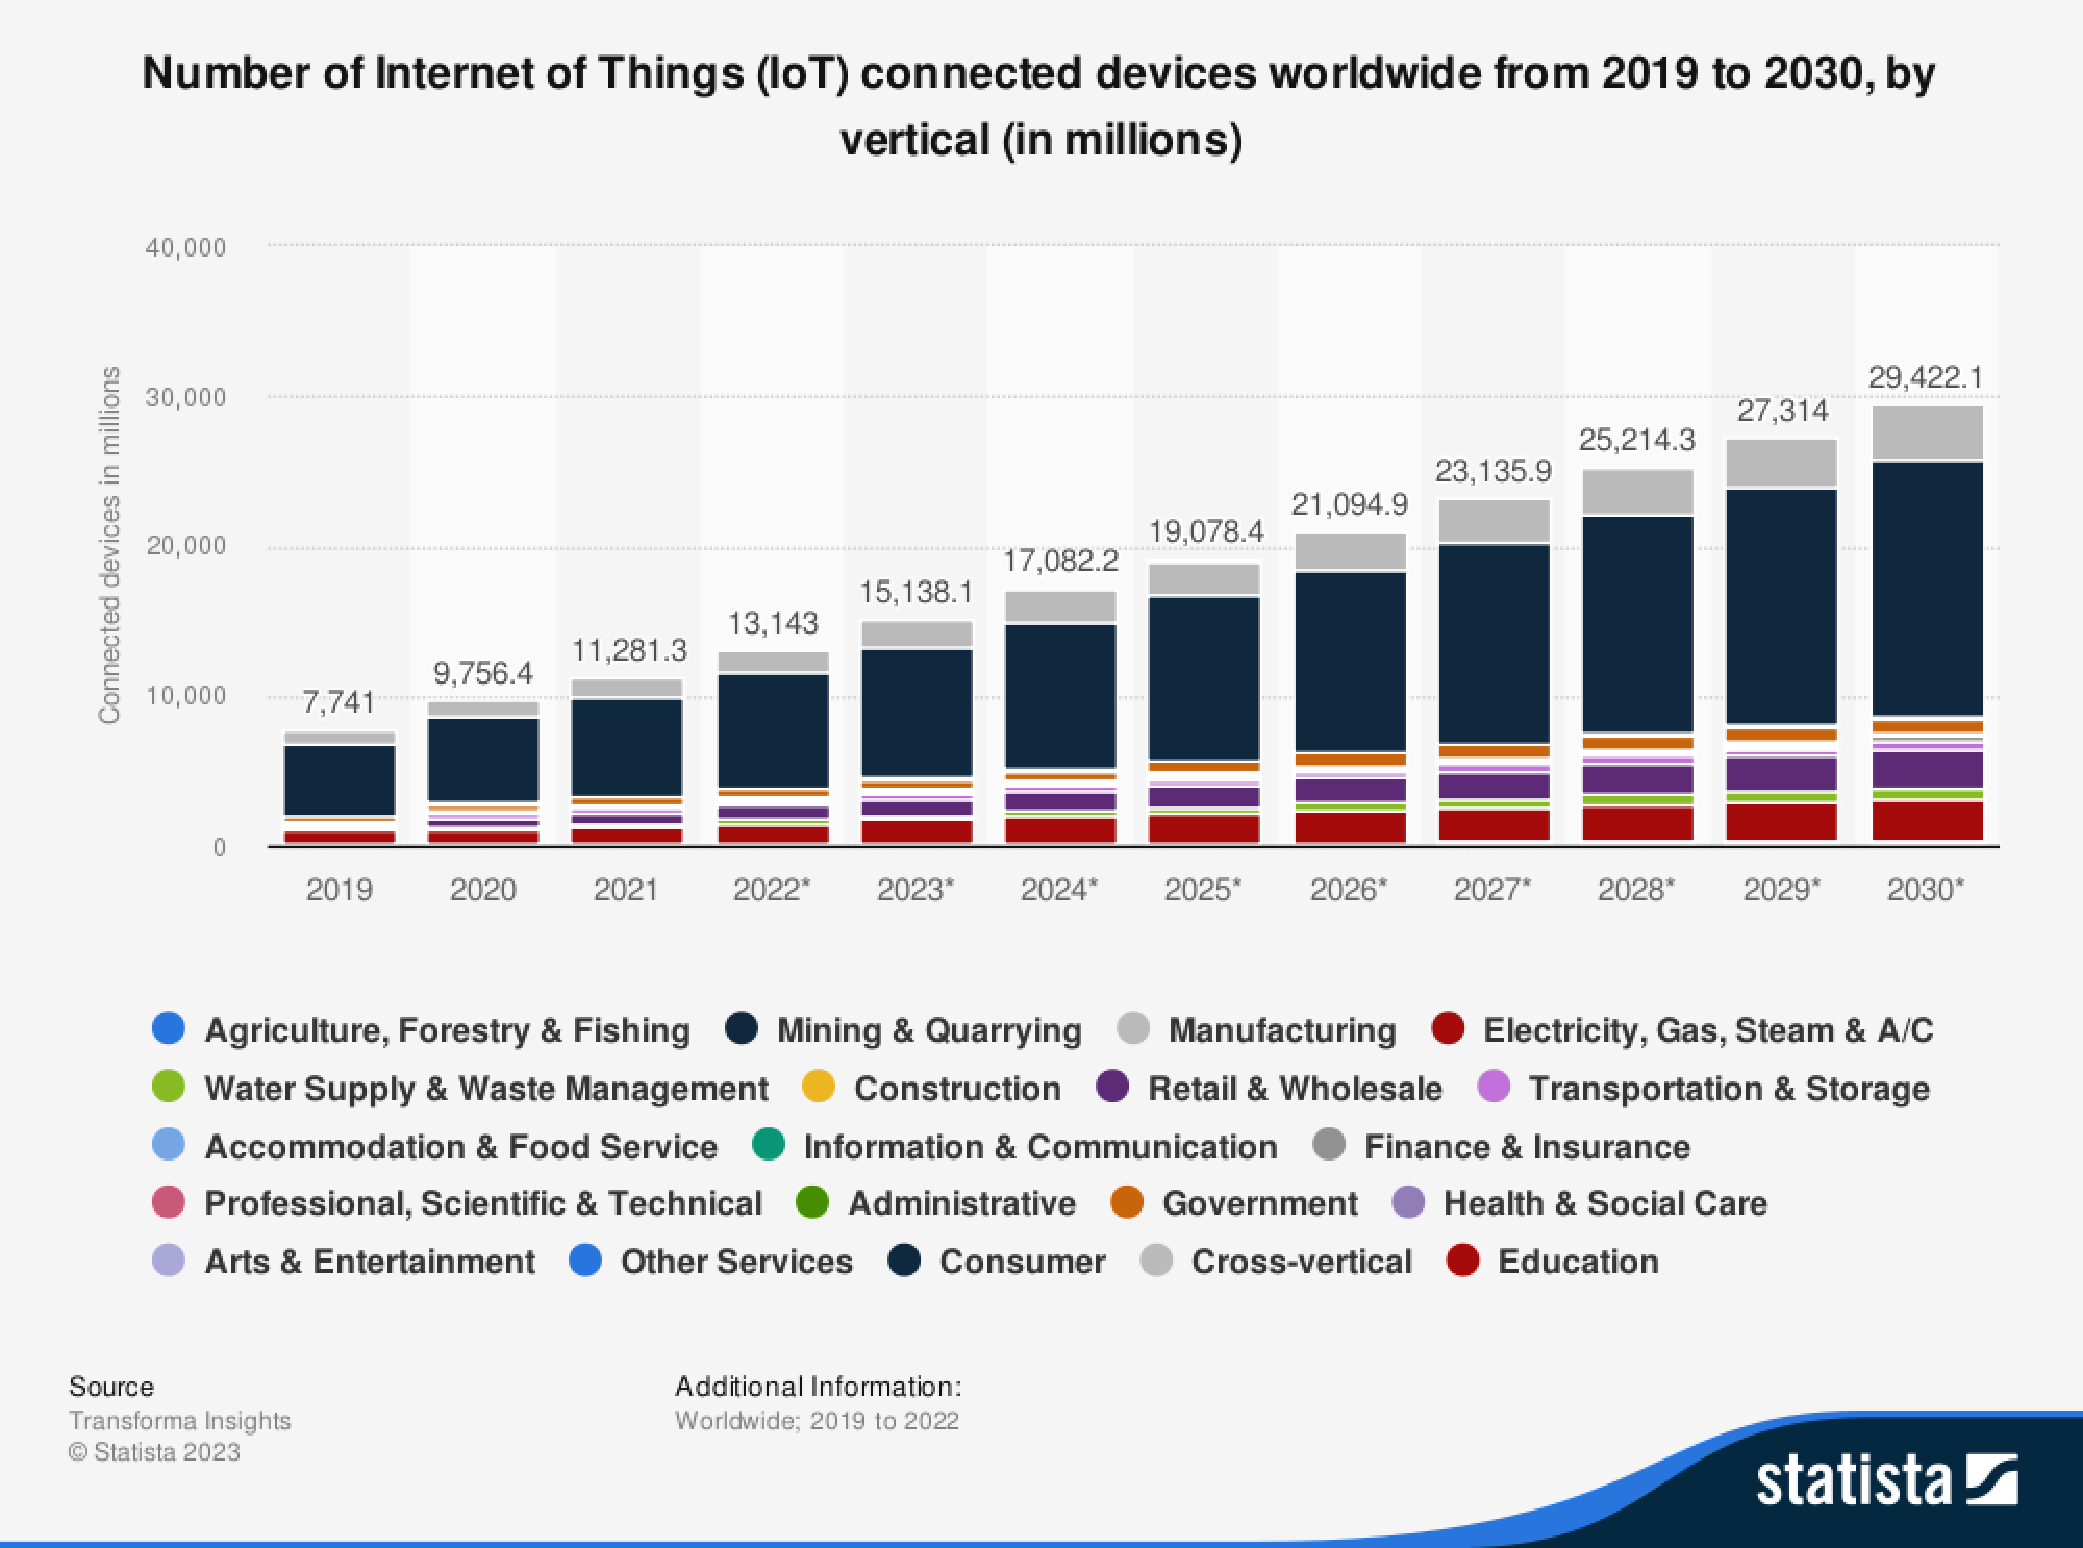
\includegraphics[scale=0.4]{Images/devices_forecast.pdf}
\caption[Number of Internet of Things (IoT) connected devices worldwide from 2019 to 2030, by vertical]{Number of Internet of Things (IoT) connected devices worldwide from 2019 to 2030, by vertical. The single largest use case in terms of the number of Internet of Things (IoT) connected devices is consumer internet and media devices, accounting for a third of all devices worldwide in 2030. The other two largest use cases are smart grid (e.g. smart meters) and connected vehicles - Statista \cite{StatistaIoT2023}}
\label{F_devices_forecast}
\end{figure} 
\textbf{Security and privacy risks.}
The Internet of Things (IoT) is bringing new ways to collect data, analyze them and take decisions
for developing applications that answer or even anticipate the users’ needs. The unprecedented nature of the IoT has consequences on the data generated, which are \emph{fine-grained} and in \emph{quantity}.\sul{ The collected data enables the monitoring of users' actions and locations while users are often unaware of the data collection}. For these reasons, the data are particularly
privacy-sensitive, requiring efficient privacy-preserving mechanisms. Moreover, the IoT has unique
characteristics due to the extreme heterogeneity and large quantity of objects it can interconnect, as
well as the spontaneous nature of their interactions, making it a distributed system of unprecedented
scale. It results in several security complications, as some IoT devices, e.g., sensors, may not have the computation power or storage needed to implement 
cryptographic primitives. Additionally, IoT devices may have security vulnerabilities in their firmware, software, or hardware components. These vulnerabilities can be exploited to gain control over devices, disrupt their functionality, or launch attacks on other devices or networks \cite{Omolara2022}.

\textbf{Regulation.} Furthermore, the EU General Data Protection Regulation (GDPR) \cite{EUdataregulations2018} introduces several legal obligations, among which \emph{privacy-by-default}, \emph{consent management} and \emph{accountability}. Indeed, companies - outside of the legitimate interest - have to explicitly ask the user,
as a data owner, for clear, positive and explicit consent before any data collection. Whatever the
interests at stake, a company has to prove at any time that data processing is always performed
legitimately, either according to the user’s consent or for a legitimate purpose.

\textbf{Requirements for a secure Internet of Things.}
\cul{As a consequence of the security and privacy risks peculiar to the Internet of Things, the requirements for a secure and privacy-preserving Internet of Things are the following. First, the solution must consider} \emph{constrained devices},
\cul{and ensure the security and privacy threat mitigations are not disconnected 
from IoT's actual capacities. For example, cryptography-based solutions are often inapplicable to Internet of Things devices. Second, as data are privacy-sensitive, it is compulsory for user's privacy to enforce} \emph{access control} on their data and to \emph{monitor the usage of their data}. \cul{Third, for performance, security and privacy purposes, decentralization is an important aspect in the Internet of Things. Centralized entities such as cloud servers may snoop on users' data}~\cite{Qin2020} and can be vulnerable to accidental disclosures or external attacks~\cite{Qin2020}. Availability can be a matter of concern too, as physical infrastructure can be damaged, e.g. because of a fire or a natural disaster~\cite{Ayoub2021}. Furthermore, centralization hinders performance, specifically by increasing the deployment and maintenance cost~\cite{Salimitari2020}, which in turn hinders scalability.

\textbf{Leveraging distributed ledgers for the Internet of Things.} \cul{Distributed ledger technologies (DLTs), due to inherent properties, are a promising solution to address the Internet of Things requirements for security. DLTs indeed provide a certain degree of \emph{decentralization} and are \emph{tamper-proof} which is useful for a wide range of security applications ranging from trust management} \cite{Liu2023} \cul{to anonymous and secure transactions} \cite{Bothra2023}. \cul{DLTs can also be used to provide access control in an automated and transparent fashion using \emph{smart contracts}} \cite{Bao2023}. \cul{However, distributed ledger technologies are not always designed for the Internet of Things requirements. Performance, security and privacy requirements call for well-tailored distributed ledgers, that provide anonymous, efficient and cheap transactions for IoT-constrained devices.}

\section{Problem statement}
\label{S_problem_statement}
\sul{In this part, several challenges related to the Internet of Things are highlighted
and are used to identify \emph{research objectives}. These objectives will provide the connecting thread throughout this document.}
\paragraph{Micro-transactions.} In the Internet of Things, data collection often serves business purposes and requires financial transactions afterward to buy and sell the data. Data trading is based on \emph{micro-transactions}, which should be processed with the minimum possible fee as regards the data value. Additionally, several Internet of Things real-life scenarios without data trading require micro-transactions. Such use cases include \emph{parking meters} in smart cities, where the drivers would be charged automatically for the amount of time they park their vehicles. In \emph{Industrial Internet of Things} (IIoT), IoT devices could monitor machinery and equipment and automatically order replacement parts for improved maintenance. The manufacturer could be charged a small fee for the replacement parts, with the payment occurring automatically via micro-transactions.

Overall, micro-transactions can provide new revenue streams for businesses by enabling them to monetize data generated by IoT devices and 
increase the efficiency of business operations by enabling automated payments.
However, it is important to ensure that privacy and security are maintained to protect sensitive data due to the Internet of Things context and financial transactions involved.
The latter issues as well as the need for efficient, micro-transactions in the IoT leads to the first research objective of this thesis:
\begin{mdframed}[ skipabove=20pt, skipbelow=20pt, innertopmargin=12pt, innerbottommargin=12pt] 
\phantomsection    
\begin{center}
     \emph{Objective 1: Achieve privacy-preserving zero-fee transactions for the Internet of Things} 
     \label{obj:1}
\end{center}
\end{mdframed}

%\paragraph{Distributed ledgers and privacy-enhancing technologies.} To make transactions, blockchains or distributed ledgers in general are technologies of interest in IoT settings due to their inherent distribution.
%Besides, due to its unique properties, the use of distributed ledger technologies with privacy-enhancing technologies, including usage control, has been widely discussed in the literature \cite{Cha2019}. There are three main categories for the use of distributed ledgers in PETs: access control, auditing and data storage \cite{Cha2019}.  
%Notably, distributed ledgers are used for their smart contracts to define and enforce access policies of the data \cite{Khan2020, Zhaofeng2021, Bao2023, Rifi2017}. As regards usage control, several works have been conducted in private blockchain settings \cite{Khan2020, Zhaofeng2021, Shi2021}. While private blockchains benefit from low latency, they lack some beneficial features of public distributed ledgers such as total distribution with highly secure and immutable data storage. Besides, the network overhead increases rapidly with the number of nodes in the PBFT consensus protocol, commonly used by private blockchains.  \cite{Salimitari2020}. Distributed ledgers often have performance constraints that do not meet IoT requirements, such as the number of transactions per second \cite{Salimitari2020}.

\paragraph{Distributed ledgers and usage control.} To process transactions, blockchains or distributed ledgers in general are technologies of interest in IoT settings due to their inherent distribution.
Besides, due to its unique properties, the use of blockchains jointly with usage control has been widely discussed in the literature. \sul{Usage control can be considered as an extension of access control, which continuously monitors data once access has been granted. It grants or denies access based on \emph{authorizations}, \emph{obligations}, which have to be fulfilled to be granted access, and finally on \emph{conditions}
related to the system state. As a consequence, usage control is beneficial to users' privacy as they can decide who may access their data and how the data are used.}

Several works combining usage control and blockchains have been conducted in private blockchain settings \cite{Khan2020, Shi2021, Zhaofeng2021, Zhang2022}. While private blockchains benefit from low latency, they lack some beneficial features of public distributed ledgers such as total distribution with highly secure and immutable data storage. Besides, the network overhead increases rapidly with the number of nodes in the PBFT consensus protocol, commonly used by private blockchains.  \cite{Salimitari2020}. Distributed ledgers often have performance constraints that do not meet IoT requirements, such as the number of transactions per second \cite{Salimitari2020} \sul{which is around 6 transactions per second (TPS) for the Bitcoin blockchain excluding use cases with numerous simultaneous transactions. The size of the transaction ledger can be a hurdle to IoT adoption as well. The Bitcoin blockchain has grown to 475 GB as of June 8, 2023, which is impossible to store on lightweight devices} \cite{StatistaBTC2023}

 Even though the literature proposed integration schemes for usage control in distributed ledgers \cite{Khan2020, Shi2021}, the general principles of integration are not properly identified. In particular, solving the potential bottleneck issues, as well as the identification of criteria for integration, are not well addressed by the current research.
Considering these current limitations, this thesis identifies the following research objectives: 
\phantomsection 
\begin{mdframed}[ skipabove=20pt, skipbelow=20pt, innertopmargin=12pt, innerbottommargin=12pt] 
\begin{center}
     \emph{Objective 2: Identify the distributed ledgers appropriate for the Internet of Things} 
    \newline


   \emph{Objective 3: Design a method to integrate usage control in distributed ledger technologies efficiently}
   \label{obj:23}
\end{center}
\end{mdframed}
\paragraph{Data usage control modeling in distributed systems.}
A formal model of data usage control can help ensure that the system's security and privacy goals are achieved by providing a clear specification of the access control policies, the resources to be protected, and the roles and responsibilities of the participants in the system. 
While this modeling has been repeatedly discussed in the state of the art in centralized settings \cite{Pretschner2011, Kelbert2013, Kelbert2014, Fromm2020}, it is still incomplete in distributed systems \cite{Gil2023}, considering only the distribution of the usage control system (UCS) components, but not of the other system users, such as the policy makers and the data readers \cite{Kelbert2015, Kelbert2018}.
In the Internet of Things, due to performance, security and privacy concerns, distributed systems are widely used, requiring 
an appropriate model to describe information flows and data policies. This leads to the introduction of the fourth research objective:
\phantomsection 
\begin{mdframed}[ skipabove=20pt, skipbelow=20pt, innertopmargin=12pt, innerbottommargin=12pt] 
\begin{center}
     \emph{Objective 4: \cul{Identify concepts relevant to the Internet of Things and missing from the current usage control formalism in distributed systems}} 
     \label{obj:4}
\end{center}
\end{mdframed}

\textbf{Validation of the proposed solutions.} \cul{As part of the previous research objectives (Objectives 1 to 4), several solutions will be proposed in this thesis work to address specific issues in the Internet of Things. As regards the performance, security and privacy constraints of the IoT, it is necessary that: 1) the security and the privacy of these solutions are assessed; 2) the solutions are tested using \emph{proof of concepts} to ensure their feasibility, in particular, as regards performance.} \cul{These requirements lead to 
the last set of research objectives}:

\phantomsection 
\begin{mdframed}[ skipabove=20pt, skipbelow=20pt, innertopmargin=12pt, innerbottommargin=12pt] 
\label{obj:5_6}    
    \begin{center}
         \emph{Objective 5: Analyze the security and privacy of the proposed methods with security and/or privacy threat assessment} 
        \newline
    
    
       \emph{Objective 6: Validate the feasibility of the proposed methods with 
       a proof of concept}
       \newline 
       
       %\emph{Objective 7: Validate the modeling of data usage control in distributed systems using model checking}
       \label{obj:56}
    \end{center}
    \end{mdframed}

\section{Assumptions}
\label{S_assumptions}

The Internet of Things encompasses a wide range of use cases with different requirements and specific research questions. As a consequence, this section explains the context considered in this thesis. Several definitions are first provided to clarify some notions such as the Internet of Things. \rul{The initial assumptions at the start of the Ph.D. are then provided, to highlight the results of the analysis of the state of the art.} The precise context considered is finally given to define the scope of the conducted research.

\paragraph{Definitions.} The \emph{Internet of Things}, i.e., IoT for short, has been first used in 1999 by MIT's Kevin Ashton when he promoted the RFID technology \cite{Zhang2020}. The Internet of Things has since disrupted the classic Internet by introducing devices embedded in everyday objects, sending and receiving data by themselves. However, the actual definition of the Internet of Things is loose and is often referred to using other words such as \emph{smart home} outside academia and industry \cite{Berte2018}. The National Institute of Standards and Technology (NIST) agrees with the lack of a universal definition of the Internet of Things but proposes the two following \emph{fundamental concepts} of the IoT \cite{NISTIR8200}:
\begin{center}
\begin{mdframed}[ skipabove=20pt, skipbelow=20pt, innertopmargin=12pt, innerbottommargin=12pt] 
\begin{itemize}
    
    \item[(1)] \emph{IoT components are connected by a network providing the potential for a many-to-many
relationship between components (the network capability may or may not be
Transmission Control Protocol/Internet Protocol (TCP/IP) based)};
    \item[(2)] \emph{Some IoT components have sensors and actuators that allow the components to observe
(collect data about) and affect the physical world.}
\end{itemize}
\end{mdframed} 
\end{center}

These two concepts are of interest as they reflect the \emph{high number of devices}, the \emph{heterogeneity} both in terms of protocols and devices, and the link between the IoT devices and the physical world.

Similarly, \emph{privacy} is repeatedly mentioned in this thesis but is not an easy concept to define. It is recurrently discussed in the literature \cite{Moore2008,  Alibeigi2019, Tang2021, Elmimouni2023} and derived to more precise concepts, such as \emph{usable privacy} \cite{Malkin2023} which refers to the implementation of user-friendly privacy-preserving mechanisms. For privacy, the two following definitions are proposed, first to emphasize the interdisciplinary aspect of privacy, then a definition more related to data and computer science, also called \emph{information privacy}:

\begin{center}
\begin{mdframed}[ skipabove=20pt, skipbelow=20pt, innertopmargin=12pt, innerbottommargin=12pt] 
\begin{itemize}
    \item[(1)] \emph{Broadly speaking, privacy is "the right to be let alone" \cite{Warren1890}, or freedom from interference or intrusion}; 
    \item[(2)] \sul{\emph{Privacy is the claim of individuals, groups, or institutions to determine for themselves when, how, and to
    what extent information about them is communicated to others}} \cite{Westin1968}.
\end{itemize} 
\end{mdframed}
\end{center}

\cul{To further clarify the notion of privacy, we list the privacy properties of interest for this thesis work. 
Users tend to provide excessive information to
service providers and to lose control of their personal information. Therefore, the \emph{content awareness (1)} property is proposed} \cite{Wuyts2015}
 \cul{to make sure that users are aware of their personal data
and that only the minimum necessary information should be
shared and used for data processing.
The more personally identifiable information a data subject discloses, the higher the risk is for a privacy violation. To
ensure content awareness, several technical enforcement tools have been developed such as the personal information feedback tools} \cite{Patil2009} \cul{to help users gain privacy awareness and self-determine which personal data to disclose.}

\cul{Unlike the user-centric content awareness property, the \emph{policy and consent compliance} property (2)} \cite{Wuyts2015} \cul{requires
the whole system, e.g., including data flows, data stores, and
processes, as a data controller to inform the data subjects
about the system's privacy policy, or allow the data subjects
to specify consent in compliance with the legislation. These two properties are often referred to as 
\emph{soft privacy}} \cite{Wuyts2015}. \cul{\emph{Hard privacy} focuses on 
providing as little data as possible to reduce the need to trust other entities, which is referred to as \emph{data minimization}. On the contrary, soft privacy is based on the assumption
that data subjects have already no control over their personal data and must
have confidence in data controllers. The
data protection purpose of soft privacy is therefore to provide data security and process data with specific purpose and consent,
using policies, access control, and audit}.  

\paragraph{\rul{Initial assumptions.}} \rul{To provide a better understanding of the contributions of this thesis work, we describe here the assumptions at the beginning of the Ph.D. work. First, the initial research questions were the following:}

\begin{enumerate}
    \item Which privacy-enhancing technologies are suitable for the Internet of Things? 
    \item How to enable usage control in distributed IoT platforms in an efficient way?
\end{enumerate}

\rul{While doing the state of the art, which is summarized in the dedicated Chapter} \ref{C_state_of_the_art}, \rul{it appeared that instead of identifying PETs for the Internet of Things, it was more relevant to address performance and security requirements, then to implement privacy-enhancing technologies on the chosen technologies. Indeed, privacy-enhancing technologies can add overhead to the already performance-demanding Internet of Things. Addressing privacy before the performance aspects would be poorly satisfying, due to the impossibility to implement the proposed privacy-preserving solutions in practice. As a result of the analysis of the state of the art, blockchains, first of all, then distributed ledgers appeared as a technology of interest for performance and security. Indeed, blockchains are decentralized by nature and address numerous issues existing in centralized networks, including availability with the removal of a single point of failure, but also performance with better scalability, reduced maintenance costs and reduced update costs} \cite{Salimitari2020}.

% \rul{No hypothesis on the most suitable blockchain technology was formulated at the beginning of the Ph.D., nor were the scenarios used in Chapter} \ref{C_solving_trilemma} \rul{and Chapter} \ref{C_formalism} \rul{defined}.

\paragraph{Context.} In this thesis, only \emph{large-scale IoT deployments} are considered, as use cases involving a moderate amount of devices are already well addressed by the state of the art. Large-scale IoT deployments have specific issues regarding scalability, heterogeneity and performance constraints on devices that require dedicated, well-tailored solutions. For instance, private blockchains, often considered as an IoT-friendly technology \cite{Asheralieva2021}, are actually not well-suited for large-scale deployments of devices. 

Second, the scenarios considered will require \emph{payments}, as IoT devices can be used in real-life to generate and sell data or buy actual goods, e.g., vending machines. Finally, the Internet of Things features a high diversity of devices. This \emph{heterogeneity} of devices is considered in this thesis, which implies that constrained devices, e.g., in terms of computing power, memory, energy storage..., are involved in the network. This last assumption markedly restricts the use of several security and privacy tools, such as encryption. \rul{While this thesis work considers the heterogeneity of devices, it does not address every Internet of Things use-cases. For instance, the Industrial Internet of Things devices may operate in a closed environment preventing them from selling the data to outside agents. Besides, actuators do not have an obvious incentive to trade their data or even generate data in the first place.}

\rul{For a better understanding, we provide scenarios where data trading could be relevant:}
\begin{itemize}
    \item \emph{agriculture and precision farming}: farmers can collect data from IoT sensors installed in fields to monitor soil moisture, temperature, humidity, and crop growth. This data could be aggregated and sold to agricultural technology companies or research institutions to improve crop yield and develop new farming techniques;
    \item \emph{smart city infrastructure}: municipalities can gather data from IoT devices deployed throughout the city to monitor traffic patterns, air quality, waste management, and energy consumption. This data could be valuable for urban planning, transportation optimization, and environmental monitoring, and could be sold to city planners or companies working on smart city solutions;
    \item \emph{smart home}: manufacturers of smart home devices, such as thermostats, security cameras, and smart appliances, might offer users the option to sell usage data. This data can provide insights into user preferences and usage patterns, helping manufacturers refine their products;
\end{itemize}
\rul{Conversely, the following families of scenarios are out of the scope of this thesis:}
\begin{itemize}
    \item \emph{closed environments}, such as \emph{manufacturing} where there is a lack of incentive to buy or sell actuator data; 
    \item \emph{specific legislations}, such as medical data legislations in the \emph{e-health} sector. Several legislations have strict rules as regards the selling of medical data, for privacy reasons. Data trading may be impossible in some use cases, or without the clear and explicit consent of the users.
\end{itemize} 

\section{Contributions}

This thesis addresses the defined research objectives with the following contributions:

\begin{itemize}
    \item the design of a framework to address the requirements of privacy, security and performance of the Internet of
Things (Chapter \ref{C_solving_trilemma}). The basis of the framework is the IOTA technology, a distributed ledger relying on a directed acyclic graph to create zero-fee transactions, instead of a blockchain (\hyperref[obj:1]{\emph{Objective 1}} and \hyperref[obj:23]{\emph{Objective 2}}). A security and privacy threat assessment is conducted on the proposed solution using an illustrative scenario of a car sharing system (\hyperref[obj:56]{\emph{Objective 5}} and \hyperref[obj:56]{\emph{Objective 6}});
\item an integration method of usage control with distributed ledgers (Chapter \ref{C_integration}). Suitable DLTs are determined according to specified parameters, and a proof of concept is proposed for performance evaluation (\hyperref[obj:23]{\emph{Objective 3}} and \hyperref[obj:56]{\emph{Objective 6}}). A privacy threat assessment using LINDDUN is also conducted (\hyperref[obj:56]{\emph{Objective 5}});
\item an extension of a decentralized model for usage and
information flow control in distributed systems, introducing a policy jointly defined over collective personal data and \cul{ considering the
availability of the different individual parts of the distributed system} (\hyperref[obj:4]{\emph{Objective 4}});
\end{itemize}

\textbf{Framework for performance, privacy and security in the Internet of Things. } 
This first contribution (\emph{Contribution 1}) proposes a newly designed framework to address the requirements of privacy, security and
performance of the Internet of Things. In this contribution, we first identify IOTA as the basis of the framework and demonstrate its relevance. IOTA indeed unlocks distributed ledger performance by increasing throughput as more users join the
network thus making the network scalable. Additionally, IOTA does not rely on miners to add transactions to the ledger, enabling zero-fee transactions. Not designed for privacy protection, IOTA is complemented in the framework by privacy-preserving mechanisms: merge avoidance
and decentralized mixing. Finally, usage control mechanisms are introduced so that users can monitor the use and dissemination of their data.

\textbf{Integration of usage control with distributed ledgers.} This contribution  (\emph{Contribution 2}) proposes to integrate usage control with distributed ledgers based on directed
acyclic graphs (DAG). The benefits of integration are: 1) the components of the usage control system contribute
to the network security, as a node; 2) the usage control
system processes the transaction data without intermediaries,
which is faster and more reliable. An analysis of
distributed ledgers is provided based on their features, to determine which
ledgers are suitable for the proposed integration. An implementation of usage control integration is proposed on IOTA. Performance tests are conducted on this implementation, showing approximately a 90\% decrease
in the time needed to push transactions and make an access decision when the UCS is integrated.

\textbf{Data usage control modeling in distributed systems.} The last contribution (\emph{Contribution 3}) of this thesis work is the proposition of an extended usage control model \sul{going beyond the state of the art} that integrates decentralized information flow control (DIFC). DIFC enables users to decide collectively which policy to apply to their common data, \sul{further distributing the network by decentralizing the policy definition to the users}.
Architectural aspects and formal definitions to enable decentralized policies for shared data are proposed as a novelty, resulting from the DIFC integration.
Unreliable and intermittent distributed systems are also considered, as a distinctive characteristic in some Internet of Things use cases, e.g., low-energy devices. 

\section{Acknowledgments}

This thesis work and the associated Ph.D. have been funded by the
Futures \& Ruptures program of Foundation Mines-Télécom. It is also partially supported by the Institut Mines-Télécom VP-IP Chair on Values and Policies of Personal Information (\url{https://cvpip.wp.imt.fr}) and by the 3rd Programme d’Investissements d’Avenir [ANR-18-EUR-0006-02]
within the framework of Energy4Climate Interdisciplinary Center (E4C) of IP Paris and Ecole des Ponts ParisTech (\url{https://www.e4c.ip-paris.fr/}). 

\section{Thesis outline}

This document is structured as follows. Chapter \ref{C_state_of_the_art} provides the necessary background on usage control and distributed ledgers, then the state of the art and \cul{its current limitations in addressing the different objectives of the problem statement} (cf. Section \ref{S_problem_statement}). Chapter \ref{C_solving_trilemma} details the design of a framework (\emph{Contribution 1}) to simultaneously address performance, security and privacy requirements in the Internet of Things and enable micro-transactions (\hyperref[obj:1]{\emph{Objective 1}}). \sul{The framework is based on the IOTA distributed ledger, and its security and privacy are evaluated on a car-sharing use case}. Chapter \ref{C_integration} details the integration of usage control with distributed ledgers (\emph{Contribution 2}) to further improve the performances of both the distributed ledger and usage control system. Chapter \ref{C_formalism} addresses the issues in defining a formalism for usage control in distributed systems and justifies the use of decentralized information flow control to complete the state-of-the-art formalism (\emph{Contribution 3}). The final Chapter \ref{C_conclusion} concludes this thesis with a summary of the thesis, the future works and the limitations considering both the research objectives and the scope of this research work.
A glossary (Appendix \ref{A_glossary}) provides definitions and explanations for some notions 
for better understanding.
The complementary appendices (Appendix \ref{A_cryptocurrencies}, Appendix \ref{A_usage_control}) provide additional general information on the different technologies 
addressed in this thesis.  

%-------------------------------------------------------------------------------
\newpage \ \newpage
\chapter{\rul{State of the Art on Usage Control and Distributed Ledgers}}

\label{C_state_of_the_art}
\minitoc
In the previous chapter, usage control and distributed ledgers are identified as key technologies for Internet of Things privacy, provided that the distributed ledger can handle requirements in terms of performance. In this chapter, we will introduce the state of the art on \emph{usage control} (Section \ref{S_usage_control}), a privacy-enhancing technology enabling fine-grained dynamic control over the data.

Modern usage control systems now integrate \emph{Information Flow Control} (IFC), a technology that enables the monitoring of the information flow in a system to prevent undue dissemination. The control of information flow, which is compulsory for efficient usage control as it prevents data from escaping the monitoring scope of the usage control system, will be introduced in Section \ref{ss_information_flow_control}. 

Afterward, the state of the art on distributed ledgers will be provided (Section \ref{S_distributed_ledgers}), before focusing on specific IoT aspects. 
Then, distributed ledger privacy (Section \ref{S_privacy_DLT}) and performance (Section \ref{S_DLT_performance}) will be introduced, 
as these two topics are closely related to the Internet of Things concerns.

\rul{A critical analysis of the various technologies and solutions presented is also provided in this chapter, in order to highlight relevant criteria to assess the compatibility with the Internet of Things (Sections} \ref{ss_blockchain_DLT} \rul{and} \ref{ss_performance_consensus_methods} \rul{in particular})
\section{Usage control}
\label{S_usage_control}

In the first chapter, we mentioned usage control as a potential privacy-enhancing technology for the Internet of Things, which could be used jointly with distributed ledgers with the proper integration scheme (\hyperref[obj:23]{\emph{Objective 3}}). In this section, the needed notions of usage control are introduced for a better understanding of this document (Section \ref{ss_ucon_elementaries}), before introducing the system architecture of usage control systems (Section \ref{ss_ucon_architecture}). 
\subsection{Usage control elementaries}
\label{ss_ucon_elementaries}

\paragraph{ABC model.} Usage control is an extension of access control, describing how the data can be used after initial access. It was first proposed by Sandhu and Park as the \emph{UCON} model~\cite{Park2004}. This model extends traditional access control by introducing attribute mutability, as well as new decision factors described by the ABC model (Figure \ref{F_ABC_model}): \emph{Authorizations, oBligations, Conditions}.
In addition, the ABC model considers \emph{subjects and objects}, classic components of traditional access control, and their attributes i.e., \emph{subject attributes} and \emph{objects attributes}. 
\emph{Subject} and \emph{object} are notions taken from access control, such that a \emph{right} enables a subject to access an object in a particular mode e.g., read, write. Note that in usage control, the right does not exist as such, but is determined when the access is initiated by the subject and considering other ABC components. \emph{Usage decision functions} are designed 
to make the determination of a right's existence based on subject and object attributes, authorizations, obligations and conditions.
\emph{Subject} and \emph{object attributes} are properties that can be used during the access decision process. Subject identity is an example of useful subject attributes, but is not mandatory
as it would exclude the possibility of anonymous services. Examples of object attributes are security labels and access-control lists. 

One of the most important innovations of UCON is the introduction of \emph{mutable attributes} that are modified as a consequence of access, while \emph{immutable attributes} are changed as a 
result of administrative action. This is a critical differentiator compared to most access control models and is particularly relevant in IoT contexts due to the dynamicity of the network.
\begin{figure}[t]
\centering
 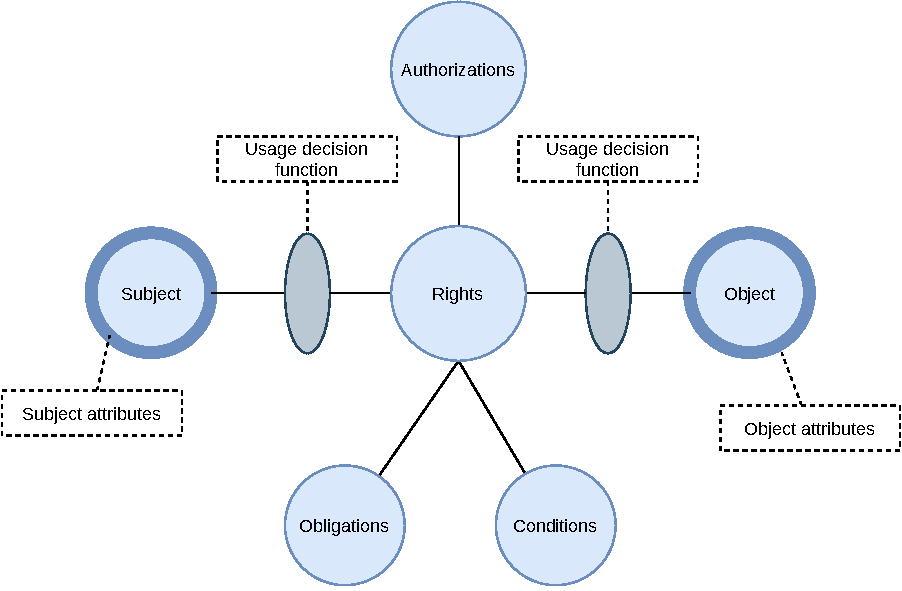
\includegraphics[width=0.8\textwidth]{Images/abc_model.pdf}
\caption{ABC model as defined by Sandhu and Park \cite{Park2004}}
\label{F_ABC_model}
\end{figure} 

 \emph{Obligations} are requirements to be fulfilled by the subject to be granted access. \emph{Conditions} are subject-independent environmental requirements for allowing access. Since attributes are mutable, \cul{authorizations can be checked and obligations fulfilled before or during the access}. They are referred to as pre-authorizations and ongoing-authorizations, or respectively pre-obligations and on-going obligations.
Improving user control over the data is crucial to achieving privacy in IoT systems~\cite{Cha2019}, and usage control provides the technical basis to do so.

\paragraph{Related technologies.} Modern usage control systems rely on information flow control, particularly to prevent data dissemination to uncontrolled areas. Information flow control is extensively discussed in Section \ref{ss_information_flow_control}. Besides, to monitor the use of the data, the usage control system needs to access system calls. This process is intrusive and is a threat to data readers' privacy which must be protected as much as the monitored data. 
To achieve privacy-preserving enforcement of the usage control rules, usage control usually relies on a \emph{Trusted Execution Environment} (TEE)~\cite{Shi2021}. A trusted execution environment is an area on the main processor of a device that is separated from the system's main operating system. It ensures that data is stored, processed and protected in a secure environment. In particular, the data loaded inside a TEE is guaranteed to be protected as regards \emph{integrity} and \emph{confidentiality}. The TEE is installed on the monitored user's machine, to prevent undue processing or dissemination of the monitored data.


\subsection{Usage control architecture}
\label{ss_ucon_architecture}

The components of the usage control system are depicted in Figure \ref{F_ucon_components}. Note that different implementations of a usage control system may not implement every component, or conversely design additional ones. For instance, Martinelli \emph{et al.} \cite{Martinelli2019} introduces components dedicated to the evaluation of obligations called \emph{Policy Obligation Point} to manage distinct kinds of obligations.
\begin{figure}[t]
\centering
 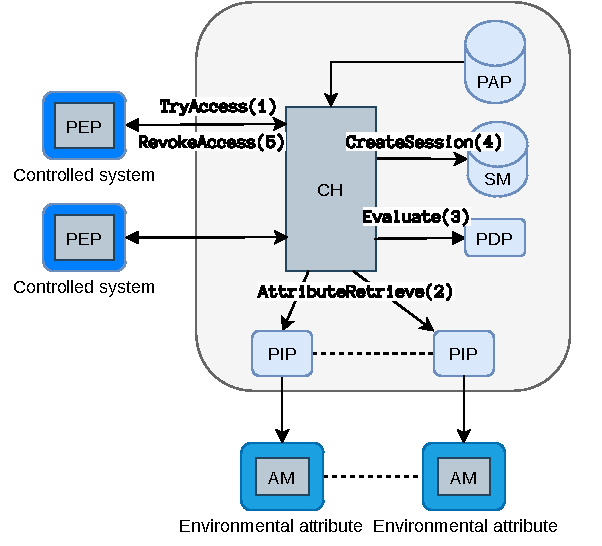
\includegraphics[scale=0.9]{Images/ucon_framework.pdf}
\caption{Usage control architecture, based on~\cite{Rizos2019}}
\label{F_ucon_components}
\end{figure}

The \emph{Usage Control System} (UCS) interacts with \emph{Environmental Attributes} through \emph{Attribute Managers} (AM) to recover the values of the attributes, and with the \emph{Controlled Systems}. 
\begin{itemize}
    \item \emph{PDP}: the Policy Decision Point in charge of the policy evaluation. It takes as input an access request, 
    the corresponding policy and the attributes of both users and context. Then it returns the result of the evaluation: \emph{Permit, Deny, Undetermined};
    \item \emph{PAP}: the Policy Administration Point, which is responsible for creating, modifying, and deleting policies based on the needs of the system and the requirements of the users. It is also the storage point of the policies in the usage control system;
    \item \emph{PEP}: the Policy Enforcement Points are embedded in the Controlled Systems, and intercept access requests and trigger the UCS decision-making process. The PEPs then enforce the policy evaluation result on the Controlled System which requires an access;
    \item \emph{PIP}: the Policy Information Point, an interface so that the UCS can retrieve the values of the attributes from the system environment;
    \item \emph{CH}: the Context Handler, in charge of routing the different processes;
    \item \emph{SM}: the Session Manager stores all active sessions and the information needed for monitoring their status. The SM is composed of an \emph{Access Table} that stores information about the current ongoing sessions to be able to continuously enforce policies. Usually, Access Tables are implemented by a database whose entries refer to a session and contain at least the session identifier, the access request and the session status i.e., pending, active, revoked or ended.
\end{itemize}


\textbf{Workflow.} The workflow between the different components of the usage control system after receiving an access request is shown in Figure \ref{F_ucon_components} and is composed of the following messages \cite{Rizos2019}. When a user requires access, the PEP sends a \texttt{TryAccess} message to the CH. The CH fetches the environmental attributes from the PIP (\texttt{\justify AttributeRetrieve}) and the policy from the PAP, and forwards them to the PDP to evaluate the policy (\texttt{Evaluation}). The PDP decides to accept or reject the request with a
 \emph{PERMIT} or a \emph{DENY} message, then sends the decision to the CH which forwards it to the PEP. If the answer is \emph{PERMIT}, a unique SessionId is assigned to the access request (\texttt{createSession}) and the Session Manager (SM) is updated. The PEP then sends a \texttt{startAccess} message to the CH, to signal the start of the access. If the UCS detects a policy violation during the continuous monitoring, the CH informs both the PEP and the SM that the session is terminated by sending the \texttt{revokeAccess} message. It is also possible that the user asks to end the session itself, by sending the \texttt{endAccess} message. The CH tells the SM to delete the session details, and the PIP to unsubscribe the attributes related to this session.

\subsection{Information flow control}
\label{ss_information_flow_control}

We introduced usage control as a dynamic and flexible access control technology. It enables data owners to enforce policies for their data, 
by defining authorizations, but also obligations, which are actions to be performed before, during or after being granted access, and conditions bearing on the system and environment attributes, e.g., the time.

 Several methods exist to limit information disclosure, including usage control but also access control lists, firewalls or cryptography. However, although these methods do impose limits on the information that is released by a system, they do not provide any guarantees about information \emph{propagation}. 
 Monitoring data dissemination is valuable in information security to prevent leaks, but also for usage control as information could be disseminated outside the scope of the usage control system. 
 \emph{Information Flow Control} (IFC) is a mechanism introduced to enforce information flow policies in a system. Several methods to implement information flow control have been proposed in the literature:
 \begin{itemize}
    \item Run-time mechanisms that tag data with \emph{information flow labels} have been employed at the operating system level and the programming language level \cite{Hu2021};
    \item \emph{Static program analyses} have also been developed to ensure information flows within programs conform with policies \cite{Zheng2007};
 \end{itemize} 

 \textbf{Taxonomy.} Information flow control techniques can be characterized and compared using the following features \cite{Denning1976, Hu2021}. 
\begin{enumerate}
    \item \emph{Operator precision}: How are security classes updated? 
    \begin{itemize}
        \item Conservative: IFC uses a least upper bound;
        \item Precise: IFC considers the value of the data;
        \item Hybrid: IFC performs a tradeoff between accuracy and computational cost.
    \end{itemize}
    \item \emph{Security properties}: Which security properties are guaranteed?
    \begin{itemize}
        \item Confidentiality: IFC prevents leakage of sensitive information;
        \item Integrity: IFC prevents undue modification of data;
        \item Isolation: IFC forbids communication between two agents with different trust levels;
        \item Constant time: IFC captures information flows through runtime variations;
        \item Design integrity: IFC technique detects malicious information flows triggered by design modifications;
    \end{itemize}
    \item \emph{Level of Abstraction}: What is the level of abstraction of the information flow model?
    \begin{itemize}
        \item System: IFC considers flows at the system level;
        \item Algorithmic: IFC is deployed during high-level synthesis (HLS). 
        HLS involves transforming an abstract, algorithmic-level description into a lower-level, hardware-specific implementation that can be synthesized into digital circuits;
        \item Architecture: IFC is deployed at the Instruction Set Architecture (ISA) level. 
        The Instruction Set Architecture is the interface between a computer's software and hardware components, defining the set of instructions that a processor can execute and the memory model it operates on;
        \item RTL: IFC targets register transfer level (RTL);
        \item Gate: IFC occurs at the gate level. A gate-level netlist is a representation of a digital circuit at the lowest level of abstraction;
        \item Circuit: IFC targets analog and mixed-signal hardware designs.
    \end{itemize}
    \item \emph{Verification Technique}: Which verification techniques are supported?
    \begin{itemize}
        \item Simulation: IFC determines information flows using simulation tools;
        \item Formal: IFC checks security properties using formal methods, e.g., theorem proving, equivalence checking...;
        \item Emulation: IFC relies on hardware emulation of information flow behaviors;
        \item Virtual prototyping: IFC creates a software version of the hardware to monitor information flow;
        \item Runtime: Dynamic IFC during runtime.
    \end{itemize}
\end{enumerate}

\subsection{Conclusion on usage control}

\sul{As a conclusion, we summarize the key elements of usage control needed for the rest of this document. First, usage control is an extension of access control introducing attribute mutability, obligations and conditions. These concepts are useful to handle IoT aspects, in particular the dynamicity of the network, and to design fine-grained policies that consider the users' actions and the system's state, during the whole access phase (including before and after the access).
The usage control system (UCS) is responsible for enforcing usage control, and its components are partly located on the end devices under the form of policy enforcement points. Finally, modern usage control systems are complemented by information flow control, to monitor the data dissemination and prevent malicious users from sending the data outside of the UCS scope.} 
\section{Distributed ledgers}
\label{S_distributed_ledgers}
Distributed ledgers, particularly blockchains, have been actively studied as a promising technology for the Internet of Things privacy \cite{Rifi2017, Zhaofeng2021, Goyat2022, Rajasekaran2023, Bao2023} notably for access control, auditing and data storage \cite{Cha2019}. 
As a potentially relevant solution to \hyperref[obj:1]{\emph{Objective 1}}, the focus will be given in this section to distributed ledger technologies and why they can be useful for the Internet of Things.

General principles of distributed ledger technologies (Section \ref{ss_DLT_elementaries}) and common consensus methods (Section \ref{ss_consensus_methods}) will first be introduced in this section, before distinguishing distributed ledgers from blockchains (Section \ref{ss_blockchain_DLT}).

 Privacy issues in distributed ledgers and current means to mitigate them are discussed in Section \ref{S_privacy_DLT}. Distributed ledger performance is finally considered in Section \ref{S_DLT_performance} along with the relevant metrics to measure it.
% The following Section \ref{S_DLT_IoT} introduces the specific features and constraints of distributed ledgers when used in the Internet of Things context. 
\subsection{Blockchain elementaries}
\label{ss_DLT_elementaries}

\textbf{History.}
In 1996 the NSA published a report "How to make a mint: the cryptography
of anonymous electronic cash" \cite{Law1997}, to express its concerns about
electronic currencies. This document raises several potential problems, which
are still relevant today:
\begin{enumerate}
\item The problem of \emph{double spending}. In the case of offline payments, it is not possible to guarantee that a coin will only be spent once;
\item To transfer money, the user must use an electronic \emph{wallet}, developed by a company. This can be seen as a
trusted third party that can potentially act against the will of its owner, e.g., by tracing the transactions. The latter can also be in charge of checking that there is no double spending;
\item All the security of the protocol lies in the chosen \emph{cryptographic functions}, which may be insecure.
\end{enumerate}

In 1997, Adam Back proposed a \emph{proof-of-work} method, under the name
Hashcash \cite{Back2002}. The principle is to perform a given amount of work, requiring CPU resources, to access a service. If a user is legitimate, this work is negligible, while in the case of a malicious person
accessing the service repeatedly, this amount of work becomes considerable. This technique is used for example to fight against \emph{spam} or \emph{denial of service}.

In 2008, Satoshi Nakamoto wrote the founding paper for Bitcoin \cite{Nakamoto2008}. This name appears to be a pseudonym, and the real identity of this person, or group of people, remains a mystery to this day. This article describes the structure and operation of the Bitcoin protocol. The implementation of Bitcoin came the following year, in 2009, under the name
Bitcoin-QT. This is also the first time the word \emph{blockchain} is used.

Five years later, in 2013, Vitalik Buterin introduces Ethereum \cite{Buterin2014}, a novel blockchain network with the possibility to execute \emph{decentralized applications} (DApps) \emph{via} smart contracts. \emph{Smart contracts} are "computerized transaction protocol that executes the terms of a contract" \cite{Szabo1994}, enabling decentralized execution of code with predetermined conditions, without the intervention of a third party.

\textbf{Blockchain architecture.} Blockchains are usually decoupled in several layers, depending on the model, to fully describe the underlying architecture of a blockchain. While the models can differ, the most common model is composed of six layers \cite{Wen2021, Issa2023}, discussed next and shown in Figure \ref{F_layers}. 

\begin{figure*}[t]
\centering
 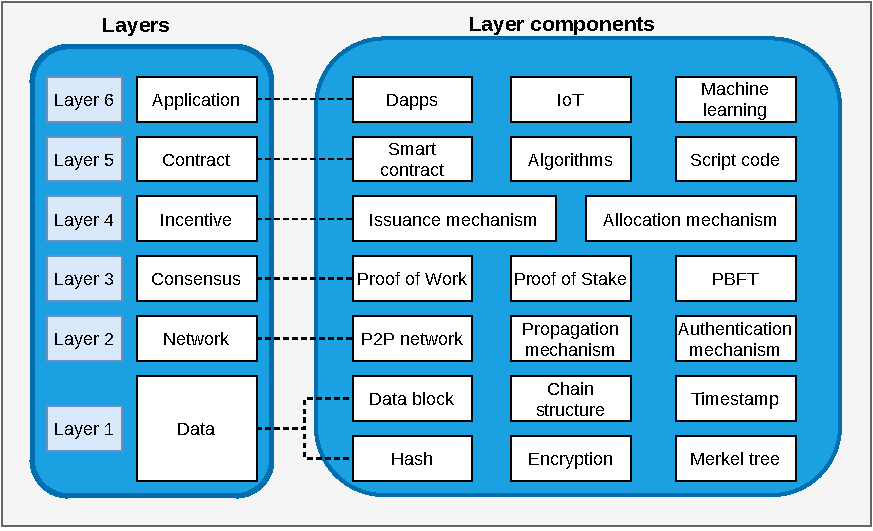
\includegraphics[width=\textwidth]{Images/layers.pdf}
\caption{Blockchain architecture in six layers, based on \cite{Yuan2018}} 
\label{F_layers}
\end{figure*}

The first \emph{data layer} involves the techniques required for storing transaction records. Each block in the ledger stores a set of verified, timestamped and hashed transactions, in the form of a Merkle tree \cite{Yuan2018, Issa2023}.

The \emph{network layer} (layer 2) includes the network aspects, such as the communication and verification mechanisms, including authentication. Nodes in a blockchain network usually interact forming a peer-to-peer (P2P) decentralized network. The network layer helps in broadcasting, forwarding and verifying transactions.  When a node creates a transaction, it signs it with its private key then broadcasts it to its neighbors. The neighbors verify this transaction with its public key. If the transaction is valid, it is added to the blockchain and broadcast to the other nodes of the network, or discarded otherwise \cite{Yuan2018, Issa2023}.

The \emph{consensus layer} (layer 3) is used by the network of nodes to reach an agreement on the state of the blockchain. The blockchain state includes the valid transactions, the blocks in the ledger and their order, as well as the next block to be added. Numerous consensus algorithms have been designed for blockchains, which are extensively discussed in Section \ref{ss_consensus_methods}.

The \emph{incentive layer} (layer 4) is a fundamental part of the blockchain architecture that encourages users to contribute to the network, usually with economic incentives.
The incentives are given to specific nodes so that they verify the blocks and keep the decentralized nature of the blockchain network. 

The \emph{contract layer} (layer 5) includes smart contracts, but also algorithms and script codes to extend the logic of transactions. This layer enables to devise more complex business rules, automatically performed when predetermined conditions are fulfilled.

The \emph{application layer} (layer 6) includes a wide range of applications that leverage blockchain properties. It can include generic applications, such as machine learning or the Internet of Things. Decentralized applications (DApps) are encompassed in this layer as well.

\begin{figure*}[t]
\centering
 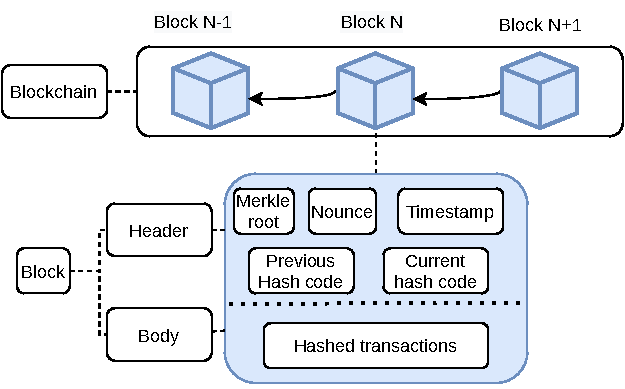
\includegraphics[width=0.7\textwidth]{Images/blockstruct.pdf}
\caption{Block composition - based on \cite{Issa2023}} 
\label{F_blockstruct}
\end{figure*}

\begin{samepage}
\textbf{Block composition.} \sul{The blocks composing the transaction ledger are composed of a header and a body, shown in Figure} \ref{F_blockstruct}. \sul{The body part of the block holds hashed transactions, while the header is constituted of these parts} \cite{Nakamoto2008, Issa2023}:

\begin{enumerate}

    \item \sul{\emph{Merkle Root}: The Merkle root is a hash value computed from the set of all transactions included in the block. It is used to cryptographically prove that all transactions within the block are valid and unchanged} \cite{Merkle87}.
    
    \item \sul{Nonce: a nonce is an arbitrary number that can be used just once in a cryptographic communication. Nonces are used in proof-of-work systems to vary the input to a cryptographic hash function to obtain a hash for a certain input that fulfills certain arbitrary conditions, notably on difficulty;} 
    
    \item \sul{Previous Hash Code: This field contains the hash value of the previous block in the blockchain. It forms the link between blocks and ensures the integrity and chronological order of the blockchain.}
    
    \item \sul{Timestamp: The timestamp indicates the exact time when the block was created. It provides a reference point for ordering blocks and contributes to the overall consensus mechanism of the blockchain.}
\end{enumerate}
    
\end{samepage}

\subsection{Consensus methods}
\label{ss_consensus_methods}

Consensus methods (layer 3, as introduced in Section \ref{S_distributed_ledgers}) are very diverse and have different advantages and drawbacks regarding performance, security and privacy. Due to their significant impact on the network characteristics, the most popular consensus mechanisms are discussed next.

\textbf{Proof of Work.}
The proof of work (PoW) is a consensus method based on a computation race. The first participant who solves the computation puzzle wins the right to add the next block to the transaction ledger.
 It was popularized by the Bitcoin blockchain as the first consensus method for blockchains \cite{Nakamoto2008}.
The user appending the new block to the ledger is called the \emph{miner}. The computation puzzle is most commonly based on a hash function, where the users have to find a nonce to solve the given problem.
 It consumes a lot of computational resources, raising environmental concerns \cite{Stoll2019, Sharma2023}.

Blockchain networks based on proof of work are vulnerable to the 51\% attack, which is a potential security vulnerability in blockchain networks where a single entity or group of entities gains control 
of more than 50\% of the network's mining power \cite{Aponte2021}. 
If an attacker gathers the majority of the mining power, it allows him to spend its funds multiple times, reorganize the blockchain by creating a longer chain with alternative transactions, or block the incoming transactions.

\textbf{Proof of Stake.} The proof of stake (PoS) was proposed to overcome the issues of the proof of work, in particular the high energy and computational resource consumption. In contrast with the proof of work, the PoS does not rely on a computation race but rather on an economic stake as proof to select the next validator.
The first cryptocurrency to use proof of stake is Peercoin (PPCoin)\cite{King2012}.
Ethereum, Bitcoin's main competitor, has replaced proof of work with proof of stake in its current version Ethereum 2.0. 
While proof of stake is not threatened by the 51\% attack\footnote{Yet, if a single entity or a group were to control the majority of the stake, they would have disproportionate influence over the network's consensus and decision-making process}, it is endangered by the \emph{Nothing at Stake} problem. 

The \emph{Nothing at Stake} problem arises when validators in a PoS network
 are not financially incentivized to follow the rules and behave honestly. Since validators do not have to spend computational resources or energy to create blocks in PoS, there is no direct cost associated with attempting to create multiple competing blockchains.
 This creates a scenario where validators can potentially create multiple valid chains in an attempt to double-spend or disrupt the network without any economic consequences. 
However, the \emph{Nothing at Stake} problem is not a practical vulnerability in most PoS protocols. This is because PoS protocols usually have mechanisms implemented to prevent or mitigate this problem. 
For example, penalties or slashing mechanisms can be used to punish validators who attempt to create multiple competing chains.

There are several variations of the proof of stake that are designed to adjust PoS performance metrics to fit specific use cases.
The \textbf{Delegated Proof of Stake} (DPoS) is a version of PoS where stakeholders vote to elect a set of delegates or validators who are responsible for producing blocks and maintaining the blockchain. These elected validators take turns creating blocks on behalf of the stakeholders who elected them.
The \textbf{Leased Proof of Stake} (LPoS) allows users to lease their stake or balance to a chosen delegate, who then includes their stake in their own validator's pool. This allows users with smaller stakes to participate in the block production \cite{Salimitari2020}.
The \textbf{Liquid Proof of Stake} (also LPoS) introduces a concept of liquidity, where stakeholders can freely transfer or trade their staked tokens while still participating in the consensus mechanism. This allows for more flexibility and liquidity compared to traditional staking mode \cite{Breitman2014}.

The \textbf{Proof of Authority} (PoA) is a variant of the proof of stake where the \emph{identities} and the \emph{reputation} of the nodes \emph{are at stake} rather than a cryptocurrency asset. The time to reach the consensus and the latency is better compared to the proof of work, but not as good as the actual proof of stake~\cite{Raghav2020}.
One significant contribution to its popularity was the introduction of the PoA consensus algorithm by Gavin Wood, the co-founder of Ethereum, in the Ethereum network's \emph{Parity} client \cite{Ekparinya2020}.
In the following, only the conventional PoS, the delegated and the proof of authority are considered, as both liquid and leased proofs do 
not have an impact on network metrics, but have an economic rationale.

\textbf{Proof of Elapsed Time.} In the Proof of Elapsed Time (PoET), the miner is chosen at random based on a timer. The user whose timer expires first becomes the miner. This consensus method has several benefits,
including a higher throughput and a low latency.
However, its main drawback is its reliance on Intel's SGX, as the correctness of the timer execution must be verified within a \emph{trusted execution environment}, implying PoET's governance is centralized.
 
The Proof of Elapsed Time consensus mechanism was popularized through its implementation in the Hyperledger Sawtooth blockchain platform, developed by the Linux Foundation. 
Intel, the company behind the creation of PoET, actively contributed to its promotion and adoption by highlighting its energy efficiency and scalability benefits compared to traditional consensus mechanisms like Proof of Work (PoW) \cite{NDSSWang2022}.

\textbf{Practical Byzantine Fault Tolerance.}
The Practical Byzantine Proof Tolerance (PBFT) is a voting-based consensus method. All the nodes are involved in the voting process and the consensus is reached when more than two-thirds of the nodes agree 
upon the next block. As a consequence, the network can handle malicious behavior from at most a third of the nodes, 
which is low compared to the 51\% assumption in the proof of work networks~\cite{Aponte2021}. PBFT is consequently efficient in private blockchains, but not for public blockchains which
have a lower tolerance to malicious nodes~\cite{Salimitari2020}. In addition, the voting process does not scale well, as PBFT generates a significant network 
overhead \cite{Salimitari2020}. 
Practical Byzantine Fault Tolerance (PBFT) was introduced by Miguel Castro and Barbara Liskov \cite{Castro1999}.
 The paper introduced the PBFT algorithm as a solution for achieving consensus in distributed systems under the presence of Byzantine faults.

A delegated version of the practical byzantine fault tolerance is used as well in cryptocurrencies called \emph{dPBFT}. dPBFT stands for \emph{Delegated Proof of Byzantine Fault Tolerance}. It is a consensus algorithm that builds upon the original PBFT algorithm. dPBFT was introduced to improve the scalability and performance of PBFT by allowing a smaller subset of nodes, known as \emph{delegates} or \emph{representatives}, to handle the consensus process on behalf of the entire network. This delegation reduces the communication and computational overhead compared to traditional PBFT, making it more suitable for large-scale distributed systems.
 dPBFT and the concept behind it have been popularized by the NEO cryptocurrency project, which implemented the dPBFT consensus algorithm as its underlying consensus mechanism \cite{Zhan2021}. 
\subsection{From blockchains to distributed ledgers}
\label{ss_blockchain_DLT}
 
 While blockchains are the most well-known instances of distributed ledgers for cryptocurrencies, the notion of \emph{Distributed Ledger Technology} (DLT) is broader and includes several other technologies of interest that are introduced in this section. 
 
 First, a distributed ledger can be completely disconnected from the notion of cryptocurrency, e.g., distributed databases. Besides, some cryptocurrencies do not build their transaction ledger using blockchains, but rather using different mathematical structures. The most used alternatives to blockchain in cryptocurrencies are the \emph{directed acyclic graphs} (DAGs) and the \emph{hashgraphs}.

  \begin{figure}
    \centering
    \begin{subfigure}[b]{0.48\textwidth}
        \centering
        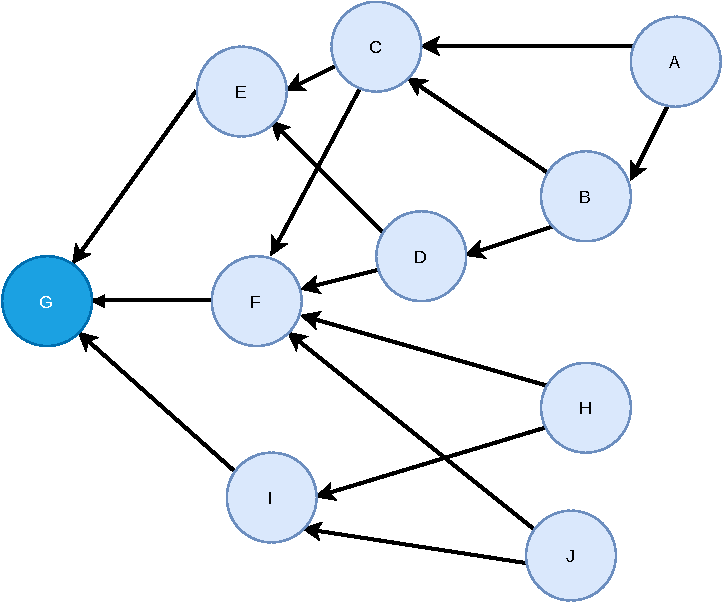
\includegraphics[width=0.8\textwidth]{Images/DAG.pdf}
        \caption{Directed acyclic graph (DAG). Transaction $A$ directly approves $B$ and $C$, indirectly approves $E$, $F$ and $G$. $G$ is the original transaction,
        approved by all other transactions \cite{Popov2017}.}
        \label{F_DAG}
    \end{subfigure}
    \hfill
    \begin{subfigure}[b]{0.38\textwidth}
        \centering
        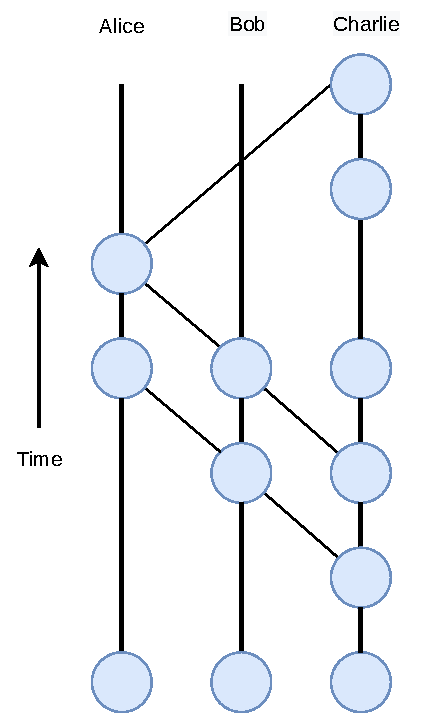
\includegraphics[width=0.63\textwidth]{Images/hashgraph.pdf}
        \caption{Hashgraph, representing the gossip history. If Alice receives gossip from Bob,
         the event is marked by a vertice in the Alice column, with two edges going downward
        to the preceding gossip events by Alice and Bob \cite{Baird2018}.}
        \label{F_hashgraph}
    \end{subfigure}
    \hfill

       \caption{Alternatives to blockchains to build transaction graphs.}
       \label{F_alternative_DLT}
\end{figure} 


 \textbf{Directed acyclic graph.} Unlike a traditional blockchain, where transactions are organized in linear blocks, a directed acyclic graph allows multiple transactions to be confirmed concurrently, 
 enabling greater scalability and potentially faster transaction processing times. Several cryptocurrencies rely on directed acyclic graphs to build the transaction ledger
 such as IOTA \cite{Popov2017}, Obyte~\cite{Churyumov2017} and Nano~\cite{LeMahieu2017}. IOTA is by far the most studied DAG-based distributed 
 ledger in the scientific literature \cite{Conti2022, Carelli2022, Guo2023, Naresh2023}.
 Though DAG-based technologies slightly differ, they share several interesting properties:
 \begin{itemize}
    \item small transactions fees, or even no transaction fees at all;
    \item writing transaction is not energy-intensive;
    \item throughput is high after the bootstrapping stage and increases with the number of users;
    \item users add their transactions directly to the network without relying on any intermediaries, such 
    as miners or gateways.
 \end{itemize}

In general, a DAG-based distributed network builds its transaction ledger as detailed next. The transactions
issued by nodes constitute the vertices of the transaction graph. There is only one transaction by vertice, in 
contrast with blockchains that usually store multiple transactions in one block. The edges of the graph are obtained as follows:
when a new transaction arrives, it must approve two previous transactions. These
approvals are represented by directed edges, as shown in Figure \ref{F_DAG}. If there are no
directed edges between two transactions $A$ and $B$, but there is a directed
path of length at least two from $A$ to $B$, we say that $A$ indirectly approves $B$.
There is an original transaction, which is approved directly or indirectly by all the transactions.
 
 \textbf{Hashgraph.} Hashgraph is a distributed ledger technology designed as an alternative to blockchains.
  The hashgraph technology is currently patented and used by the public ledger Hedera \cite{Baird2018}. Hashgraphs
  have been studied in the literature as possible alternatives to blockchains, in particular in the context 
  of the Internet of Things \cite{Bansal2020, Gao2022, Jha2022, Tarlan2022}. The claimed features of Hedera's hashgraph are the following:
  \begin{itemize}
    \item very high transaction throughput and low latency;
    \item \emph{fairness} in the ordering of transactions by using a consensus algorithm that considers the timestamp of each event.
     This approach aims to prevent unfair advantages or biases among participants, in particular in use cases involving real-time pricing such as stock markets;
     \item resilience against denial of service attacks thanks to asynchronous byzantine fault tolerance (aBFT) consensus. aBFT is 
     a version of PBFT for asynchronous networks; 
  \end{itemize} 

While these claims are attractive, Hedera's hashgraph lacks evaluation and peer review for the scientific community. 
In particular, the claim regarding throughput, up to 500.000 transactions per second \cite{Baird2018}, is way above the current
standards (24.000 TPS for Visa). Hedera claims that the network throughput is only limited by bandwidth, which requires each network 
node to be able to download and upload the transactions, which set high requirements on network nodes. Besides, the 
claims should be verified based on empirical evidence, performance benchmarks, and independent research.

\textbf{Hashgraph consensus protocol.} The core of the hashgraph consensus is called \emph{gossiping}. The gossip protocol unfolds as follows. 
The first member (Alice) chooses another member at random (Bob), and then Alice tells Bob all of the information she has about the current status 
of the ledger. Alice then repeats with a different
random member. Bob repeatedly does the same, as well as all other members of the 
network. Consequently, if a single member becomes aware of a new transaction, 
the information is spread exponentially fast through the community until every member is aware of
it.

In hashgraph, the participants do not only gossip transactions, but also the hashgraph itself, 
a process which is referred to as \emph{gossip about gossip}.
Gossiping a hashgraph gives the participants a great deal of information. 
If a new transaction is placed in the payload of an event, it will quickly spread to all
members, until every member knows it. A participant can learn about new transactions, know 
when exactly a participant learned about a given transaction, and also know
exactly when a participant learned the fact that another participant had learned of that transaction by transitivity.

The gossip history is therefore represented as a directed graph. The history of any
gossip protocol can be represented by a graph where each member
is a line composed of vertices. When Alice receives gossip from Bob,
telling her everything he knows, that gossip event is represented
by a vertex in Alice's line, with two edges going downward
to the immediately-preceding gossip events by Alice and Bob. 
The hashgraph is represented in Figure \ref{F_hashgraph}.

\subsection{Conclusion on distributed ledgers}

\sul{Distributed ledgers, whose most famous instances are blockchains, are in fact more diverse and encompass distributed databases as well as ledgers built using hashgraphs or directed acyclic graphs. Apart from the structure of the transaction graph, the main distinctive feature of distributed ledger is the consensus method, used to decide who can write the transactions and how. The consensus method has a strong impact on the network's security and performance, which we will discuss in Section} \ref{S_DLT_performance}. \sul{Besides, distributed ledgers are confronted to privacy challenges that are discussed in the next Section} \ref{S_privacy_DLT}

\section{Preserving privacy in distributed ledgers}
 \label{S_privacy_DLT}

While distributed ledger transactions are thought to be anonymous, the reality is more balanced. Public blockchains do not require identifying information to make a
transaction.  Yet, access to transactions and their content is not restricted. The transactions disclose information about the different parties involved and create risks of inference. Interested third parties also automatically collect and analyze
this information, for several purposes including law enforcement \cite{Harrigan2016}. By default, public blockchains only provide pseudonymity, or anonymity provided
the linkage between the pseudonym and the real identity is not possible. However, 
several behaviors drastically make re-identification easier, which are discussed in the section \ref{ss_de_anonymisation}.
In the next section, we detail the privacy threats for distributed ledger technology, based on LINDDUN privacy threat modeling \cite{Wuyts2015}.

\subsection{Privacy threat modeling.}
\label{ss_privacy_threat_modeling}
LINDDUN is a privacy threat modeling framework \cite{Wuyts2015} to reason about potential privacy concerns in 
a systematic and structured way. It is structured according to seven threat types captured in the 
acronym LINDDUN. LINDDUN is used in this section to identify the main privacy threats in distributed ledgers 
so that the risks addressed by the privacy-preserving tools detailed in the following (Section \ref{ss_obfuscation_coin_mixing_merge_avoidance})
are clearly expressed.

\textbf{Linking.} Linking is the association of data items or user actions to learn more about an 
individual or a group. In blockchains, linking threats can be done by linking several transactions 
together to deduce the consumption habits of a user, or by linking senders and receivers of transactions.

\textbf{Identifying.} The identifying threat is the risk of learning the identity of an individual, even though 
it wants to remain anonymous. In distributed ledger technologies, the main risk is breaking the pseudonym, i.e., the 
address of a user in the blockchain, to disclose its true identity. This is usually achievable 
by combining blockchain data with external information, such as network data, by identifying 
from which IP address a transaction originates.

\textbf{Non repudiation.} The non-repudiation threat is the ability to attribute a claim to an individual, e.g., read a message. 
The system maintains evidence regarding some actions of facts, which implies deniability claims, like log files or metadata. 
Non-repudiation is a counter-intuitive notion when it comes to privacy threat assessment, as 
in \emph{security threat modeling} such as STRIDE \cite{Howard2006}, repudiation is conversely 
considered as the security risk. In security, it is more relevant to prevent a malicious user 
from denying it performed a forbidden action, while for privacy preservation, it is better 
to be unable to attribute actions to individuals. An example of non-repudiation risk 
for a blockchain user is the impossibility to deny it performed a transaction.

\textbf{Detecting.} Detecting is the ability to deduce the involvement of an individual through observation. 
Notably, as the ledger is public, it is possible to see if a user made transactions in a blockchain 
network as its address is recorded in the transaction. It is an issue when combined 
with identification attacks, or if the motive of the transaction can be disclosed.

\textbf{Data disclosure.} Data disclosure is the excessive collection, storage, processing or sharing of personal data.
This is not a general threat in blockchains and distributed ledger technologies and is rather implementation-dependent.

\textbf{Unawareness.} Unawareness corresponds to insufficient information and involvement of individuals in the 
processing of their personal data. It is also not a general risk.

\textbf{Non-compliance.} The last non-compliance threat reflects the deviation from security and data management best practices, 
standards, and legislation. Distributed ledger technologies can be legal conundrums regarding
 the EU General Data Protection Regulation (GDPR) \cite{EUdataregulations2018, Haque2021}:
\begin{enumerate}
    \item Article 3 - \emph{Territorial scope}. Article 3 is about
    controlling the user data from being processed and stored outside 
    the geographical area of the EU. In the case of the public blockchain, it is difficult since
    the nodes are distributed worldwide. Private blockchains can conversely have nodes 
    that are located in the same region;
    \item Article 16 and 17 - \emph{Right to deletion and modification}. 
    One of the most important legal issues for blockchains 
    is Article 17 of GDPR,
    about the \emph{right to be forgotten}. That means the concerned
    organizations should delete the user data if the users request it. 
    Since information inside the blockchain cannot be
    removed, it directly contradicts Article 17.
    This is also true for Article 16 \emph{right to rectification} as data cannot be edited either.
    \item Article 4 states the definition of \emph{personal data}, data \emph{controller},
    and data \emph{processors}. Articles 24 and
    28 describe data controllers’ and processors’ purposes and
    responsibilities. Identifying data controllers and processors is hard for blockchains since no centralized authority is
    controlling the nodes or is accountable for them.
\end{enumerate}



\subsection{Breaking pseudonymity in blockchains}
\label{ss_de_anonymisation}

Most public blockchains including the two most popular, Bitcoin and Ethereum, only provide pseudonymity under the form of an address. Anonymity would be provided if it is not possible to link the pseudonym and the real identity. However, several behaviors of users and techniques significantly ease the re-identification process.

\textbf{Clustering.} Address clustering in the context of blockchain refers to the process of identifying multiple addresses that belong to the same user or entity by analyzing their transactional behavior on the blockchain \cite{Huang2017}. It is a method used to de-anonymize blockchain transactions and can potentially reveal the identity of the user or entity behind the transactions. Address clustering is a common technique used by law enforcement \cite{Harrigan2016} agencies to investigate illicit activities such as money laundering and terrorist financing.

\textbf{Address reuse.} Address reuse in blockchains occurs when the same public address is used for multiple transactions. This can be problematic for several reasons. First, for privacy, when a user reuses an address for multiple transactions, it becomes easier for anyone to track the user's transactions as it requires to link one address to an identity. Conversely, using a different address for each transaction requires repeating the process of re-identification several times, which is time-consuming. Additionally, address reuse is a problem for security, as the leak of only one private key enables a malicious agent to steal all the funds of a user.

\textbf{Network analysis.}  By monitoring network traffic and analyzing the timing, size and value of transactions, it is possible to infer relationships between addresses and potentially identify the real-world identities hidden behind the 
pseudonym address. For instance, heuristics have been developed to identify ownership relationships between Bitcoin addresses and IP addresses \cite{Koshy2014},
significantly facilitating re-identification.

\subsection{Obfuscation using coin mixing and merge avoidance}
\label{ss_obfuscation_coin_mixing_merge_avoidance}
Coin mixing services allow users to mix cryptocurrency coins
to enable unlinkable payments and prevent tracking of honest users’ coins by both the service provider i.e. the \emph{coin mixer} or \emph{coin tumbler}, and the users themselves.
The easy bootstrapping of new users and backward
compatibility with cryptocurrencies are attractive features of this service, which
has recently drawn the attention of both academia and
industry. While useful for privacy preservation, coin mixers face several technical challenges such as decentralization to be able to meet their requirements as regards privacy.

\textbf{Principles of coin mixing.} Cryptocurrency mixing services are designed to remove the linkage between senders and receivers of transactions. To achieve this task, the cryptocurrency mixing service gathers coins from different users, whose identities are linked to these coins. The mixing service then keeps the coins for a random time before assigning the coins to the users. The coins are distributed at random which removes the linkability between the coins and the users. The purpose of randomness and keeping the coins for a long time is to avoid the re-identification of the sender by using timestamps. The mixing process is shown in Figure \ref{F_coin_mixing}.
Mixing services should have the following guarantees:

\begin{itemize}
    \item \emph{anonymity}: usually considered as the unlinkability between the senders and the receivers of the transactions \cite{Sarfraz2019, Seres2019, Glaeser2022};
    \item \emph{availability}: users must be able to withdraw their cryptocurrencies from the mixer \cite{Seres2019};
    \item \emph{correctness}: no malicious participant should be able to steal other participants' cryptocurrencies \cite{Sarfraz2019, Seres2019}, or their private keys including partial private keys \cite{Sarfraz2019};

\end{itemize}
\begin{figure*}[t]
\centering
 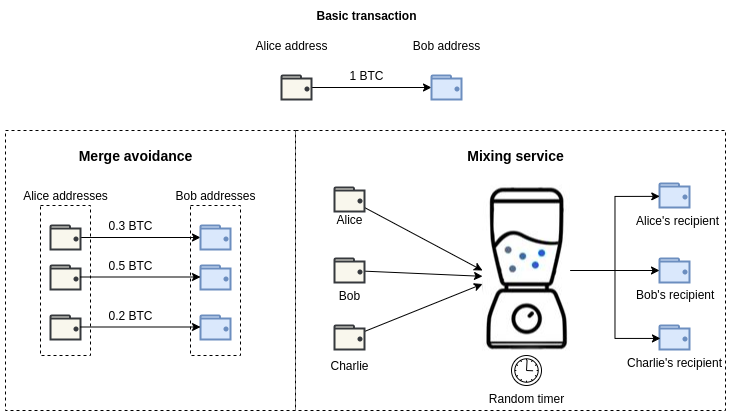
\includegraphics[width=\textwidth]{Images/mixing_merge.png}
\caption{Coin mixing and merge avoidance for transaction obfuscation.} 
\label{F_coin_mixing}
\end{figure*}

\textbf{Limitations of centralized coin mixing.} Centralized coin mixing services, although important privacy-enhancing parts in blockchains have several limitations which create significant risks for users:
\begin{itemize}
    \item \emph{availability}: being centralized and responsible for obfuscating transactions, coin mixing services are likely targets of denial-of-service attacks as single points of failure (SPOF) \cite{Sarfraz2019};
    \item \emph{trust}: the centralized mixing service needs to be trusted, as it still can link the sender and the receiver of the transaction, and also can keep the coins for itself, or take a fee without actually providing the service.
\end{itemize}

These two limitations are direct risks to the security and privacy of the users. This justifies the introduction of decentralized mixing schemes.

\textbf{Decentralized coin mixing.}
Coin mixing services, when centralized, become a single point of failure \cite{Sarfraz2019, Andola2021} and are targets of choice for attackers willing to break the privacy of users or to embezzle the coins. Therefore, the first natural step to improve coin mixing would be to decentralize the mixing service. Decentralized mixing faces a major issue nonetheless, known as the \emph{bootstrapping problem}\cite{Glaeser2022}. The bootstrapping problem is the difficulty to find a set of initial participants to execute the protocol.
While a high number of participants is desirable to improve
the anonymity guarantees provided by the coin mixing protocol, it is at the same time undesirable as it results in
poor scalability and makes bootstrapping harder \cite{Glaeser2022}. 

While decentralized mixing services are more resilient against denial of service attacks, the decentralization 
is troublesome as well as it exposes the mixing service to \emph{edge insertion attacks}.
In such attacks, a malicious user claims that additional mock nodes were involved in the mixing process to receive the corresponding rewards on their behalf \cite{Simoes2021}. While this kind of attack is easy to mitigate with a central entity accountable for node identity verification,
it becomes a challenge in a distributed setting. This attack is hard to prevent in distributed ledgers with transaction fees, as the miner, and consequently, the mixing service must be 
paid to fulfill their role and cover their costs.

\textbf{Merge avoidance.}
Merge avoidance is a technique first designed for Bitcoin \cite{Hearn2013, Simoes2021} by Mike Hearn, a Bitcoin developer, but it can be generalized to other cryptocurrencies \cite{Sarfraz2019}. In merge avoidance, a single transaction between two users is split into numerous sub-transactions for both users, hiding the amount of the original transaction. A new address must be created for each sub-transaction, and the addresses must not be linked to the identity of the sender. Otherwise, it will be easy to rebuild the original transaction using a blockchain explorer with either the sender or the receiver address.

The purpose of merge avoidance is to prevent inference attacks, in which an attacker could use the amount of cryptocurrency sent to infer the purpose of the transaction. For instance, let's consider a case where Alice is getting paid her wage in the Ethereum cryptocurrency (ETH). Each month, she gets her wage to the same wallet, at a similar time of the month. An attacker can easily guess the purpose of the transaction by observing the different transactions with Alice's wallet as outputs. By sending each individual wage in different sub-transactions to multiple wallets belonging to Alice, it is much harder to identify the purpose of the payments.
However, the merge avoidance strategy has downsides \cite{Hearn2013}:

\begin{itemize}
    \item as a receiver, your level of privacy depends on the sender and how it crafts transactions. However, the senders do not have a strong incentive to protect your privacy and may just ignore the merge avoidance process if it is not compulsory;  
    \item it increases the number of transactions, which increases the size of the ledger, but the overhead is quite limited \cite{Hearn2013};
\end{itemize}

\subsection{Privacy-oriented cryptocurrencies}

While privacy-enhancing technologies have been devised to preserve the privacy of blockchain users, other cryptocurrencies endeavor to implement privacy by design. Here are a few technologies of interest focusing on privacy protection:

\textbf{Monero} (XMR): Monero \cite{Saberhagen2013} is a privacy-focused cryptocurrency that uses a technology called \emph{ring signatures} to mask the sender's identity. It relies on stealth addresses to conceal the recipient's address and \emph{ring confidential transactions} (RingCT) to obfuscate the transaction amount. These techniques make it difficult to trace Monero transactions and provide a high level of privacy.

\textbf{Zcash} (ZEC): Zcash \cite{Bowe2016} is a privacy-oriented cryptocurrency that uses a technology called \emph{zero-knowledge proofs} (ZKPs) to keep transactions private. ZKPs allow users to prove that a statement is true without revealing any additional information beyond what is necessary \cite{Goldwasser1985}. In Zcash, ZKPs are used to hide transaction details such as the sender's address, the recipient's address, and the transaction amount.

\textbf{Dash} (DASH): Dash \cite{Duffield2014}is a privacy-focused cryptocurrency that offers optional privacy features. Dash seeks to improve upon Bitcoin (BTC) by providing stronger privacy and faster transactions. Its \emph{PrivateSend} feature allows users to mix their transactions with other users to make them more difficult to trace. PrivateSend uses a decentralized network of \emph{masternodes} to mix transactions, ensuring that no single entity can track the transaction history.

\subsection{Conclusion on privacy}
\label{ss_conclusion_on_privacy}

While blockchain transactions are often considered privacy-preserving, distributed led/- gers are confronted with challenges when protecting users' anonymity. Distributed ledgers often only provide pseudonymity, which can be broken by some actors notably by using network information. Some privacy-enhancing technologies have been designed to safeguard users' anonymity, such as the coin mixer, whose purpose is to prevent the linkage between the sender and the receiver of a transaction. Additionally, some cryptocurrencies have been designed to specifically provide anonymous transactions (ZCash, Monero...). In the next section, we will discuss the performance aspects of DLT, such as the metrics used to describe the performance of a distributed ledger, as well as the impact of the consensus methods on these metrics. 
\section{Performance considerations of distributed ledger technologies}
\label{S_DLT_performance}

Due to resource-consuming and time-consuming consensus methods, blockchains and distributed ledger performances have been critically important in the literature. \cite{Brotsis2021, Fan2021, Chen2022, Okegbile2022}. 
Performance aspects are the basis used to compare consensus methods and suggest or preclude the use of a consensus method for a use case. In this section, we will first introduce the metrics used to assess the performance of a consensus method (Section \ref{ss_performance_metrics}), before detailing the expected performance of the most important methods and how they answer the Internet of Things requirements (Section \ref{ss_performance_consensus_methods}). 

% Finally, in Section \ref{ss_suitability_iot}, the suitability of the distributed ledgers for the Internet of Things is assessed, based on their expected performance.

\subsection{Performance metrics}
\label{ss_performance_metrics}

To assess the performance of distributed ledger technologies, a wide range of parameters can be considered. Security aspects must also be considered as increasing performance may impact security negatively. In distributed ledger technologies, this translates into a relatively low adversary tolerance. \emph{Adversary tolerance} is achieved through designing consensus protocols that guarantee security even in the presence of an adversary who may control up to a certain fraction of the resources of the system. This fraction expresses the robustness of the consensus method. We now look at the different metrics used to measure the performance of a consensus method.

\textbf{Throughput}, or in the context of distributed ledger, transaction throughput, is the number of transactions that a blockchain network can process per unit of time. It is usually expressed in \emph{transaction per second} (TPS). It must be distinguished from \emph{network throughput}, which measures the amount of data that can be transmitted from one point to another within a given time. It is usually expressed in bits per second (bps) or bytes per second (Bps) but is a less relevant notion for blockchain networks. Transaction throughput can greatly vary when comparing DLTs. The Bitcoin blockchain has a maximum throughput of around 3-7 transactions per second, while Ethereum, the $2^{nd}$ most important blockchain in capitalization has a throughput between 15 and 45 TPS in its current version \footnote{Ethereum 2.0 is expected to drastically increase the throughput}. Compared with traditional payment networks, Visa can process up to 24.000 transactions per second, while Paypal has a 193 TPS throughput. A final thing to consider when discussing throughput is the range. A network processing under 100 transactions per second can be considered as having a low throughput, while 100 to 1000 TPS will be considered average and over 100 TPS a high throughput \cite{Salimitari2020}.

\textbf{Latency}, in blockchain networks, is the amount of time between initiating a transaction or payment and receiving confirmation that it is valid \cite{Kokoris-Kogias2022}. It is sometimes referred to as \emph{block time}, which covers a slightly different notion as blocks are not transactions, but groups of transactions. For instance, a block of the Bitcoin blockchain can be made of 2000 transactions \cite{nasdaq2023}. Latency is usually expressed in seconds.
While latency may seem to be the inverse of throughput, these two notions are not related. Indeed, when the system is at a low load, the number of transactions per second can increase until reaching the high load regime for the network, with no impact on the latency. Conversely, on high load, if new transactions are pushed to the network, the throughput stays the maximum, but the latency keeps on increasing. Both notions are therefore necessary to reflect the transaction processing capacity of a given distributed ledger network. 

\textbf{Scalability}, which actually covers two different concepts~\cite{Steen2020}. First, scalability in terms of transaction processing capacity, and can be considered as throughput. Then, scalability in terms of the number of users, which is positively impacted by the open membership, the lack of any centralized component and the absence of trust assumptions on any third-party~\cite{Steen2020}. Scalability is consequently strongly related to decentralization. As set in assumptions (cf. Section \ref{S_assumptions}), only large-scale IoT networks are considered in this thesis, which implies that high scalability is compulsory. Despite being crucial, it is also one of the most difficult metrics to evaluate accurately.

\textbf{Network overhead}.
In the context of distributed ledgers, network overhead refers to the amount of additional data transmitted over the network that is required to support the consensus protocol, verify transactions, or maintain the distributed ledger system. This additional data can include message headers, authentication and encryption data, transaction data, and consensus-related data, and can increase the total amount of network traffic required to operate the system. This is a metric of interest for the Internet of Things, as a high network overhead will limit the scalability in terms of nodes.

\textbf{Storage overhead} is the additional storage space required to maintain the ledger, including transaction data and metadata, on each node in the network. Internet of Things devices e.g., sensors, may have very low storage. A high storage overhead excludes low storage devices from contributing to the consensus method.
\rul{Additionally, devices must store basic knowledge of the network even though they do not contribute to the network as a node. In particular, devices need to store network configuration information to connect to the network. This includes details such as the IP addresses and ports of nodes it will communicate with.  Each IoT device should also store its private keys associated with its addresses. The private keys allow the device to sign transactions and prove ownership of the associated addresses and coins.}
\subsection{Performance of consensus methods}
\label{ss_performance_consensus_methods}

Using the above-mentioned performance metrics (cf. Section \ref{ss_performance_metrics}), we discuss how consensus methods compare with each other. In particular, we highlight which distributed ledger technologies are suitable for the Internet of Things from a performance perspective, i.e., regardless of security and privacy concerns. The discussion is summarized in Table \ref{tab:performance_dlt}.

\textbf{Proof of Work.} The PoW is a consensus method based on a computation-intensive cryptographic puzzle. The difficulty of the cryptographic challenge directly defines the security and the performance of the network. By design, PoW-based blockchains usually have a low throughput and a high latency to allow time for the nodes to check the new transactions' correctness. Storage is troublesome as well, as the size of the ledger is continuously increasing and can not be stored on a device with low capacity. PoW is consequently not adapted for the Internet of Things.

\textbf{Proof of Stake.} The proof of stake removes the computation race between nodes, alleviating computation requirements compared to the proof of work. However, throughput is still low considering IoT requirements \cite{Raghav2020}. As it is a monetary-based approach, it is often excluded for IoT use cases \cite{Raghav2020, Salimitari2020}, as it requires constrained devices to hold a cryptocurrency. The proof of stake also tends to concentrate the power into the hands of the richest nodes, centralizing the network to some extent \cite{Salimitari2020}. The \textbf{Proof of Authority} is very similar to the proof of stake but does not introduce monetary concepts.

\textbf{Delegated Proof of Stake.} Electing miners and nodes responsible for the network management significantly improves throughput and latency, but centralizes the network. Besides, it also requires holding a cryptocurrency to participate in the voting, limiting its adoption in the Internet of Things.

\textbf{Proof of Elapsed Time.} The proof of elapsed time has a low latency and a high throughput and can be considered IoT-friendly \cite{Salimitari2020}. The only drawback is the need to verify the timer's execution using a dedicated \emph{Trusted Execution Environment}. For PoET, it is usually done using Intel's SGX software, which makes it partly centralized and limits its use in large-scale networks.

\textbf{Practical Byzantine Fault Tolerance.} Similarly to PoET, PBFT features high throughput, low latency and low computational overhead making it appealing for IoT networks. However, PBFT requires a lot of messages to achieve consensus and has a high network overhead, strongly limiting its scalability and restricting its use to private blockchains and small IoT networks. The \textbf{delegated Byzantine Fault Tolerance} does not require the participation of all nodes in the consensus, aiming at solving the network overhead issue, but at the cost of higher latency making it unsuitable for the Internet of Things \cite{Salimitari2020}.

\textbf{IOTA.} IOTA has been specifically designed for the Internet of Things requirements. IOTA provides high throughput and low latency for transactions, as well as high scalability \cite{Alshaikhli2022}. Nodes do not require to store the whole ledger to run, rather relying on automated snapshotting, limiting storage overhead. \rul{IOTA is introduced in detail in Chapter} \ref{C_solving_trilemma} (Section \ref{S_iota_dlt})\rul{ and is identified as a crucial technology for the Internet of Things.}
\begin{table*}
\begin{center}
 \begin{scriptsize}
\setlength{\extrarowheight}{12pt}
\begin{adjustbox}{angle=90}
\begin{tabular}{ |c|c|c|c|c|c|c|c|c|} 
\hline
Consensus method & Scalability & Latency & Throughput & Adversary tolerance & Network overhead & Storage overhead & IoT suitable\\
\hline
PoW & High & High & Low  & <51\% computing power & Low & High & \xmark \\ 

PoS & High & Medium & Low & <51\% stakes & Low & High & ?\\ 

PoA & High & Medium & Low & <51\% stakes & Low & High & ?\\

DPoS & High & Medium & High & <51\% validators & n/a & High & ?\\

PoET & High & Low & High & n/a & Low & High & \cmark (small scale)\\

PBFT & Low & Low & High & <33\% faulty replicas & High & High & \cmark (small scale)\\ 

dBFT & High & Medium & High & <33\% faulty replicas & High & High & \xmark\\ 

IOTA & High & Low & High & <33\% computing power & Low & Low & \cmark\\ 

\hline

\end{tabular}
\end{adjustbox}
\captionof{table}{Performance of consensus methods - based on \cite{Salimitari2020}}
\label{tab:performance_dlt}
 \end{scriptsize}
\end{center}
\end{table*}


\section{Conclusion}
\label{S_conclusion_state_of_the_art}
In this chapter, we introduced the state of the art on usage control and on distributed ledger technologies needed to understand the context and the contributions of this 
thesis. First, we highlighted the purpose of usage control and information flow control to monitor data usage and data dissemination (Section \ref{S_usage_control}). Then, distributed ledger 
technologies have been extensively discussed, from general considerations (Section \ref{ss_DLT_elementaries}) to privacy challenges (Section \ref{S_privacy_DLT}). Finally,
we addressed performance aspects of distributed ledgers, which are paramount considering Internet of Things constraints. The performance of 
a distributed ledger technology is deeply correlated to the method used to achieve consensus.

In the following chapters, the different contributions of this thesis are described. The next chapter \ref{C_solving_trilemma} introduces a framework for efficient, privacy-preserving zero-fee transactions in the Internet of Things (\hyperref[obj:1]{\emph{Objective 1}}).
The framework is based on the aforementioned technologies, notably usage control, distributed ledgers and privacy-enhancing technologies 
for transactions, motivating this chapter on the state of the art and its analysis.

\newpage \ \newpage
%-------------------------------------------------------------------------------
%\chapter[A Framework for Performance, Security and Privacy in the Internet of Things]{\rul{A Framework for Enhancing Performance, Security, and Privacy in the Internet of Things}}

\chapter{\rul{A Framework for Enhancing Performance, Security, and Privacy in the Internet of Things}}
\label{C_solving_trilemma}
\minitoc


In the context of the Internet of Things, as defined in Section \ref{S_assumptions}, a framework for zero-fee transactions in the Internet of Things (\hyperref[obj:1]{\emph{Objective 1}}) should consider transactions to be granted access to physical devices
, e.g., cars and doors, but also to the data generated by the devices, as those data are valuable.
To this end, we will focus in this chapter on designing a framework that:

\begin{itemize}
  \item provides access control on physical devices and goods; 
  \item provides access and usage control on data; 
  \item has no fee, or very low fees, to enable micro-transactions;
  \item preserves the privacy of both participants of a transaction;
  \item considers the performance and the security requirements of the Internet of Things.
\end{itemize}

This chapter is structured as follows. First, the IOTA technology, a distributed ledger with zero-fee transactions is introduced in Section \ref{S_iota_dlt}. IOTA uses a DAG to build its transaction graph 
(cf. Section \ref{ss_blockchain_DLT}), and was designed to answer the performance requirements of the Internet of Things. IOTA is the key technology of the 
framework, from which the other tools are derived. Then, the framework and its components are detailed in Section \ref{S_framework}. Finally, a security and privacy threat assessment is conducted in Section \ref{S_security_and_privacy_evaluation}.
A conclusion of the chapter is provided in Section \ref{S_conclusion_ifip}.

\section{IOTA distributed ledger}
\label{S_iota_dlt}
In this section, we introduce IOTA as a key technology of the proposed framework, since most of the tools presented 
are derived or adapted to this distributed ledger.
As discussed in Section \ref{S_DLT_performance}, blockchain technology has several security and performance drawbacks 
for the Internet of Things which limits its 
adoption. Besides, transaction fees in some public blockchains can 
be greater than the actual transaction value, making micro-transactions impossible. Removing transaction fees in blockchains 
is an intricate issue since transaction
fees are used as an incentive for creators of blocks to contribute to the network. These different issues justify the need 
to introduce a new paradigm for 
cryptocurrency transactions. 

\subsection{\rul{Identifying DAG-based distributed ledgers for Internet of Things performance}}

 \rul{As part of the second research objective} (\hyperref[obj:23]{\emph{Objective 2}}), \rul{it is necessary to identify the most suitable distributed ledger technology for the Internet of Things. Distributed ledger technologies are interesting in the first place, due to the partial decentralization they provide and due to the immutability of the ledger which is useful for several applications, e.g., trust management, secure and private transactions (cf. Section} \ref{ss_motivation}). 

 \rul{In the state of the art} (Chapter \ref{C_state_of_the_art}), \rul{we introduced different criteria to differentiate distributed ledgers: consensus methods, performance metrics or the nature of the transaction ledger. In particular, distributed ledgers based on a directed acyclic graph or the Hashgraph have very attractive metrics. In theory, they both provide high throughput, i.e., numerous transactions per second, which is not often the case for blockchain-based distributed ledgers.}

 \rul{Yet, directed acyclic graphs are a better alternative as:}

 \begin{enumerate}
   \item DAGs are permissionless ledgers\footnote{It is although possible to deploy private instances of directed acyclic graphs, cf. Section \ref{ss_testbed}} in contrast to Hashgraph, and provide a higher degree of decentralization;
   \item Hashgraph is a project poorly studied by academia while DAGs, in particular IOTA, are being increasingly studied by the research community;
   \item the bandwidth requirements of Hedera's Hashgraph set a high barrier to entry for nodes, limiting its adoption for the Internet of Things. Nodes require at least 256 GB of RAM and 24-core or better CPU hyperthreaded (48 threads) as a minimum.
 \end{enumerate}

\rul{If distributed ledgers using a directed acyclic graph for their transaction ledger are suitable for the Internet of Things, the choice of IOTA rather than other DAG technologies, e.g., Obyte or Nano, is further motivated in Section} \ref{ss_benefits_iota}.

\subsection{A DAG-based transaction ledger}
IOTA builds its transaction graph using a directed acyclic graph (cf. Section \ref{ss_blockchain_DLT}) called the \emph{Tangle}. The difference between the tangle and a blockchain is represented in Figure \ref{F_dag_vs_blockchain}.
IOTA has properties common to DAG-based distributed ledgers, i.e., low transaction fees, disintermediation, and high throughput.
As a reminder of Section \ref{ss_blockchain_DLT}, transactions in a network based on a directed acyclic graph are built as follows. 
The transactions are the vertices of the transaction graph. There is only one transaction by vertice.
When a new transaction arrives, it must approve two previous transactions. The approval is materialized by an edge. These
approvals are represented by directed edges. If there are no
directed edges between two transactions $A$ and $B$, but there is a directed
path of length at least two from $A$ to $B$, we say that $A$ indirectly approves $B$.
There is an original transaction, which is approved directly or indirectly by all the transactions, called \emph{the Genesis transaction} 
in IOTA. 

The genesis is described in the following way. At
the beginning of the tangle, there was a single address with a balance that contained all
IOTA tokens. The Genesis transaction sent these tokens to several other addresses belonging to the founders. All of the tokens were created in the genesis transaction and as there is no mining, it is impossible 
to create iota tokens without \emph{taint}.
A token is considered tainted if it belongs to at least one identifying address on the IOTA ledger. 
Only iotas that have never been linked to any identifiable address, i.e. an address belonging to someone who has been re-identified, can be considered as untainted~\cite{Tennant2017}.

Finally, for a transaction site on the IOTA ledger, there is an associated \emph{weight} $w$. The general idea behind this notion is that 
a transaction with a significant weight is more important and trusted. Along weight, the notion of \emph{cumulative weight} $w_{cum}$ of a transaction $t$
 is also introduced, as the sum of its weight plus the weight of all transactions validating (including indirectly)  the transaction $t$.
 In Figure \ref{F_dag_vs_blockchain}, both weights and cumulative weights (respectively $w$ and $w_{cum}$) are given inside the sites of the DAG.
 For instance, the transaction $F$ has a weight $w_F = 2 $, is directly validated by $B$ and $E$ and indirectly by $A,C,$ and $D$. 
 Therefore, the cumulative weight of $F$ is $w_{cum,F}= (w_A + w_B + w_C + w_D + w_E) + w_F = 1+1+1+1+4+2 = 10$.  
\begin{figure*}[t]
\centering
 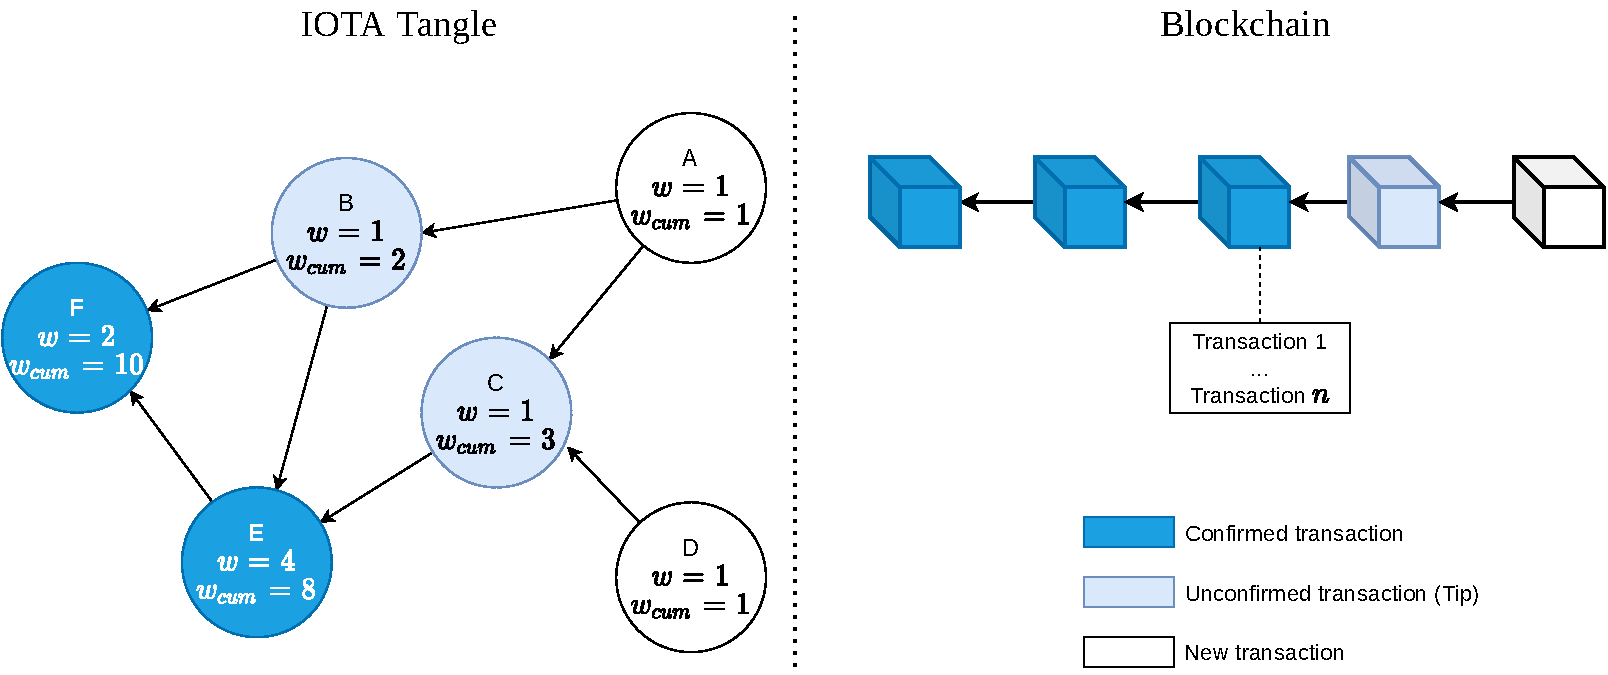
\includegraphics[width=\textwidth]{Images/IOTA_vs_blockchain.pdf}
\caption{Transaction ledger in the Tangle (directed acyclic graph) and a blockchain. Each transaction site on the DAG has a weight $w$ and an indirect 
cumulative weight $w_{cum}$}
\label{F_dag_vs_blockchain}
\end{figure*}

\subsection{Consensus method}
\label{ss_consensus_method}

In IOTA, to issue a transaction, users must
work to approve other transactions, so that users themselves are
contributing to the network’s security. The nodes check in particular if the
approved transactions are not conflicting. If a node finds a transaction conflicting with the tangle history, the node will not approve the conflicting transaction
directly or indirectly. In case a node issues a new transaction that validates conflicting transactions, it is at risk that other
IOTA nodes do not approve its transaction. As a transaction receives additional approvals, i.e., its weight is increasing, it 
gets a higher level of confidence. It consequently becomes harder for the system
to accept double-spending transactions.

A new transaction, i.e., not approved by other transactions, in the IOTA network, is called a \emph{tip}. To issue a new transaction, an IOTA node proceeds to the following steps:

\begin{itemize}
  \item The node picks two other transactions to approve according to a \emph{tip selection algorithm} (TSA);
  \item The node checks if the two transactions are conflicting;
  \item The node solves a cryptographic challenge to prevent spam. It works exactly like Bitcoin's proof of work, 
  but the challenge is not designed to pick the next miner, but only to make sure a node can not spam the network 
  by pushing too many transactions simultaneously.
\end{itemize}

The IOTA network is asynchronous, which means that the tangle may contain conflicting transactions. However, the nodes \emph{do not 
have to achieve consensus} on which transactions are valid and should be in the tangle, which is a significant difference with blockchains. 
That implies that all the transactions can be in the ledger. However, if there are two conflicting transactions, the nodes 
have to decide which transaction will be \emph{orphaned}, i.e., not validated indirectly by new transactions.

\textbf{Tip selection algorithm.}
In IOTA, the tip selection algorithm (TSA) determines which tips should be approved and referenced in new transactions.
 It aims to achieve a balance between security and network efficiency.
The tip selection algorithm in IOTA is based on a \emph{Monte Carlo Markov Chain} (MCMC).
The MCMC algorithm takes into account various factors such as the cumulative weight of transactions, 
the transaction arrival rate, and the network topology. By considering these factors,
 the algorithm selects tips that are more likely to be included by other transactions in the Tangle, 
 increasing the chances of approval for the users and overall transaction confirmation.
The tip selection algorithm plays a crucial role in the security and performance of the IOTA network. It helps prevent the concentration of approvals on a single branch of the Tangle,
 improving the resilience against potential attacks. 
Additionally, the algorithm aims to maintain a balanced distribution of transaction approvals across the network,
 ensuring efficient propagation and confirmation of transactions.

 \subsection{Benefits of IOTA}
\label{ss_benefits_iota}
 IOTA is a DAG-based distributed ledger and therefore has the attractive features of this technology. These benefits have been listed in Section \ref{ss_blockchain_DLT} and are the following:

 \begin{itemize}
  \item writing transaction is not energy-intensive, enabling low-power devices to participate in the network;
  \item throughput is high after the bootstrapping stage and increases with the number of users;
  \item users add their transactions directly to the network without relying on any intermediaries, such as miners or gateways.
\end{itemize}

In particular, the high throughput answers the scalability requirements of large-scale networks (cf. Section \ref{S_assumptions}) as it enables to process the high volume of transactions. In addition, IOTA does not have any transaction fee due to the removal of miners (\hyperref[obj:1]{\emph{Objective 1}}), while other distributed ledgers using a DAG have small fees \cite{Churyumov2017, LeMahieu2017}. IOTA is also largely studied and used in the literature \cite{Alshaikhli2022, Conti2022, Guo2023, Alsadi2023}, and the IOTA foundation, the main actor supporting the development of IOTA, also contributes to the scientific literature\footnote{https://www.iota.org/foundation/research-papers}. Finally, IOTA is built to be resistant to an adversary with a quantum computer \cite{Popov2017}, which is an interesting property from long-term security that distinguishes IOTA from its competitors.


\subsection{Limits of IOTA}
\textbf{Reliance on the Coordinator.} The IOTA network, in its current version (1.0, June 2023), relies on an entity called \emph{the coordinator}.
The coordinator is a centralized component that was initially introduced to ensure the security of the network during the bootstrapping phase.
The coordinator's purpose is to issue \emph{milestones} that validate transactions and to help prevent certain types of attacks, notably the double-spending attack.
Even though the coordinator is a temporary device that is supposed to be removed in the IOTA 2.0 \cite{Popov2020}, it is still currently used 
and creates the following issues:
\begin{itemize}
  \item \emph{Centralization}: The coordinator gives a single entity control over the network's security, making it a point of failure and potential vulnerability.
  Indeed, if the coordinator is stopped or under a denial of service attack, the transactions can not be validated anymore;
  \item \emph{Trust}: the coordinator is run by the IOTA Foundation, which should be trusted by the participants. It 
  goes against the trustless and transparent nature of blockchain networks;
  \item \emph{Timeline}: the timeline for the removal of the coordinator has not been set yet, and 
  the network has been running since 11 July 2016.  
\end{itemize}


\textbf{Scalability issues.} IOTA distinguishes (in version 1.0) two different regime types, based on the number of 
simultaneous tips in the network \cite{Popov2017}. The \emph{low load regime}  has a small number of tips, typically one tip.
The flow of transactions is so small that it is unlikely that two different transactions approve the same tip. The 
low load regime is characterized by a low latency. Conversely, the \emph{high load regime} has a large number of tips. 
The flow of transactions is large, and both computational delays, as well as higher network latency, increase the likeliness of 
two simultaneous transactions approving the same tip. 


\subsection{IOTA 2.0 and the Coordicide}
The removal of the coordinator is a process called \emph{the coordicide} \cite{Popov2020} that is due to thoroughly change the 
IOTA network mechanisms. We provide an overview of the anticipated changes in IOTA 2.0, the post-coordicide version of IOTA.

  \textbf{Node accountability.} In a network where the coordinator has been removed, several applications require to
  associate transactions and messages with the node which issued them. This is true for the rate control mechanism and the 
  voting-based consensus detailed next. To make the node accountable, IOTA 2.0 requires the introduction of a \emph{global node identity}.
 Node identities are achieved using common public key cryptography to sign data and link it to the issuing node.
  The issuing node adds its public key to every signed message so that every node can verify its authenticity.

  The introduction of node identities is troublesome as it exposes IOTA to \emph{sybil attacks}, in which
  attackers create multiple fake identities to get a disproportionate weight in the network. To solve this issue, 
  IOTA 2.0 relies on \emph{mana}, which is obtained when a node issues transactions. Mana is the basis of a 
  reputation system, to identify the reliable nodes which contribute the most to the network.

  \textbf{Rate control mechanism.} In an overload scenario, where the nodes 
  are trying to issue more transactions than the overall network can handle, e.g., due to its
  physical limits, particular transactions originating from the most heavily
  contributing nodes should be either limited or penalized. It is achieved in IOTA 2.0 
  by using an \emph{adaptive proof of work}. The adaptive proof of work is determined thanks to 
  three parameters: the base difficulty, an adaptation rate that depends on the mana owned by the node, 
  and finally, a time window that defines the granularity of the rate control mechanism. The shorter the time window, 
  the quicker the network reaction is when the node issues too many transactions.

  \textbf{Consensus and voting.} In IOTA 1.0, the consensus is achieved 
  by applying the tip selection algorithm, i.e., the mechanism used by
  nodes to select the transactions to approve, based on a biased random walk.
  IOTA 2.0 is based on a new consensus method, called \emph{Shimmer}.
  The idea behind this new consensus mechanism is to care only about the knowledge of a very small subset of
  nodes, instead of the opinion of every other node. The actual consensus method used by IOTA 2.0 is called 
  \emph{Fast probabilistic consensus} \cite{Cooper2015, MallmannTrenn2017}, and relies on the idea
  that randomized voting, i.e., random queries, are sufficient for
  good performance, and due to the small message complexity, makes the protocol scalable.
  Another advantage of this randomness is the improved robustness in less reliable networks and situations 
  with dynamicity, where nodes join and leave the network frequently.

\section{A framework for performance, security and privacy in the Internet of Things}
\label{S_framework}
To answer the performance, privacy and security needs of the Internet of Things, and to enable zero-fee transactions (\hyperref[obj:1]{\emph{Objective 1}}),
the following framework is proposed. It is designed to address the different needs simultaneously, as well as to cover the different 
categories of Internet of Things use cases, by considering both data and physical accesses. The different components are detailed next, after a general overview.

 \subsection{Framework overview}

 \rul{As IOTA has been identified as a suitable technology to address Internet of Things requirements (as part of this chapter's contribution), the proposed framework will be based on IOTA and auxiliary existing technologies.}
 
 The proposed framework is made up of the following components (cf.~Figure~\ref{F_framework_IFIP}):

\begin{enumerate}
\item IOTA technology, as a suitable distributed ledger technology to answer IoT performance requirements and its zero-fee transactions;
\item IOTA Access, an open-source framework used to control access to IoT devices. It is developed by the IOTA Foundation to complement the IOTA technology; 
\item a Usage Control System, to monitor the usage and dissemination of the data in the system. The UCS relies on a Trusted Environment Execution of the device of the monitored user;
\item a decentralized mixing service coupled with merge avoidance (cf. Section \ref{ss_obfuscation_coin_mixing_merge_avoidance}), to obfuscate the transactions and improve the privacy of users \cite{Sarfraz2019}.
\end{enumerate}
 \begin{figure*}[t]
    \centering
     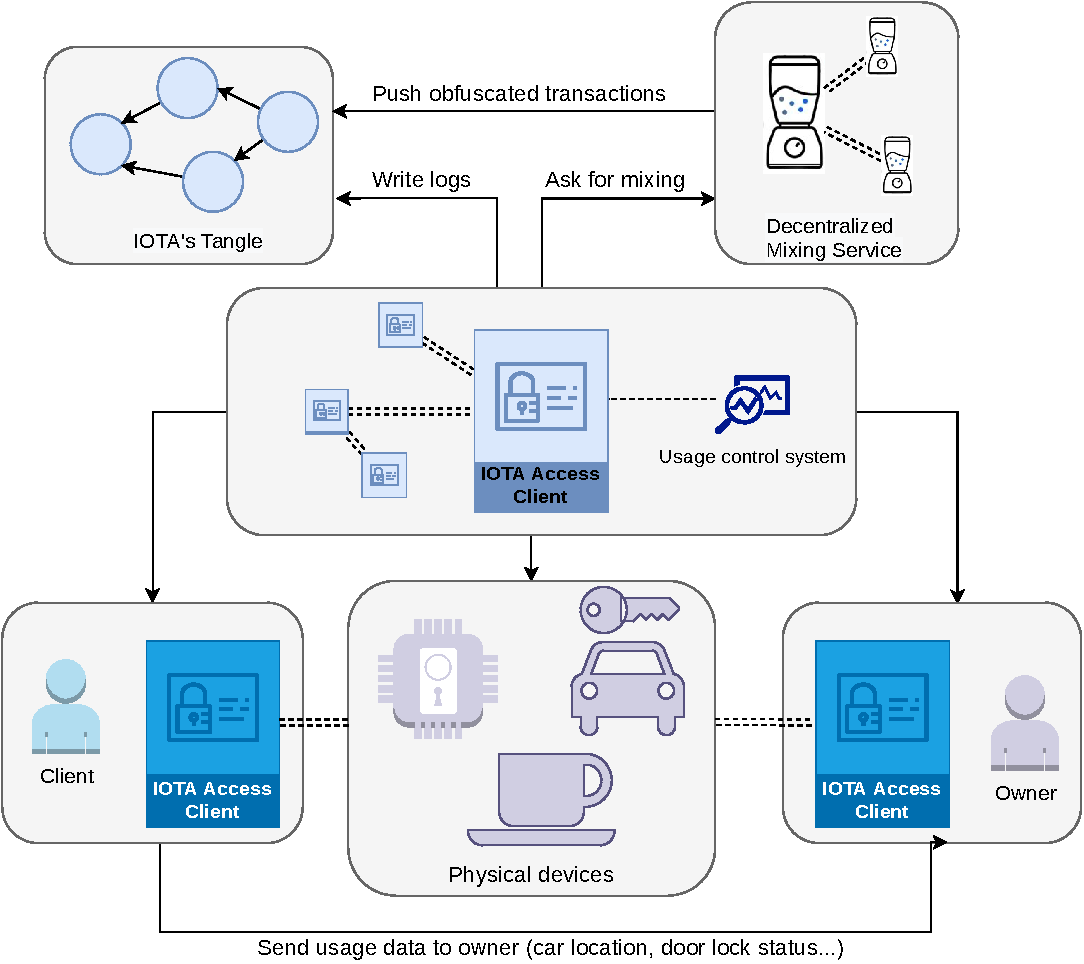
\includegraphics[width=0.75\textwidth]{Images/framework_IFIP.pdf}
    \caption{Framework to monitor data usage and physical access to IoT devices based on privacy-preserving transactions}
    \label{F_framework_IFIP}
    \end{figure*}
  
  \rul{IOTA and IOTA Access have been developed and maintained by the IOTA foundation and the mixing scheme has been proposed by Sarfraz \emph{et .al}} \cite{Sarfraz2019}.  
  IOTA and usage control have been already described in previous sections (respectively, Section \ref{S_iota_dlt} and Section \ref{S_usage_control}). In the following, 
  we detail the two other components of the framework, IOTA Access and the decentralized mixing service for IOTA.  
 \subsection{IOTA Access}
 
 IOTA Access is a lightweight access control framework tailored for resource-constrained networks.
 It is based on XAIN's FROST project, which is the byproduct of Leif-Nissen Lundbaek's Ph.D. Thesis at Imperial College London \cite{Lundbaek2020}.
 The framework is also expanded with relevant concepts, such as obligations and the delegation of access-control policies,
  to particularly address the need for reliable and secure human-machine interactions in the IoT. Notably, IOTA Access 
  introduces the concept of \emph{actions}, which are all the authorized actions that a user can perform. Actions 
  are based on \emph{attributes, obligations} and \emph{conditions}, very similar to the UCON notions with the same terminology (cf. Section \ref{S_usage_control}), but used
  in the context of physical access instead of data access. In particular, empowered by obligations and conditions, it is possible with IOTA Access to:
     1) grant or deny access at any time;
    2) charge users for physical access with zero-fee transactions; 3) set complex access restrictions based on conditions and obligations.
    To do so, IOTA Access is divided into three components, represented in Figure \ref{F_iota_access}:

    \begin{itemize}
      \item the \emph{IOTA Access client}, which is a mobile access client used as the user interface,
       both for creating policies and initiating access requests. IOTA Access contains an Android-based reference implementation;
       \item the \emph{IOTA Access server}, the embedded software executed on the device for which access will be delegated;
       \item the \emph{IOTA Access policy store}. It consists of interface servers for managing policies;
    \end{itemize}
  

 \begin{figure*}[t]
   \centering
    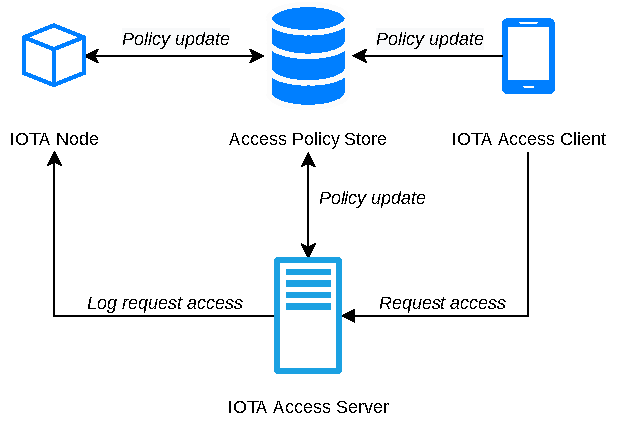
\includegraphics[width=0.6\textwidth]{Images/iota_access.pdf}
   \caption{IOTA Access framework representation}
   \label{F_iota_access}
   \end{figure*}

 The interactions between the IOTA Access components are as follows, also represented in Figure \ref{F_iota_access}. Users deploying an IOTA Access client can either request access to devices or update access policies enforced on their own devices.
 In the first case, if a user requires access to a device, the IOTA Access server evaluates the request against the policy, then logs the 
 request on the IOTA ledger, possibly using a private Tangle rather than the public ledger. In the second case, a user-triggered policy update causes a chain of network exchanges between the IOTA Access components.
First, the IOTA Access clients directly update the policies in the IOTA Access policy store, which forwards the update to the IOTA Access server and notifies the IOTA node of the update for logging purposes. 

IOTA Access is used in the proposed framework to extend the zero-fee privacy-preserving transactions to the Internet of Things devices, 
instead of restricting them to data-sharing use cases.
 \subsection{Decentralized mixing for IOTA.}
 \label{ss_decentralized_mixing_iota}
Coin mixing has been introduced in Section \ref{ss_obfuscation_coin_mixing_merge_avoidance} as one of the most common tools to obfuscate transactions 
in distributed ledgers. Coin mixing aims at removing the link between the sender and the receiver of a transaction, to complicate re-identification attacks.
However, centralized coin mixing creates significant security and privacy risks. The centralized mixing service is a likely target for denial of service 
attacks and may steal the funds or keep the transaction records for itself (cf. Section \ref{ss_obfuscation_coin_mixing_merge_avoidance}). 
However, decentralization is troublesome due to the possibility to conduct edge insertion attacks. While this is true for most public blockchains, which require transaction fees, it is 
different for IOTA due to its transaction mechanisms.

Indeed, Sarfraz \emph{et al.} \cite{Sarfraz2019} designed a decentralized mixing scheme for IOTA that leverages zero-fee transactions 
and does not require changes in the IOTA protocol. The mixing scheme has the following attractive features:
\begin{itemize}
  \item protection against signature forgery and the guarantee that
  even in the presence of malicious adversaries during mixing,
  no participant can reveal portions of his/her private key of the
  input address. This property is guaranteed by \emph{multi-signatures};
  \item fully decentralized mixing operation;
  \item no mixing fees from participant;
  \item anonymity, availability and correctness are guaranteed (cf. Section \ref{ss_obfuscation_coin_mixing_merge_avoidance});
\end{itemize}

\textbf{Mixing preliminaries.} \rul{We now introduce further considerations on IOTA addresses and mixing for a better understanding of the mixing protocol which will be detailed next. An IOTA \emph{transaction} is a transfer of IOTA tokens between a set of IOTA
addresses. To issue a transaction, a user
specifies one or more input addresses $A_{1},..., A_{n}$ with a
positive value $z$ and output (receiving) addresses $A_{1},..., A_{n}$. IOTA also supports \emph{zero value} transactions, without any input addresses. In order to
spend from an input address, a user needs to
sign the transaction with the corresponding private key to prove it owns the input address. 
}

\rul{\emph{IOTA addresses} are defined using a ternary numeral system and have a length of 81 trytes. A private key is associated with each address, whose size is determined according to a security level $s$. Once the private key is generated, it is hashed into 27 fragments that are each hashed 26 times. The hashed key fragments are used to generate an address. }

\rul{A \emph{multi-signature scheme} is a digital signature scheme that allows a group of users rather than a single one
to sign a document. A multi-signature, in cryptocurrencies, enables a group of people to formally agree on spending. Ideally, all participants need to sign the transaction from a multi-signature address, but certain variations in the
multi-signature scheme $(m, n)$ allow ownership to a given number of participants. A $(m, n)$-threshold signature scheme is a digital signature scheme where any $m$ or more signers from a group of $n$ signers can produce signatures on behalf of the whole group. In order to create a multi-signature address all participants need to share their \emph{digests} publicly, which are then concatenated to make a long single
digest. Then the same process is followed
to create a multi-signature address of 81 trytes.}

\textbf{Mixing protocol design.} We now detail the actual decentralized mixing protocol. It is composed of three different phases: \emph{settlement} (1), then \emph{output shuffling} (2) 
and finally the \emph{transaction} (3) \cite{Sarfraz2019}, all represented in Figure \ref{F_mixing_iota}. In case the protocol can not be completed, another additional \emph{fallback} phase is introduced. The protocol is detailed with $n$ peers, but to achieve anonymity, the protocol requires at least two participants. The first \emph{settlement} phase (1) \rul{using a} ($1, n$) \rul{multi-signature scheme} unfolds as follows :

\begin{enumerate}
  \item[(1a)] each peer $i \in \{1,..., n\} | k_{i},... k_{n} \in {0,1,2,... } $ determines key indexes $k_{1},..., k_{n}$
  and security levels $ s_{1},..., s_{n}$ | $s _{i},..., s_{n} \in {1, 2, 3}$. s is a security level that results in a 
  key of length $ l = s * 27 * 81$ trytes. $k_{i}$ and $s_{i}$ are used to generate digests $d_{i}$ for $i \in {1,..., n}
  $ and private keys $ pr_{1},..., pr_{n}$;
  \item[(1b)] each peer shares the digests $d_{1},..., d_{n}$ to generate $M_{1},...,M_{n}$ multi-signature addresses such that the addresses-digests mapping $M$ is
  \begin{center}
    $M = \left\{\begin{array}{l}M_1 \rightarrow D_{i(1)}, \ldots, D_{n(1)} \\ M_2 \rightarrow D_{i(2)}, \ldots, D_{n(2)} \\ \ldots \\ M_n \rightarrow D_{i(n)}, \ldots, D_{n(n)}\end{array}\right\}$
  \end{center}
  \item[(1c)] for each generated multi-signature address, every $n - i$ peers share their private keys $pr_{1}, pr_{2},..., pr_{n}$ to make a ($1,n$) 
   mapping for address ownership;
   \item[(1d)] Each peer makes a transaction $T_{i}$ to the multi-signature address $M_{i}$;
\end{enumerate}

Mixing peers validate the multi-signature address by sharing digests. If the address validation fails, then a malicious participant may be 
involved in the settlement process. The protocol aborts and all participants receive a notification. The settlement phase is followed by 
the output shuffling phase. The output shuffling phase aims to randomize the set of output addresses declared by the peers, 
preventing peers from mapping input addresses to output addresses. \emph{Shuffling} (2) unfolds as follows:

\begin{enumerate}
  \item[(2a)] each peer creates an IOTA output address $O_{1},...,O_{n}$ corresponding to input addresses $A_{1},..., A_{n}$;  
  \item[(2b)] each participant generates a key pair $(E_{i},D_{i})$ and broadcasts its public key:
  \item[(2c)] once all keys have been broadcast, the first peer creates a layered encryption of its output address, which means 
  that it encrypts its output address with all the keys of the other peers. The first peer then forwards the ciphertext to the next participant;
  \item[(2d)] each following participant $i$ up to the last one $n$ decrypts the outermost layer of encryption for all ciphertexts 
  with its corresponding decryption key $D_{i}$. Each peer receives a list of ciphertexts of size $i -1$ ;
  \item[(2e)] after decrypting the outermost layer of all the ciphertexts, each participant $i$ randomly shuffles the ciphertexts 
  and then creates a nested encryption for its output address $O_{i}$;
  \item[(2f)] the last participant decrypts all the ciphertexts and
 shuffles the final decrypted list with its output address. Finally, the final list of output addresses is forwarded to 
 the other participants.
\end{enumerate}

Upon receiving the decrypted list, the participants check if
their output addresses are actually in the list. If there is a duplication of output addresses 
or if any output address is missing from
the list, the protocol interrupts and peers enter the fallback phase. Additionally, if the decryption fails or multiple decryptions
lead to the same output, the corresponding participant aborts the
protocol and notifies every participant and all the
participants enter the fallback phase as well. If the shuffling phase unfolded correctly, the peers can enter the last transaction phase.

The purpose of the transaction phase is to build and push the final transaction to the network, i.e., the iotas from each input address $A_{1},..., A_{n}$ 
will be transferred to each corresponding output address $O_{1},...,O_{n}$. As input addresses are multi-signature, it is required 
that all the participants sign each transaction. The \emph{transaction} phase (3) is made up of the next steps:
\begin{itemize}
  \item[(3a)] every participant creates a mixing transaction that spends IOTA tokens from each
  of the input addresses in $(A_{1},...,A_{n})$ to $( O_{1},...,O_{n})$.
  \item[(3b)] the participant $i$ signs the transaction according to the specification of the IOTA protocol and broadcasts the signature $S_{i}$;
  \item[(3c)] when it receives a valid signature $S_{j}$ from another peer $j$, the peer $i$ adds all the signatures in the bundle.
 Participant $i$ checks if any other participant has spent their money saved for mixing. 
 If a participant spent its funds, the protocol is aborted and the fallback phase is triggered;
 \item[(3d)] the participant $i$ receives two transactions to approve as part of the IOTA transactional protocol (cf. Section \ref{S_iota_dlt}),
 performs the proof of work to prevent spamming, then generates the transaction hash 
 and broadcast the bundle ($S_{1},...,S_{n}$) to the IOTA network.
\end{itemize} 

If the transaction phase is completed, the mixing process is achieved and the mixing desired properties, i.e., anonymity, availability and correctness, are provided.
However, at any step of the mixing process, the protocol can enter the fallback phase in case of misbehavior. 
The protocol needs to be run again with new unused output addresses for correct protocol execution. 
The full protocol with a correct execution, i.e., excluding the fallback phase, 
is represented in Figure \ref{F_mixing_iota} \rul{with three honest participants}.

\rul{The first \emph{settlement} phase (1) unfolds as follows.  Alice, Bob and Charlie generate the multi-signature addresses $M_1, M_2$ and $M_3$ and share their corresponding private keys. The three participants then make the transactions $T_1, T_2$ and $T_3$ to the generated $M_1, M_2$ and $M_3$ addresses respectively (step 1d).
After the settlement starts the \emph{shuffling} phase (2).
In step (2a), the participants Alice, Bob and Charlie generate output addresses $O_{1}, O_{2}$ and $O_{3}$ respectively. In the next step (2b),
each participant except for Alice creates an encryption and decryption key pair. Bob and Charlie broadcast their encryption keys
$E_{k}B$ and $E{k}C$. In the following step (2c), Alice sequentially encrypts her output address $O_{1}$ i.e., Alice first encrypts for Charlie obtaining $c_1 = E(E_{k}C, O_1 )$ and then for Bob obtaining $c2 = E (E_{k}B, c_1 )$. Alice finally adds $c_2$ to a list $L = (c_2)$ and forwards $L$ to Bob. In steps (2e) and (2f), Bob receives $L$
from Alice, then decrypts the outermost layer of the cipher text $c_2$ in the list
$L$, obtaining $c_1$ . Bob also creates a new cipher text $c_3 = E ( E_{k}C, O_2)$
for his output address $O_2$ and adds it to $L$. Bob then shuffles the
list $L = (c_1, c_3 )$ and passes $L$ to Charlie. Following step (2f), Charlie
receives the list $L$ from Bob, then decrypts the outermost layer for
both cipher texts $c_1$ and $c_3$ in $L$ and obtains $O_1$ and $O_2$. Charlie adds
his address $O_3$ to the decrypted list, performs a shuffle over the
final list and broadcasts the final list.
Upon receiving the decrypted list, every participant verifies if
his or her output address is in the list. If any output address is duplicated or is missing from the list, the protocol is interrupted and the participants enter the fallback phase. Additionally, if the decryption fails or if multiple decryptions
lead to the same output, the corresponding participant aborts the
protocol, announces this anomaly to every participant and all the
participants enter the fallback phase. Otherwise, the participants can proceed to the \emph{transaction} phase (3).}

\begin{figure*}[t]
  \centering
   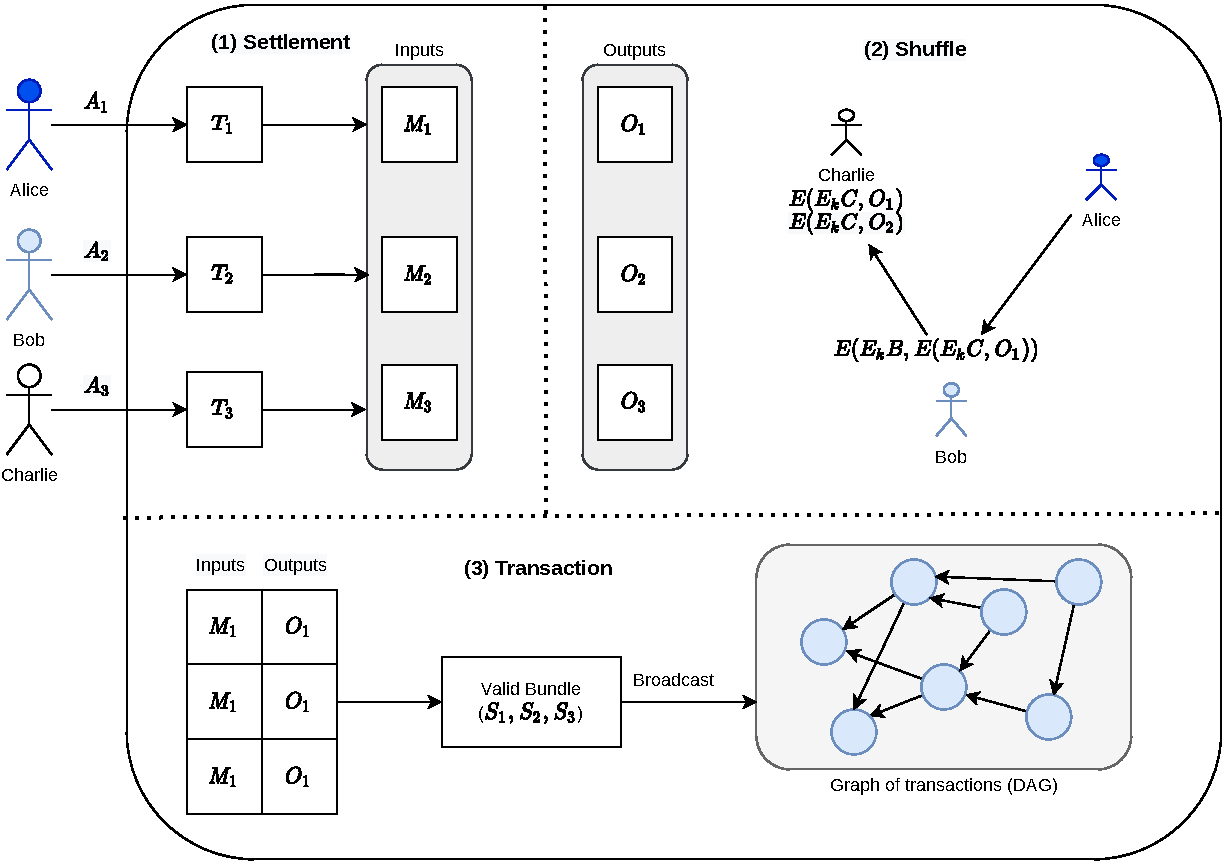
\includegraphics[width=\textwidth]{Images/mixing_iota.pdf}
  \caption{Three phases of decentralized mixing (settlement, shuffle, transaction) on the IOTA network with three peers \cite{Sarfraz2019}.}
  \label{F_mixing_iota}
  \end{figure*}
  
% \section{Performance optimization}
% \label{S_performance_optimization}

%   The proposed framework is designed to answer the performance, security and privacy needs of the Internet of Things. To ensure the system is consistent with the performance requirements, we assess the performance of the proposed framework in this section. In IOTA 2.0 \cite{Popov2020}, IOTA is decentralized and has a high throughput, low latency, high scalability and low storage overhead due to pruning.
%   However, the introduction of the UCS, IOTA Access and the mixing service likely introduces computation and network overheads, requiring further testing.
  
%   The evaluation of IOTA's network metrics, such as scalability and throughput is not addressed by this evaluation. This section aims at demonstrating the framework is viable even though it relies upon numerous technologies, and is evaluated in terms of:
%   \begin{itemize}
%       \item \emph{Quality of service}: the entire chain of events leading to access is completed in a reasonable time frame;
%       \item \emph{Computational power}: the hardware requirements are reasonable as regards Internet of Things constraints.
%   \end{itemize}
  
%   Regarding the Quality of Service, the focus is given to determining the time required for a user to be granted access after its payment. Average, minimum and maximum times will be considered. Additionally, several hardware configurations are tested, to assess whether the UCS can be deployed on resource-constrained devices.
   
%   \subsection{Configuration}
%   \label{ss_configuration}
  
%   \textbf{Configuration of the IOTA node.}
%   To reduce computation and network overheads introduced by the usage control system, several optimizations are set up: the usage control system deploys an IOTA node to integrate the IOTA network. This integration provides several benefits. The UCS can prioritize its transactions and perform local analysis on its ledger without querying the other IOTA nodes. Secondly, the IOTA node is configured, by removing the possibility to compute proofs of work for other users and by using \emph{spammers} to speed up the network by validating tips (cf. Section \ref{S_iota_dlt}), in particular when the network is in a low load regime.
%    Spammers are useful for testing as well, as the results are different whether the tests are conducted in a low load or high load regime.
%   The principles of integration, as well as its benefits, are fully detailed in the dedicated Section \ref{S_integration_usage_control_with_dlt}. 
%   As IOTA transaction throughput increases with the number of users, i.e. when many users push new transactions, it is relevant to use spammers that create zero-value transactions\footnote{zero-value transaction do not transfer iotas and the transaction corresponding amount is zero, hence their name} and validate two pending transactions from other users in the process. Spammers are implemented to ensure transactions do not take too long to be validated during low load regime.
%   Small devices with very poor computation capacities or with energy constraints can delegate their proof of work to a node. Our node is configured to refuse delegations to focus on usage control.
  
%   \textbf{Methodology and network configurations.}
%     We measure the time needed for a transaction to be validated and pushed to the network, and the time to fetch the transaction from an IOTA node. These operations correspond respectively to the calls \texttt{buildTransaction}, \texttt{push} and \texttt{checkTransaction} in the sequence diagram of Figure \ref{F_sequence_ifip}. 
%     Tests are conducted in three different configurations: (1) the IOTA remote node which is a resource-constrained node, to help understand the behavior of the solution in a fully constrained IoT environment, (2) the IOTA remote node which is no longer resource constrained to measure the gain from lifting the resource limitation, and (3) a local node which supports both the UCS and IOTA node, as illustrated in Figure \ref{F_framework_integration}.
%     For each test, one thousand samples ($N=1000$) are used. The resulting experimental measurements are summarized in Table~\ref{tab:metric}.

%     \textbf{Note on reproducibility.} The tests provided in this section are performed on the IOTA public test network. This is troublesome 
%     for reproducibility reasons (cf. Section \ref{ss_testbed}), but these tests have the following benefits:
%     \begin{itemize}
%       \item it is a first evaluation on a large-scale network to show that integration is a relevant process for performance. \cul{Addressing the challenges of large-scale networks is one of the purposes of this thesis work, justifying an evaluation on an appropriate network} (cf. Section \ref{S_assumptions}) ;
%       \item it enables estimating the outcomes of integration on a public network with a subsequent high number of nodes, rather than on a test network
%       with fewer nodes.
%     \end{itemize}

%     As a consequence, these tests are still considered in this chapter, not to demonstrate the validity of integration, but 
%     for informative purposes. Testing to demonstrate the validity of the integration process is provided in 
%     the dedicated section (Section \ref{S_performance_evaluation}) of Chapter \ref{C_integration}. 
%  \begin{figure*}[t]
%   \centering
%    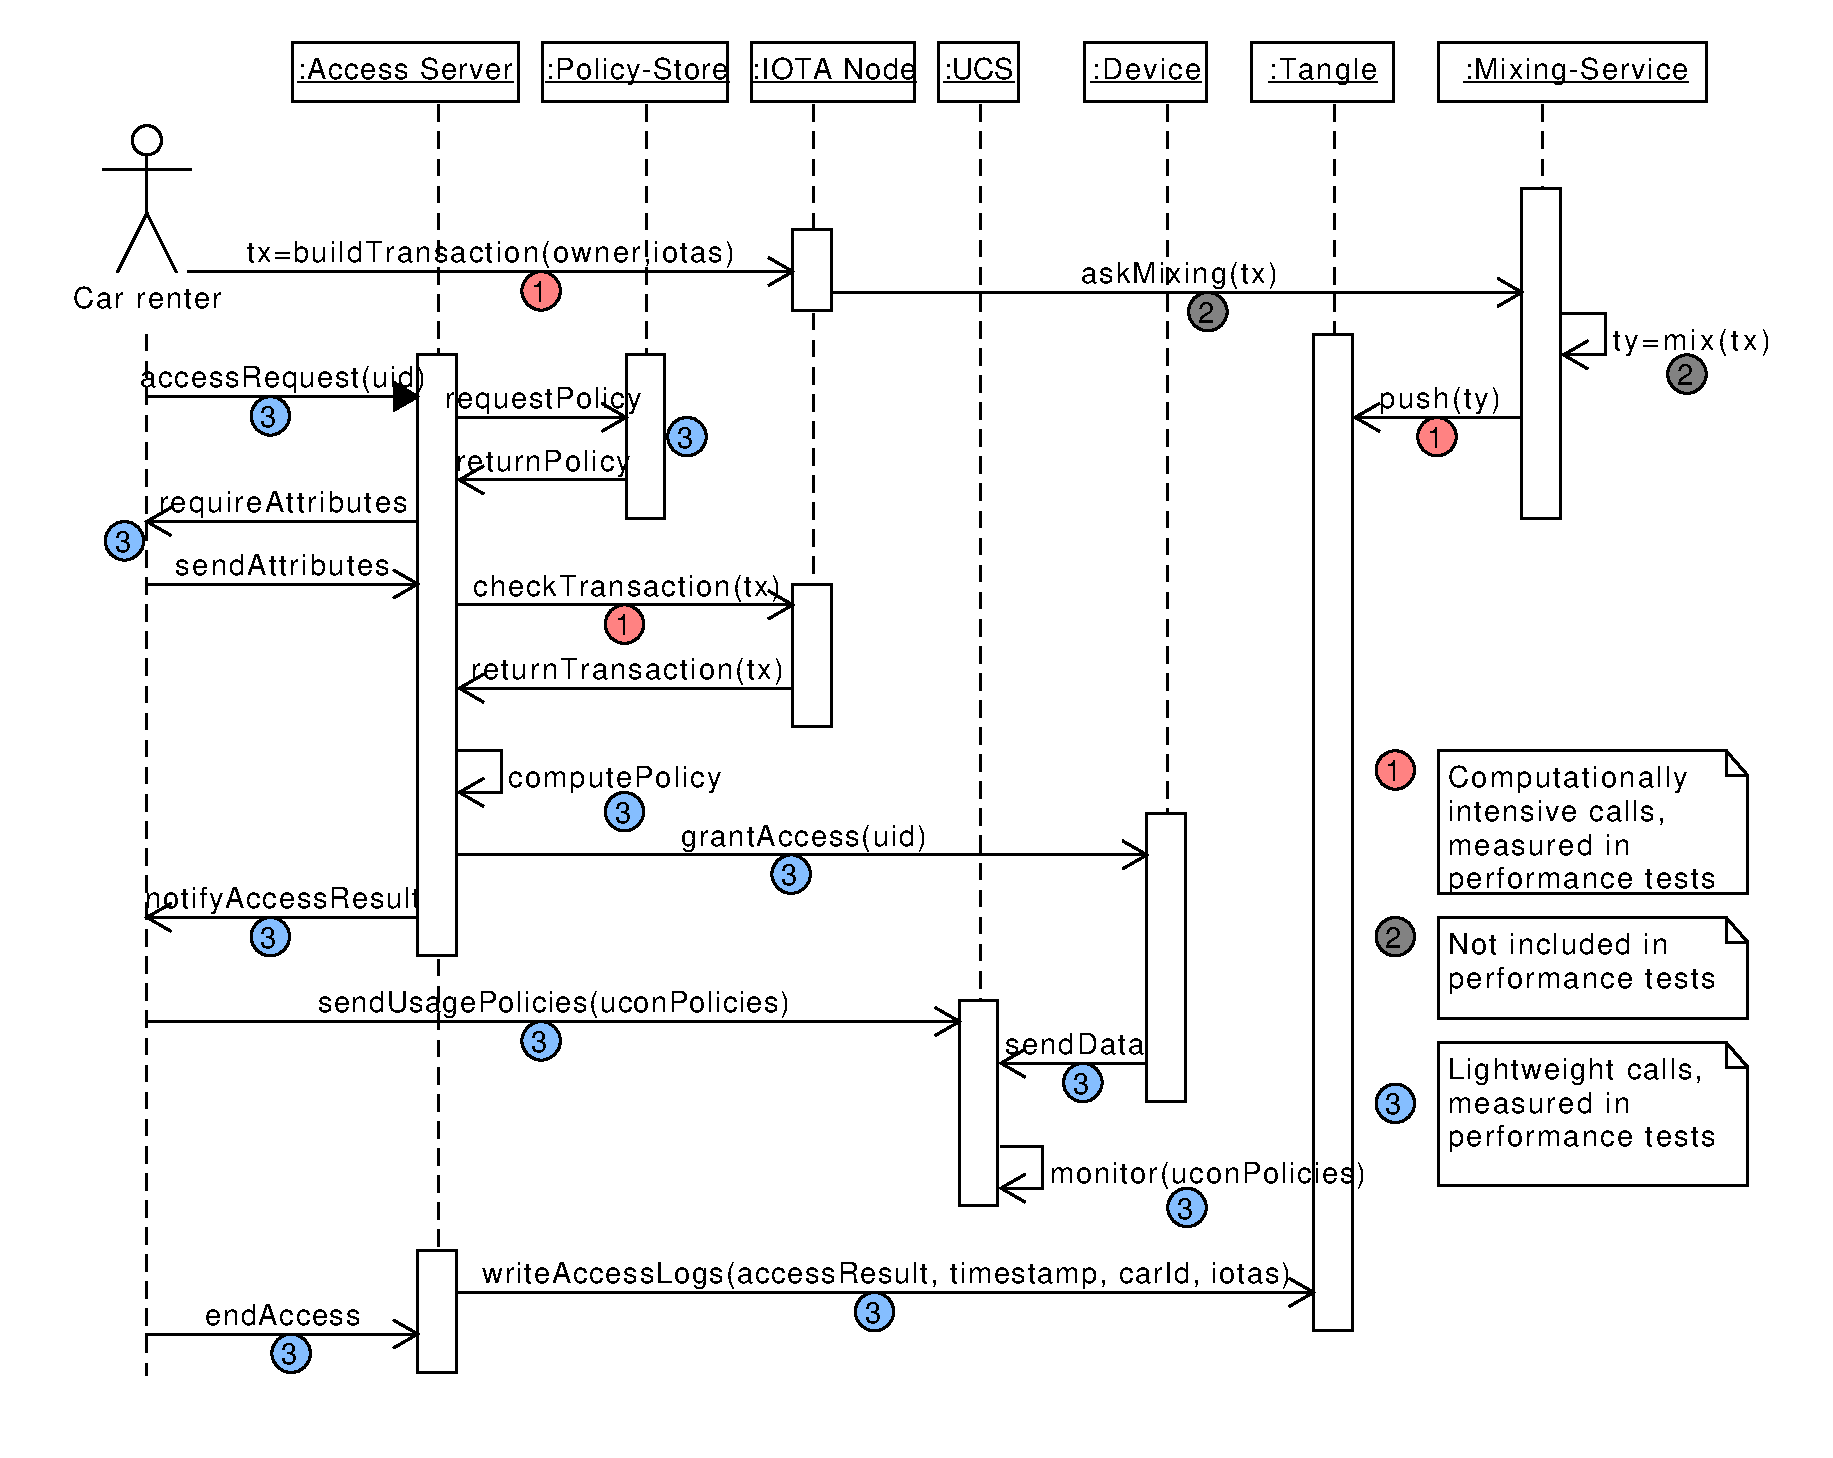
\includegraphics[width=\textwidth]{Images/sequence_ifip.pdf}
%   \caption{Workflow of a data access request using IOTA, IOTA Access and the mixing service.}
%   \label{F_sequence_ifip}
%   \end{figure*}

% \subsection{Evaluation results.}
%   \textbf{Resource-constrained remote testing.}
%     To demonstrate the possibility of a usage control system interacting with IOTA on resource-constrained devices, the performance tests are first conducted on a virtual machine with 4096MB of RAM and an Intel Core i5-10210U CPU @ 1.60GHz (1 core). The number of transactions per second \emph{on the test network} was oscillating between 3 TPS and 11 TPS on the test network, up to 16 with the spammer. The delegated proof of work is removed as part of the optimizations.
%     Pushing a transaction on a remote resource-constrained node (RCN) takes on average $\overline{t}_{push,rcn}= 5271ms$. Additionally, the usage control system takes an average $\overline{t}_{fetch,rcn}=45ms$ to fetch the transaction result from the remote node, accounting for a total $\overline{t}_{rcn}=5316ms$ on average as arithmetic mean is linear.
%     The time needed to create and push a transaction can tremendously vary, from a minimum $m_{rcn}=364ms$ to a maximum $M_{rcn}=26851ms$, which is reflected by a standard deviation of $\sigma_{rcn}=4629ms$. This difference is mostly due to the synchronization between peer nodes, which increases the transaction time significantly when the node is lagging or one of the peers disconnects. The confidence interval is $I_{rcn}=\overline{t}_{rcn}\pm1.96\frac{\sigma_{rcn}}{\sqrt{N}}=5316\pm287ms$.

%     The results show that the solution can be deployed on a machine with low computation capacities. However, with delays of up to 26 seconds to create, validate and push a transaction to the network, this can be unsatisfying in some use cases, e.g.  accessing a vehicle or 
%     opening a door lock.

% \textbf{Resource-unconstrained remote testing.}
% The IOTA remote node is now run on a computer with more computing power, with an Intel Core i5-10210U CPU @ 1.60GHz (4 cores) and 8192MB of RAM supporting the optimizations. This corresponds to the high-end Raspberry Pi 4 Model B specifications\footnote{https://www.raspberrypi.com/products/raspberry-pi-4-model-b/specifications/}.

% Pushing a transaction on a remote node (RN) with more computing capacity takes on average $\overline{t}_{push,rn}= 1867ms$. Additionally, the usage control system takes on average $\overline{t}_{fetch,rn}=45ms$ to fetch the transaction result from the remote node, accounting for a total $\overline{t}_{rn}=1912ms$ on average.
% The time needed to create and push a transaction is still very variable but spreads out less, from a minimum of $m_{rn}=363ms$ to a maximum of $M_{rn}=12209ms$, with a standard deviation of $\sigma_{rn}=1499ms$. The samples express a significant impact of the UCS computation power when creating and pushing transactions to a node. The confidence interval is $I_{rn}=\overline{t}_{rn}\pm1.96\frac{\sigma_{rn}}{\sqrt{N}}=1912\pm93ms$.

% The tests are also conducted using a much more powerful device, with 32GB RAM Memory and an Intel Core i5-1021UCPU @ 1.60GHz (8 cores). The purpose is to see if there is a limit in speed improvement as the UCS computation power increases. The results are very similar to the 8GB RAM setup, in the same confidence interval. 

% \textbf{Local testing.}
% The IOTA node is deployed on the local node (LN) running the UCS, as illustrated in Figure \ref{F_framework_integration}. The network connection, expressing the capacity of the local node to quickly get updates from other nodes, provides 98 Mbps in downlink and 77 Mbps in uplink. The node and the UCS run on the same device with 8192MB of RAM Memory and with the Intel Core i5-10210U CPU @ 1.60GHz (4 cores).
% The optimizations are also enabled. 
% The average time for a node to validate a transaction drops from $\overline{t}_{rn}=1912ms$ to an average $\overline{t}_{ln}=1579ms$. The minimum transaction time on a local node dropped from $m_{rn}=363ms$ to $m_{ln}=10ms$, while the maximum changed from $M_{rn}=12209$ to $M_{ln}=9830s$. The standard deviation is $\sigma_{ln}=1544ms$. The confidence interval is $I_{ln}=\overline{t}_{ln}\pm1.96\frac{\sigma_{ln}}{\sqrt{N}}=1579\pm96ms$.

% \begin{figure*}[t] 
%   \centering
%    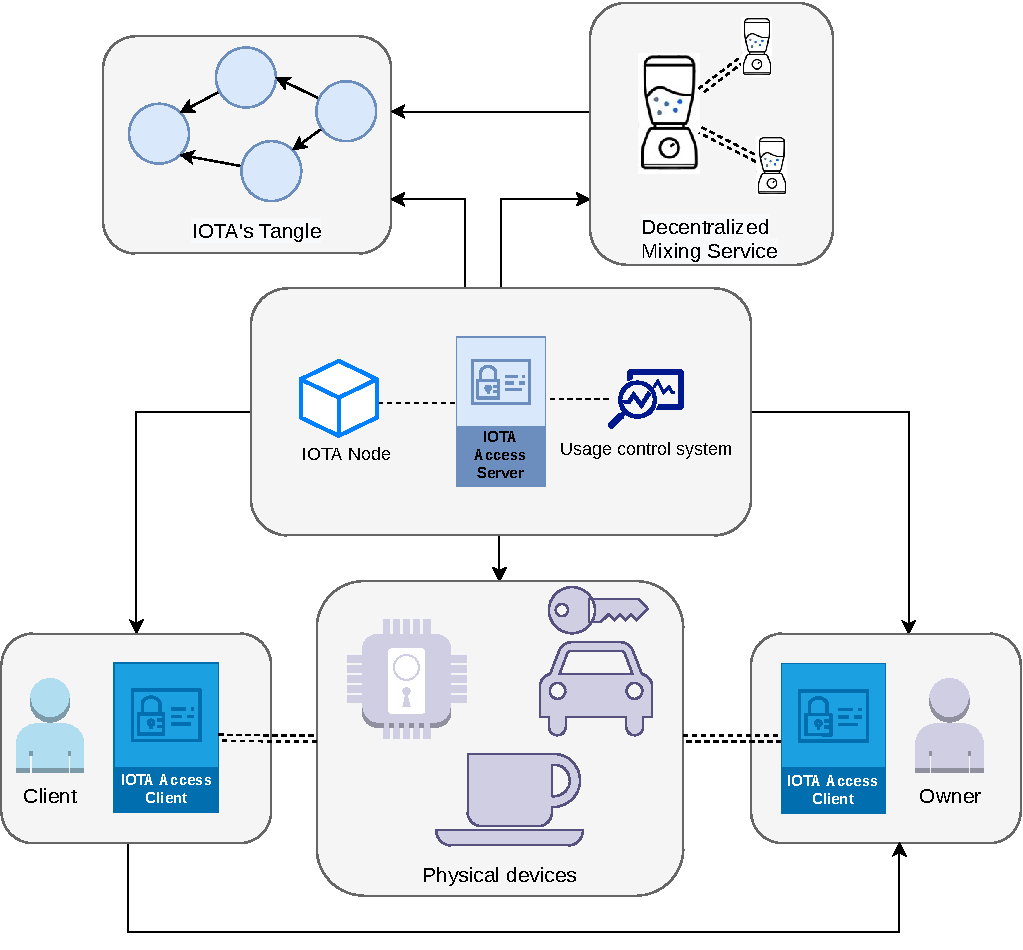
\includegraphics[width=0.68\textwidth]{Images/framework_IFIP_integration.pdf}
%   \caption{IOTA node deployment for optimization}
%   \label{F_framework_integration}
%   \end{figure*}
% % \subsubsection{Optimised local testing.}
% % The performance tests have been performed again with a local and optimised node (LO), on the same device as the UCS: first, the use of a spammer pushing four zero-value transactions per second. Secondly, the removal of delegated Proof of Work by our node. The average time for a node to validate a transaction further dropped from $\overline{t}_{ln}=1579ms$ to an average $\overline{t}_{lo}=XXXms$ on the local node. The minimum remained the same, $m_{lo}=10ms$ while the maximum further dropped from $M_{rn}=9830$ to $M_{lo}=XXXs$. The standard deviation is $\sigma_{lo}=XXXms$. The confidence interval is $I_{lo}=\overline{t}_{lo}\pm1.96\frac{\sigma_{lo}}{\sqrt{N}}=XXX\p

% As a result, using a local node has the following outcome:

% \begin{enumerate}
%     \item a 17.5\% decrease on the average transaction time;
%     \item transactions can be processed very quickly, taking a minimum of 10ms instead of a minimum $363ms$;
%     \item the maximum time only drops from $12209ms$ to $9830ms$, which remains convenient for real-life applications;
%     \item almost half (48\%) of the transactions are processed within a second, compared to 34.5\% for transactions using a remote node.
% \end{enumerate}

% \textbf{Additional calls.}
% While the performance tests are conducted on the three computationally intensive calls, the other category called \emph{lightweight calls} (cf. Figure \ref{F_sequence_ifip}) has also been measured. 
% The calls \texttt{accessRequest}, \texttt{requestPolicy}, \texttt{requireAttributes}, their corresponding return values \texttt{notifyAccessResult}, \texttt{sendAttributes}, \texttt{returnPolicy}
%  as well as \texttt{grantAccess} and \texttt{endAccess} consist in messages exchanged between the actors. They are strongly correlated to the time needed to communicate between the car renters, the access server, and the policy store. 
%  These calls took under 1ms to be achieved in our setup since they were all running locally on the same device. 
%  These three entities can be considered as close (in space) and the time for all these calls is negligible compared to the \texttt{buildTransaction}, \texttt{push} and \texttt{checkTransaction} calls.

% The remaining calls have different behavior. \texttt{computePolicy} is composed of several boolean operations, taking a negligible time. \texttt{sendUsagePolicies} and \texttt{sendGPSData} are operations
% that are continuously repeated until the access is terminated using the \texttt{endAccess} call or if \texttt{monitor} detects a violation of the policy. The time needed to \texttt{monitor} the access according to a given policy was measured and takes an average $\overline{p}=5ms$ for a simple policy made of three rules. 
% Finally, the call \texttt{writeAccessLogs} is very similar to \texttt{buildTransaction} as a message on IOTA is built as a zero-value transaction. However, it does not require checking balances and the construction of the transaction is simpler. A log takes an average $\overline{l}_{lo}=473ms$ to be built and pushed to 
% the network, on a local node using 1000 samples. Besides, the call \texttt{writeAccessLogs} does not impact the Quality of Service of the users as it is
% performed after the access is terminated.

% In conclusion, the experiments have shown that the framework fulfills the performance requirements, regarding the quality of service and the computational power (cf. Section \ref{S_performance_optimization}).  
% The time needed to validate the access to a user requiring it is acceptable, and resource-constrained devices can run a usage control system and interact with an IOTA node. 
% The IOTA node itself can run on a machine corresponding to Raspberry Pi Model B, as we did in the local testing section.  

%     \begin{table}[h]
%       \resizebox{\textwidth}{!}{%
%         \begin{tabular}{|c|c|c|c|c|}
%           \hline
%           \textbf{Test category} & \textbf{Min} & \textbf{Max} & \textbf{Average} & \textbf{Standard deviation $\sigma$} \\
%           \hline
%           Remote (constrained) & 364ms & 26851ms & 5316ms & 4629ms \\
%           Remote (unconstrained) & 363ms & 12209ms & 1912ms & 1499ms \\
%           Local & 10ms & 9830ms & 1579ms & 1544ms \\
%           \hline
%         \end{tabular}}
%         \caption{Performance measurements for different test configurations}
%         \label{tab:metric}
%       \end{table}    

\section{Security and privacy evaluation}
\label{S_security_and_privacy_evaluation}

As part of the research \hyperref[obj:56]{\emph{Objective 5}} (cf. Section \ref{S_problem_statement})
, this section analyzes the privacy and security risks in the system. To better identify the privacy and security threats and how they are mitigated by the proposed framework, we first introduce a car sharing illustrative scenario.

\subsection{Car sharing system illustrative scenario}
\label{ss_illustrative_scenario}


\emph{Car sharing} is a model of car rental where people rent cars for a short period. They differ from classic rental models in that the owners of the cars are individuals instead of an agency.
The context is dynamic as many users may enter or exit the car club during the day. For the users to interact with the system, a mobile application is used for registration and requiring access to the cars.

For security purposes, car owners have the right to monitor their cars and collect their real-time location. However, the location of the car also produces data about the car renters which are sent to the car owners. Car owners use a mobile phone application to define the access policy for their cars. Similarly, car renters define usage control policies using the same application. Car renters use public distributed ledger technology to make decentralized and transparent transactions. Car renters as well as car owners have one or several addresses on the IOTA network, to either send or receive transactions.


\subsection{System agents} The agents of the car renting system can be summarized as follows:

\begin{itemize}
    \item the car owners put their vehicles on the renting market;
    \item the car renters pay for renting the vehicles;
    \item the cars themselves send data to the owners such as location, and whose access is monitored;
    \item the Access Server (AS) is responsible for managing the access to the cars;
    \item the Usage Control System (UCS) monitors the data generated by other agents;
    \item the mixing server obfuscates the transactions to preserve privacy.
\end{itemize}

 Both the Access Server and the Usage Control System control access, respectively to a physical object - the car - and to the data. The UCS also monitors the information flow, blocking data dissemination to forbidden actors.

%  \rul{The next security and privacy threat analyses, in the context of the scenario, focus on the threats associated with the geolocation data of the car renter. As a consequence, the security analysis focuses on the usage control system as the main security component accountable for the privacy of the car renter. Note that apart from geolocation data, other kinds of data are privacy-sensitive and can be used to carry out inference attacks, such as the habits of car renters and car owners. Besides, the threat analysis could have been centered on car owners or on the decentralized mixing service, which are also privacy-sensitive. Yet, the choice to focus on car renters is motivated by the fact that the mitigations put in place can be extended to other privacy-sensitive data. Therefore, enumerating all possible threats in the system does not help to demonstrate the relevance of the framework and is a complex process.}
\subsection{Security and privacy threat model}
\label{ss_priv_threats}

\textbf{Privacy threat model.}
Depending on the data the attackers are obtaining, and using the LINDDUN threat evaluation framework \cite{Wuyts2015} (cf. Section \ref{ss_privacy_threat_modeling}), we discuss the threat analysis for our proposed scenario hereafter. 
\begin{itemize}
    \item \emph{linkability}(L): an attacker can link the car renter and the car owner, respectively the sender and the receiver of a transaction, thus simplifying re-identification and inference; 
    \item \emph{identification}(I): the attacker can link 
    the pseudonym to the real identity of the car renters or the car owners, breaking anonymity;
    \item \emph{Non-repudiation and repudiation}(N): With repudiation, an attacker can exfiltrate information and deny it did. Note that this threat is actually \emph{a security goal} in our system, contrary to other threats. Conversely, non-repudiation can be a threat to legitimate users if an attacker can prove that a user has done some sensitive actions e.g., an illicit transaction~\cite{Wuyts2015}. In our scenario, non-repudiation is not considered a threat, but repudiation is;
    \item \emph{disclosure of information}(D): an attacker can access data about a user without having the proper access rights. Inference attacks can be included in this category and are defined as "attacks where the attacker has used existing knowledge to aid the attack”~\cite{Henriksen2016}. An inference attack occurs when an attacker can infer information from apparently harmless information. For example, in our scenario, an attacker could infer working hours by gathering transactions timestamps;
    \item \emph{unawareness}(U): unawareness occurs if car renters are not aware of the collection, processing, sharing and storage of their geolocation data;
\end{itemize}

Detectability(D) is not considered a threat as data is publicly registered on the ledger. Both the existence and the content of the data are already known to the attackers. Rather than preventing detectability, the focus is given to preventing its most important aftermath, inference attacks~\cite{Wuyts2015}.
Non-compliance(N) is considered an orthogonal issue since the regulations are country-dependent. However, distributed ledgers may have several compliance issues, such as their immutability which contravenes articles 16, 17 and 18 of the GDPR about the right to data deletion and modification~\cite{EUdataregulations2018}. Finding technical solutions to compliance issues is an active field of research~\cite{Haque2021}.

\textbf{Security threat model}
\label{ss_sec_threats}
Considering the agents defined in the car renting system, the threat model distinguishes \emph{four attacker types}:
\begin{enumerate}
    \item the single car owner, who has legitimate access to some sensitive data of the car renters;
    \item several car owners colluding to gather bigger sets of data;
    \item the mixing server that may secretly keep the links between car renters and car owners that it is supposed to remove. It can use this information to carry out re-identification attacks; 
    \item external attackers who wish to disable the UCS to help car owners disseminate data to other agents.
\end{enumerate}

The car owners are considered \emph{honest-but-curious}. They will respect the system rules by granting access to their cars upon receiving payments but will snoop on the data of the users requesting their services. Honest-but-curious attackers are assumed to rely on transactional content only to re-identify users, rather than network-level information, e.g. IP addresses. External attackers are conversely \emph{malicious} and actively try to neutralize the UCS to enable car owners to disseminate their data.

Concurrently, there are \emph{security risks} because a single agent of the system - namely the UCS - is responsible for data protection. The UCS itself is considered as \emph{trusted}. External attackers can however be interested in neutralizing the UCS to enable the collusion of car owners. Similarly to the privacy threat analysis using LINDDUN, we use the STRIDE security threat modeling \cite{Howard2006} to identify the security threats for the usage control system:
\begin{itemize}
    \item \emph{Spoofing}(S): an external attacker could masquerade as a legitimate user to be granted access to unauthorized data, or as the control system to collect the car renters' data;
    \item \emph{Tampering}(T): an external attacker could modify either the data or the infrastructure of the usage control system. Besides, an attacker could try to modify the binaries of the usage control system to make it ineffective~\cite{Kelbert2018};
    \item \emph{Denial of service}(D): the external attacker can temporarily disable the UCS, threatening the availability of the system and disabling the usage control mechanisms.
\end{itemize}

The Repudiation(R) and Information disclosure(I) risks are already tackled by the LINDDUN privacy threat model and are excluded from the security threat modeling. Finally, an external attacker can conduct an Elevation of privilege(E) by leveraging vulnerabilities as illustrated in~\cite{Babil2013} to bypass the UCS restrictions. These attacks are very diverse and implementation-dependent, therefore considered out of the scope of this thesis work.

\subsection{Privacy threats and mitigations.}
\label{ss_privacy_threats_and_mitigations} 

 Table~\ref{l_table1} describes for inference attacks each possible combination of attackers, the data types they have access to, where data is stored and an instance of a privacy leakage associated with this risk. Table~\ref{l_table2} describes other privacy threats and how they are mitigated.\rul{The focus is put on car renters as an example but the mitigations introduced can be applied to other privacy-sensitive data if: 1) the data dissemination is a privacy risk; 2) the data processing creates inference risks. Such data also include but are not limited to the car renter's driving habits or the car owner's renting habits.}

\begin{table}[h]
  \resizebox{\textwidth}{!}{%
    \begin{tabular}{|c|c|c|c|}
      \hline
      \textbf{Attacker type} & \textbf{Data type} & \textbf{Data storage} & \textbf{Example} \\
      \hline
      Honest-but-curious & Transaction & Tangle & Purpose of payment \\
      Car owner (alone) & Location & Owner's device & Renter's job \\
      Car owners (colluding) & Location & Owners' devices & Renter's job \\
      Ext. attacker \& car owners & Location & Owners' devices & Data sets on renters \\
    % Mixing service & Pseudonym &  Mixer memory & Linkage, identification & Identities of users\\ 
      \hline 
    \end{tabular}}
    \caption{Inference attacks according to the attackers' profile}
    \label{l_table1}
  \end{table}
  
Any user has access to the Tangle's transactions, which are public and contain privacy-sensitive timestamps, users' addresses and values, i.e. how many iotas are sent to a car owner. Any honest-but-curious attacker can attempt to use the blockchain transactions for inference attacks, e.g. use the number of tokens in the transactions to infer the purpose of the payment. The merge avoidance mechanism integrated into our framework reduces the risk of inference by splitting the transactions into several smaller ones, thus making it harder to guess the purpose of the transactions (cf. Section \ref{ss_obfuscation_coin_mixing_merge_avoidance}). \rul{For instance, it is harder to infer the benefits of the car owners as long as sub-addresses are not linked with one another, or to identify the purpose of the car renters transactions.}

Additionally, car owners may infer privacy-sensitive data from the car renters' location data. The location of the car renters may reveal their driving habits, their jobs, their religion or their hobbies.
Besides, colluding car owners can merge their data about a given user to increase the inference's quality or increase the number of users in their databases to improve their value.
If an external attacker successfully neutralizes the UCS, as reported in Section~\ref{ss_security_threats_and_mitigation}, car owners can freely share users' data and disseminate them to a shared database for processing. 

\begin{table}[h]
  \resizebox{\textwidth}{!}{%
    \begin{tabular}{|c|c|c|c|}
      \hline
      \textbf{Attacker type} & \textbf{Data type} & \textbf{Threat} & \textbf{Mitigation} \\
      \hline
      Honest-but-curious & Transaction & Linkability & Mixing \\
      Honest-but-curious & Transaction & Identification & No address reuse \\
      Curious Mixer & Addresses & Linkability & Mixer decentralization \\
      External attacker & Geolocation data & Disclosure & Usage and Data Flow Control \\
      Car owner & Renters' data & Repudiation & Data flow control, auditability \\
      Honest-but-curious & Renters' data & Unawareness & Usage control \\
      \hline
    \end{tabular}}
    \caption{Threats to privacy and their mitigation}
    \label{l_table2}
  \end{table}
Table \ref{l_table2} summarizes the privacy threats for the car renters excluding inference attacks, here above presented. By observing transactions, an honest-but-curious attacker may try to link the sender and the receiver. This risk is mitigated by the mixing server. Furthermore, when car renters use the same address multiple times for outward transactions, they are exposed to re-identification (cf.~section~\ref{ss_de_anonymisation}). We generate a new address in our framework for each outward transaction and forbid address reuse to mitigate this risk. Moreover, as the mixing service is decentralized (cf. Section \ref{ss_decentralized_mixing_iota}), a node involved in the mixing process can not make links between any input or output addresses. The information disclosure is prevented by the usage control system, as it monitors access to the data and prevents dissemination to unauthorized users. The repudiation threat is provided as the car owners are continuously monitored by the UCS. Finally, usage control provides a solution to unawareness as car renters have to explicitly specify how they want their data to be used. 

\subsection{Security threats and mitigation}
\label{ss_security_threats_and_mitigation}
The UCS is a critical agent for controlling data usage and data flows between the system agents. It is an attractive target, vulnerable to specific attacks which can be partially mitigated. The proposed countermeasures to the security threats established using the STRIDE model (cf. section \ref{ss_sec_threats}) are:
\begin{itemize}
    \item \emph{Spoofing}(S): legitimate users and the usage control system mutually authenticate, e.g., using SSH or TLS;
    \item \emph{Tampering}(T): the data processing is monitored by the UCS, excluding illegal modifications to the data. However, an attacker can modify the usage control system's binaries to make it ineffective~\cite{Kelbert2018}. This threat can be mitigated by digital signatures~\cite{Kelbert2018};
    \item \emph{Denial of service}(D): the modern denial of service attacks can be hard to mitigate, but decentralizing the UCS alleviates the risk, as well as mutual authentication of all the infrastructure components using certificates~\cite{Kelbert2018};
\end{itemize}

\rul{In addition to the security threats addressed by STRIDE, we complement the analysis with another critical physical security issue, which is the possibility to damage the car.}
 Car renters may damage the car and it is relevant to design a compensatory measure to make sure the car owners do not take disproportionate risks by getting involved in the network. Indeed, the framework provides a fair level of privacy and car renters are encouraged to run away without paying compensation for damaging the car. This is a strong deterrent to the car owners' involvement in the system.
As a solution, we introduce a stake that has to be locked by the car renter during a given amount of time in the form of a UCON pre-obligation. This principle is very similar to the proof of stake but is used to make access decisions rather than to achieve consensus. In proof of stake, smart contracts are needed to automatize both the rewards and the penalties, respectively for right or wrong behaviors. In our stake guarantee system, smart contracts are used to withdraw the deposit or conversely to give it back to the car renters once the access and the arbitration time are over. However, smart contracts are not yet fully implemented in IOTA, and can only be used in the test network~\cite{SC2021}. An alternative is to send the deposit to an address belonging to the usage control system as long as smart contracts are not available. Although less satisfying, this is a convenient workaround under the trusted UCS assumption.

\section{Conclusion}
\label{S_conclusion_ifip}

In this chapter, we detailed and evaluated a framework to address the requirements of privacy, security and
performance of the Internet of Things, while providing a basis for zero-fee micro-transactions (\hyperref[obj:1]{\emph{Objective 1}}). 
The basis of the framework is the IOTA DAG-based distributed ledger.
IOTA is complemented by privacy-preserving mechanisms: merge avoidance
and decentralized mixing. Finally, we added usage control so that users can monitor the usage of their data, 
and data providers sell the data generated by their devices according to pre-defined policies, including rules on transactions.

\cul{We conducted security and privacy evaluations as part of the \hyperref[obj:56]{\emph{Objective 5}} (cf. Section} \ref{S_problem_statement}) \cul{to highlight the security and privacy guarantees provided by the framework}.
The next chapter \ref{C_integration} introduces an integration method to further improve performance aspects. 
We analyze the necessary conditions to ensure integration is relevant, provide a methodology to integrate usage control 
before evaluating the outcome of the proposed integration.
 

%-------------------------------------------------------------------------------
\newpage \ \newpage
\chapter{Integration of Usage Control with Distributed Ledger Technologies}
\label{C_integration}
\minitoc

As detailed in the problem statement \ref{S_problem_statement}, one of the motivations of this thesis is to identify the methods to integrate usage control correctly in distributed ledgers, notably for performance issues (\hyperref[obj:23]{\emph{Objective 3}}). Indeed, adding the usage control system, or any privacy-enhancing technologies, to an existing distributed ledger creates additional bottlenecks. Firstly, the usage control system itself has performance limitations that sometimes exceed the ledger constraints. Besides, the interactions between the usage control system and the distributed ledger can create network or storage bottlenecks. Finally, the large number of devices in the Internet of Things creates significant network interactions between devices and the usage control system e.g., between the Policy Enforcement Points and the Policy Decision Point. This chapter focuses on the integration process. First, the existing integration schemes in the literature are introduced (Section \ref{S_state_of_the_art_ucon_dlt}). Then, we focus on identifying the most suitable technologies to integrate, as well as the purpose and methods of integration (Section \ref{S_integration_usage_control_with_dlt}). The integration process is evaluated to measure its performance benefits accurately (Section \ref{S_performance_evaluation}). A privacy threat assessment is also conducted in the general context of data trading, highlighting the benefits of usage control to preserve privacy (Section \ref{S_privacy_evaluation}), before concluding (Section \ref{S_conclusion_integration}).

\section{State-of-the-art usage control with distributed ledgers}
\label{S_state_of_the_art_ucon_dlt}

Integration of usage control with distributed ledgers, often referred to as \emph{incorporation}, has been proposed in the literature to benefit from distributed ledger properties. In particular, private blockchains are often leveraged for the following reasons:
\begin{itemize}
    \item \emph{auditability} and the possibility to monitor data while controlling data access simultaneously \cite{Khan2020, Ma2020};
    \item \emph{smart contracts} to enforce usage control and process data automatically \cite{Ma2020, Zhang2022}; 
    \item \emph{performance} with better network response time and low computation requirements \cite{Salimitari2020} in comparison with public blockchains.
\end{itemize}

Khan \emph{et al.}~\cite{Khan2020} incorporated the components of the UCON framework into the Hyperledger Composer, to form the BlockU model. The main reason stated by the authors is the continuous monitoring of the data access, thanks to attribute mutability. UCON is incorporated by using the Hyperledger Composer layer, a layer dedicated to modeling applications. Therefore, this incorporation can be seen as peripheral as the UCON components do not contribute to the blockchain network, and performance aspects are ignored. Besides, this work is not focused on IoT use cases.

Ma \emph{et al.}~\cite{Ma2020} proposed a decentralized usage control on both a public and a permissioned blockchain, respectively Ethereum and Hyperledger. A clear focus is given to privacy and decentralization to prevent accidental or intentional data leaks. All data operations are processed directly on the private blockchain with smart contracts, the degree of integration is consequently quite high. The public blockchain is used to introduce a reward mechanism, to encourage users to provide quality usage control data. However, the integration of usage control into the blockchain benefits usage control but not the blockchain network.

Shi \emph{et al.}~\cite{Shi2021} designed a Distributed Usage Control Enforcement (DUCE) solution for the Internet of Things, to tackle privacy issues related to the Cloud-Enabled Internet of Things (CEIoT). DUCE uses distributed PDP and PEP components and leverages private blockchains to store tamper-proof and traceable data on the ledger. The policies are written in the XACML language and then converted by an algorithm into the Solidity language for smart contracts. DUCE relies on a \emph{Trusted Environment Execution} (TEE) to enforce trustworthy processing of the rules.

Zhang \emph{et al.} \cite{Zhang2022} devised an efficient data trading scheme with usage control for Industrial IoT (IIoT). The scheme is based on Hyperledger Fabric and uses Intel SGX to define protected private regions of memory. Similarly to the above-mentioned related works, the authors utilize smart contracts to automatically trade data. To tackle usage control overhead on the data trading system, the authors rely on \emph{Policy Monitors} (PM) on the user side, using the SGX as a TEE. This enables the offloading usage policy enforcement on the user side, addressing scalability issues.

\section{Integration of usage control with distributed ledgers}
\label{S_integration_usage_control_with_dlt}

In this section, the principles of usage control integration with distributed ledger technologies are discussed. First, we propose criteria to determine if a technology is suitable for integration in Section~\ref{ss_integrability_criteria}. Then Section~\ref{ss_integration_benefits} details the different benefits of integration. 
Finally, Section~\ref{ss_integration_methodology} describes \sul{the method to integrate} usage control system with the distributed ledger technology.

\subsection{Integration suitability criteria}
\label{ss_integrability_criteria}


The distributed ledgers are heterogeneous because of diverse consensus methods, incentives, access control methods or even transaction graphs. To design a relevant integration scheme of usage control, it is first necessary to identify the requirements of this integration to find out the suitable distributed ledger technologies. Therefore, we propose a classification (cf. Table~\ref{tab:classification}) relying on three categories of features: the consensus method, the incentive to contribute to the network, and the graph of transactions. 

\textbf{Method of analysis.}
\begin{figure}[t]
\centering
 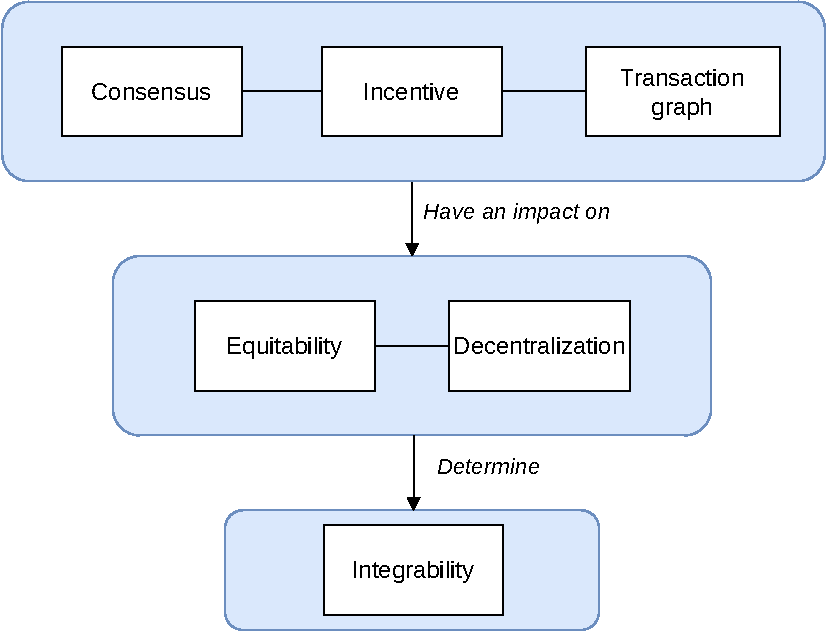
\includegraphics[scale=0.75]{Images/analysis.pdf}
\caption{Criteria used for integration suitability - schematized}
\label{F_analysis}
\end{figure}
To determine whether a DLT instance can integrate properly with the usage control system, we consider two properties of distributed ledger features: decentralization and equitability. These properties are directly influenced by other ledger features which are the basis of our analysis: 1) the consensus method; 2) the incentive to contribute to the network; 3) the transaction graph structure. The method of analysis is schematized in Figure \ref{F_analysis}.
\emph{Equitability} describes the possibility for every user to have a fair part in the decision-making and consensus processes. Particularly, it includes devices with poor computation or storage capacities. This property ensures small devices in the network have an actual impact, and that a small fraction of users do not monopolize the power in the network.
\emph{Decentralization}, besides providing performance and security benefits, is an interesting property to assess the integration suitability. Indeed, decentralization partially reflects the above-mentioned equitability. A fully decentralized network is likely to rely on local consensus to make decisions, which gives a bigger impact on participating devices~\cite{Popov2020, Steen2020}. %In contrast, centralization
Decentralization can take several forms, all expressing power asymmetries~\cite{Bodo2021}:  %. In distributed ledgers, centralization can take two forms~\cite{Bodo2021}: 
1) decentralization in the governance; 2) decentralization in terms of power, where nodes, or more likely node aggregates, have disproportionate power over the rest of the network. For instance, the proof of work consensus method gives power to the most powerful mining pools, while the proof of stake creates another form of centralized capital power. Highly centralized governance is often a prerequisite for a distributed network to work, which means a network can be highly centralized regarding only one centralization aspect, i.e., governance or power, but not the other. 
% The fairer and the more decentralized the network, the stronger the integration. 
The integration is more relevant as equitability and decentralization increase.
The distributed ledger features have an impact on these two properties of equitability and decentralization. To determine the characteristics that favor or hinder integration, three categories of features are next analyzed. 

\textbf{Consensus method.}
Consensus methods are very diverse, but the following are considered in our analysis:

\begin{itemize}
    \item \emph{Proof of Work}: due to computation concerns, a challenging computation race will exclude low-power devices from participating in the consensus. Even though the UCS could make a moderate profit while fulfilling its role, it is not an interesting application for our integration project; 
    \item  \emph{Proof of Stake}: PoS better fits the IoT computational requirements, but has several drawbacks for integration. First, a device can not contribute to the consensus unless it has a stake. Sensors in particular do not have the motivation or the possibility to hold a cryptocurrency asset, either for the consensus or to make transactions~\cite{Raghav2020}. The proof of stake also tends to centralize the network in the hands of a few users, either the delegates (DPoS) or the richest users. Equitability is therefore not achieved with this consensus method. Integrating the UCS in a distributed ledger based on PoS is not relevant, as devices can not contribute to the network;
    \item \emph{Proof of Authority}: PoA, contrary to the proof of stake, does not require holding a cryptocurrency asset. Nevertheless, PoA, by delegating the power to a few nodes considered trustworthy, limits the possibility to integrate the UCS components;
    \item \emph{Proof of Elapsed Time}: in PoET, miners are chosen at random using timers. This consensus method ensures equitability. In this setting, the components of the usage control system could contribute to the consensus, and integration is relevant. However, PoET is limited to private ledgers, as users must first join the network and gain a membership certificate to be allowed to start the timer; 
     \item \emph{Practical Byzantine Fault Tolerance}: all nodes take part in the voting process with equal power, providing the equitability property. Besides, this consensus method is suitable for the IoT but only on private ledgers due to scalability issues in terms of the number of users, as it causes high network overhead~\cite{Salimitari2020}. 
     \item \emph{dPBFT}: \sul{delegating the consensus process to a smaller subset of nodes centralizes partly the network and reduces equitability, but the delegates are chosen by the nodes. The communication overhead is also reduced.}
\end{itemize}

Relying only on consensus methods, it appears that only the practical byzantine fault tolerance (PBFT and dPBFT) and the proof of elapsed time (PoET) are suitable for integration, but both are used only in private settings. This explains why the related works (cf. Section \ref{S_state_of_the_art_ucon_dlt}) mostly focus on private ledgers when the requirements for the IoT use cases are not considered. 

\textbf{Incentive.}
Most consensus methods rely on a financial incentive to encourage users to contribute to the network. The proof of work rewards the miner when it adds a block to the ledger, while the proof of stake rewards the users when they stake their cryptocurrencies for network security. However, rewards have negative side effects. When using a proof of work, it not only encourages miners to contribute to the network but also to group in mining pools. This phenomenon is the cause of the centralization of the network and users can no longer act independently~\cite{Ketsdever2019}. In proof of stake networks, the staking reward incentives create the \emph{Nothing at Stake} issue. 
When a fork occurs, i.e., when two versions of the ledger are competing, the validators have an interest in maintaining both versions to avoid taking the risk of maintaining the wrong one and earning worthless rewards~\cite{Ketsdever2019}. 

In the Internet of Things context, where small devices with energy constraints are involved, the contribution to the network may not be conditioned by financial incentives. IoT-oriented projects would rather focus on operational and energy savings, in particular for battery-powered devices. This is the case for IOTA, which does not introduce any kind of financial rewards for operating a node or validating transactions. The usage control system, as a security device, does not contribute to the network for financial rewards but seeks to deliver fast access decisions at the minimum cost.

\textbf{Ledger type.} Considering consensus methods, it appears that private blockchains are more suitable for integration than public blockchains. However, directed acyclic graphs have several properties of interest, among which some significantly ease the integration process. The removal of gateways in directed acyclic graphs enables the users to push their transactions directly to the network. This is also true for the usage control system, which may actively contribute to the network. The overall metrics of directed acyclic graphs enable more users to contribute to the network. The usage control system can make its decisions faster by processing the transactions locally.
 
 
 \textbf{Selection of the suitable distributed ledgers.} 
 To sum up, the possibility to integrate usage control with distributed ledgers is mostly determined by the equitability of the protocol and its decentralization. Three main criteria have a direct impact on equitability and decentralization: the consensus method, the incentive and the transaction graph.
 
 The consensus method has a direct impact on the possibility for small devices to contribute to the network. The incentive is paramount as well because usual financial incentives tend to centralize the network. Finally, the ledger type, either a blockchain or a directed acyclic graph, has a deep impact on the network features. Since DAGs are meant to allow users to push and check transactions themselves, they enable the contribution of the usage control system to the network.
 
  According to this classification, summarized in Table~\ref{tab:classification}, it is possible to depict two categories of fitting technologies, both without a financial incentive: directed acyclic graphs and private blockchains. However, only directed acyclic graphs consider the large-scale IoT requirements, while private blockchains are not scalable and do not have cryptocurrencies. Consequently, \emph{we will consider directed acyclic graphs} for the integration of usage control in the following. 

\begin{table*}
\setlength{\extrarowheight}{12pt}
 \begin{center}
 \begin{scriptsize}
\begin{adjustbox}{angle=90}
\begin{tabular}{ |c|c|c|c|c|c|c| } 
\hline
Parameter & Instance & IoT Suitable & Equitability & Decentralized* & Integration & Notes\\
\hline
\multirow{5}{4em}{Consensus} & PoW & \xmark & \xmark  & \xmark (.pow) & \xmark & Compute-intensive\\ 

& PoS & \xmark & \xmark & \xmark (.pow) & \xmark & Stake needed\\ 

& PoA & \xmark & \xmark & \xmark & \xmark & Similar to PoS \\

& PBFT & \cmark & \cmark & \cmark & \cmark & Private blockchains only \\

& dPBFT & \cmark & \cmark & \cmark & \cmark & Less equitable, low communication overhead \\
& PoET & \cmark & \cmark & \xmark (.gov) & \cmark & Private blockchains, relies on Intel SGX\\
\hline
\multirow{3}{4em}{Incentive} & Financial & \xmark & \xmark & \xmark & \xmark & Deterrence for small devices \\ 
& Savings & \cmark & \cmark & ? & \cmark & Incentive for small devices\\ 
\hline
\multirow{3}{4em}{Ledger} & Private blockchain & \cmark & \cmark & \xmark (.gov) & \cmark & Promising but scalability, currency issues\\ 
& Public blockchain & ? & ? & ? & ? &  Very diverse, not determining \\
& Directed acyclic & \cmark & \cmark & \cmark & \cmark & Significantly favors integration\\
\hline
\end{tabular}
 \end{adjustbox}
\captionof{table}{DLT parameters and their impact on integration. Question marks (?) mean the parameter is not determining. \\ *Decentralized can take several forms, governance (.gov) or power asymmetries (.pow)}
\label{tab:classification}
 \end{scriptsize}
 \end{center}
 \end{table*}

\subsection{Integration benefits}
\label{ss_integration_benefits}

A logical way to integrate the usage control system with a distributed ledger based on a DAG is to run a node. Nodes are indeed critical components of distributed ledgers. They differ depending on the technology, but their purpose is at least to check the validity of transactions. The usage control system could run a node with the following expected benefits for itself:

\begin{itemize}
    \item \emph{disintermediation}: running a node avoids relying on a third party. The bandwidth is secured for the node transactions without delay. Usage control with policies based on transactions is faster, based on the local ledger analysis;
    \item \emph{storage control}: the node may keep all transaction records to enforce the policies if necessary. Nodes usually rely on local snapshots to reduce the size of the local ledger;
    \item \emph{node configuration}: the node can be configured to adjust both security and performance parameters to the UCS needs;
    \item \emph{network security}: the UCS will contribute to the ledger verification, reducing the probability of failure resulting from a low number of nodes \cite{Khacef2021}. Besides, a higher number of nodes makes some attacks harder, such as the 51\% attack \cite{Aponte2021};
    \item \emph{throughput increase}: the UCS increases the throughput as it pushes transactions on the network, due to DAG properties;
\end{itemize}

% Running a node bolsters the network, increasing security regardless of the ledger, and performances for directed acyclic graphs. Indeed, in DAGs, the throughput increases with the number of users.

To fulfill its mission, the usage control system has to monitor system and network calls, which is an intrusive process. \emph{Transparency} and \emph{auditability} are paramount in this context. 
Transparency in usage control can be considered as the fact that the usage control operations, e.g., allowing access or preventing dissemination, are communicated to others, while auditability anticipates the storage of these usage control data for a future audit. 
Transparency and auditability can be achieved by writing usage control data on the ledger such as the operations performed by the UCS on the users. Auditability incites the usage control system to behave correctly, as any misbehavior will be recorded publicly on the ledger. 

\subsection{Integration methodology}
\label{ss_integration_methodology}

The integration methodology concerns two aspects: the global system architecture, considering how the usage control system can integrate the distributed network, and data protection, as data written on the ledger becomes visible and exposed to privacy risks.

\textbf{Integration as a Node.}
Directed acyclic graphs, by design, alleviate the requirements on nodes to maximize the number of devices contributing to the network. Therefore, the usage control system itself can deploy a node and push transactions itself. By deploying a node, the usage control system will 1) push transactions including some related to usage control use cases, accelerating the access decision process; 2) prioritize its transactions on the network, avoiding a potential queue; 3) store a local copy of the ledger, to process the ledger faster when necessary for its access decision. The integration model is represented in Figure~\ref{F_peripheral_vs_integrated}, showing the links between the UCS, the nodes, and the monitored users. Data can be partially written on the public ledger as long as they do not create inference risks, as described in the following.

\begin{figure*}[t]
\centering
 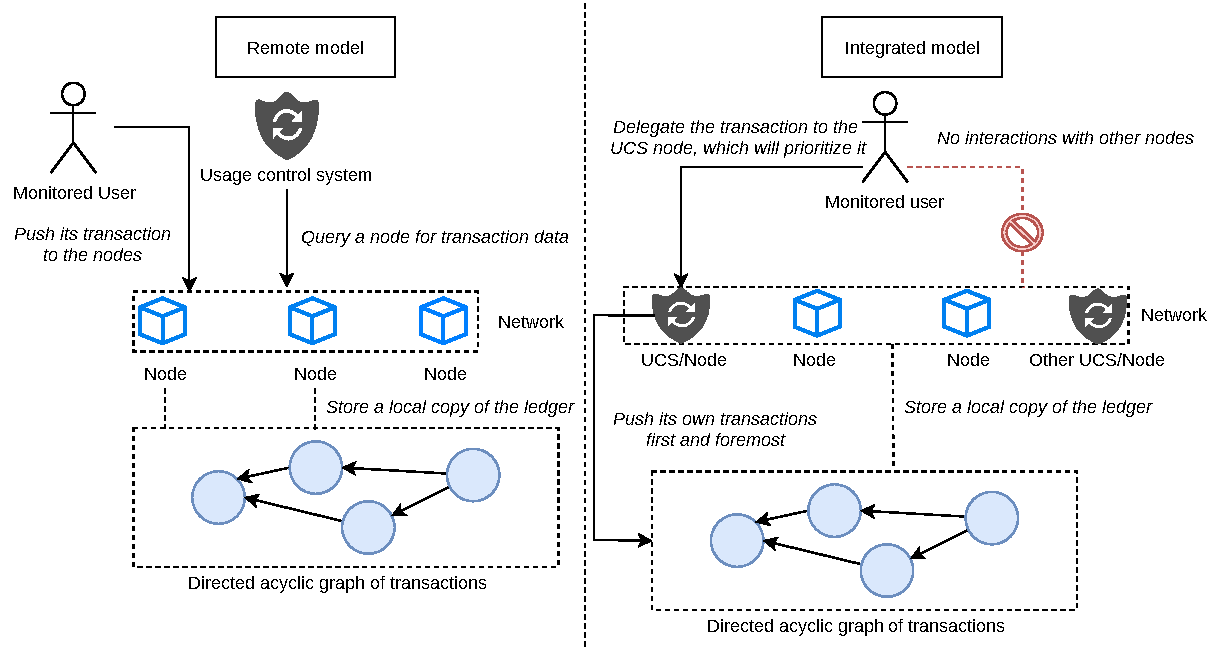
\includegraphics[width=\textwidth]{Images/remote_vs_integrated.pdf}
\caption{Differences between the remote model and the integrated model when using directed acyclic graphs.}
\label{F_peripheral_vs_integrated}
\end{figure*}

\textbf{Data management.}
For public ledgers, one key motivation for integration is the capacity to write immutable data on the ledger for transparency purposes (cf. Section~\ref{ss_integration_benefits}). Data must be classified to determine whether they can be displayed publicly or not. Data can be of four types, summarized in Table~\ref{tab:storage}: 

\begin{itemize}
    \item \emph{protected data}: data whose access is monitored by the UCS;
    \item \emph{usage control data}: data concerning the usage control, including the processes performed by the UCS as well as the results of the evaluation;
    \item \emph{users' data}: data needed by the UCS about the users, such as their attributes to make access decisions;
    \item \emph{metadata}: data about the other data, e.g., data that states the kind of processed attributes, but not the content of the attributes.
\end{itemize}

Protected data must not be stored in clear text on the ledger, and can either be encrypted on the public distributed ledger or stored in a distributed database. However, encryption produces computational overhead and the management of encryption keys is a real issue in large-scale contexts; that is why we resort to using a database management system. Usage control data describe the operations performed by the usage control system on the users. They are composed of a data identifier, the pseudonyms of the users and the action performed. They are published on the public ledger for transparency and auditability purposes. Data about users, such as their attributes, are needed only by the usage control system and are stored in the database. Finally, metadata is published on the ledger, such as timestamps and data identifiers to keep track of the data. Metadata can pose a \emph{detectability threat} when revealing its existence can lead to privacy issues, even without providing the actual content of the data, e.g., knowing the existence of a police record associated with an identity, without the content inside the record, is a sensitive information. Metadata must therefore be processed carefully, using a privacy threat analysis framework such as LINDDUN~\cite{Deng2011}.

%%%%
\begin{table}[ht] 
    \centering
    \resizebox{0.55\textwidth}{!}{%
      \begin{tabular}{|c|c|c|c|c|}
        \hline
        Data type & Data storage \\ 
        \hline
        Protected & Database \\ 
        Users' data & Database \\
        Usage control & Directed acyclic graph \\
        Metadata & Directed acyclic graph*\\
        \hline     
      \end{tabular}}
      \caption{Data types and their respective storage area \\ * If detectability is not an issue}
      \label{tab:storage}
    \end{table}  
    %%%%
\section{Performance evaluation}
\label{S_performance_evaluation}

In this section, we detail the results of a performance evaluation conducted on IOTA to demonstrate that the integration is efficient and to assess its estimated performance outcomes. To this end, we will measure the time needed for the UCS to make an access decision in the integrated setting compared to the remote node setting.

\subsection{Testbed}
\label{ss_testbed}
 \textbf{Testing environment.} To assess our contribution, we test our integration using the IOTA technology (cf. Section \ref{S_iota_dlt}). Since data are partially stored off-chain (cf. Section~\ref{ss_integration_methodology}), we relied on a \emph{Cassandra} distributed NoSQL database as decentralized storage. Cassandra is \emph{horizontally scalable}, meaning it easily handles increasing traffic demands by adding more machines~\cite{Silva2021}. Cassandra also works on low-power clusters, which is particularly suitable for the Internet of Things~\cite{Silva2021}.
 The IOTA node relies on \emph{Hornet}, a community-driven IOTA node software written in the \emph{Go} language. The usage control system is written in Java. The usage control policies are defined by the users and written using the XACML language~\cite{Godik2003}. An example of an XACML policy is provided in the appendix (Figure \ref{listing:XACML_policy}). During the tests, policies are not specified by users, but automatically derived for convenience.

\textbf{Network selection.}
IOTA has a public development network called \emph{devnet} for testing. The devnet has free tokens and is meant for testing. The public devnet could be convenient because its network is already deployed and designed to conduct tests, in particular, to measure resistance in high-load scenarios. However, it has significant drawbacks for testing. First, the network is subject to complete overhauls with no backward compatibility, preventing the reproduction of the tests conducted in our experiments on the same network. In particular, the introduction of IOTA 2.0 will lead to the removal of the IOTA 1.0 testing network. Second, the network is public, it is not possible to control the network topology including the number of nodes.

Consequently, the tests on the public network are not sufficient to ensure the efficiency of integration.
To ensure our tests can be reproduced, we deploy a \emph{private Tangle} instead. This methodology has been used by Dong \emph{et al.} \cite{Dong2019} to benchmark different DAGs including IOTA. Each node is deployed on AWS instances and constitutes a part of a private IOTA network. The network architecture of the private Tangle with AWS instances is given in Figure \ref{F_network_architecture}, for 5 nodes.

\begin{figure}[t]
\centering
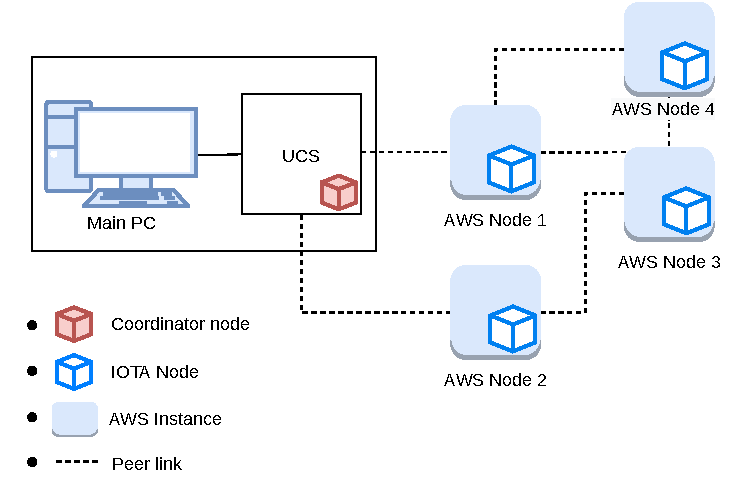
\includegraphics[width=0.8\textwidth]{Images/AWSarchitecture.pdf}
\caption{Private Tangle architecture with AWS instances - 5 nodes. Each instance runs an IOTA node, and a PC runs the Coordinator node to orchestrate the network.}
\label{F_network_architecture}
\end{figure}

\textbf{Nodes settings.} The tests are conducted using AWS t2.micro instances with 8 Gio\footnote{1 Gio=1024 Mo} storage capacity, 1 vCPU and 1 Gio RAM, consistent with the Internet of Things constraints. Another computer is used to run the usage control system, with better storage and computational power: 8Go of RAM memory, 32Go of storage and 4 CPUs. The nodes are located in Amazon's default US East (North Virginia) zone. Each Hornet node \emph{when running on the private Tangle} uses the default spammer, spamming 5 messages by second for each node. Spamming is a desired behavior, as it theoretically speeds up the transaction validation in IOTA (cf. Section \ref{S_iota_dlt}).

\subsection{Methodology}
\label{ss_methodology}

\begin{table}[h]
    \resizebox{\textwidth}{!} \\
        
        & Remote & 1020$\pm21$ ms & 85 ms & \\
        \hline
        \multirow{2}{4em}{5 nodes} & Integrated & 61$\pm3$ ms & \xmark & \multirow{2}{4em}{93.59 \%} \\
        
        & Remote & 868$\pm38$ ms & 84 ms &\\
        \hline
        \multirow{2}{4em}{7 nodes}
        
        & Integrated & 66$\pm3$ ms & \xmark & \multirow{2}{4em}{92.31 \%}  \\
        
        & Remote & 773$\pm16$ ms & 86 ms & \\
        \hline
        \multirow{2}{4em}{10 nodes}
        & Integrated & 58$\pm3$ ms & \xmark & \multirow{2}{4em}{93.77 \%}\\
        & Remote & 845 ms$\pm32 ms$ & 86 ms & \\
        \hline      
      \end{tabular}}
      \caption{Measures of transaction time (averages) for each configuration with different networks sizes}
      \label{tab:measures}
    \end{table}   

\textbf{System model.}
The agents of the system can be summarized as follows. First, the \emph{data providers} that sell data collected from their devices. Then the \emph{data buyers} pay a certain amount of cryptocurrency to be granted access to these protected data.
 The \emph{usage control system} (UCS) is responsible for monitoring the data access rights and for preventing dissemination, based on data buyers' attributes and actions. 
In particular, it processes the transactions on the \emph{distributed ledger} to grant access if the payments are duly performed. A Cassandra \emph{distributed database} shared between the data providers stores the protected data. \emph{Network nodes} validate the data buyers' transactions and propagate them to the other network nodes. The system model is depicted in Figure~\ref{F_system_model}.

\begin{figure*}[t]
\centering
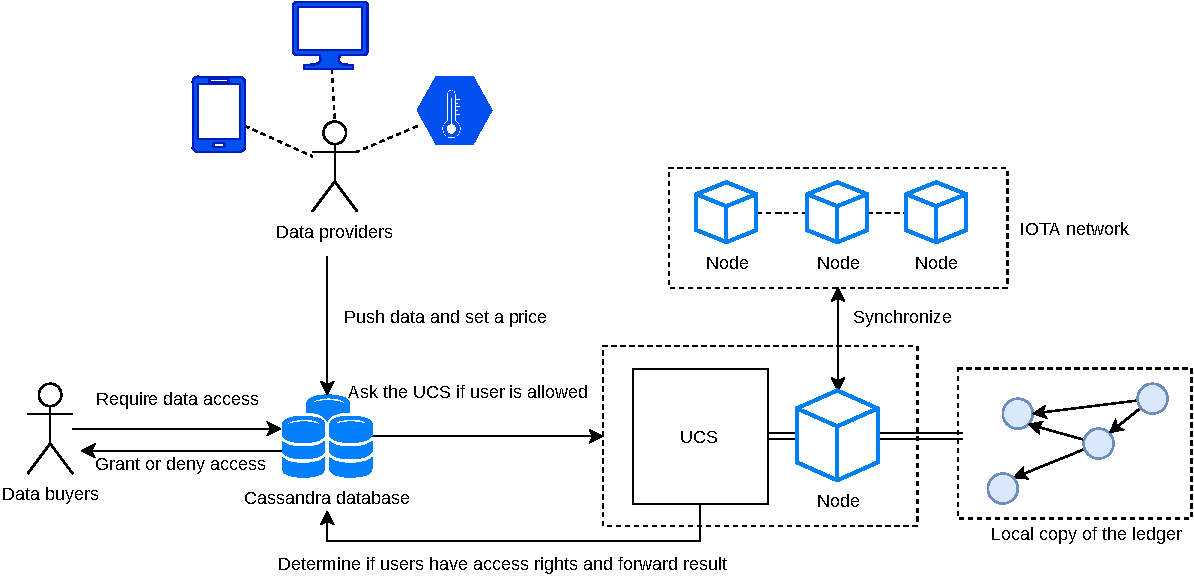
\includegraphics[width=\textwidth]{Images/system_model.pdf}
\caption{Interactions within the system model during the pre-access phase}
\label{F_system_model}
\end{figure*}

\textbf{Workflow.}
To determine which calls are of interest to assess performance outcomes of integration, the system and network calls needed for granting or denying access are detailed and classified into two categories according to the intensity of computations required,
as depicted in the sequence diagram of Figure \ref{F_sequence_iotj}. Either a call is  \emph{computationally-intensive} (1) or \emph{lightweight} (2).
This notion is comparative, such that lightweight calls are not time-consuming compared to computationally-intensive calls. 
The workflow following an access request is as follows. First, the data buyer requires access to data by sending an \texttt{accessRequest} along with its user identifier. 
Then it sends a \texttt{transaction} to an IOTA node to perform the payment. 
This node checks if the transaction is correct, e.g., no double spending, by checking it against the local state of the ledger.
If the transaction is indeed correct, the node computes a light proof of work only to prevent spam. The node then forwards the transaction to the rest of the network, using the \texttt{push} call.
The UCS then begins the monitoring of the access and sends a \texttt{requestPolicy} to its policy store, fetching the XACML policy specified by the data provider.
The UCS asks for attribute values of the data buyer (\texttt{requireAttributes}) to be able to check policy compliance. The attribute values are used for data access control, but also include values resulting from the analysis of network calls to monitor the information flow.  
When the UCS receives the attributes from the data buyer (\texttt{sendAttributes}), it fetches the transaction status on the network by calling \texttt{fetchTransaction}, then determines the policy compliance ( \texttt{checkPolicy}) to make an access decision. If the user is authorized to access the data, the UCS sends a \texttt{ grantAccess} call to the Cassandra data provider database and notifies the data buyer with a \texttt{notifyAccessResult}. Following the \texttt{grantAccess} call, the data provider sends the requested data to the data buyer with the \texttt{sendData} call.
The data buyer is monitored by the UCS for the ongoing obligations and ongoing conditions (cf. Section \ref{ss_ucon_elementaries}) with \texttt{ongoingMonitoring} calls. For convenience, only one call is represented in the sequence diagram (Figure \ref{F_sequence_iotj}),
but the monitoring usually requires numerous calls due to the continuous nature of the monitoring. The monitored data buyer must reply to \texttt{ongoingMonitoring} with \texttt{sendOngoingData} so that the UCS can make its access decisions and interrupt access if the policy is violated.
The UCS writes usage control logs and metadata for transparency on the ledger while considering privacy threats (cf. Section \ref{ss_integration_methodology} and Table \ref{tab:storage}) by calling \texttt{writeAccessLogs}. The access is finally revoked by the UCS with \texttt{revokeAccess}, should the data user request it or contravene the data provider's policy.

\begin{figure*}[ht]
\centering
 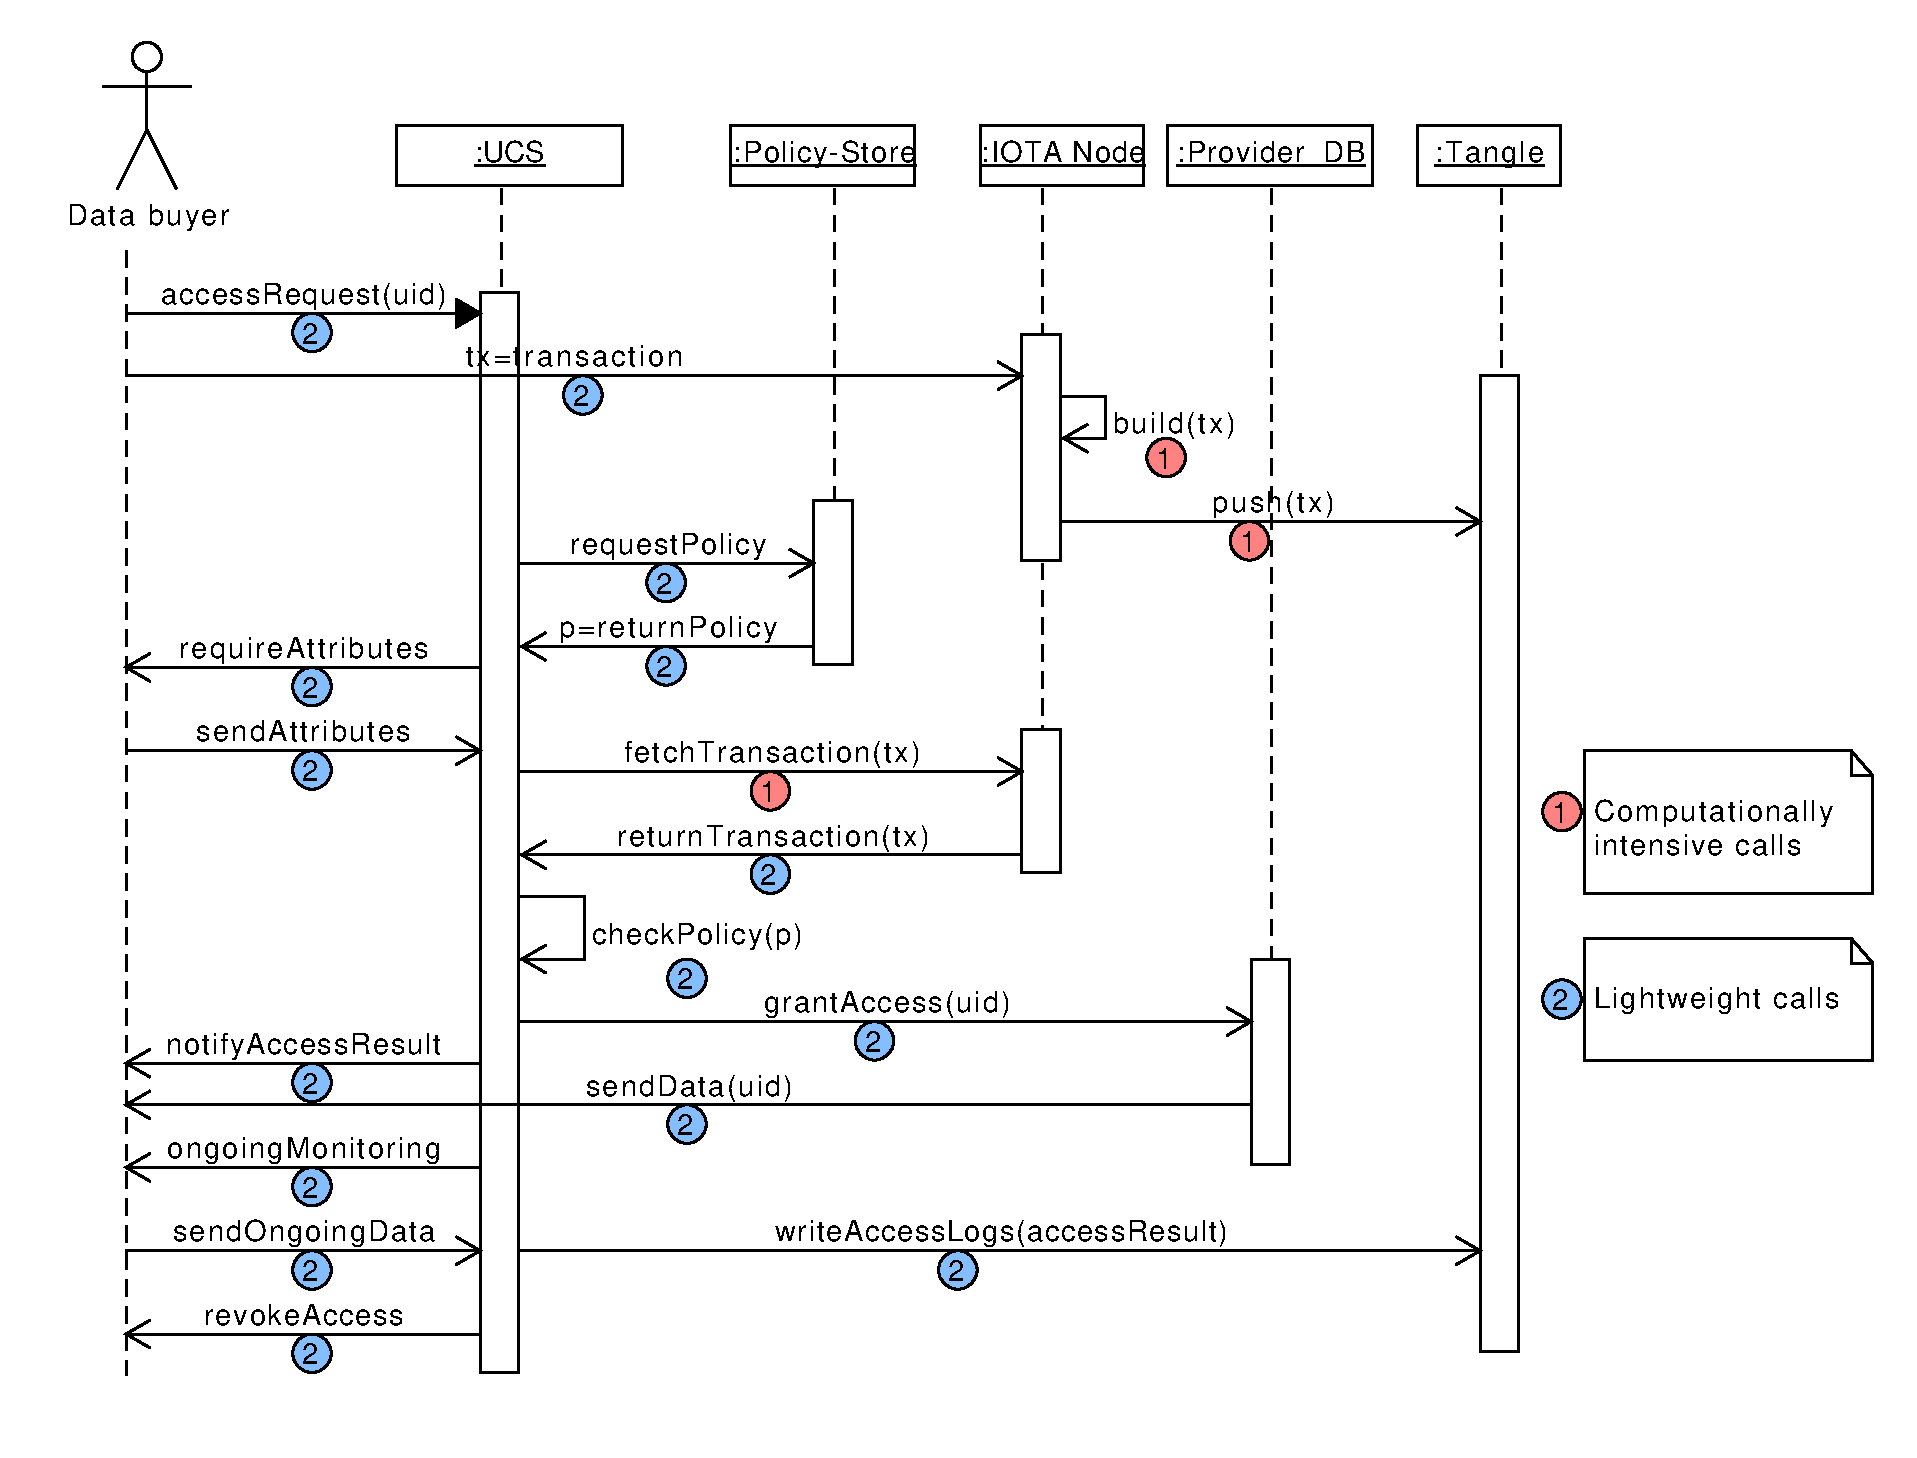
\includegraphics[width=\textwidth]{Images/sequence_iotj.pdf}
\caption{Sequence diagram for pre-access and ongoing access - UCS not integrated with IOTA}
\label{F_sequence_iotj}
\end{figure*}

\textbf{Measured calls.}
Only the \texttt{build}, \texttt{push} and \texttt{fetchTransaction} calls will be measured as the only computationally intensive calls. They are referred to as \emph{transaction time}. Our first guess would be to also include
the \texttt{checkPolicy} calls; however first tests showed that a
policy with 1000 rules takes an average 7 ms to be evaluated (1500 samples), which is lightweight compared to the transaction time. Other calls are also lightweight when measured.
The three calls \texttt{build}, \texttt{push} and \texttt{fetchTransaction} are the most time-consuming for the reasons detailed next. To build and push a transaction, the node must compute a proof of work and check that the transaction is consistent with its known ledger state.
The \emph{fetchTransaction} call is time-consuming due to several varying parameters: 1) the node is processing other transactions which delays the \texttt{fetchTransaction} call by adding it to its processing queue; 2) the (physical) distance between the node and the UCS without integration, which creates network latency; 3) the time needed to query the ledger of the node, which increases with the number of simultaneous requests.

\textbf{Transaction time.}
To demonstrate actual performance improvements, we measure the time needed for a transaction to be validated and pushed to the network, and the time required to fetch the transaction from an IOTA node. These operations are respectively the calls \texttt{build}, \texttt{push} and \texttt{fetchTransaction} of the sequence diagram of Figure \ref{F_sequence_iotj}. The \texttt{build} and \texttt{push} calls are grouped under a single API call in the Java IOTA library and correspond to only one common measure.
Tests are conducted in the two different configurations, respectively the remote and the integrated settings: (1) the UCS interacts with a remote IOTA node running in an AWS instance; (2) an integrated node that runs both the UCS and an IOTA node concurrently, as illustrated in Figure \ref{F_peripheral_vs_integrated}.
For each test, 1500 samples ($N=1500$) are used and confidence intervals are given with a 95\% confidence level.

\subsection{Results}
\label{ss_results}

The results of experimental measurements are summarized in Table~\ref{tab:measures}. For convenience, only the experiments with 5 nodes $N=5$ are first discussed. We then detail the impact of the number of nodes on the results and provide further explanations.

\textbf{Remote setting}. When the UCS interacts with a remote node, the \texttt{build} and \texttt{push} calls need an average $\overline{t}_{transaction, r} =868\pm 31 ms$ with 5 nodes in the network. Building and pushing a transaction requires a minimum $m_{r}=646 ms$ and a maximum $M_{r}=7649 ms$. This wide range is caused by nodes which are often desynchronized and have to update the state of the ledger before pushing their transactions. 
Additionally, the UCS has to recover the result of the transaction requiring an additional $\overline{t}_{fetch, r} = 84\pm0.38ms$.

\textbf{Integrated setting}. When using an integrated node on the UCS device, the transaction time improvements are significant. Indeed, the \texttt{fetchTransaction} call does not involve any network calls and requires less than 1 ms to be completed when measured. Our own transactions are prioritized on our node, substantially decreasing the time to complete the \texttt{build} call. The average time needed to \texttt{build} and \texttt{push} a transaction drops to $\overline{t}_{transaction, l}=61\pm2.86ms$.

\textbf{Number of nodes.} As the number of nodes increases, the impact of integration in percentage remains steady, varying from a 92.31\% to a 94.12\% transaction time decrease. The transaction time in our integration scheme is consequently 13 to 18 times faster compared to the remote node setting.

The time required to build and push transactions decreases before 7 nodes, then starts to go up when using 10 nodes. Firstly, the number of messages spammed increases with the number of nodes. We can therefore observe the expected behavior of IOTA \cite{Popov2017}: as the number of transactions per second increases, transactions are validated faster. Secondly, when reaching 10 nodes, there are approximately 50 messages spammed per second as each node spams 5 messages per second. There are two possible explanations for this behavior. First, the network could saturate due to the Coordinator milestones validation.
This issue is well-identified by both the IOTA foundation and academics \cite{Conti2022, Wang2022} and is the motivation for the development of IOTA 2.0, willing to remove the Coordinator. However, the Coordinator runs on the same device in both integrated and remote settings, but the transaction time does not increase for 10 nodes in the integrated setting. Therefore, we can conclude that it is not the Coordinator that saturates, but the remote node used for the testing. Indeed, the nodes running on AWS are resource-constrained, and processing 50 transactions per second is time-consuming for an instance with 1 Gio of RAM and 1 vCPU.

\section{Privacy evaluation}
\label{S_privacy_evaluation}
 In this section, we conduct a privacy threat analysis, to highlight the risks for the users either selling or buying data in the system as described in Section \ref{ss_methodology}. Based on this analysis, we then detail how usage control mitigates the different privacy risks.

\subsection{Threat model} The \emph{usage control system} is considered \emph{honest-but-curious}. It fulfills its usage control tasks but may be interested in collecting undue data about the users it monitors. This behavior may be financially motivated, i.e., to sell the users' data afterward. In particular, the UCS has an interest in gathering the system calls and network calls of the monitored users, both carrying valuable, privacy-sensitive data.

\emph{Data buyers} and \emph{data providers} are considered honest-but-curious as well. Notably, data buyers try to infer more data from the protected data they buy, but do not try to bypass the UCS monitoring or to compromise the database.
The \emph{Cassandra distributed database} is considered as trusted and not compromised.

\subsection{Privacy risks}
\label{ss_privacy_risks}

 The \emph{LINDDUN privacy threat modeling framework} \cite{Deng2011} (cf. Section \ref{ss_privacy_threat_modeling}) is used to describe the 
 different privacy risks faced by data buyers and data renters.
\textbf{Items of interest.} Items of interest (IOI) in LINDDUN refer to any data element, including users' personal data or transaction data, that is considered privacy-sensitive. It is paramount to exhaustively identify which items are of interest before conducting the privacy threat assessment, to ensure the full listing of the threats. Items of interest can be subjects, messages, actions or data. \sul{In scenarios involving transactions, the items of interest can be}:
\begin{itemize}
    \item the geolocated protected data generated by data providers;
    \item the transaction data, including but not limited to users' addresses and transaction values;
    \item users' data, i.e., data buyer and data provider personal data;
    \item usage control data, such as the results of access requests;
    \item metadata, such as the time the data was created or added to the Cassandra database, that can be used to infer other data.
    \item data buyers, data providers, the UCS and the Cassandra database, i.e, subjects;
    \item network messages between the subjects, and the messages between the UCS components (cf. Section \ref{ss_ucon_architecture});
    \item actions carried out by the subjects, such as an access request by the data buyer, entry insertion on the database by the data provider or the beginning of an access request evaluation by the UCS.
\end{itemize}

In the following, transaction data are ignored, as preserving privacy in distributed ledgers is a specific, orthogonal research topic. Legal compliance in particular is troublesome for distributed ledgers \cite{Haque2021}, and privacy-enhancing technologies have been designed to address privacy threats, such as cryptocurrency mixers for linkability \cite{Sarfraz2019}, \cite{Glaeser2022}.


\textbf{Linking (L).} Linking occurs when two \emph{items of interest} are associated to learn more about an individual or a group. Due to the diversity of agents and technologies involved, linking threats are numerous in the electricity consumption prediction scenario:

\begin{enumerate}
    \item linkage between protected data and its owner (user data). The location in the protected data can be used to facilitate the re-identification of the data providers (I);
    \item linkage between a data buyer and a data provider. It simplifies re-identification when one of them is identified (I);
    \item linkage between metadata and usage control data, as both are written on the ledger.
\end{enumerate}

Linking leads to other identifying (I), detection (D) and non-repudiation (N) threats and is triggered by data disclosure (D) - the more data available, the more likely are linking threats.

\textbf{Identifying (I).} Identification is occurring when an attacker learns the identity of an individual, breaking its anonymity or pseudonymity. This threat distinguishes \emph{identified data} where the identity is explicitly maintained, and \emph{identifiable data} which enables to derive the identity indirectly. Users' attributes, e.g., IP address or processed by the usage control system to make an access decision can be used to infer the user's true identity. In the scenario, the risks are to re-identify data buyers and data providers, using protected data, usage control data or metadata.

\textbf{Non-repudiation (N).} Non-repudiation, in LINDDUN privacy threat assessment, is the ability to attribute a claim to an individual. For example, the impossibility for a data buyer to deny they bought and accessed protected data, or for data providers to deny they generated a given data, are non-repudiation threats.

\textbf{Detecting (D).} Detecting is the ability to deduce the involvement of an individual in an action with observation. Detecting does not require being able to read the actual data. Knowing that the data exists is enough to infer more sensitive information. Detecting can be done by observing \emph{communications} or \emph{application side-effects}. Detecting threats in the electricity consumption prediction scenario includes: 
\begin{enumerate}
    \item detecting that a user is monitored by analyzing the communications of the UCS. An attacker learns that the user has likely bought valuable data;
    \item detecting what are the protected data and where they are disseminated, without the actual content of the data, by analyzing the UCS logs;
    \item detecting users' attributes by intercepting the communications between the policy information points (PIP) and the context handler (CH) (cf. Section \ref{ss_ucon_architecture});
\end{enumerate}

\textbf{Data disclosure (D).} Data disclosure is the
immoderate collecting, storing, processing or sharing of personal data. This generic threat focuses on four characteristics:
\begin{enumerate}
    \item \emph{unnecessary data types}, if the data granularity or sensitivity is too detailed;
    \item \emph{excessive data volume}, if the amount or the frequency of data processing is too high;
    \item \emph{unnecessary processing}, if the data is processed or disseminated out of necessity;
    \item \emph{excessive exposure}, refers to how widely accessible the data is and to whom the data is shared.
\end{enumerate}

In the energy consumption prediction scenario, data disclosure can occur if a data provider has access to protected data while not fulfilling the policy's conditions, or can disseminate it outside of the UCS monitoring perimeter. Similarly, data disclosure occurs if the UCS collects too detailed data about the data buyers to monitor them.

\textbf{Unawareness (U).} Unawareness occurs when an individual is insufficiently informed and involved in the processing of personal data.
Unawareness occurs in the scenario if the data providers are not informed about the privacy threats they face by
selling their data with associated geolocation. The user may also be unaware of the privacy risks of accepting to be monitored by the UCS, which writes usage control data on the ledger, that are potentially privacy-sensitive (cf. Section \ref{ss_methodology}) 

\textbf{Non-compliance (N).} Non-compliance is the deviation from security and data management best practices, standards and legislation. This risk occurs if the processing of any item of interest is considered unlawful based on the specified policies and the applicable regulations, e.g., GDPR \cite{EUdataregulations2018}. In the scenario, the risks are that although the data provider specifies a policy, it is not properly enforced by the usage control system.
% In particular, users lack \emph{intervenability} in the scenario: once the transaction data
% are written on the ledger, they can not be removed. This is a common issue in distributed ledger, contravening GDPR's articles 16 and 17 - right to rectification and erasure} \cite{EUdataregulations2018}.

% \ul{Another issue is the data \emph{retention time}, which should be limited to the time required to process the data. Yet, the data written on the ledger, i.e., usage control data and some metadata, are stored indefinitely. Besides, the principle of data minimization (article 5)}\cite{EUdataregulations2018} \ul{ requires that only the necessary data be collected and processed. However, in a public distributed ledger like IOTA, all participants have access to all data, including unnecessary or irrelevant data. The GDPR also requires that data controllers and processors ensure the protection of personal data (Article 32)}\cite{EUdataregulations2018} \ul{. Using IOTA, users push the transactions themselves. It is hard to determine who is responsible for compliance. Finally, consent may not be possible or practical (Article 7)}\cite{EUdataregulations2018} \ul{, as anyone can access the data on the ledger without the need for consent}

\begin{table}[ht] 
    \resizebox{\textwidth}{!}{%
      \begin{tabular}{|c|c|c|c|c|}
        \hline
        Threat & Scenario example & Mitigated by the UCS\\
        \hline
        Linking & Link between data owner and buyer & ?\\
        Identifying & Data provider is re-identified & ?\\
        Non-repudiation & Data provider can not deny data generation & \xmark \\
        Detecting & Detect a user is monitored & \cmark\\
        Data disclosure & Protected data dissemination & \cmark\\
        Unawareness & Inference risks of location unknown  & \cmark\\
        Non-compliance & Data provider policy not enforced & \cmark\\
        \hline      
      \end{tabular}}
      \caption{LINDDUN privacy threat analysis, based on the illustrative scenario.\\ (?) marks 
means the threat is only partly mitigated by the UCS.}
    \label{tab:threats}
    \end{table}   

\subsection{Threat mitigation with usage control}
\label{ss_mitigation}

As a privacy-enhancing technology, usage control is designed to address a significant part of the above-mentioned privacy threats. We next detail how these threats are addressed, and which ones can not be mitigated by the UCS. The results are summarized in Table \ref{tab:threats}.


\textbf{Linkability. (?)}
The usage control system has only a partial impact in preventing this threat. Notably, the linkage between metadata and usage control data, which are both unrestricted data available publicly on the ledger, can be accessed without monitoring in the first place. However, the UCS monitors the dissemination and the processing of the protected data, limiting the risks to link them to their owners.

\textbf{Identifying. (?)} Similarly, the usage control system must be able to identify the data buyer to fulfill its mission. While it can prevent users from disclosing \emph{identified data}, it is much harder for it to prevent inference from \emph{identifiable data}.

\textbf{Non-repudiation. \xmark}  To fulfill its task, the UCS needs to ensure that a monitored data buyer can not decline having disseminated the data, or having processed it in an unlawful manner. Therefore, the UCS not only does not guarantee non-repudiation, but also writes usage control data on the distributed ledger, making non-repudiation impossible.

\textbf{Detecting. \cmark} To mitigate this threat, all communications are secured using TLS, notably the communication between the usage control system and the users, the context handler and the PIPs, as well as the context handler and the PEPs. Besides, unless the UCS is compromised, an attacker does not have access to the logs of the UCS.

\textbf{Data disclosure. \cmark} The data processing is monitored by the usage control system, mitigating the \emph{excessive data volume} threat. The usage control system, by monitoring both the information flow and the usage of the data, also prevents \emph{unnecessary processing}. \emph{Excessive exposure} is prevented as part of the access control to the data.

\textbf{Unawareness. \cmark} The usage control system asks data owners to design data policies themselves, directly addressing the unawareness threat.

\textbf{Non-compliance. \cmark} The usage control system monitors the data buyers, stopping them from processing the data unlawfully. The usage control system, considered honest-but-curious, enforces the proper usage control policy specified by the data provider.


Usage control addresses four categories of threats directly, i.e., detecting, data disclosure, unawareness and non-compliance. Due to the diversity of the data and agents considered, linking and identifying threats are only partially mitigated. Only the non-repudiation threat is not considered by usage control.

\section{Conclusion}
\label{S_conclusion_integration}

In this chapter, we introduced and evaluated the integration of usage control with distributed ledger technologies. After identifying the 
possible compatible DLTs (Section \ref{ss_integrability_criteria}), we developed a proof of concept using IOTA before conducting performance tests (Section \ref{S_performance_evaluation}).
\sul{Even though similar works exist in the state of the art that propose the integration (also referred to as incorporation) of usage control with blockchains, the integration is always conducted in private blockchain settings. 
The work in this thesis therefore comes as a novelty, by studying the integration process itself, and by identifying DAG-based distributed ledgers as 
potential permissionless solutions for large-scale IoT networks.} 

While this chapter focused on usage control, the integration principle can be generalized to any system that requires to process
distributed ledger transactions and that can be deployed on a node. 
The network security always benefits from having more nodes (cf. Section \ref{ss_integration_benefits}).
For example, the mixing services can benefit from integration (cf. Section \ref{ss_obfuscation_coin_mixing_merge_avoidance}), especially
when decentralized as used in Chapter \ref{C_solving_trilemma} as the mixing peers can be numerous. 
Similarly, a device will benefit from deploying a node if it has to analyze the transaction, which is the case for the UCS so as to monitor access. In the next Chapter \ref{C_formalism}, we will digress from practical optimization aspects and discuss modeling. We will see the limitations of the current usage control formalism and how it can be better adapted to the Internet of Things.  
\newpage \ \newpage
%--------------------------------------------------------------------------------

\chapter{Modeling Distributed Data Usage Control}
\label{C_formalism}
\minitoc
\section{Introduction}
Data usage control enables data owners to enforce policies for their data, 
by defining authorizations, but also obligations, which are actions to be performed before, during or after being granted access, and conditions bearing on the system and environment attributes such as the time or the system load.
Information flow control (IFC) is a security mechanism that regulates the movement of data within 
a system or network, to prevent undue dissemination of the data \cite{Denning1976}. A decentralized version called \emph{Decentralized Information Flow Control} (DIFC), was introduced by Myers and Liskov in 1997. Contrary to traditional IFC, it enables users to define policies individually or as a group without relying on a central entity. Data owners add security labels to the data directly, to indicate who is allowed to read the data \cite{Myers1997}.
While usage control and information flow control are two different technologies, they are used jointly by modern usage control systems (UCS)~\cite{Harvan2009}. Therefore, recent models~\cite{Kelbert2018, Fromm2020} tend to encompass both aspects as usage control needs to prevent dissemination in areas outside of the monitoring scope. Introducing usage control can therefore lead to unclear statements, as it is hard to distinguish whether usage control refers to classic usage control, i.e., UCON and derived models, or classic usage control with information flow control. For disambiguation, the following terminology is used
in this chapter:
  
\begin{itemize}
    \item \emph{data usage control} (UCON): refers to the policies which define the users' rights to access data, based on authorizations, obligations, and conditions;
    \item \emph{information flow control} (IFC): refers to the policies about the movement of data within the system, to monitor dissemination;
    \item \emph{usage control}: refers to both data usage control and information flow control. It is the general term, corresponding to modern usage control;
    \item \emph{a usage control system} (UCS): an entity, centralized or distributed, that is responsible for enforcing usage control.
\end{itemize}

A formal model of data usage control can help ensure that the system's security and privacy goals are achieved by providing a clear specification of the access control policies, the resources to be protected, and the roles and responsibilities of the participants in the system. While this modeling has been abundantly addressed in the state of the art in centralized settings \cite{Pretschner2011, Kelbert2013, Kelbert2014, Fromm2020}, it is still incomplete in distributed systems, considering only the distribution of the usage control system (UCS) components, but not of the other system users, notably the policy makers and the data readers \cite{Kelbert2015, Kelbert2018}.

Kelbert and Pretschner have proposed a formal model for usage control in distributed systems in 2018 \cite{Kelbert2018} that constitutes the state of the art. It focuses on the distribution of the UCS components, to enable local policy evaluation.
In this chapter, we propose to add the DIFC model \cite{Myers1997} to this state-of-the-art formalism. DIFC can be used in contexts where data are derived from several sources and all sources must agree to grant or deny access to the data \cite{Myers1997}. It further distributes the system by enabling the definition of policies on data owned by several owners. To this end, we propose the following contributions:

\begin{itemize}
    \item the definition of data usage control and information flow control policies in a distributed fashion, further enabling a better consideration of the distribution dimension; 
    \item fine-grained information flow tracking with better granularity as DIFC harnesses application-layer semantics \cite{Liu2022}, which is a known limit of the state of the art \cite{Kelbert2018};
    \item the enrichment of the state-of-the-art formalism for distributed systems \cite{Kelbert2018}, introducing novel functions and dedicated DIFC components to design and manage decentralized policy making.
\end{itemize}

The integration of DIFC is made possible by recent advances in coding practices, highlighted by Liu \emph{et al.}~\cite{Liu2022}. Past approaches to DIFC have required dedicated instrumentation efforts or developer support, which caused little adoption. Nowadays, DIFC can be leveraged by relying on application event logging, a best practice in software development used for telemetry\footnote{\cul{Telemetry is the \emph{in situ} collection of measurements or other data at remote points and their automatic transmission to receiving monitoring equipment}} and debugging \cite{Liu2022}.

The chapter is structured as follows. First, decentralized information flow control elementaries and the state of the art are provided (Section~\ref{S_DIFC}), before introducing the current modeling of usage control for distributed systems (Section ~\ref{S_data_usage_control}). We then detail the extension of the existing modeling as our contribution (Section~\ref{S_proposed_extension}), before concluding (Section~\ref{S_conclusion_formalism}).
\section{Background on decentralized information flow control}
\label{S_DIFC}

In this section, after the introduction of the DIFC model (Section \ref{ss_DIFC_model}), we detail the reasons why decentralized information flow control, while being a canonical approach to access control in systems, was not actually implemented and largely adopted (Section \ref{ss_difc_constraints}). Recent advances in software development enable the use of DIFC without additional development costs, which is explained in Section \ref{ss_advances_difc}

\subsection{DIFC model}
\label{ss_DIFC_model}
In addition to information flow control, Myers and Liskov \cite{Myers1997} proposed a decentralized version of information flow control (DIFC).
The main motivation behind DIFC is to provide a security mechanism for distributed systems. The DIFC model allows users to declassify information in a decentralized way, by delegating security to users and groups rather than a monolithic organization or entity, such as the usage control system.
In DIFC, the users in the system assign \emph{labels} to data, and then the system enforces access control policies based on these labels. DIFC labels are defined as pairs of owner-readers $p$: $\{O : R\}$, where owner $O$ allows the set of readers  $R$ to read the information on which the label is attached. The labels represent the sensitivity or confidentiality of the data and the clearance level of the users. The labels are attached to the data \mul{by} users and are propagated through the system as the information flows from one component to another. 
Myers and Liskov \cite{Myers1997} also introduce the following objects, independently of the existing information flow control modeling:

\begin{itemize}
    \item \emph{values} that are used in computations;
    \item \emph{slots} that are storage locations for values that can take different forms like variables in a code as well as a memory space in the hard drive;
    \item \emph{channels} which can be either \emph{input channels} to read data or \emph{output channels} to write data. Input channels are read-only slots that allow information to enter the system \cul{monitored by DIFC mechanisms}, while output channels are write-only slots that serve as an information sink to transmit data outside the system;
\end{itemize}

\mul{In DIFC, labels can be attached to values, but also to slots (and channels which are a particular type of slots).} 

\mul{\textbf{Operations on labels.} In DIFC, the label on a value cannot change, but a new copy of the value
can be created with a new label}. \cite{Myers1997} \mul{When this happens we say the
value is \emph{relabeled} even though only the copy has a new
label. The key to secure flow is to ensure that any relabeling is
consistent with the security policies of the original labeling. Only values can be relabeled, not slots and channels. There are two types of relabeling. \emph{Restrictions} are relabeling allowing fewer accesses than the original label. \emph{Declassifications} conversely add more readers to the label. If a label attached to a value can not change, it is possible to have \emph{multiple labels} corresponding to different owners.
}
\subsection{DIFC implementation challenges}
\label{ss_difc_constraints}
While decentralized flow control enables to make data policies whose ownership is shared by several owners, it has several shortcomings which severely limited
its adoption in real systems~\cite{Liu2022}. A major factor limiting the use of DIFC is the tremendous cost in terms of development. DIFC implementations assume that programs are modified to be able to add, remove and handle labels (Cf. Section \ref{ss_DIFC_model}).

\cul{Besides, DIFC implementations can operate at different levels of abstraction like IFC implementations, e.g., operating system level or algorithmic level. DIFC implementations relying on run-time mechanisms} (cf. Section \ref{ss_information_flow_control}) \cul{are employed at the operating system and programming language levels, which requires additional modifications at this level, making DIFC even more cumbersome} \cite{Liu2022}.

\subsection{Advances in DIFC}
\label{ss_advances_difc}
The above-mentioned limitations to DIFC adoption (cf. Section \ref{ss_difc_constraints}) have been addressed indirectly by evolving best coding practices. Indeed, applications now tend to have a security context in the form of \emph{application event logs}, for debugging, fault detection and telemetry. Events are at the root of information flow control and can be used by DIFC at the application system layer, without requiring additional development costs. Liu \emph{et al.}~\cite{Liu2022} consequently presented their solution \emph{T-DIFC}\footnote{\cul{T-DIFC stands for transparent decentralized information flow control}} to define DIFC policies based on the inspection of application logging, i.e., using the application layer. Verifying policies at the application level spares the administrator from the need for additional development.

\section{Existing usage control modeling }
\label{S_data_usage_control}

The following sections introduce the state of the art in data usage control modeling in distributed systems. First, the data usage control formalism as designed for centralized settings (Section~\ref{ss_ifc_model}, Section \ref{ss_usage_control_model}) is detailed, before the specific aspects of distribution (Section~\ref{ss_distributed_system_model}). \cul{We finally detail the rationale behind the need to improve the existing model, to meet IoT requirements regarding the connection status of the network and to integrate DIFC concepts and functions} (Section \ref{ss_motivation})

\subsection{Information flow control model}
\label{ss_ifc_model}

 An information flow control model is defined by a tuple $(\mathcal{D}, \mathcal{C}, \mathcal{E}, \mathcal{I}, \mathcal{F},\Sigma)$ \cite{Kelbert2018,Fromm2020}:
\begin{itemize}
    \item $\mathcal{D}$ are all the \emph{data} to be protected in the system. \cul{Data are the equivalent of value in DIFC modeling};
    \item $\mathcal{C}$ are all representations where the data can be stored in the system and are therefore named \emph{containers}. \cul{For example, containers can represent variables, computer memory cells or a blockchain block. Containers are the equivalent of slots in DIFC modeling};
    \item $\mathcal{E}$ are \emph{events}, e.g., method invocations or system calls, that may cause a flow of data and change the system state;
    \item $\mathcal{I}$ are the \emph{principals}, all the active entities in a system, i.e., a process or a thread;
    \item $\mathcal{F}$ is the set of all naming identifiers that are used to identify containers in a system, such as the process-id;
    \item $\Sigma$ are all the possible \emph{data flow states};
\end{itemize}

For any set $S$, $\mathcal{P}(S)$ will denote all the possible subsets of $S$. For example, if $\mathcal{E}=\{e_1,e_2\}$ is a set of events, $\mathcal{P}(\mathcal{E})  \overset{def}{=} \{\emptyset, e_1, e_2, \{e_1,e_2\}\}$ is composed of all the possible subsets of $\mathcal{E}$.  

 \emph{System runs} are modeled as a set of timed \emph{traces} $\mathcal{T}: \mathbb{N} \to \mathcal{P(\mathcal{E}))}$ that maps abstract time points $t$ to a set of events $\mathcal{E}$.

An \emph{event} $e \in \mathcal{E}$ itself is composed of a name $e$.name $ \in \mathcal{N_{E}}$ ($\mathcal{N_{E}}$ \cul{is the set of event names}) and a set of parameters $e$.p $ \in \mathcal{J_{E}} \subseteq \mathcal{P(J)}$, $\mathcal{J}$ being the set of all possible parameters. Each parameter $j \in \mathcal{J}$ is in turn defined by a name $j$.name $\in \mathcal{N_{P}}$ and a value $j$.value $\in \mathcal{V_{P}}$.

Each event has two special parameters, called ($e$.obj, $e$.actual) $\in \mathcal{J_{E}}^{2}$. $e$.obj denotes the primary object of $e$, such as a file. The parameter $e$.actual is a boolean stating if the event has already happened if true or is only intended if false\footnote{\cul{this distinction is important for information flow control, as an intended event can be blocked before the data is disseminated outside the system.}}. Besides, a parameter $e$.time $\in \mathcal{J_{E}}$ indicates the event's time of observation. Note that $e$.time \cul{ is not a special parameter, as an event may not have been observed yet if it is intended} ($e$.obj and $e$.actual are always defined).
 
We say that $e_1$ refines $e_2$ if their names are the same and if the parameters of $e_1$ are a superset of $e_2$.
An event refinement is detected using the operation \emph{refines} $\subseteq \mathcal{E} \times \mathcal{E}$:

\begin{center}
    $\forall e_1, e_2 \in \mathcal{E}: e_1~refines~e_2 \stackrel{\text {def}}{\Longleftrightarrow} e_{1}$.name = $e_{2}$.name $\land e_{1}.$p $\supseteq e_{2}.$p    
\end{center}
where $e_{1}.name$, $e_{2}.names$ are the names of the events $e_1$ and $e_2$, and $e_{1}.p$, $e_{2}.p$ are the parameters of the events $e_1$ and $e_2$. Refinement is useful to specify only relevant event parameters \cul{and exclude the parameters that are not useful for the evaluation of a given policy, or conversely to gather additional parameters, depending on the use case}.
As an example, if we consider the following events:
\begin{center}
$e_1 = (send, (obj, mail), (actual, true), (to, "user@xyz.com"))$

and $e_2 = (send, (obj, mail), (actual, true), (to, "user@xyz.com"), (from,"admin@xyz.com" ))$
\end{center}
then, we can say that $e_2$ refines $e_1$ as the parameters $e_2$.p are a superset of $e_1$.p

The \emph{traces} $\mathcal{T}$ model system runs by mapping abstract points in time $i \in \mathbb{N}$ to all system events that happened since $i-1$. Traces are formally defined as: 
\begin{center}
$\mathcal{T}: \mathbb{N} \to \mathcal{P(\mathcal{E})}$, such that $ \forall t \in \mathcal{T}, \forall i \in \mathbb{N}, i > 0, \forall e \in t(i) : i-1 < e.$time$ \leq i $ 
\end{center}
The set of all possible \emph{data flow states} $\Sigma$ is defined as $\Sigma \overset{def}{=} s \times a \times n$ where $s, a $ and $n$ are three mappings. Each state $\sigma \in \Sigma$ is defined by 
\begin{itemize}
    \item $s$ is a \emph{storage function}, $s: \mathcal{C} \to \mathcal{P}(\mathcal{D})$ \cul{returns the data stored in a container}, capturing which containers \emph{potentially} store which data;
    \item $a$ is an \emph{alias function}, $a:  \mathcal{C} \to \mathcal{P}(\mathcal{C})$ \cul{which returns the list of containers that may be updated when a given container is updated}. It captures the fact that some containers are automatically updated when others do, which is the case when containers store a copy of the same data and those data are modified. 
    \item $n$ is a naming function, $n: \mathcal{F} \to \mathcal{C}$ mapping identifiers to containers. For each state $\sigma \in \Sigma$, $\sigma$.n, $\sigma$.a and $\sigma.n$ refers to those mappings.
\end{itemize}

With the introduction of data flow states, it is now possible to extend the \emph{refines} operator to $\emph{refines}_{\Sigma}$ which describes the refinement of an event in the presence of a given state. The need for the introduction of $\emph{refines}_{\Sigma}$ is that system events always operate on containers $\mathcal{C}$, while policies may be specified in terms of data $\mathcal{D}$. We say that ($e_1,\sigma$) refines $e_2$ if either:
\begin{enumerate}
    \item both $e_1$ and $e_2$ operate on the same container and if $e_1$ \emph{refines} $e_2$;
    \item if $e_1$ operates on some container $c \in \mathcal{C}$ and $e_2$ on some data $d \in \mathcal{D}$
    within $c$ and $e_1$ \emph{refines} $e_2$ when ignoring the parameter $e$.obj.
\end{enumerate}

Therefore, the definition of ($e_1,\sigma$) \emph{refines} $e_2$ is :

    \begin{figure}[htbp]
        \begin{adjustbox}{width=\textwidth}
        \begin{minipage}{\textwidth}
        \begin{alignat*}{3}
        \forall e_1 \in \mathcal{S}, e_2 \in \mathcal{E}, \sigma \in \Sigma: \left(e_1, \sigma\right) \emph{refines}_{\Sigma} \ e_2 & \overset{\text { def }}{\Longleftrightarrow} \quad && \exists c \in \mathcal{C}: e_1 . obj=c \wedge e_2 . obj=c \wedge e_1 \emph{refines} \ e_2 \\
        & \quad && \vee \exists c \in C, d \in \mathcal{D}: e_1 . n=e_2 . n \wedge e_1 . obj=c \wedge e_2 . obj=d \\
        & \quad && \wedge d \in \sigma . s(c) \wedge e_{1 .} . p \backslash\{(obj, c)\} \supseteq e_2 . p \backslash\{(obj, d)\}
        \end{alignat*}
        \end{minipage}
        \end{adjustbox}
        \end{figure}
        
\sul{The different elements that have been introduced in this section enable us to model the information flow. However, it is also necessary to model usage control policies, i.e., how data can be used.
Besides, it is necessary to model the reaction of the system when information flow policy violations are detected, which we discuss next.}

\subsection{Modeling usage control policies with ECA rules}
\label{ss_usage_control_model}
\sul{While in the preceding section (Section} \ref{ss_ifc_model}), \sul{we introduced the model of information flow control, we now detail the modeling around data usage control policies, using ECA rules.}

\textbf{ECA rules}. Usage control policies can be translated into Event-Condition-Action rules (ECA) to facilitate their enforcement at the PEP \cite{Kumari2013}. The semantics of the ECA rules is as follows: if an event $e'$ refining the trigger Event $e$ (E) is observed at timestep $i$ and if the execution of this event would make the Condition C true, then the additional Action A may be performed at timestep $i + 1$. Actions include allowance, inhibition or delaying the event $e'$ as well as the execution of other events. 

ECA rules are expressed using four different operators with the following syntax:

\begin{center}
\begin{scriptsize}    
$ \Psi \overset{def}{=} \underline{true} | \underline{false} | \mathcal{E} $

$ \Omega \overset{def}{=} \underline{notIn}(\mathcal{D}, \mathcal{P}(\mathcal{C})) | \underline{combined}(\mathcal{D}, \mathcal{D}, \mathcal{P}(\mathcal{C})) | \underline{maxIn}(\mathcal{D,\mathbb{N},\mathcal{P}(\mathcal{C})}) $

%Can put phi on one line by spreading the margins, but matters only for the article
$\Phi \overset{def}{=} (\Phi) | \Psi | \Omega | \underline{not}(\Phi) | \Phi \underline{and} \Phi | \Phi \underline{or} \Phi | \Phi \underline{since} \Phi | \Phi \underline{before} \mathbb{N} |$
$ \underline{repmin}(\mathbb{N}, \mathbb{N}, \mathcal{E}) | \underline{repmax}(\mathbb{N}, \mathbb{N}, \mathcal{E}) | \underline{always}(\Phi) | \underline{evalExt}(\Gamma)$

$\Gamma \overset{def}{=} \Psi | \mathbb{N} | op | String | ...$
\end{scriptsize}
\end{center}

In the above syntax, $\mathcal{D}$ represents a set of data items, $\mathcal{C}$ a set of containers and $\mathcal{E}$ a set of events.
$\Gamma$ is designed to incorporate external specifications and evaluation logic. It is left unspecified, but usually leverages XPath\footnote{\cul{XPath (XML Path Language) is an expression language designed to support the query or transformation of XML documents. It enables the extraction of external specifications from XML documents.}} for this purpose \cite{Feth2012, Wuchner2012}. This part of the formalism is meant to enable generalization. Operator $\underline{evalExt}$ allows to incorporate external specification and evaluation logics, to specify conditions that refer to subject and object attributes or environmental conditions, such as time and location. $\underline{evalExt}$ as a general operator could be used for DIFC incorporation but requires additional evaluation to ensure the incorporation's correctness \cite{Kelbert2018}.

$\Omega$ defines state-based operators that constrain the data flow state, which is directly related to the place of data within the containers. Notably, $\underline{notIn}(d,\mathcal{C})$ is true if the data $d$ is not in any of the containers of $\mathcal{C}$, $\underline{maxin}(d,m,\mathcal{C})$ if $d$ is contained in at most $m$ containers of $\mathcal{C}$. In other words, $\Omega$ constrains the allowed states and by combination determines in which containers $D$ must or must not be contained. The $\underline{combined}(d_1, d_2, \mathcal{C})$ operator is true if there exists at least one container $c \in \mathcal{C}$ containing $d_1$ and $d_2$

$\Psi$ intuitively refers to the constants \underline{true} and \underline{false}, but also to events $\mathcal{E}$. \cul{For instance, an event operator} \underline{refine}\cul{($e$) where $e$ is in $\mathcal{E}$ evaluates to} \underline{true} \cul{if and only if an event refining $e$ is happening in the current timestep and the current data flow state}. Finally, $\Phi$ defines the propositional, temporal and cardinality operators. \underline{not}, \underline{and}, \underline{or} and \underline{always} are intuitive. $\alpha$ \underline{since} $\beta$ is true if $\beta$ was true at a moment earlier, i.e., during a former timestep and regardless of the current status, and $\alpha$ is true since then, or always true. $\alpha$ \underline{before} $j \in \mathbb{N}$ is true if $\alpha$ was true exactly $j$ timesteps ago. 
\underline{repmin} and \underline{repmax} correspond respectively to an event appearing at least or at most $n$ times during the $j$ last timesteps.

\subsection{Existing usage control model for distributed systems}
\label{ss_distributed_system_model}

\cul{We now introduce the distribution aspects of the state-of-the-art formalism on data usage control. These aspects are threefold. First, the selective distribution of the UCS components. Second, the separation of the whole distributed system into individual systems, that can be merged into sets of individual systems. Finally, the introduction of functions to identify the relevant system sets to evaluate usage control policies.} 

\textbf{Local PDP/PIP components.} The first step to the distribution is the introduction of local PDP/PIP couples (cf. Section \ref{ss_ucon_architecture}), to take policy decisions locally \cite{Kelbert2018}. Distributing these couples however requires handling the communication between the distributed instances, which would otherwise create a significant overhead. In the worst-case scenario, all instances of PDP/PIP couples must share their local environment with all the other instances. The communication cost increases exponentially with the number of couples. Optimization effort is compulsory to make the distributed policy evaluation viable. 

\textbf{Individual systems.} To optimize policy enforcement in distributed systems, it is necessary to identify the relevant set of systems where a given policy must be enforced. This is useful as 1) it avoids monitoring the whole network for every policy; 2) it reduces the network exchanges between the different PDP instances. 

\emph{Individual systems} $\mathcal{Y}$ constitute the autonomous parts of the distributed system \cite{Kelbert2018}. A \emph{system} is a non-empty set of individual systems whose PEPs share the same PDP/PIP couple. Each individual system $y \in \mathcal{Y}$ has its own events $\mathcal{E}_{y}$, its own containers $\mathcal{C}_{y}$, its own set of identifiers $\mathcal{F}_{y}$, its own system runs $\mathcal{T}_{y}$, and its own possible data flow states $\Sigma_{y}$. Each event $e$ is required to carry a parameter $e$.sys with sys $\in \mathcal{N}$ ($\mathcal{N}$ is a set of names) \cul{to identify the system in which it is happening}. In practice, individual systems run in parallel and have independent traces and flow states. 
 For policy enforcement, the reasoning must be done on sets of individual systems, called \emph{sets of systems} $Y \subseteq \mathcal{Y}$ or on the whole distributed system. Sets of systems also have : 
 \begin{enumerate}
 \item a set of events defined as the union of individual system's events: $\mathcal{E}_Y \overset{def}{=} \cup_{y \in Y} \ \mathcal{E}_{y} $;
 \item a set of containers $\mathcal{C}_Y \overset{def}{=} \cup_{y \in Y} \ \mathcal{C}_{y} $;
 \item a set of identifiers $\mathcal{I}_Y \overset{def}{=} \cup_{y \in Y} \ \mathcal{I}_{y} $; 
 \item a set of possible system runs (modeled by traces) $\mathcal{T}_Y : \mathbb{N} \to \mathcal{P}(\mathcal{E}_{Y})$. At the difference of the other parameters, traces can not be formed as the union of the possible system runs of the individual systems composing the set of systems. 
 \end{enumerate}
\textbf{Relating individual systems with system sets.}
From individual system traces, it is possible to define the combined traces of systems \cite{Kelbert2018}. Let $\prod$ be the Cartesian product of sets. We can define $\tau \in \prod_{y \in \mathcal{Y}}\mathcal{T}_{y} $ as a \cul{set} of traces of all individual systems. $t_{y}^{\tau} \in \mathcal{T}_{y}$ refers to the trace of the system $y \in \mathcal{Y}$ while $\sigma_{t_y}$ refers to the corresponding data flow state. $t_{Y}^{\tau} \in \ \mathcal{T}_{Y}$ is defined as the combined traces of systems $Y \subseteq \mathcal{Y}$. For each timestep $i \in \mathbb{N}$, the set of events observed in $Y$ is the union of the events in all individual systems $y \in Y$, such that: 
\begin{center}
$\forall Y \subseteq \mathcal{Y}, i \in \mathbb{N}, \tau \in \prod_{y \in \mathcal{Y}}\mathcal{T}_{y}, t_{Y}^{\tau} \in \mathcal{T}_{Y} : t_{Y}^{\tau}(i) \overset{def}{=} \bigcup_{y \in Y}t_{y}^{\tau}(i)$
\end{center}
This corresponds to what a centralized PDP would observe.
Analogously, we combine the data flow states of individual systems to form a global data flow state $\sigma_{t_{Y}^{\tau}}$, representing what a central PIP would observe. For convenience, $\forall i \in \mathbb{N}$ a given timestep, $\sigma_{t_{y}^{\tau}}(i)$ will be noted $\sigma_{t_{y}^{\tau}}^{i}$ in the following. $\sigma_{t_{y}^{\tau}}$  is constructed by unifying the mappings of the individual systems’ storage, alias, and naming functions:


\begin{center}
\begin{small}
    $\forall Y \in \mathcal{Y}, i \in \mathbb{N}, \tau \in \prod_{y \in \mathcal{Y}}\mathcal{T}_{y}, y \in Y, t_{Y}^{\tau} \in \mathcal{T}_{Y}, t_{y}^{\tau} \in \mathcal{T}_{y}, \sigma_{t_{Y}^{\tau}}^{i} \in \Sigma_{Y}, \sigma_{t_{y}^{\tau}}^{i} \in \Sigma_{y}, c \in \mathcal{C}_{y}, j \in \mathcal{I}_{y}$:
\end{small}    
$\Sigma_{Y} \subseteq \Sigma : (\mathcal{C}_{Y} \to \mathcal{P}(\mathcal{D})) \times (\mathcal{C}_{Y} \to \mathcal{P}_{Y}) \times (\mathcal{I}_{Y} \to \mathcal{C}_{Y})$
\end{center}
which leads to the definition of $\sigma_{t_{Y}^{\tau}}^{i}.s(c)$ such that: 
\begin{center}
    $\sigma_{t_{Y}^{\tau}}^{i}.s(c) \overset{def}{=} \sigma_{t_{y}^{\tau}}^{i} \wedge \sigma_{t_{Y}^{\tau}}^{i}.a(c) \overset{def}{=} \sigma_{t_{y}^{\tau}}^{i}.a(c) \wedge \sigma_{t_{Y}^{\tau}}^{i}.n(j) \overset{def}{=} \sigma_{t_{y}^{\tau}}^{i}.n(j)$
\end{center}

To recapitulate, $t_{Y}^{\tau}$ and $\sigma_{t_{y}^{\tau}}^{i}$ of set of systems $Y$ are the reflection of the trace ($t_{Y}^{\tau}$) and the state ($\sigma_{t_{y}^{\tau}}^{i}$) of $Y$.

\textbf{Identification functions.} To avoid unnecessary communication, functions are needed to identify the relevant systems for evaluating the policy $p$. First, the three following auxiliary functions are defined \cite{Kelbert2018}:

\begin{enumerate}
    \item \emph{knowC}: $\mathcal{P}(\mathcal{C}) \to \mathcal{P}(\mathcal{Y})$. Given a set of containers $\mathcal{C}$, \emph{knowC} returns the set of systems in which one of the containers $c \in \mathcal{C}$ resides. The formal definition of \emph{knowC} is: $\forall C \in \mathcal{C}: \emph{knowC}(C) \overset{def}{=} \{y \in \mathcal{Y} | \mathcal{C}_{y} \cap C \neq \emptyset\}$;
    \item \emph{knowD}: $\mathcal{P}(\mathcal{D}) \times \mathbb{N} \times \prod \mathcal{T} \to \mathcal{P}(\mathcal{Y})$. Given a set of data items $\mathcal{D}$, a point in time $t \in \mathbb{N}$ and a tuple of concurrently executing traces $\mathcal{T}$, \emph{knowD} relies on the systems' information flow to return the set of systems where there are one or more containers store at least one of the data items $d \in \mathcal{D}$:
    
    $\forall D \subseteq \mathcal{D}, i \in \mathbb{N}, \tau \in \prod_{y \in \mathcal{Y}} \mathcal{T}_{y}: $ \emph{knowD}$(D,i,\tau) \overset{def}{=} \{y \in \mathcal{Y} | \exists c \in \mathcal{C}_{y}, t_{y}^{\tau} \in \mathcal{T}_{y}, \sigma_{t_{y}^{\tau}}^{i} \in \Sigma_{y}: D \cap \sigma_{t_{y}^{\tau}}^{i}.s(c) \neq \emptyset \} $
    
    \emph{knowD} is parameterized in time \cul{and requires traces as input}, as data are continuously propagated across systems;
    \item \emph{happens}: $\mathcal{E} \times \mathbb{N} \times \prod \mathcal{T} \to \mathcal{P}(\mathcal{Y})$. Given an event $e \in \mathcal{E}$, a point in time, and a tuple of concurrently executing traces, \emph{happens} returns the set of systems where any event refining $e$ happens.
    $\forall e \in \mathcal{E}, i \in \mathbb{N}, \tau \in \prod_{y \in \mathcal{Y}} \mathcal{T}_{y}:$ \emph{happens}$(e,i,\tau) \overset{def}{=} \{y \in \mathcal{Y} | \exists t_{y}^{\tau} \in \mathcal{T}_{y}, e' \in t_{y}^{\tau}(i), \sigma_{t_{y}^{\tau}}^{i} \in \Sigma_{y}: (e', \sigma_{t_{y}^{\tau}}^{i}) \  \emph{refines}_{\Sigma} \ e\} $
\end{enumerate}
   \mul{Using these three auxiliary functions, the \emph{relevant} function is composed so as to detect individual systems potentially interesting for the evaluation of policies}. For a policy $p$, \emph{relevant}: $\Phi \times \mathbb{N} \times \prod \mathcal{T}$ identifies the set of systems that may contribute to the evaluation of conditions $\varphi_{p} \in \Phi$ at a given timestep $i \in \mathbb{N}$ and given a set of concurrently executing traces $\tau \in \prod_{y \in \mathcal{Y}} \mathcal{T}_{y}$.
   
%    \emph{relevant} is defined using the operators $\Psi,\ \Omega,\ \Phi \ and \ \Gamma$ (cf. Figure \ref{F_relevant}).

% \begin{figure}[htbp]
%     \begin{adjustbox}{width=\textwidth}
%     \begin{minipage}{\textwidth}
%     \begin{align*}
%     & \forall \varphi \in \Phi, i \in \mathbb{N}, \tau \in \prod_{y \in \mathcal{Y}} \mathcal{T}_y: \text{relevant}(\varphi, i, \tau) \stackrel{\text { def }}{=} \{y \in Y \mid \\
%     & \left(\left(\varphi=\underline{true} \ \vee \varphi =\underline{false}\right) \Longrightarrow Y= \emptyset \right) \ \ \textbf{(1)} \\
%     & \vee \exists e \in \mathcal{E} \cdot(\varphi=e \Longrightarrow Y=\text { happens }(e, i, \tau)) \ \textbf{(2)} \\
%     & \vee \exists d \in \mathcal{D}, m \in \mathbb{N}, C \subseteq \mathcal{C} \cdot((\varphi=\underline{notIn}(d, C) \vee \varphi=\underline{maxin}(d, m, C)) \Longrightarrow \quad Y= \operatorname{knowD}(\{d\}, i, \tau) \cap \text {knowC}(C)) \ \textbf{(3)} \\
%     & \vee \exists d_1, d_2 \in \mathcal{D}, C \subseteq \mathcal{C} \cdot\left(\varphi=\underline{combined}\left(d_1, d_2, C\right) \Rightarrow Y=\operatorname{knowD}\left(\left\{d_1\right\}, i, \tau\right) \cap \text { knowD }\left(\left\{d_2\right\}, i, \tau\right) \cap\right. \text {knowC}(C)) \ \textbf{(4)} \\
%     & \vee \exists \alpha \in \Phi \cdot(\varphi=\underline{not}(\alpha) \Longrightarrow Y=\text{relevant}(\alpha, i, \tau)) \ \textbf{(5)} \\
%     & \vee \exists \alpha, \beta \in \Phi \cdot((\varphi=\alpha \ \underline{and} \  \beta \vee \varphi=\alpha \ \underline{or} \ \beta) \Rightarrow \quad Y=\text{relevant}(\alpha, i, \tau) \cup \text{relevant}(\beta, i, \tau)) \ \textbf{(6)} \\
%     & \vee \exists a, \beta \in \Phi \cdot(\varphi=\alpha \ \underline{since} \ \beta \Rightarrow \quad Y=\bigcup_{j=0}^i(\text{relevant}(\alpha, j, \tau) \cup \text{relevant}(\beta, j, \tau))) \ \textbf{(7)} \\
%     & \vee \exists \alpha \in \Phi, j \in \mathbb{N} \cdot(\varphi=\alpha \ \underline{before} \ j \Rightarrow \quad Y=\text{relevant}(\alpha, i-j, \tau)) \ \textbf{(8)} \\
%     & \vee \exists j, m \in \mathbb{N}, e \in \mathcal{E} \cdot(\varphi=\underline{repmin}(j, m, e) \Longrightarrow \quad Y=\bigcup_{k=0}^{\min (i, j)-1} \text{happens(e, } i-k, \tau))\} \ \textbf{(9)}
%     \end{align*}
%     \end{minipage}
%     \end{adjustbox}
%     \caption{Definition of the function \emph{relevant} to identify systems of interest to evaluate a policy}
%     \label{F_relevant}
%     \end{figure}
    

\subsection{Rationale for extending the existing model}
\label{ss_motivation}

Distributed systems are computer systems composed of multiple independent components, such as processors, storage devices, and communication channels, that cooperate to perform a unified task. Their purpose is to provide high performance, scalability, fault tolerance, and transparency to the users. They are consequently used in several fields including the Internet of Things (IoT), Cloud computing and peer-to-peer networks.

The current state-of-the-art formalism for usage control in distributed systems of Kelbert and Pretschner~\cite{Kelbert2018} (cf. Section~\ref{ss_distributed_system_model}) indeed considers the distribution of the UCS components, notably the PDP/PIP couple. \mul{However, the dimension of user-side distribution is important, where groups of data owners define possibly conflicting policies for access. We propose to use the DIFC to define these group policies.
In general, data usage control in distributed systems is a recent field of research, and actual challenges that must be addressed are not clearly identified nor formalized} \cite{Gil2023}. 

Kelbert and Pretschner~\cite{Kelbert2018} mention DIFC in the related work, claiming that 1) data usage control policies can express similar constraints than DIFC; 2)~DIFC mechanisms can be integrated via the  \underline{evalExt} operator. While the former affirmation is partly true regarding the constraints in the policies, data usage control policies do not consider the owner-side distribution of the data, and ignore the architectural consequences for the UCS. For the second affirmation, the evaluation of external specification is indeed considered, but the \underline{evalExt} operator requires additional analyses when a concrete framework realizing \underline{evalExt} is implemented as stated by Kelbert and Pretschner \cite{Kelbert2018}
These limitations, the need to consider distribution as a whole and the recent advancements in DIFC enabling its practical use justify the integration of DIFC in distributed usage control modeling.

\mul{Besides, individual systems as defined in Section} \ref{ss_distributed_system_model} \mul{may be disconnected from the network at a given timestep} $i \in \mathbb{N}$. \mul{This is particularly true in the Internet of Things networks, as devices can be intermittent, on battery, or unreliable. The formalism must be able to take into account the possibility that a data}$d$ \mul{is present in a container, but that the system where the container is located can not be reached at a given timestep.} 

To sum up, the extension of the existing model is justified by:
\begin{enumerate}
    \item the need for users to define policies jointly in a decentralized manner. This requires the introduction of DIFC in the existing formalism, as the $\underline{evalExt}$ operator is too generic to ensure the incorporation's correctness; 
    \item the need to consider the connection status of individual systems.
\end{enumerate}
In the following Section \ref{S_proposed_extension}, we introduce auxiliary functions and dedicated components to evaluate DIFC policies \cul{in addition to} data usage control policies. This results in different functions, where the focus is on detecting conflicts between labels. \mul{Additionally, we define functions to monitor the status of a system and determine if data and containers are currently accessible}


\section{Proposed extension}
\label{S_proposed_extension}

We propose the introduction of DIFC to the existing state-of-the-art formalism for distributed data usage control. This results in new formal definitions, and new components in the usage control architecture. 
%After the motivation for using DIFC, 
In this section, an illustrative scenario is provided first to highlight the need for DIFC, before the actual details of the contribution.

\subsection{Illustrative scenario}
\label{ss_illustrative_scenario_difc}
  The illustrative scenario is again around car sharing as introduced in Section \ref{ss_illustrative_scenario}, but with a significative difference as occupants can now be in the car. They share the same geolocation data but have different privacy needs.

In this scenario, \emph{car owners} put their cars on a rental market, and \emph{car renters} pay to rent the cars. The car renter may not be alone in the car. Therefore, \emph{occupants} are also considered. \rul{The car renter $car_{rent}$, the car owner $car_{own}$ and the $i$ occupants $\mathcal{O} = \{occ_1,...,occ_i\}$ interact with the car sharing service using a \emph{mobile app}, considered trusted.} Both the car renter and the car occupants share the \emph{same geolocation data}, i.e., the location of the car. However, they may have different privacy needs, and the usage control policy should be defined by every one of them, with the most restrictive policy being applied. \mul{For instance, an occupant $p$ authorizes the car owner $c_{own}$ to monitor the car, and the car renter $c_r$ authorizes the car owner $c_{own}$ as well as third-party responsible for advertising third-parties $adv$. If $c_{own}$ logically can access the data, should $adv$ be allowed to access the data as well?  This is precisely what DIFC is designed for, as it enables users to define policies as a group by applying labels to data, without requiring a central authority.
This scenario is represented in Figure} \ref{F_DIFC_car_pooling}.

\begin{figure}[t]
\centering
 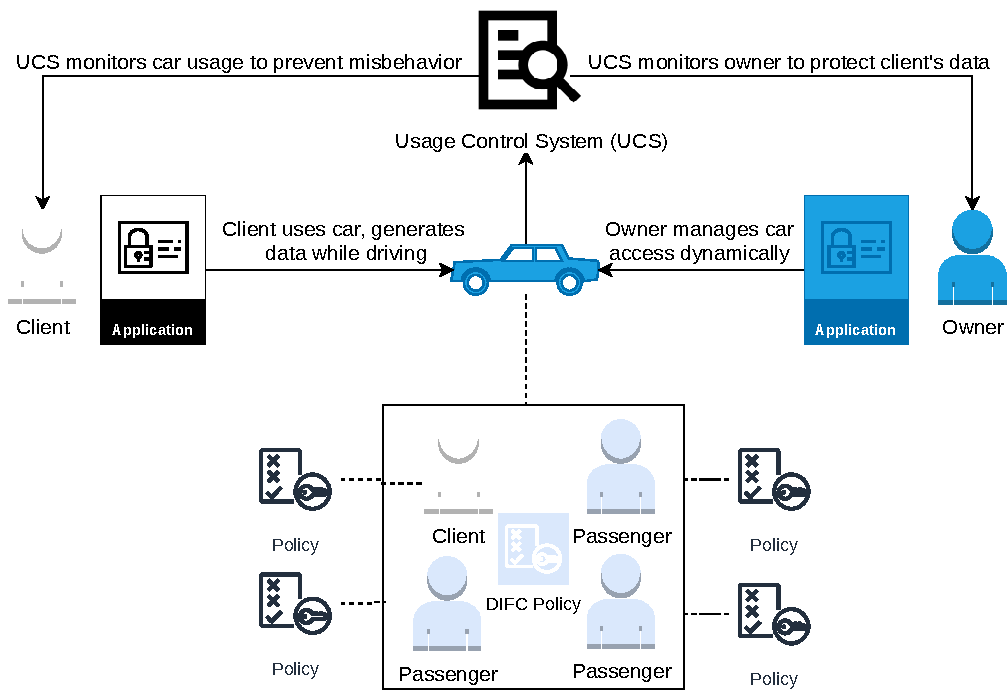
\includegraphics[width=\textwidth]{Images/framework_IFIP_alt.pdf}
\caption{Car sharing scenario and policies by car renter and occupants}
\label{F_DIFC_car_pooling}

\end{figure}
\subsection{Additional functions for DIFC and network status aspects}
\cul{As DIFC is only mentioned as an external specification in the state of the art}, DIFC objects, namely values, slots, channels and labels are not formalized in usage control models \emph{per se}. However, data $d \in \mathcal{D}$ can be regarded as DIFC values. Similarly, as containers hold the data, they can be considered as slots as defined in the DIFC specification \cul{and have labels attached to them}. A set of labels is noted $\mathcal{L}$, and can be composed of labels on any of the three DIFC objects that may be labeled, i.e., data, slots, and values. For convenience, we keep track of the objects associated with a label, such that $l.objects$ returns the list of data, slots or values associated with the label $l$. 

Having different labels, data and containers may have conflicting policies. Detecting conflicts is crucial to enforce information flow policies, as a decision must be taken to prioritize either the container labeling or the data labeling. Detecting the conflicts requires additional functions, to fetch the labels associated to containers and data, which are defined here as part of the contribution:
\begin{itemize}
    \item[] (1) \emph{labelC}: $\mathcal{P}(\mathcal{C}) \to \mathcal{P}(\mathcal{L})$. Given a set of containers, returns the labels associated with the containers: $\forall c \in \mathcal{C}$, \emph{labelC}$(c) \overset{def}{=} \{ l \in \mathcal{L} \ | c \in l.objects \} $; 
    \item[] (2) \emph{labelD}: $\mathcal{P}(\mathcal{D}) \to \mathcal{P}(\mathcal{L})$.
    Given a set of data, returns the labels associated with the data items: $ \forall d \in \mathcal{D}$, \emph{labelD}$(d) \overset{def}{=} \{ l \in \mathcal{L} \ | d \in l.objects \} $
    \item[] (3) \emph{conflict}: $\mathcal{P}(\mathcal{C}) \times \mathcal{P}(\mathcal{D}) \to \mathcal{P}(\mathcal{Y}) $. Given a set of containers $\mathcal{C}$ and data $\mathcal{D}$, returns the set of systems where there is a difference between the label associated with a container and the label of one of their known data. This function relies on \emph{knowD} (cf. Section \ref{ss_distributed_system_model}) to identify the containers $C$ knowing $d$ in the first place, then, by comparing the labels of all $c \in C$ with the labels of $d$ in $\mathcal{D}$:
    $ \forall c \in \mathcal{C}, \forall d \in \mathcal{D}
    $, \emph{conflict}$(c,d) \overset{def}{=} \{ y \in \mathcal{Y} | \exists (c,d) :$ \emph{labelC}$(c) \neq$ \emph{labelD}$(d) \}$;
\end{itemize}

The \emph{conflict} function, based on the \emph{labelC} and \emph{labelD} auxiliary functions, is dedicated to detecting individual systems $\mathcal{Y}$ where there is a conflict between the data label and the label of the container holding the data. These systems are of interest because this situation requires deciding which label should be prioritized, e.g., by considering the label representing the most restrictive policy.

\rul{In the car sharing scenario, a car owner $car_{own}$ is allowed to access the data container in its car $c_{car}$, but may not have access to the geolocation of the car $d_{GPS}$ stored in $c_{car}$. The car renter $car_{rent}$ or one of the car occupants $\mathcal{O}$ may apply labels to $d_{GPS}$ that may prevent the $car_{rent}$ from reading $d_{GPS}$. Detecting a conflict between the label $l_{c_{car}}$ applied to the container $c_{car}$ and the label $l_{d_{GPS}}$ applied to the data $d_{GPS}$ enables to block the dissemination to $car_{own}$. In that case, the security policy is to consider that the data label has priority over the container label. This policy is defined by the system administrator, and could be different, e.g., deny access in case of conflict is detected which would have the same result in this example.}

\textbf{Functions for network status.} Distributed systems are used in a diversity of networks, including the Internet of Things and peer-to-peer networks. These networks are inherently dynamic, with devices and peers connecting and disconnecting very frequently. Besides, the network may be intermittent or unreliable. For proper policy evaluation, it is consequently required to determine whether an individual system or a set of systems $\mathcal{Y}$ are currently connected to a system. \mul{More accurately, an individual (or a set of) system is considered disconnected if it can not be reached by the usage control system. The main concern in our case is the possibility to evaluate policies, and it avoids introducing more intricate notions, like relative disconnection between two individual systems}. By extension, it makes it possible to identify the subset of systems $\mathcal{Y}$ where a container $\mathcal{C}$ resides and that is connected to the distributed network. This leads to the definition of the following functions:

\begin{enumerate}
    \item[(1)] \emph{connected} : $\mathcal{Y} \times \mathbb{N} \times \prod \mathcal{T} \to \mathcal{P(Y)}$. Given a set of individual systems $\mathcal{Y}$, a point in time $i \in \mathbb{N}$ and a tuple of traces, return the subset of individual systems that are reachable in the network at this point in time. \mul{Traces are needed because the connection status depends on the timesteps considered}. An individual system is considered connected if there is no disconnection $e_{disconnect}$ in the traces, i.e., an event whose name $e$.name = disconnect. \emph{connected} is defined as: 
    \begin{center}
     $\forall y \in \mathcal{Y}, i \in \mathbb{N},  \tau \in \prod_{y \in \mathcal{Y}} \mathcal{T}_{y}$, \emph{connected}$(y,i,\tau)\overset{def}{=} \{ y \in \mathcal{Y} \ | \ \forall e \in  t_{y}^{\tau}(i), \ $e$.name \neq disconnect\}$  
    \end{center}

    \item[(2)] \emph{availableC} : $\mathcal{P(C) } \times \mathbb{N} \times \prod \mathcal{T} \to \mathcal{P(Y})  $. Given a set of containers, a point in time and a tuple of concurrently executing traces $\mathcal{T}$, \emph{availableC} returns the set of currently reachable systems in which one of the containers $c \in \mathcal{C}$ resides. The formal definition of \emph{availableC} is:
    \begin{center}
    $\forall C \in \mathcal{C}, i \in \mathbb{N},  \tau \in \prod_{y \in \mathcal{Y}} \mathcal{T}_{y}: \emph{availableC}(C) \overset{def}{=} \{y \in \mathcal{Y} \ | \ \mathcal{C}_{y} \cap C \neq \emptyset\ \wedge$ \emph{connected}$(y,i,\tau) \cap $\emph{knowC}$(C) \neq \emptyset\} $;
    \end{center}
    
    \item[(3)] \emph{availableD} : $\mathcal{P}(\mathcal{D}) \times \mathbb{N} \times \prod \mathcal{T} \to \mathcal{P}(\mathcal{Y})$. Given a set of data items $\mathcal{D}$, a point in time $ t \in \mathbb{N}$ and a tuple of concurrently executing traces $\mathcal{T}$, \emph{availableD} returns the set of currently reachable systems where one or more containers are storing at least one of the data items $d \in \mathcal{D}$. \emph{availableD} is formally defined as follows:
    \begin{center}
      $\forall D \subseteq \mathcal{D}, i \in \mathbb{N}, \tau \in \prod_{y \in \mathcal{Y}} \mathcal{T}_{y}: $ \emph{availableD}$(D,i,\tau) \overset{def}{=} \{y \in \mathcal{Y} \ | \ \exists c \in \mathcal{C}_{y}, t_{y}^{\tau} \in \mathcal{T}_{y}, \sigma_{t_{y}^{\tau}}^{i} \in \Sigma_{y}: D  \cap \sigma_{t_{y}^{\tau}}^{i}.s(c)  \neq \emptyset \ \wedge$ \emph{connected}$(y,i,\tau) \cap$\emph{knowD}$(D,i,\tau) \neq \emptyset \}$
     \end{center}
\end{enumerate}

\rul{As the cars are moving objects, the need to manage connection status is paramount in the car sharing scenario. First, a car may be disconnected temporarily from the network, e.g., driving through a tunnel, which is detected by the \emph{connected} function. As a consequence, if the location of the car $d_{GPS}$ is stored only in the car \emph{via} a data container $c_{car}$ in the car, it becomes unavailable to the car owner $car_{own}$, who should be notified. This is reflected by both \emph{availableC} and \emph{availableD}, for respectively the container $c_{car}$ and the data $d_{GPS}$.}

\sul{In this section, we introduced several formal functions to handle DIFC labels (\emph{labelC} and \emph{labelD}) and detect conflicts between the data and their containers (\emph{conflict}). Additionally, we introduced functions to handle the status of the network, detecting if a set of individual systems is connected or not (\emph{connected}), and consequently if a container can be accessed and data fetched depending on the system's state. In the next section, we introduce the new components needed in the usage control system architecture to handle DIFC aspects, as part of our contribution.}

\subsection{Integrating DIFC components in the usage control system}
\label{ss_architectural_integration_of_difc}
Distributing the system requires the introduction of several components for the UCS to handle cross-system communication, information flow tracking and policy deployment. In addition to the existing UCS components in centralized settings (cf. Section \ref{ss_ucon_architecture}), the usage control system has the following components:
\begin{itemize}
    \item The \emph{Distribution Management Point} (DMP) organizes the information flow between systems and the policy propagation while relying on a distributed database to coordinate the policy decisions,
  \item the \emph{PDP server} provides the interface so that PEPs can request data usage control decisions.
 \item The \emph{PIP Server} provides the interface to fetch environment attributes from the PIPs.
  \item The \emph{DMP Server} allows communication with remote DMPs. 
 \item the \emph{Context Handler} orders and processes requests sent to the servers, 
notably to avoid event reordering and race conditions. The architecture is represented in Figure \ref{F_Kelbert_architecture_DIFC_enhanced};
\item The \emph{communication manager} manages all external communication 
and runs servers to show the components' functionalities to the outside. It is not a component itself and is composed of the Context Handler, PDP server, PIP server and DMP server. 
\end{itemize}
% Distributing the system requires the introduction of several components for the UCS to handle cross-system communication, information flow tracking and policy deployment. The \emph{Distribution Management Point} (DMP) organizes the information flow between systems and the policy propagation while relying on a distributed database to coordinate the policy decisions.
%  The \emph{communication manager} (included in the controller) manages all external communication 
% and runs servers to show the components' functionalities to the outside. In particular, the \emph{PDP server} provides the interface so that PEPs can request data usage control decisions.
% The \emph{PIP Server} provides the interface to fetch environment attributes from the PIPs. The \emph{DMP Server} allows communication with remote DMPs. Finally, the \emph{Context Handler} orders and processes requests sent to the servers, 
% notably to avoid event reordering and race conditions. The architecture is represented in Figure \ref{F_Kelbert_architecture_DIFC_enhanced}. 



\textbf{Additional components for DIFC processing.} Decentralized information flow control is often processed using a dedicated instance, called the DIFC platform \cite{Schultz2013} or DIFC center \cite{Lu2022}. There are different ways to process DIFC tasks: either use already existing components, e.g., the PDP, or introduce new dedicated components to manage DIFC aspects. Since DIFC policies differ from usage control policies, it is better to introduce dedicated components to handle DIFC aspects.

For distribution purposes, DIFC platform components are added as a novelty to the existing architecture \cite{Lu2022}, and interact only with the DMP to distribute the policies to other individual systems $\mathcal{Y}$ or system set $Y$. The DIFC platform is responsible for pre-processing (DPP), privilege extraction (PP) and data labeling (DLP). Each operation has a dedicated component, as depicted in Figure~\ref{F_Kelbert_architecture_DIFC_enhanced}:
\begin{itemize}
    \item the \emph{Data Labeling Point} (DLP) is responsible for labeling data, slots and channels;
    \item the \emph{Privilege Point} (PP) is responsible for privilege extraction, converting labels into actual access rights;
    \item the \emph{Data Pre-processing Point} (DPP) routes the data to other components of the DIFC platform. If the data is unlabeled, the data are sent to the DLP. Conversely, labeled data are sent to PP for privilege extraction (cf. Section \ref{ss_DIFC_model}).
\end{itemize}


\textbf{Existing interfaces.}
Interfaces are associated with the components to provide several methods for usage control.
The PDP server provides two interfaces \texttt{IPmp2Pdp} and \texttt{IPep2Pdp}, providing methods to deploy or retrieve policies,  
to signal system events and to await policy decisions.
The PDP uses interface \texttt{IPdp2Pip} to evaluate state-based operators, retrieve all data stored in a  
container $\mathcal{C}$, and signal system events associated with information flow. The PMP uses interface \texttt{IPmp2Pip} to inform the PIP about initial data
representations. Interface \texttt{IDmp2Pip} is used by the DMP if there are cross-system data flows.
The DMP provides interface \texttt{IDmp2Pmp}, which is used by the local DMP to deploy policies and to retrieve currently
deployed policies. The DMP additionally provides four interfaces:

\begin{enumerate}
    \item \texttt{IPip2Dmp} allows the PIP to inform the DMP about data flows to the remote socket
    containers;
    \item \texttt{IPdp2Dmp} enables the coordination of policy decisions across PDPs. This includes methods to notify
    that an operator’s state has changed, to query whether the state of some operator has changed at remote PDPs, and
    to synchronize the points in time in which policies are evaluated;
    \item \texttt{IPmp2Dmp} allows the PMP to register policies at
    the DMP;
    \item \texttt{IDmp2Dmp} provides functionalities for cross-system information flow tracking and policy propagation between
    remote DMPs.
\end{enumerate}

% \textbf{DIFC components.} Similarly, the introduction of DIFC requires specific components to do the following tasks:

% \begin{itemize}
%     \item labeling (including slots and channels);
%     \item privilege extraction, i.e., conversion of the labels into actual access rights;
%     \item data processing, such as declassifications or restrictions (cf. Section \ref{ss_DIFC_model}).
% \end{itemize}

% \begin{figure}[t]
% \centering
%  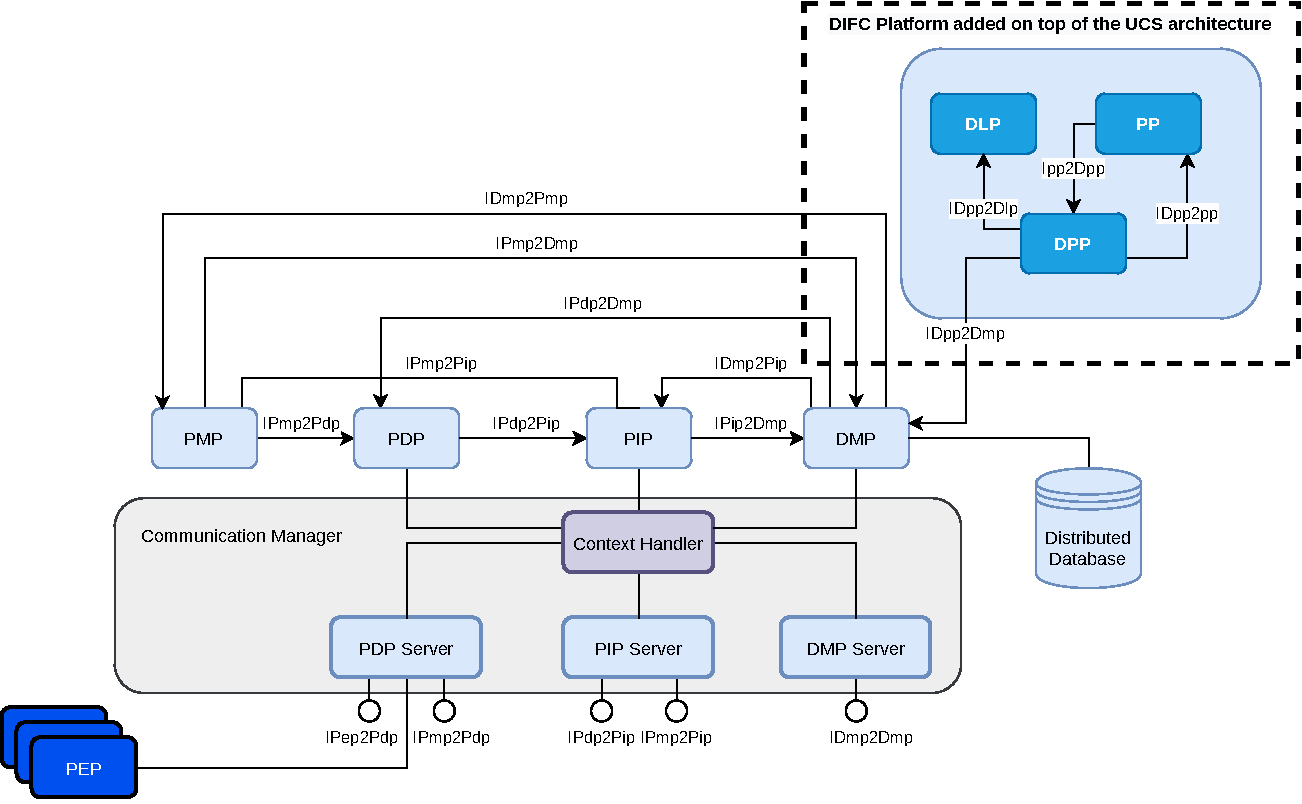
\includegraphics[width=\columnwidth]{Images/Kelbert_architecture_DIFC_enhanced.pdf}
% \caption{Architecture of the usage control system \cite{Kelbert2018}, with the DIFC platform for policy labeling as a contribution.}
% \label{F_Kelbert_architecture_DIFC_enhanced}

% \end{figure}
% This processing is often provided by a dedicated instance, called the DIFC platform \cite{Lu2022} or DIFC platform \cite{Schultz2013}. There are different ways to fulfill these tasks: either use already existing components, e.g., the PDP, or introduce new dedicated components to manage DIFC aspects. Since DIFC policies differ from usage control policies, it is better to introduce dedicated components to handle DIFC aspects.

% For distribution purposes, DIFC platform components are added as a novelty to the existing architecture, and interact only with the DMP to distribute the policies to other individual systems $\mathcal{Y}$ or system set $Y$. The DIFC platform is responsible for pre-processing (DPre), privilege extraction (PP) and data labeling (LD). Each operation has a dedicated component, as depicted in Figure~\ref{F_Kelbert_architecture_DIFC_enhanced}.

 \begin{figure}[t]
 \centering
 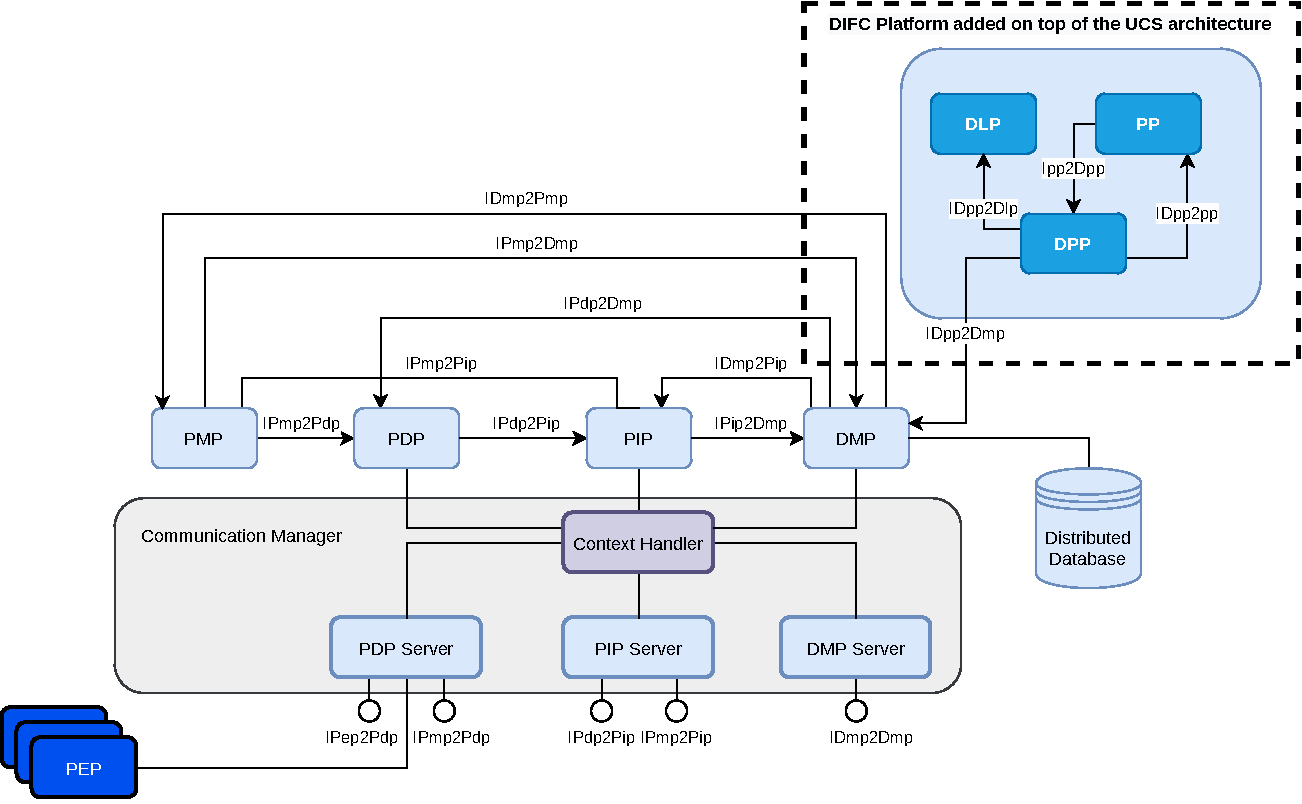
\includegraphics[width=\columnwidth]{Images/Kelbert_architecture_DIFC_enhanced.pdf}
 \caption{Architecture of the usage control system \cite{Kelbert2018}, with the DIFC platform for policy labeling as a contribution.}
\label{F_Kelbert_architecture_DIFC_enhanced}
\end{figure}

\textbf{DIFC interfaces.} As part of the contribution, the introduction of DIFC components requires to add four new interfaces (represented in Figure \ref{F_Kelbert_architecture_DIFC_enhanced}):
\begin{enumerate}
    \item \texttt{IDPP2DLP} is an interface implemented so that the data can be labeled by the data labeling point (DLP) if the component DPre detects that it has not been labeled yet;
    \item \texttt{IPP2DPP} is needed to answer a request from the data processing point (DPP) and to notify it with updates of privileges;
    \item \texttt{IDPP2PP} is an interface that enables the data pre-processing point (DPP) to fetch the required privileges from the dedicated privilege point; 
    \item \texttt{IDPP2DMP} provide methods so that the DIFC policies are propagated to all individual systems.
\end{enumerate}
%\section{Model checking}
%\label{S_model_checking}

%To ensure the correctness of the proposed system's design, we rely on model checking using \emph{TLC}, introduced in Section \ref{ss_background_tla}. Model checking is used in formal verification for early detection of errors or potential issues in a system design or specification, for an exhaustive exploration of all system states and behaviors and for design validation. The validation of the proposed function \emph{connected} is detailed in Section \ref{ss_validation}.

%\subsection{Background on TLA+ and TLC}
%\label{ss_background_tla}
%TLA+ is a general-purpose formal specification language based on
%the \emph{Temporal Logic of Actions} for specifying real-time properties
%\cite{Lamport1992}. It is designed for modeling and reasoning on concurrent and 
%distributed systems, which makes it appropriate to check our proposed model.

%\textbf{TLA+ model checker.} The TLA+ specifications corresponding to the proposed model's functions can be checked using model checking tools such as TLC (TLA+ Model Checker) or formally proven using theorem provers like TLAPS (TLA+ Proof System).

%\subsection{Validation of Connected function.}
%\label{ss_validation}

%\nathanael{Décrire ce qui est fait dans le code TLA+ pour l'exemple}
%\begin{figure}[t]
%    \centering
%     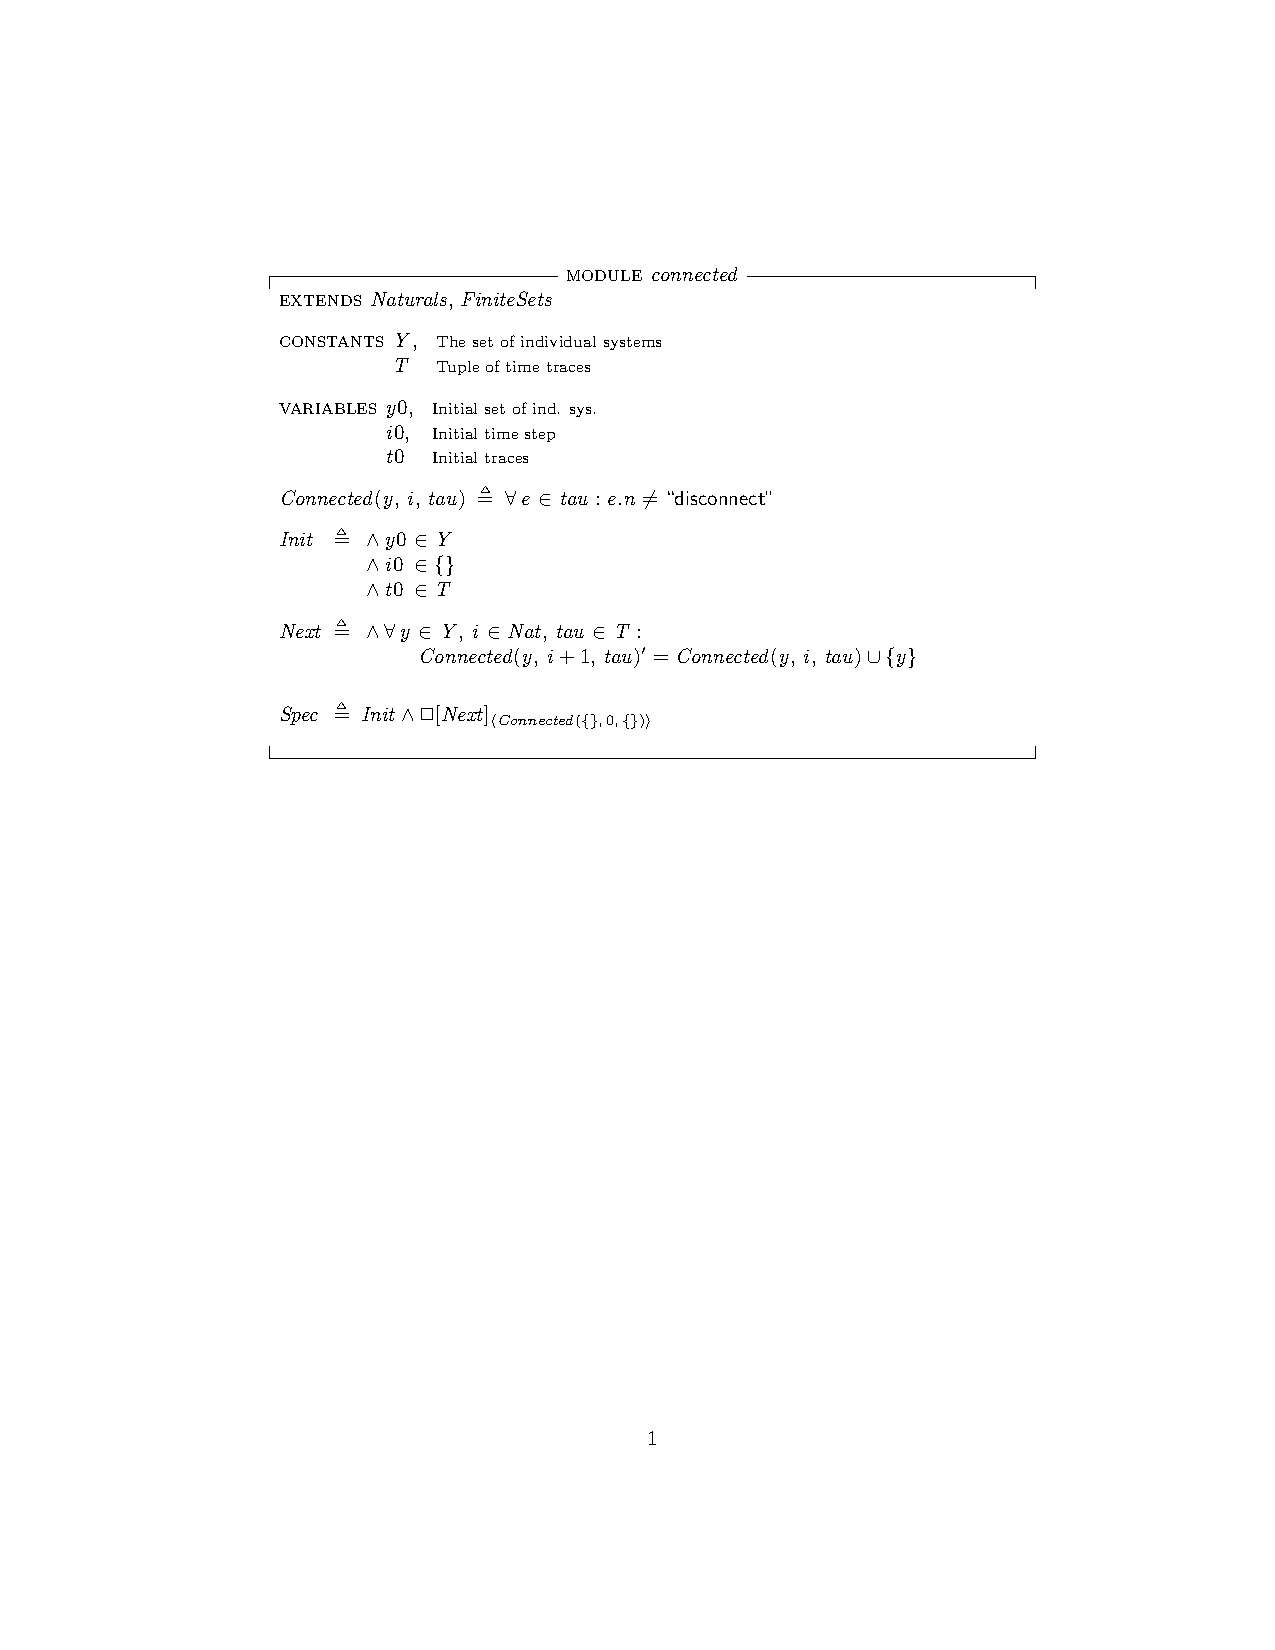
\includegraphics[trim=4.25cm 15cm 4cm 4cm, clip=true, width=\textwidth]{Images/connected.pdf}
%    \caption{Specification of connected function in TLA+}
%    \label{F_connected_TLA+}
%    \end{figure}
 
%\subsection{Validation of Conflict function.}

\section{Conclusion}
\label{S_conclusion_formalism}

In this chapter, we propose an extended usage control model for distributed systems, 
by introducing elements of decentralized information flow control (DIFC) into the state-of-the-art formalism~\cite{Kelbert2018}. 
The extension of the former modeling is justified by the need to consider all the aspects of the distribution, including 
the user-side policy definition, as well as specificities of IoT networks that require a more sophisticated 
distributed system modeling. Recent advances in DIFC, based on evolving coding practices \cite{Liu2022}, make DIFC usable 
and justify its consideration in distributed system modeling.
Although this formalism enables the addition of external specification, using the dedicated \underline{evalExt} operator, 
we state that DIFC actually requires dedicated components and functions. As a consequence, we extend the existing usage control architecture 
adding a privilege point (PP), a data pre-processing component (DPre) and a last component dedicated to data labeling (DL). Interfaces 
are also considered to enable cross-component communication. Additionally, 
we define new functions to identify the relevant parts of the distributed system. The main function considered, \emph{conflict},
detects individual systems $\mathcal{Y}$ (cf. Section \ref{ss_distributed_system_model}) of the distributed system where the
security policy on the data and their storage location are conflicting.



\newpage \ \newpage
%----------------------------------------------------------------------
\chapter{Conclusion and Future Works}
\label{C_conclusion}
\minitoc


This concluding chapter first summarizes the contributions of this thesis (Section \ref{S_summary}), before introducing the limitations of the presented works, notably concerning the key technologies used 
in the different contributions (Section \ref{S_limits}). Finally, different research directions are provided, either to improve the existing work or to extend the contributions to solve other research issues (Section \ref{S_future_works}). 

\section{Summary}
\label{S_summary}

Throughout this document, we proposed several contributions that addressed four different research objectives. These objectives fall within the general topic of privacy preservation, security and performance 
in the Internet of Things, which are paramount for the nearing massive adoption of IoT devices. The contributions of this thesis can be summarized as follows. 
A key aspect regarding these contributions is that they addressed these requirements altogether, i.e., performance, privacy and security simultaneously. Besides,
both practical aspects, such as integration with performance tests (Section \ref{S_performance_evaluation}) and theoretical, formal ones (Chapter \ref{C_formalism})
were presented in this work. These contributions are summarized as follows.

\textbf{Framework for performance, privacy and security in the Internet of Things.} (\hyperref[obj:1]{\emph{Objective 1}}, \hyperref[obj:23]{\emph{Objective 2}}). 
This first contribution is the design of a framework whose purpose is to address the privacy, security and
performance requirements of the Internet of Things. The basis of the framework is the IOTA technology. The framework is centralized around the IOTA technology, used for its zero-fee transactions and 
attractive metrics for the Internet of Things. Other components are also related to IOTA, such as IOTA Access to monitor physical access to the Internet of Things devices, such as cars or doors. A decentralized mixer 
to obfuscate IOTA transactions is also part of the framework, as defined by Sarfraz \cite{Sarfraz2019}. Mixing was complemented with merge avoidance, to further improve the privacy of the users. Finally, usage control mechanisms are introduced so that users can monitor the use and dissemination of their data,
by defining policies.

\textbf{Integration of usage control with distributed ledgers.} (\hyperref[obj:23]{\emph{Objective 3}}).
This contribution proposes to integrate usage control with distributed ledgers based on directed acyclic graphs (DAG), after an analysis of suitable distributed ledger technologies. Private blockchains (or DAGs) are also suitable, 
but have limited scalability due to centralized governance, and were not selected for the experiments. The benefits of integration are to make both 
the usage control system and the distributed ledger work in synergy: 1) the components of the usage control system contribute
to the network security, by verifying the state of the ledger as a DAG node; 2) the usage control system processes the transaction data without intermediaries,
which is faster and more reliable. 
An implementation of usage control integration is proposed on IOTA. Performance tests are conducted on this implementation, showing approximately a 90\% decrease
of the time needed to push transactions and make an access decision when the UCS is integrated.

\textbf{Data usage control model for distributed systems.} (\hyperref[obj:4]{\emph{Objective 4}}). In the last contribution, we proposed an extended model for data usage 
control in distributed systems. The need to define an all-encompassing model for distributed systems is motivated by their use in Internet of Things networks. To improve the existing model, we added dedicated functions
and components dedicated to \emph{decentralized information flow control}. This enables users to define policies jointly, 
removing the need for a centralized entity responsible for policy management. Decentralized information flow control 
has seen recent improvements, notably because of current coding practices \cite{Liu2022}, which justifies its 
introduction as a relevant, usable tool in distributed systems. The model is also complemented by 
new functions considering the state of the individual entities of the network, as IoT networks 
can be unreliable, intermittent, and subject to frequent connections and disconnections.

\section{Limitations}
\label{S_limits}
There are several limitations in the thesis work that we discuss next, inherent to the technologies as part of the solutions such as IOTA, or due to validation aspects that could increase the confidence in the proposed solutions.

\textbf{Limitations of IOTA.}
IOTA is a key technology used in this thesis as a basis to address the research objectives, notably \hyperref[obj:1]{\emph{Objective 1}} (privacy-preserving zero-fee transactions), \hyperref[obj:23]{\emph{Objective 2}} (suitable distributed ledger for the IoT) and to a lesser extent \hyperref[obj:23]{\emph{Objective 3}} as DAG-based distributed ledger, including IOTA, are particularly fitted for integration (cf. Chapter \ref{C_integration}).
The main benefits of using IOTA are to benefit from the properties provided by DAG-based distributed ledgers, including:
\begin{enumerate}
    \item zero-fee transactions with the removal of the miner, or fundamentally, by trading a financial incentive with a cost-saving incentive;
    \item attractive metrics for IoT use cases, such as high transaction throughput;
    \item involvement of resource-constrained IoT devices.
\end{enumerate}

Yet, these claims are partly inaccurate in the first version of IOTA. While transactions are actually zero-fee, current performance metrics are limited compared to the expected metrics. In theory, the more transactions in the network, the faster transactions are confirmed, but more transactions also create congestion. This impacts negatively the confirmation rate and confirmation time \cite{Dong2019}. The phenomenon is due to the coordinator, the central component in charge of validating transactions during the early stages of IOTA. The second version of IOTA 2.0 (Coordicide \cite{Popov2020}) is designed to remove this component which should provide the expected network metrics in IOTA. Yet, it is not possible to anticipate accurately the release of IOTA 2.0.

Besides, the reliance of IOTA on a non-financial incentive could be troublesome in the future, as the IOTA network requires stable, full nodes to be reliable, while full nodes are expensive to run \cite{Dong2019}. The lack 
of motivation may hinder the network's ability to properly grow in the future, which is required to achieve the claimed high throughput.

\textbf{Evaluating the scalability of distributed ledgers.} Scalability has been identified as a key metric throughout this thesis work (cf. Section \ref{ss_performance_metrics}). Scalability is one of the expected benefits of decentralization, which was identified as 
one of the two criteria of interest to determine integrability (cf. \ref{ss_integrability_criteria}). Nevertheless, as discussed in Section \ref{ss_performance_metrics}, scalability is complex to define in the first place, and requires handling any possible bottleneck. 
Dong \emph{et al.} \cite{Dong2019} have proposed to evaluate scalability as "the changes in throughput and latency
when increasing the number of nodes", using the \emph{confirmation rate}. The confirmation rate measures the number of transactions confirmed\footnote{\cul{A transaction is confirmed if it is referenced by a milestone from the coordinator in IOTA (1.0).}} in a second, which is related to both throughput and latency. The results of \cul{Dong \emph{et al.}'s} evaluation show that the confirmation 
rate is at most 0.8tx.$s^{-1}$, much lower than IOTA's throughput. The Coordinator node of IOTA(1.0) is still a major obstacle to scalability considering the confirmation rate.

\textbf{Adoption of usage control.} If IOTA is the main technology used to answer IoT requirements in terms of performance, usage control is its counterpart concerning privacy needs in this thesis work. 
While it is a multipurpose technology with regard to the mitigation of privacy threats (cf. Section \ref{ss_mitigation}), it has several limitations preventing its adoption:

\begin{itemize}
    \item the complexity of implementing and managing UCON policies. UCON systems require detailed specification and configuration of access control rules, obligations, and conditions, which can be challenging to design and maintain, especially in large and dynamic systems. Additionally, UCON may face resistance or challenges in adoption due to compatibility issues with existing access control mechanisms and the need for integration with different components and platforms within an organization's infrastructure;
    \item the policy enforcement points are distributed on the monitored devices, which creates risks to the security and privacy of users. While these risks are usually mitigated using a trusted execution environment, this solution has shortcomings as the TEE itself may not be secured;
    \item the potential impact on system performance. Usage control systems involve additional computational overhead to evaluate and enforce access control policies at runtime, which may be limiting in several use cases. 
\end{itemize}


\section{Future works}
\label{S_future_works}
In this section, different prospects following this thesis work are developed. First, different works that could complete the proposed contribution are proposed. Additionally, orthogonal research topics are mentioned, that were not directly addressed in this work but which could benefit from its findings.
 
\subsection{Automatic generation of XACML policies for testing}
The contributions of this thesis often required to evaluate usage control policies, written in the XACML language. For instance, we assessed the 
time needed to evaluate an XACML policy in Chapter \ref{C_integration}, which is actually lightweight compared to other system and network calls.
However, defining XACML policies is a cumbersome process, which hinders the adoption of usage control in practice. First, the clear and exhaustive  
definition of the policies themselves can be difficult, including for testing purposes.
Besides, the translation from high-level policies to XACML policies is also tedious to do by hand (cf. Listing \ref{listing:XACML_policy}).
 
Several works in the literature have been developing tools to make the generation of XACML policies more user-friendly. Bertolino \emph{et al.} have proposed two different ways 
to derive XACML requests automatically for policy testing \cite{Bertolino2012}. The authors also underline the impossibility of manual specification of a set of test cases in XACML testing. 
Similarly, Xu \emph{et al.} use \emph{mutation-based tests} where access requests are derived from an original policy \cite{Xu2020}. While the same methodology was used in the presented thesis, the derivation was very basic and consisted 
of value substitution. Future works may include tests based on rigorous policy derivation.

% \textbf{Usable privacy.} Usable privacy by making usage control more user-friendly, e.g., with high-level understandable definitions or user-friendly interfaces, is poorly addressed by the literature. However,
% the literature has proposed several XACML policy editors such as UMU-XACML or ALFA \cite{Nergaard2015} to enable manual policy definitions without 
% writing policies from scratch in the XML language.


\subsection{Model checking on usage control model} 
For the \emph{Contribution 3}, we proposed an extension of the state-of-the-art usage control model in distributed systems. However, the model can have flaws in its definition, including the existing model we used as a basis. Model-checking tools exist to ensure the model's validity.

 TLA+ is a formal specification language developed by Leslie Lamport. It is used for designing, modeling, documentation, and verification of programs, especially concurrent systems and distributed systems \cite{Lamport1992}. TLC is a model checker designed for TLA+ that can be used to detect errors in TLA+ specifications.
 The validation of the model could be of interest in particular when using the model in well-defined use cases. Besides, some functions such as the \emph{conflict} function, responsible for detecting collisions between the labels of data and their containers, might have side effects and not be doable in practice, e.g., due to communication costs. An implementation with performance testing could exclude this risk and would fit the research objective (\hyperref[obj:56]{\emph{Objective 6}}) regarding validation using a proof of concept. 
 
\subsection{IOTA-based privacy-preserving machine learning}
 The Internet of Things can leverage advanced machine learning algorithms for its applications \cite{Ali2021}. Machine learning (ML) and deep learning (DL) algorithms have significantly been improved and used in diverse applications, including computer vision, natural language processing and automated speech recognition. Several Internet of Things systems, such as autonomous vehicles, UAVs, drones or security robots, heavily rely on ML/DL-based technologies \cite{Jiang2022}. However, considering the huge quantity of data stored at a central cloud server, adopting centralized machine learning algorithms is not a viable option due to computation cost and privacy leakage issues. Yet, leveraging distributed data for application purposes is still a challenging task \cite{Ali2021}. To address this challenge, \emph{federated learning} (FL) is a promising solution that distributes learning to the end devices without sharing personal data with the central server. In federated learning, the central server only orchestrates the learning process, and only the updates of model parameters are shared between end devices and the central orchestrator. Therefore, the central server does not need access to actual data to learn, reducing privacy risks.
 
 \textbf{Blockchain-based federated learning.} Federated learning being distributed by nature, blockchain-enabled federated learning has been gathering significant attention, which is shown by frequent and recent surveys \cite{Lee2021, Issa2023, Qu2023} or systematic literature reviews \cite{Dongkun2021, Qammar2023}. Blockchains are leveraged in federated learning for the following reasons:
 
 \begin{itemize}
     \item \emph{smart contracts} can be used to coordinate federated learning. Smart contracts can validate node contributions, compute the global model automatically, record the performance of nodes on the ledger and provide incentives to nodes based on performance \cite{Issa2023};
     \item improving security and privacy by removing the \rul{need for a} central server \cite{Issa2023}, mitigating the \emph{single point of failure} threat. \rul{The global model can be aggregated by delegates from the local models, then, put on the distributed ledger. In return, nodes can download the global model and use it to train their local models} \cite{Yunlong2020};
     \item enhanced auditability and accountability of the nodes \cite{Issa2023}.
 \end{itemize}
 
 Yet, federated learning using blockchains still has to address several challenges to preserve privacy and to handle the Internet of Things constraints, e.g., low computation and storage capabilities \cite{Issa2023}. These challenges are very similar to what has been addressed in Chapter \ref{C_solving_trilemma} and Chapter \ref{C_integration}) and
 most of the research objectives of this paper (\hyperref[obj:23]{\emph{Objective 2}}, and indirectly \hyperref[obj:23]{\emph{Objective 3}}) but integrating federated learning instead of usage control). The results of this thesis work could also be extended to federated learning.
 
 \textbf{IOTA-based federated learning.} Distributed ledgers based on DAGs are not mentioned in the literature as a potential solution outperforming blockchains for federated learning \cite{Issa2023, Qu2023}. To my knowledge, only one research article from Lu \emph{et al.} \cite{Yunlong2020} suggests the use of a DAG-based distributed ledger combined with a private blockchain for secure data sharing and
 federated learning. \rul{The private blockchain is used for the global aggregation of the models and the DAG is responsible for asynchronous local training.} In the authors' setting, both the DAG and the blockchain are permissioned, which prevents its adoption in large-scale networks. IOTA could be leveraged as it can incorporate Internet of Things devices into its network efficiently, which is not the case of blockchains in general (cf. Section \ref{S_distributed_ledgers}).

\subsection{IOTA for supporting Self-Sovereign Identities}
\label{ss_ssi}
 
\cul{Self-Sovereign Identity (SSI) is an approach in which subjects
are in full control of their own digital identities} \cite{Fedrecheski2020}. 
\cul{SSI contrasts with current digital
identity solutions that are centralized which creates privacy and security issues} \cite{Fedrecheski2020}.

\cul{Self-Sovereign Identities have several benefits to the Internet of Things. In particular, SSIs are \emph{owner-centric} and enable users to be the root of trust of their devices instead of a third party. The identities of users and their devices are stored locally on their own devices and are disclosed selectively by the users themselves, improving privacy in contrast with centralized identity management. Removing the need for a third party to manage identities increases the decentralization in the network and removes a single point of failure from the network} \cite{Fedrecheski2020}. 

\cul{Yet, the adoption of the SSI paradigm in IoT networks faces several hurdles, both technical and non-technical e.g., standardization} \cite{Fedrecheski2020}. \cul{The technical aspects include the limitations of \emph{constrained devices}. To implement Self-Sovereign Identities, the devices must be able to run asymmetric cryptography and handle the communication overhead}.
%     \item \emph{traceability}: global tracking should be avoided and is often not possible without a central authority;
% \end{itemize}

\cul{The IOTA technology, due to its ability to integrate constrained devices into its consensus and its network, is a promising technology to address the first technical limit. In particular, IOTA gives the possibility to deploy nodes to the users, to which the computation-intensive aspects can be delegated. Existing works have proposed to use IOTA as the basis of a SSI system for the Internet of Things devices} \cite{Gebresilassie2020} \cul{and IOTA itself has a module to generate decentralized identities} \cite{IOTA2020}. Gebresilassie \emph{et al.} propose to use DAGs as building blocks for a DAG node identity management system, in particular to manage node reputation. However, the contribution remains very elusive on many key technical aspects such as conditions for enrolling nodes in the SSI system, desired security properties, transaction content and security analysis which still leaves many unknowns before a possible implementation within a proof of concept. 


% \bibliographystyle{plain}
%  \bibliographystyle{alpha-fr}
\bibliographystyle{apalike}
\bibliography{bib/bibliography,bib/blockchain,bib/privacy,bib/iot,bib/formalism} 



%------------------------------------------------!-------------------------------

\appendix

\chapter{Glossary}
\label{A_glossary}
\begin{itemize}
    \item[] \textbf{DApp}: DApps are open-source, decentralized applications that can operate autonomously and without human intervention. DApps make use of cryptocurrencies or tokens, are executed in a network of computers and store outputs in public ledgers \cite{Andoni2018};
    \item[] \textbf{DIFC}: Decentralized information flow control (DIFC) allows users to control the flow of their
    information without imposing the rigid constraints of a traditional
    multilevel security system \cite{Myers1997}; 
    \item[] \textbf{DLT}: Distributed Ledger Technology. A distributed ledger is a register containing a set of transactions.
    This ledger instead of being stored in a single place, the central
    server, is duplicated on a set of machines. The fact that the
    ledger is copied identically multiple times makes it expensive
    to modify it: it requires to be changed on every node of the network. \cite{Quiniou2019};
    \item[] \textbf{DPoS}: Delegated Proof of Stake (DPoS) is a variant of PoS in which "all the stakeholders vote to choose some nodes as witnesses and delegates. Witnesses are responsible and rewarded for creating new blocks. The delegates are responsible for maintaining the network
    and proposing changes such as block sizes, transaction fees, or reward amount" \cite{Salimitari2020};
    \item[] \textbf{Hashgraph}: Hedera Hashgraph is a distributed ledger technology that has a new form of distributed consensus \cite{Baird2018}. It provides fast and ordered transactions, as well as secure infrastructure to run decentralized applications; 
    \item[] \textbf{IFC}: Information Flow Control (IFC) \cite{Denning1976} is 
    "a concept requiring that information
    transfers within a system be controlled so that information in
    certain types of objects cannot, via any channel within the
    system, flow to certain other types of objects" \cite{rfc4949}  ;
    \item[] \textbf{IIoT}: Industrial Internet of Things, refers to the use of IoT technologies in the manufacturing industry \cite{Boyes2018};
    \item[] \textbf{IoT}: Internet of Things, the ever-growing network of physical objects that feature an IP address for internet connectivity, and the communication that occurs between these objects and other Internet-enabled devices and systems \cite{Berte2018}. It is to be noted that the Internet of Things has manifold definitions \cite{Atzori2010}; 
    \item[] \textbf{IOTA}: IOTA is a cryptocurrency for the Internet-of-Things (IoT) industry. The main feature of this
    novel cryptocurrency is the tangle, a directed acyclic graph (DAG) for storing transactions. It offers features that are required to establish a machine-
    to-machine micropayment system \cite{Popov2017}.
    \item[] \textbf{GDPR}: European \emph{General Data Protection Regulation} \cite{EUdataregulations2018};
    \item[] \textbf{Metadata}: Metadata is structured information that describes, explains, locates, or otherwise makes it
    easier to retrieve, use, or manage
    an information resource. Metadata
    is often called data about data or 
    information about information \cite{NISO2004};
    \item[] \textbf{PoA}: The proof of authority (PoA) is a consensus algorithm used most of the
    time for private blockchains. It makes it possible to designate
    nodes of the network as validators, these nodes having the role
    of determining the state of the ledger for the entire network \cite{Quiniou2019}. It significantly increases the speed of
    transaction validations, even if centralization is increased \cite{Quiniou2019};
    \item[] \textbf{PBFT}: In Practical byzantine fault tolerance (PBFT), all the nodes should participate in the voting process in order to add the next block and the consensus
    is reached when more than two-thirds of all nodes agree upon that block. PBFT can tolerate malicious behavior from up to
    one-third of all nodes to perform normally \cite{Salimitari2020};
    \item[] \textbf{PoET}: Proof of elapsed time (PoET) is a consensus method proposed by Intel that works similarly to PoW but with significantly lower
    energy consumption. In this method, miners have to solve a hash problem similar to that of PoW. However, instead of a
    competition between miners to solve the next block, the winning miner is randomly chosen based on a random wait time.
    The winning miner is the one whose timer expires first \cite{Salimitari2020};
    \item[] \textbf{PoS}: the proof of stake (PoS) is an alternative consensus algorithm to the
    proof of work which provides the right to create the next block
    to an active validator on the network that has deposited units
    of the cryptocurrency of this blockchain. The proof of stake is less energy intensive than proof of work \cite{Quiniou2019};
    \item[] \textbf{PoW}: Proof of Work is a computation race taking the form of a cryptographic puzzle, used by the Bitcoin cryptocurrency to elect the node responsible for writing the next transaction on the ledger \cite{Nakamoto2008}; 
    \item[] \textbf{TEE}: a Trusted Execution Environment (TEE) is a tamper-resistant processing environment that runs on a separation
    kernel. It guarantees the authenticity of the executed code, the
    integrity of the runtime states (e.g. CPU registers, memory
    and sensitive I/O), and the confidentiality of its code, data
    and runtime states stored on a persistent memory \cite{Sabt2015};
    \item[] \textbf{UCON} is a model for data access control that allows for dynamic decision-making based on attributes such as context, time, and user behavior \cite{Park2004};
    \item[] \textbf{UCS}: Usage Control System, an entity responsible for monitoring the data usage and dissemination, according to user-defined policies;
    \item[] \textbf{XACML}: The eXtensible Access Control Markup Language (XACML) is an XML-based standard markup language for specifying access control policies. The standard, published by OASIS, defines a declarative fine-grained, attribute-based access control policy language, an architecture, and a processing model describing how to evaluate access requests according to the rules defined in policies \cite{Axiomatics2023}.
\end{itemize}

\chapter{Publications}
\label{A_Publications}
\section*{Conferences and journals}

\begin{itemize}
    \item[] N. Denis, M. Laurent and S. Chabridon, \emph{Integrating Usage Control into Distributed Ledger Technology for Internet of Things Privacy} in IEEE Internet of Things Journal, \url{https://doi.org/10.1109/JIOT.2023.3283300}, June 2023;
    \item[] N. Denis, S. Chabridon, M. Laurent, \emph{Bringing Privacy, Security and Performance to the Internet of Things through Usage Control and Blockchains},  IFIP Summer School on Privacy and Identity Management 2021, IFIP Advanced in Information and Communication Technologies Series (Eds. I. Schiering, M. Friedewald, S. Krenn, S. Schiffner), \url{https://doi.org/10.1007/978-3-030-99100-5_6}, March 2022.
\end{itemize}

\section*{Submission}

\begin{itemize}
    \item N. Denis,  S. Chabridon, M. Laurent, \emph{Bringing Privacy, Security and Performance to the Internet of Things using IOTA and Usage Control} in Annals of Telecommunications (extended paper), June 2023;
\end{itemize}
\section*{Presentations}

\begin{itemize}
    \item[] N. Denis, M. Laurent, S. Chabridon,  \emph{A Decentralized Model for Usage and Information Flow Control in Distributed Systems}, Atelier sur la Protection de la Vie Privée (APVP 2023), Bourgogne Franche-Comté, France, June 12-15, 2023;
    \item[] N. Denis, M. Laurent, S. Chabridon, \emph{Integrating Usage Control into Distributed Ledger Technology for Internet of Things Privacy}, Seminar Thales (french company), Palaiseau, France, June 8, 2023;
    \item[] N. Denis, M. Laurent, S. Chabridon, \emph{Integrating Usage Control into Distributed Ledger Technology for Internet of Things Privacy}, Seminar Cybersecurity on a Plate (CoAP), Palaiseau, France, April 18, 2023;
    \item[] N. Denis, S. Chabridon, M. Laurent, \emph{Bringing Privacy, Security and Performance to the Internet of Things using IOTA and Usage Control}, Atelier sur la Protection de la Vie Privée (APVP 2022), Châtenay-sur-Seine, France, June 13-16, 2022;
    \item[] N. Denis, S. Chabridon, M. Laurent, \emph{Bringing Privacy, Security and Performance to the Internet of Things using IOTA and Usage Control}, Seminar ACMES, Lisses, France, December 13, 2021;
    \item[] N. Denis, S. Chabridon, M. Laurent, \emph{Internet des Objets: Conjuguer Sécurité, Protection de la Vie Privée et Performances}, Atelier sur la Protection de la Vie Privée (APVP 2021), Remote presentation, June 15-17, 2021.
\end{itemize} 

\chapter{Cryptocurrencies}
\label{A_cryptocurrencies}
\section{General data}

Figure \ref{F_market_cap} depicts the percentage of market capitalization for major cryptocurrencies in relation to the total market capitalization of the cryptocurrency market. The figure showcases the prominent dominance of Bitcoin and Ethereum, which collectively account for nearly 60\% of the cryptocurrency market. The third most important cryptocurrency in market capitalization, Tether (USDT), is a \emph{stable coin} following the value of the US dollar and only accounts for 8\% of the whole market.
\begin{figure*}[ht]
\centering
 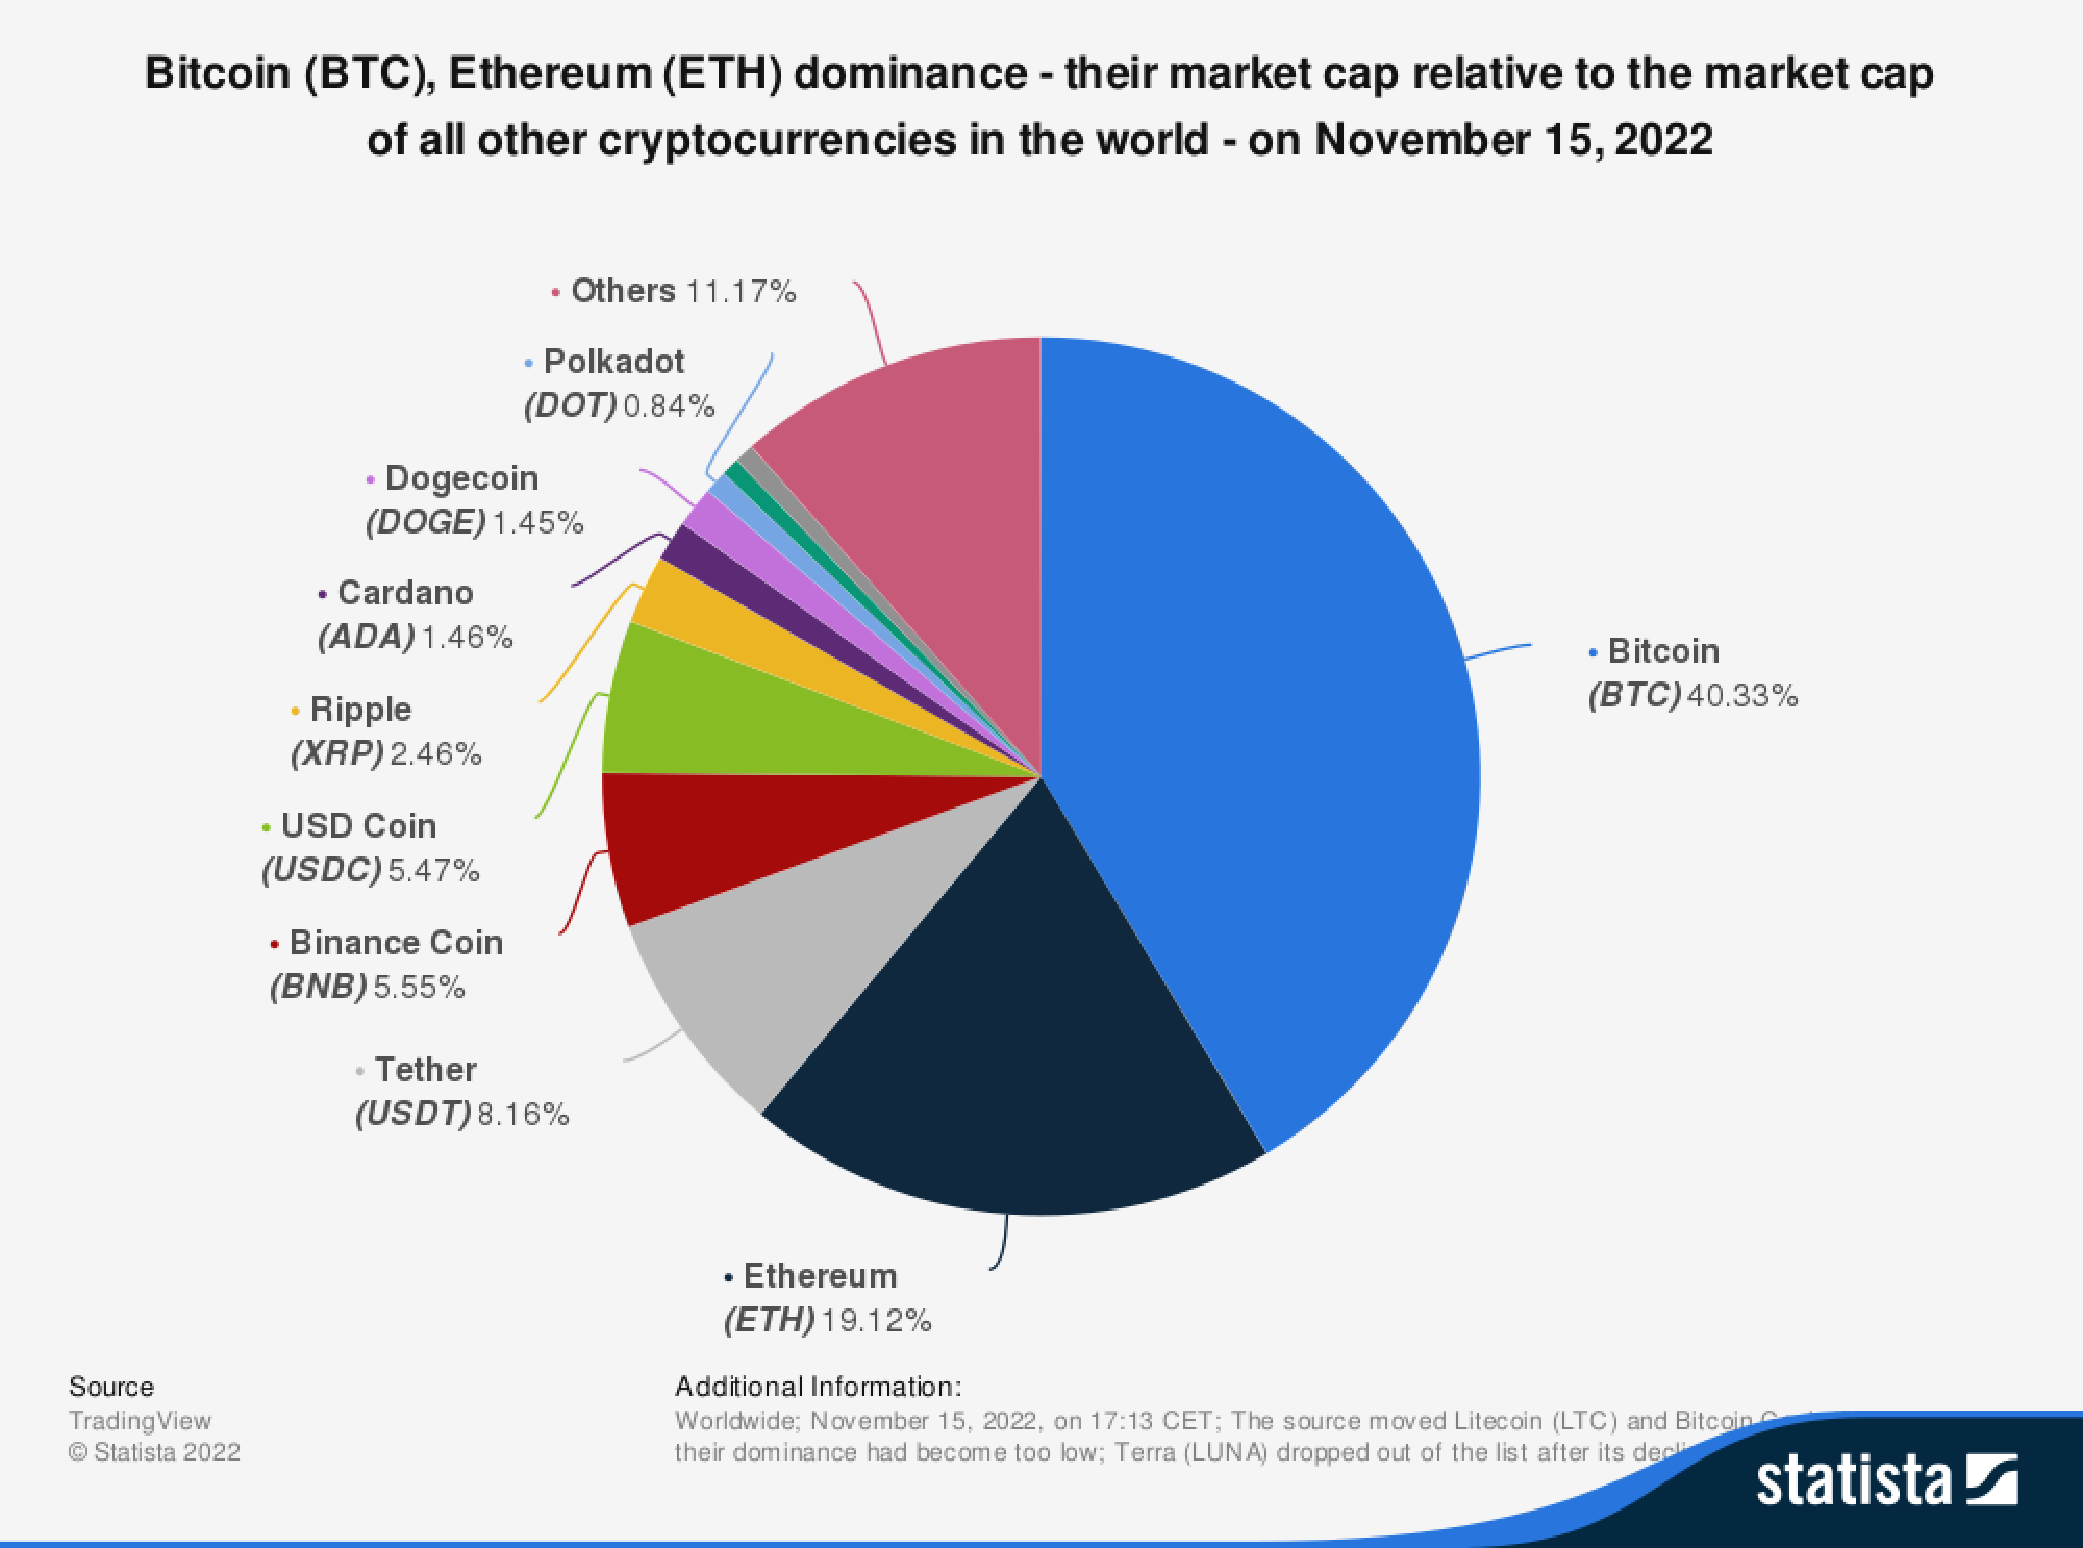
\includegraphics[scale=0.33]{Images/market_dominance.pdf}
\caption{Bitcoin (BTC), Ethereum (ETH) dominance - their market cap relative to the market cap of all other cryptocurrencies in the world - on November 15, 2022 - Statista \cite{tradingview2022}}
\label{F_market_cap}
\end{figure*}

\section{Energy consumption}

Cryptocurrencies based on proof of work, such as BTC, are known for their high electricity consumption. Elements of comparison 
are provided in this section to quantify the actual energy consumption. From the first figure (Figure \ref{F_btc_visa_energy}),
it appears that Bitcoin is consuming more electricity for one transaction, than the Visa network \emph{for 400.000 transactions}. The second figure (Figure 
\ref{F_countries_btc_energy}) highlights the energy consumption of BTC compared to entire countries. Notably, BTC consumes more electricity yearly, that Czechia 
alone.
\begin{figure*}[ht]
    \centering
     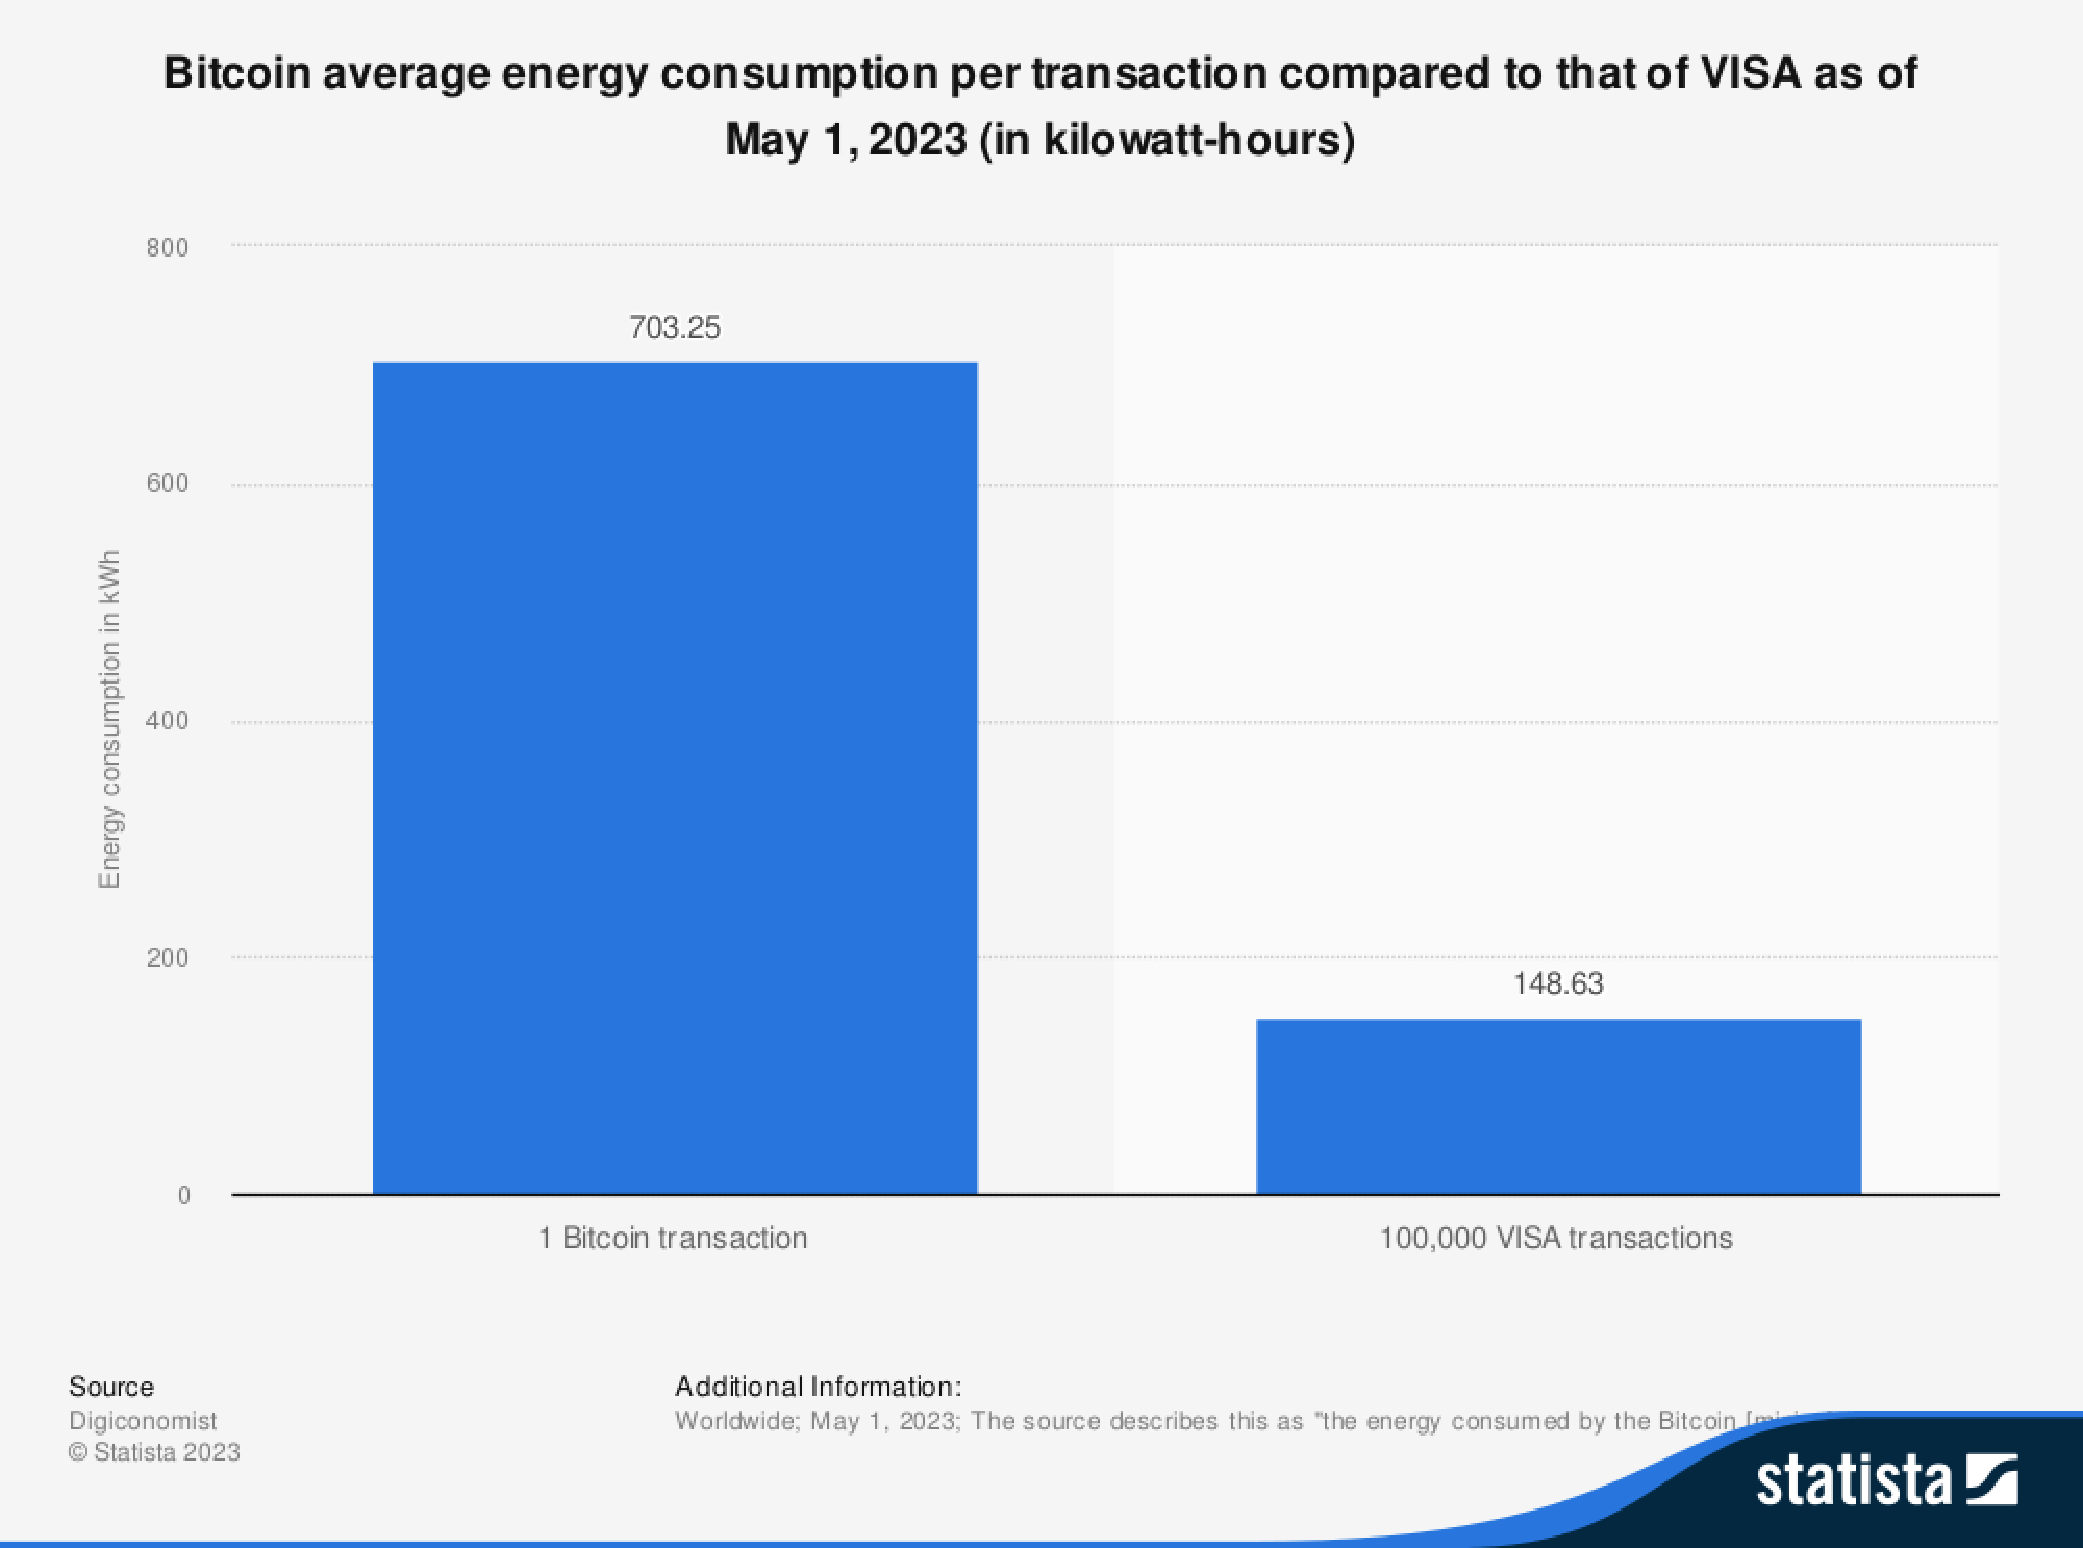
\includegraphics[scale=0.33]{Images/btc_vs_visa_energy.pdf}
    \caption{Bitcoin average energy consumption per transaction compared to that of VISA as of May 1, 2023 in kilowatt-hours - Statista \cite{Digiconomist2023}}
    \label{F_btc_visa_energy}
    \end{figure*}

    \begin{figure*}
        \centering
         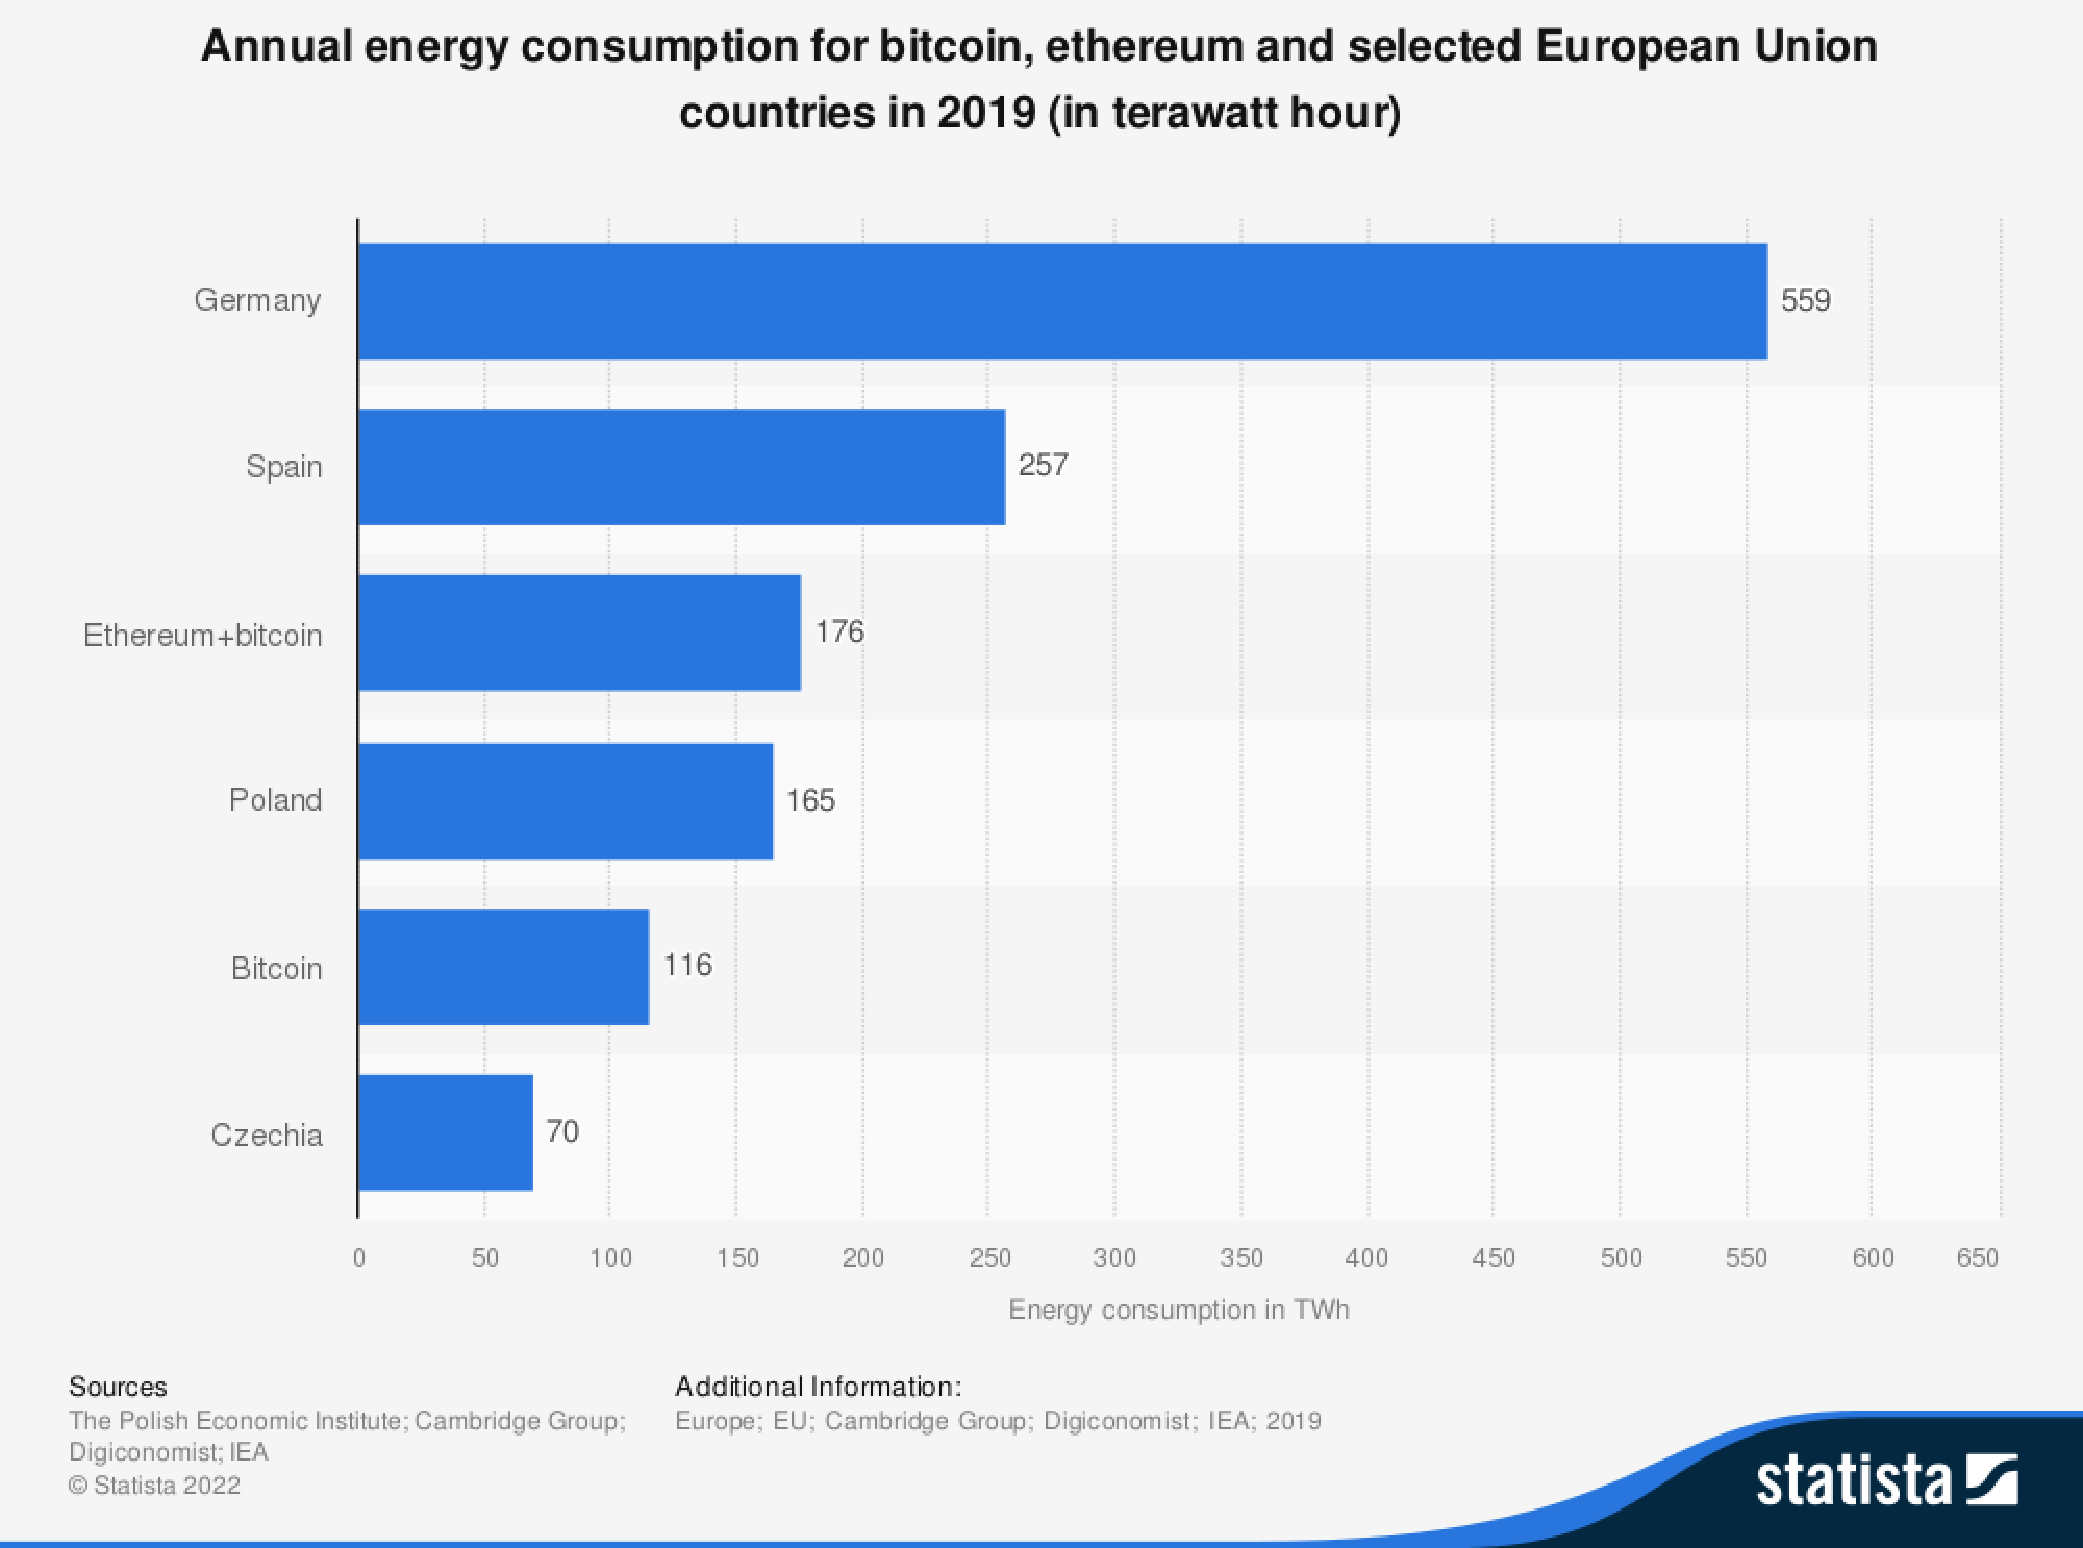
\includegraphics[scale=0.33]{Images/countries_BTC_ETH_energy.pdf}
        \caption{Annual energy consumption for bitcoin, ethereum and selected European Union countries in 2019 in terawatt hour \cite{PEI2021}}
        \label{F_countries_btc_energy}
        \end{figure*}

\section{Storage}

The Bitcoin blockchain has grown significantly since its inception to 475 GB as of June 8, 2023, and it continues to grow as new transactions are added to the network. Figure \ref{F_storage_btc} shows the evolution of Bitcoin's ledger size from 2009 to June, 2023. This continuous growth poses challenges for storage and synchronization for network participants. Running a full node, which stores a complete copy of the Bitcoin blockchain, requires substantial storage space. In addition to the blockchain data itself, a full node also needs to store additional data, such as transaction indexes and the UTXO set. As of now, a full node typically requires several terabytes of storage space.

\textbf{Pruning}. Bitcoin introduced a feature called pruning to address the storage requirements of running a full node. Pruning allows nodes to discard older blockchain data while still maintaining the ability to verify new transactions. This reduces storage requirements for nodes that do not need to maintain a complete history of all transactions.


\begin{figure*}[ht]
    \centering
     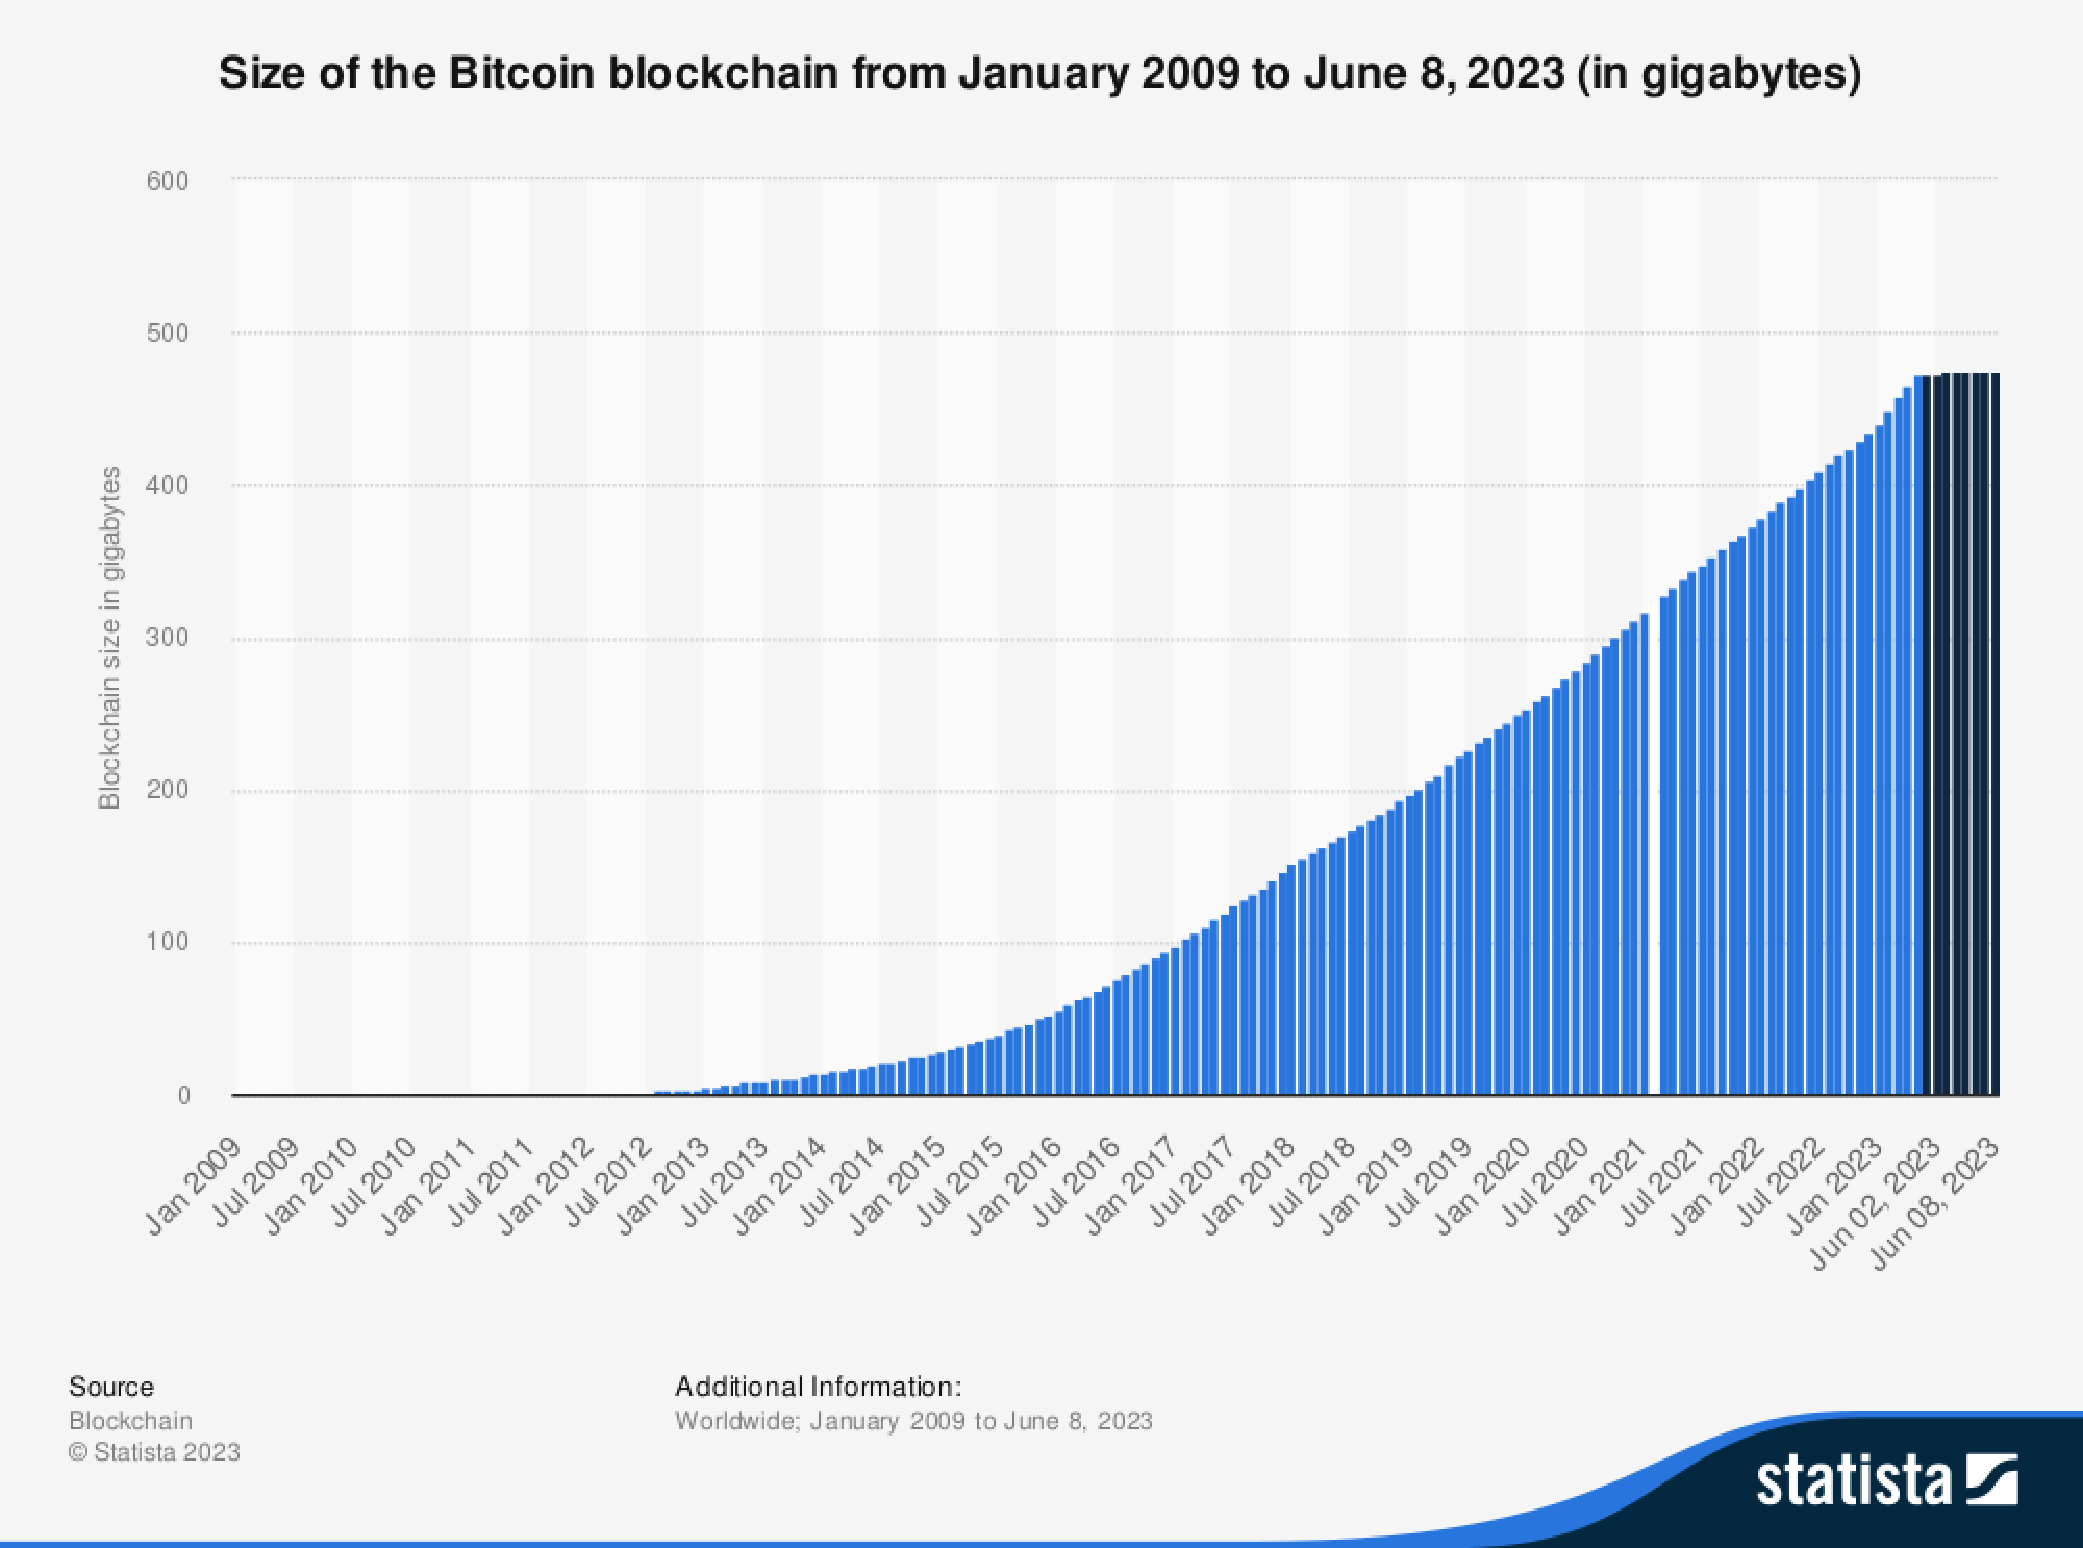
\includegraphics[scale=0.33]{Images/storage_btc.pdf}
    \caption{Size of the Bitcoin blockchain from January 2009 to June 8, 2023(in gigabytes) \cite{StatistaBTC2023}}
    \label{F_storage_btc}
    \end{figure*}

\chapter{Usage control}
\label{A_usage_control} 


The provided XACML policy (cf. Listing \ref{listing:XACML_policy}) checks if a data buyer whose address is 
\textbf{atoi1qztx22lp5n\-69f4etlr6600qcdswrj8terzkga65msddc3sh4sdx02rxjqsq}
paid the right amount of cryptocurrency (1000000) to the data provider \textbf{atoi1qpty45svr0r5s9nxatzas\-zkde8syt4etrsmea50pmc3l2swyskc0q8wlpjs}

\lstinputlisting[breaklines=true, language=XACML, caption=XACML policy, label=listing:XACML_policy]{code/policy.xml}

The XACML request (Listing \ref{listing:XACML_request})
\lstinputlisting[breaklines=true, language=XACML, caption=XACML request, label=listing:XACML_request]{code/request.xml}

%-------------------------------------------------------------------------------
\setstretch{1}
%%%%%%%%%%%%%%%%%%%%%%%%%%%%%%%%%%%%%%%%%%%%%%%%%%%%%%%%%%%%%%%%%%%%%%%%%%%%%%%%%%%%%%%%%%%%%%%%%%%%%%%%%%%%%%%%%%%%%%%%%%%%%%%%%%%%%%%%%%%%%%%%%%%%%%%%%%%%%%%%%%%%%%%
%%%%%%%%%%%%%%%%%%%%%%%%%%%%%%%%%%%%%%%%%%%%%%%%%%%%%%%%%%%%%%%%%%%%%%%%%%%%%%%%%%%%%%%%%%%%%%%%%%%%%%%%%%%%%%%%%%%%%%%%%%%%%%%%%%%%%%%%%%%%%%%%%%%%%%%%%%%%%%%%%%%%%%%
%%% Modèle pour la 4ème de couverture des thèses préparées à l'Institut Polytechnique de Paris, basé sur le modèle produit par Nikolas STOTT / Template for back cover of thesis made at Institut Polytechnique de Paris, based on the template made by Nikolas STOTT
%%% Mis à jour par Aurélien ARNOUX (École polytechnique)/ Updated by Aurélien ARNOUX (École polytechnique)
%%% Les instructions concernant chaque donnée à remplir sont données en bloc de commentaire / Rules to fill this file are given in comment blocks
%%% ATTENTION Ces informations doivent tenir sur une seule page une fois compilées / WARNING These informations must contain in no more than one page once compiled
%%%%%%%%%%%%%%%%%%%%%%%%%%%%%%%%%%%%%%%%%%%%%%%%%%%%%%%%%%%%%%%%%%%%%%%%%%%%%%%%%%%%%%%%%%%%%%%%%%%%%%%%%%%%%%%%%%%%%%%%%%%%%%%%%%%%%%%%%%%%%%%%%%%%%%%%%%%%%%%%%%%%%%%
%%% Version du 28 avril 2020 : utilisation de .png au lieu de .jpg pour les logos
%%%%%%%%%%%%%%%%%%%%%%%%%%%%%%%%%%%%%%%%%%%%%%%%%%%%%%%%%%%%%%%%%%%%%%%%%%%%%%%%%%%%%%%%%%%%%%%%%%%%%%%%%%%%%%%%%%%%%%%%%%%%%%%%%%%%%%%%%%%%%%%%%%%%%%%%%%%%%%%%%%%%%%%

% \documentclass[a4paper]{article}
% \usepackage[utf8]{inputenc}
% \usepackage{helvet}
% \renewcommand{\familydefault}{\sfdefault}
% \usepackage{geometry}
% \geometry{
% left=16mm,
% top=30mm,
% right=16mm,
% bottom=30mm
% }
% \usepackage{xcolor}
% \usepackage[absolute,overlay]{textpos}
% \usepackage{graphicx}
% \usepackage{lipsum}
% \usepackage{array}
% \usepackage{caption}
% \usepackage{multicol}
% \setlength{\columnseprule}{0pt}
% \setlength\columnsep{10pt}

% \usepackage[french]{babel}

\label{form2}
%%%%%%%%%%%%%%%%%%%%%%%%%%%%%%%%%%%%%%%%%%%%%%%%%%%%%%%%%%%%%%%%%%%%%%%%%%%%%%%%%%%%%%%%%%%%%%%%%%%%%%%%%%%%%%%%%%%%%%%%%%%%%%%%%%%%%%%%%%%%%%%%%%%%%%%%%%%%%%%%%%%%%%%
%%%%%%%%%%%%%%%%%%%%%%%%%%%%%%%%%%%%%%%%%%%%%%%%%%%%%%%%%%%%%%%%%%%%%%%%%%%%%%%%%%%%%%%%%%%%%%%%%%%%%%%%%%%%%%%%%%%%%%%%%%%%%%%%%%%%%%%%%%%%%%%%%%%%%%%%%%%%%%%%%%%%%%%
%%% Formulaire / Form
%%% Remplacer les paramètres des \newcommand par les informations demandées / Replace \newcommand parameters by asked informations
%%%%%%%%%%%%%%%%%%%%%%%%%%%%%%%%%%%%%%%%%%%%%%%%%%%%%%%%%%%%%%%%%%%%%%%%%%%%%%%%%%%%%%%%%%%%%%%%%%%%%%%%%%%%%%%%%%%%%%%%%%%%%%%%%%%%%%%%%%%%%%%%%%%%%%%%%%%%%%%%%%%%%%%
%%%%%%%%%%%%%%%%%%%%%%%%%%%%%%%%%%%%%%%%%%%%%%%%%%%%%%%%%%%%%%%%%%%%%%%%%%%%%%%%%%%%%%%%%%%%%%%%%%%%%%%%%%%%%%%%%%%%%%%%%%%%%%%%%%%%%%%%%%%%%%%%%%%%%%%%%%%%%%%%%%%%%%%


\newcommand{\logoEd}{ed}																		%% Logo de l'école doctorale. Indiquer le sigle (EDIPP, EDMH) / Doctoral school logo. Indicate the acronym : EDMH, EDIPP
\textblockcolor{white}
\newcommand{\PhDTitleFR}{Pour un internet des objets sécurisé et respectueux de la vie privée basé sur le contrôle d'usage et les registres distribués}													%% Titre de la thèse en français / Thesis title in french
\newcommand{\keywordsFR}{Internet des Objets, Systèmes distribués, Vie privée, Contrôle d'usage, RGPD}														%% Mots clés en français, séprarés par des , / Keywords in french, separated by ,
\newcommand{\abstractFR}{\lipsum[1-3]}															%% Résumé en français / abstract in french

\newcommand{\PhDTitleEN}{For a Private and Secure Internet of Things with Usage Control and Distributed Ledger Technology
}													%% Titre de la thèse en anglais / Thesis title in english
\newcommand{\keywordsEN}{Internet of Things, Distributed Systems, Privacy, Usage Control, GDPR}														%% Mots clés en anglais, séprarés par des , / Keywords in english, separated by ,
%\newcommand{\abstractEN}{\lipsum[1-3]}															%% Résumé en anglais / abstract in english

% \label{layout}
%%%%%%%%%%%%%%%%%%%%%%%%%%%%%%%%%%%%%%%%%%%%%%%%%%%%%%%%%%%%%%%%%%%%%%%%%%%%%%%%%%%%%%%%%%%%%%%%%%%%%%%%%%%%%%%%%%%%%%%%%%%%%%%%%%%%%%%%%%%%%%%%%%%%%%%%%%%%%%%%%%%%%%%
%%%%%%%%%%%%%%%%%%%%%%%%%%%%%%%%%%%%%%%%%%%%%%%%%%%%%%%%%%%%%%%%%%%%%%%%%%%%%%%%%%%%%%%%%%%%%%%%%%%%%%%%%%%%%%%%%%%%%%%%%%%%%%%%%%%%%%%%%%%%%%%%%%%%%%%%%%%%%%%%%%%%%%%
%%% Mise en page / Page layout      
%%% NE RIEN MODIFIER / DO NOT MODIFY
%%%%%%%%%%%%%%%%%%%%%%%%%%%%%%%%%%%%%%%%%%%%%%%%%%%%%%%%%%%%%%%%%%%%%%%%%%%%%%%%%%%%%%%%%%%%%%%%%%%%%%%%%%%%%%%%%%%%%%%%%%%%%%%%%%%%%%%%%%%%%%%%%%%%%%%%%%%%%%%%%%%%%%%
%%%%%%%%%%%%%%%%%%%%%%%%%%%%%%%%%%%%%%%%%%%%%%%%%%%%%%%%%%%%%%%%%%%%%%%%%%%%%%%%%%%%%%%%%%%%%%%%%%%%%%%%%%%%%%%%%%%%%%%%%%%%%%%%%%%%%%%%%%%%%%%%%%%%%%%%%%%%%%%%%%%%%%%

% \begin{document}
\pagestyle{empty}

%%% Logo de l'école doctorale. Le nom du fichier correspond au sigle de l'ED / Doctoral school logo. Filename correspond to doctoral school acronym
%%% Les noms valides sont / Valid names are : EDMH, (EDIPP)
\begin{textblock*}{61mm}(16mm,3mm)
	\noindent
\includegraphics[height=24mm]{media/ed/EDIPP-en.png}
\end{textblock*}



%%%Titre de la thèse en français / Thesis title in french
\begin{center}
\fcolorbox{black}{white}{\parbox{0.99\textwidth}{
{\bf Titre:} \PhDTitleFR 
\medskip

%%%Mots clés en français, séprarés par des ; / Keywords in french, separated by ;
{\bf Mots clés:} \keywordsFR 
\vspace{-2mm}

%%% Résumé en français / abstract in french
\begin{multicols}{2}
{\bf Résumé:} 
Les objets connectés représentent l'une des principales cibles de la cybercriminalité. Les raisons en sont multiples : d'abord, pour des raisons commerciales, les fabricants peuvent vendre des produits vulnérables qui posent des problèmes de sécurité. Deuxièmement, de nombreux appareils IoT sont soumis à des contraintes de performance et ne disposent pas de la puissance nécessaire pour exécuter des logiciels de sécurité. Enfin, l'hétérogénéité des applications, du matériel et des logiciels élargit la surface d'attaque.
Pour parer à ces menaces, l'IoT a besoin de technologies de sécurité et de préservation de la vie privée sur mesure.

 En ce qui concerne la protection de la vie privée, \emph{le contrôle d'usage} donne aux utilisateurs la possibilité de spécifier comment leurs données peuvent être utilisées et par qui. Le contrôle d'usage étend le contrôle d'accès classique en introduisant des \emph{obligations}, c'est-à-dire des actions à effectuer pour obtenir l'accès, et des \emph{conditions} qui sont liées à l'état du système, comme la charge du réseau ou le temps.
Cette thèse vise à apporter des réponses aux défis de l'internet des objets en termes de performance, de sécurité et de respect de la vie privée. Pour cela, les registres distribués (DLT) constituent une solution prometteuse aux contraintes de l'internet des objets, en particulier pour les micro-transactions, notamment par leur caractère décentralisé. Cela se traduit par trois contributions:
1. un ensemble de technologies pour des transactions sans frais préservant la vie privée, conçu pour passer à l'échelle;
2. une méthode d'intégration du contrôle d'usage et des registres distribués pour permettre une protection efficace des données des utilisateurs;
3. un modèle étendu pour le contrôle d'usage dans les systèmes distribués, afin d'y ajouter le contrôle de flux décentralisé et les aspects liés à l'internet des objets.
Une preuve de concept de l'intégration (2) a été mise en place pour démontrer la faisabilité et effectuer des tests de performance. Il s'appuie sur IOTA, un registre distribué qui utilise un graphe orienté acyclique pour son graphe de transactions au lieu d'une \emph{blockchain}. Les résultats des tests de performance sur un réseau privé montrent une diminution d'environ 90\% du temps nécessaire pour effectuer des transactions et pour évaluer des politiques de contrôle d'usage, dans le cas où ce dernier est intégré au réseau.
\end{multicols}
}}
\end{center}

\vspace*{0mm}

%%%Titre de la thèse en anglais / Thesis title in english
\begin{center}
\fcolorbox{black}{white}{\parbox{0.99\textwidth}{
{\bf Title: } \PhDTitleEN 

\medskip

%%%Mots clés en anglais, séprarés par des ; / Keywords in english, separated by ;
{\bf Keywords:}  \keywordsEN %%3 à 6 mots clés%%
\vspace{-2mm}
\begin{multicols}{2}
	
%%% Résumé en anglais / abstract in english
{\bf Abstract:} 

IoT devices represent one of the major targets for malicious activities. The grounds for this are manifold: first, to reduce the cost of security, manufacturers may sell vulnerable products, leaving users with security concerns. Second, many IoT devices have performance constraints and lack the processing power to execute security software. Third, the heterogeneity of applications, hardware, and software widens the attack surface.
As a result, IoT networks are subject to a variety of cyber threats. To counter such a variety of attacks, the IoT calls for security and privacy-preserving technologies.
%Solutions
 For privacy concerns, \emph{usage control} grants the users the power to specify how their data can be used and by whom. Usage control extends classic access control by introducing \emph{obligations}, i.e., actions to be performed to be granted access, and \emph{conditions} that are related to the system state, such as the network load or the time.
%Main contributions

This thesis aims at providing answers to the challenges in the Internet of Things in terms of performance, security and privacy. To this end, \emph{distributed ledger technologies} (DLTs) are a promising solution to Internet of Things constraints, in particular for micro-transactions, due to the decentralization they provide. This leads to three related contributions:
1. a framework for zero-fee privacy-preserving transactions in the Internet of Things designed to be scalable;
2. an integration methodology of usage control and distributed ledgers to enable efficient protection of users' data;
3. an extended model for data usage control in distributed systems, to incorporate decentralized information flow control and IoT aspects.
A proof of concept of the integration (2) has been designed to demonstrate feasibility and conduct performance tests. It is based on IOTA, a distributed ledger using a directed acyclic graph for its transaction graph instead of a blockchain. The results of the tests on a private network
show an approximate 90\% decrease in the time needed to push transactions
and make access decisions in the integrated setting.
\end{multicols}
}}
\end{center}


\begin{textblock*}{161mm}(10mm,270mm)
\color{black}
\textblockcolor{white}
{\bf\noindent Institut Polytechnique de Paris	         }

\noindent
\noindent 91120 Palaiseau, France 
\end{textblock*}

\begin{textblock*}{20mm}(175mm,265mm)
\textblockcolor{white}

\includegraphics[width=20mm]{media/IPPARIS-petit}
\end{textblock*}

% \end{document}




\end{document} 
